\documentclass[twoside]{book}

% Packages required by doxygen
\usepackage{fixltx2e}
\usepackage{calc}
\usepackage{doxygen}
\usepackage[export]{adjustbox} % also loads graphicx
\usepackage{graphicx}
\usepackage[utf8]{inputenc}
\usepackage{makeidx}
\usepackage{multicol}
\usepackage{multirow}
\PassOptionsToPackage{warn}{textcomp}
\usepackage{textcomp}
\usepackage[nointegrals]{wasysym}
\usepackage[table]{xcolor}

% Font selection
\usepackage[T1]{fontenc}
\usepackage[scaled=.90]{helvet}
\usepackage{courier}
\usepackage{amssymb}
\usepackage{sectsty}
\renewcommand{\familydefault}{\sfdefault}
\allsectionsfont{%
  \fontseries{bc}\selectfont%
  \color{darkgray}%
}
\renewcommand{\DoxyLabelFont}{%
  \fontseries{bc}\selectfont%
  \color{darkgray}%
}
\newcommand{\+}{\discretionary{\mbox{\scriptsize$\hookleftarrow$}}{}{}}

% Page & text layout
\usepackage{geometry}
\geometry{%
  a4paper,%
  top=2.5cm,%
  bottom=2.5cm,%
  left=2.5cm,%
  right=2.5cm%
}
\tolerance=750
\hfuzz=15pt
\hbadness=750
\setlength{\emergencystretch}{15pt}
\setlength{\parindent}{0cm}
\setlength{\parskip}{3ex plus 2ex minus 2ex}
\makeatletter
\renewcommand{\paragraph}{%
  \@startsection{paragraph}{4}{0ex}{-1.0ex}{1.0ex}{%
    \normalfont\normalsize\bfseries\SS@parafont%
  }%
}
\renewcommand{\subparagraph}{%
  \@startsection{subparagraph}{5}{0ex}{-1.0ex}{1.0ex}{%
    \normalfont\normalsize\bfseries\SS@subparafont%
  }%
}
\makeatother

% Headers & footers
\usepackage{fancyhdr}
\pagestyle{fancyplain}
\fancyhead[LE]{\fancyplain{}{\bfseries\thepage}}
\fancyhead[CE]{\fancyplain{}{}}
\fancyhead[RE]{\fancyplain{}{\bfseries\leftmark}}
\fancyhead[LO]{\fancyplain{}{\bfseries\rightmark}}
\fancyhead[CO]{\fancyplain{}{}}
\fancyhead[RO]{\fancyplain{}{\bfseries\thepage}}
\fancyfoot[LE]{\fancyplain{}{}}
\fancyfoot[CE]{\fancyplain{}{}}
\fancyfoot[RE]{\fancyplain{}{\bfseries\scriptsize Generated by Doxygen }}
\fancyfoot[LO]{\fancyplain{}{\bfseries\scriptsize Generated by Doxygen }}
\fancyfoot[CO]{\fancyplain{}{}}
\fancyfoot[RO]{\fancyplain{}{}}
\renewcommand{\footrulewidth}{0.4pt}
\renewcommand{\chaptermark}[1]{%
  \markboth{#1}{}%
}
\renewcommand{\sectionmark}[1]{%
  \markright{\thesection\ #1}%
}

% Indices & bibliography
\usepackage{natbib}
\usepackage[titles]{tocloft}
\setcounter{tocdepth}{3}
\setcounter{secnumdepth}{5}
\makeindex

% Hyperlinks (required, but should be loaded last)
\usepackage{ifpdf}
\ifpdf
  \usepackage[pdftex,pagebackref=true]{hyperref}
\else
  \usepackage[ps2pdf,pagebackref=true]{hyperref}
\fi
\hypersetup{%
  colorlinks=true,%
  linkcolor=blue,%
  citecolor=blue,%
  unicode%
}

% Custom commands
\newcommand{\clearemptydoublepage}{%
  \newpage{\pagestyle{empty}\cleardoublepage}%
}

\usepackage{caption}
\captionsetup{labelsep=space,justification=centering,font={bf},singlelinecheck=off,skip=4pt,position=top}

%===== C O N T E N T S =====

\begin{document}

% Titlepage & ToC
\hypersetup{pageanchor=false,
             bookmarksnumbered=true,
             pdfencoding=unicode
            }
\pagenumbering{roman}
\begin{titlepage}
\vspace*{7cm}
\begin{center}%
{\Large Snakerio }\\
\vspace*{1cm}
{\large Generated by Doxygen 1.8.11}\\
\end{center}
\end{titlepage}
\clearemptydoublepage
\tableofcontents
\clearemptydoublepage
\pagenumbering{arabic}
\hypersetup{pageanchor=true}

%--- Begin generated contents ---
\chapter{Module Index}
\section{Modules}
Here is a list of all modules\+:\begin{DoxyCompactList}
\item \contentsline{section}{Bitmap}{\pageref{group__Bitmap}}{}
\item \contentsline{section}{graphics}{\pageref{group__graphics}}{}
\item \contentsline{section}{i8254}{\pageref{group__i8254}}{}
\item \contentsline{section}{keyboard}{\pageref{group__keyboard}}{}
\item \contentsline{section}{lmlib}{\pageref{group__lmlib}}{}
\item \contentsline{section}{man\+\_\+events}{\pageref{group__man__events}}{}
\item \contentsline{section}{menu}{\pageref{group__menu}}{}
\item \contentsline{section}{mouse}{\pageref{group__mouse}}{}
\item \contentsline{section}{object}{\pageref{group__object}}{}
\item \contentsline{section}{rtc}{\pageref{group__rtc}}{}
\item \contentsline{section}{snake}{\pageref{group__snake}}{}
\item \contentsline{section}{timer}{\pageref{group__timer}}{}
\item \contentsline{section}{vbe}{\pageref{group__vbe}}{}
\item \contentsline{section}{video\+\_\+gr}{\pageref{group__video__gr}}{}
\end{DoxyCompactList}

\chapter{Class Index}
\section{Class List}
Here are the classes, structs, unions and interfaces with brief descriptions\+:\begin{DoxyCompactList}
\item\contentsline{section}{\hyperlink{struct____attribute____}{\+\_\+\+\_\+attribute\+\_\+\+\_\+} }{\pageref{struct____attribute____}}{}
\item\contentsline{section}{\hyperlink{structBitmap}{Bitmap} \\*Represents a \hyperlink{structBitmap}{Bitmap} }{\pageref{structBitmap}}{}
\item\contentsline{section}{\hyperlink{structBitmapFileHeader}{Bitmap\+File\+Header} }{\pageref{structBitmapFileHeader}}{}
\item\contentsline{section}{\hyperlink{structBitmapInfoHeader}{Bitmap\+Info\+Header} }{\pageref{structBitmapInfoHeader}}{}
\item\contentsline{section}{\hyperlink{structBitmaps__struct}{Bitmaps\+\_\+struct} }{\pageref{structBitmaps__struct}}{}
\item\contentsline{section}{\hyperlink{structdate__rtc}{date\+\_\+rtc} }{\pageref{structdate__rtc}}{}
\item\contentsline{section}{\hyperlink{structGame__object}{Game\+\_\+object} }{\pageref{structGame__object}}{}
\item\contentsline{section}{\hyperlink{structmmap__t}{mmap\+\_\+t} }{\pageref{structmmap__t}}{}
\item\contentsline{section}{\hyperlink{structSegment}{Segment} }{\pageref{structSegment}}{}
\item\contentsline{section}{\hyperlink{structSnake}{Snake} }{\pageref{structSnake}}{}
\end{DoxyCompactList}

\chapter{File Index}
\section{File List}
Here is a list of all files with brief descriptions\+:\begin{DoxyCompactList}
\item\contentsline{section}{\hyperlink{assem__scan_8d}{assem\+\_\+scan.\+d} }{\pageref{assem__scan_8d}}{}
\item\contentsline{section}{\hyperlink{Bitmap_8c}{Bitmap.\+c} }{\pageref{Bitmap_8c}}{}
\item\contentsline{section}{\hyperlink{Bitmap_8d}{Bitmap.\+d} }{\pageref{Bitmap_8d}}{}
\item\contentsline{section}{\hyperlink{Bitmap_8h}{Bitmap.\+h} }{\pageref{Bitmap_8h}}{}
\item\contentsline{section}{\hyperlink{constants_8h}{constants.\+h} }{\pageref{constants_8h}}{}
\item\contentsline{section}{\hyperlink{date_8c}{date.\+c} }{\pageref{date_8c}}{}
\item\contentsline{section}{\hyperlink{date_8d}{date.\+d} }{\pageref{date_8d}}{}
\item\contentsline{section}{\hyperlink{date_8h}{date.\+h} }{\pageref{date_8h}}{}
\item\contentsline{section}{\hyperlink{graphics_8c}{graphics.\+c} }{\pageref{graphics_8c}}{}
\item\contentsline{section}{\hyperlink{graphics_8d}{graphics.\+d} }{\pageref{graphics_8d}}{}
\item\contentsline{section}{\hyperlink{graphics_8h}{graphics.\+h} }{\pageref{graphics_8h}}{}
\item\contentsline{section}{\hyperlink{i8042_8h}{i8042.\+h} }{\pageref{i8042_8h}}{}
\item\contentsline{section}{\hyperlink{i8254_8h}{i8254.\+h} }{\pageref{i8254_8h}}{}
\item\contentsline{section}{\hyperlink{keyboard_8c}{keyboard.\+c} }{\pageref{keyboard_8c}}{}
\item\contentsline{section}{\hyperlink{keyboard_8d}{keyboard.\+d} }{\pageref{keyboard_8d}}{}
\item\contentsline{section}{\hyperlink{keyboard_8h}{keyboard.\+h} }{\pageref{keyboard_8h}}{}
\item\contentsline{section}{\hyperlink{lmlib_8h}{lmlib.\+h} }{\pageref{lmlib_8h}}{}
\item\contentsline{section}{\hyperlink{main_8c}{main.\+c} }{\pageref{main_8c}}{}
\item\contentsline{section}{\hyperlink{main_8d}{main.\+d} }{\pageref{main_8d}}{}
\item\contentsline{section}{\hyperlink{man__events_8c}{man\+\_\+events.\+c} }{\pageref{man__events_8c}}{}
\item\contentsline{section}{\hyperlink{man__events_8d}{man\+\_\+events.\+d} }{\pageref{man__events_8d}}{}
\item\contentsline{section}{\hyperlink{man__events_8h}{man\+\_\+events.\+h} }{\pageref{man__events_8h}}{}
\item\contentsline{section}{\hyperlink{menu_8c}{menu.\+c} }{\pageref{menu_8c}}{}
\item\contentsline{section}{\hyperlink{menu_8d}{menu.\+d} }{\pageref{menu_8d}}{}
\item\contentsline{section}{\hyperlink{menu_8h}{menu.\+h} }{\pageref{menu_8h}}{}
\item\contentsline{section}{\hyperlink{mouse_8c}{mouse.\+c} }{\pageref{mouse_8c}}{}
\item\contentsline{section}{\hyperlink{mouse_8d}{mouse.\+d} }{\pageref{mouse_8d}}{}
\item\contentsline{section}{\hyperlink{mouse_8h}{mouse.\+h} }{\pageref{mouse_8h}}{}
\item\contentsline{section}{\hyperlink{objects_8c}{objects.\+c} }{\pageref{objects_8c}}{}
\item\contentsline{section}{\hyperlink{objects_8d}{objects.\+d} }{\pageref{objects_8d}}{}
\item\contentsline{section}{\hyperlink{objects_8h}{objects.\+h} }{\pageref{objects_8h}}{}
\item\contentsline{section}{\hyperlink{rtc_8c}{rtc.\+c} }{\pageref{rtc_8c}}{}
\item\contentsline{section}{\hyperlink{rtc_8d}{rtc.\+d} }{\pageref{rtc_8d}}{}
\item\contentsline{section}{\hyperlink{rtc_8h}{rtc.\+h} }{\pageref{rtc_8h}}{}
\item\contentsline{section}{\hyperlink{snake_8c}{snake.\+c} }{\pageref{snake_8c}}{}
\item\contentsline{section}{\hyperlink{snake_8d}{snake.\+d} }{\pageref{snake_8d}}{}
\item\contentsline{section}{\hyperlink{snake_8h}{snake.\+h} }{\pageref{snake_8h}}{}
\item\contentsline{section}{\hyperlink{timer_8c}{timer.\+c} }{\pageref{timer_8c}}{}
\item\contentsline{section}{\hyperlink{timer_8d}{timer.\+d} }{\pageref{timer_8d}}{}
\item\contentsline{section}{\hyperlink{timer_8h}{timer.\+h} }{\pageref{timer_8h}}{}
\item\contentsline{section}{\hyperlink{vbe_8c}{vbe.\+c} }{\pageref{vbe_8c}}{}
\item\contentsline{section}{\hyperlink{vbe_8d}{vbe.\+d} }{\pageref{vbe_8d}}{}
\item\contentsline{section}{\hyperlink{vbe_8h}{vbe.\+h} }{\pageref{vbe_8h}}{}
\item\contentsline{section}{\hyperlink{video__gr_8c}{video\+\_\+gr.\+c} }{\pageref{video__gr_8c}}{}
\item\contentsline{section}{\hyperlink{video__gr_8d}{video\+\_\+gr.\+d} }{\pageref{video__gr_8d}}{}
\item\contentsline{section}{\hyperlink{video__gr_8h}{video\+\_\+gr.\+h} }{\pageref{video__gr_8h}}{}
\end{DoxyCompactList}

\chapter{Module Documentation}
\hypertarget{group__Bitmap}{}\section{Bitmap}
\label{group__Bitmap}\index{Bitmap@{Bitmap}}
\subsection*{Classes}
\begin{DoxyCompactItemize}
\item 
struct \hyperlink{structBitmapFileHeader}{Bitmap\+File\+Header}
\item 
struct \hyperlink{structBitmapInfoHeader}{Bitmap\+Info\+Header}
\item 
struct \hyperlink{structBitmap}{Bitmap}
\begin{DoxyCompactList}\small\item\em Represents a \hyperlink{structBitmap}{Bitmap}. \end{DoxyCompactList}\end{DoxyCompactItemize}
\subsection*{Enumerations}
\begin{DoxyCompactItemize}
\item 
enum \hyperlink{group__Bitmap_gacdfaca60ec19c0265bac2692d7982726}{Alignment} \{ \hyperlink{group__Bitmap_ggacdfaca60ec19c0265bac2692d7982726a6ec599857e15466988726932dd592305}{A\+L\+I\+G\+N\+\_\+\+L\+E\+FT}, 
\hyperlink{group__Bitmap_ggacdfaca60ec19c0265bac2692d7982726a5624165187e56db612253e608a45b1c6}{A\+L\+I\+G\+N\+\_\+\+C\+E\+N\+T\+ER}, 
\hyperlink{group__Bitmap_ggacdfaca60ec19c0265bac2692d7982726a9c81840e8cad46418b39a8b74a246354}{A\+L\+I\+G\+N\+\_\+\+R\+I\+G\+HT}
 \}
\end{DoxyCompactItemize}
\subsection*{Functions}
\begin{DoxyCompactItemize}
\item 
\hyperlink{structBitmap}{Bitmap} $\ast$ \hyperlink{group__Bitmap_ga3506880ffd407c36eb8aaddd2c1606d2}{load\+Bitmap} (const char $\ast$filename)
\begin{DoxyCompactList}\small\item\em Loads a bmp image. \end{DoxyCompactList}\item 
void \hyperlink{group__Bitmap_ga18d05a1c671f4638bc63d37874efb9d4}{draw\+Bitmap} (\hyperlink{structBitmap}{Bitmap} $\ast$bitmap, int x, int y, \hyperlink{group__Bitmap_gacdfaca60ec19c0265bac2692d7982726}{Alignment} alignment)
\begin{DoxyCompactList}\small\item\em Draws an unscaled, unrotated bitmap at the given position, and verify each pixel to know if it is a transparent pixel (color rgb(255, 0, 255) ) \end{DoxyCompactList}\item 
void \hyperlink{group__Bitmap_ga362eae5066441f6797d2289c5ccd493d}{drawbackground} (\hyperlink{structBitmap}{Bitmap} $\ast$\hyperlink{menu_8c_a9ac459dc630a69c0162412290c4cc1f6}{bmp}, int x, int y, \hyperlink{group__Bitmap_gacdfaca60ec19c0265bac2692d7982726}{Alignment} alignment)
\begin{DoxyCompactList}\small\item\em Draws an unscaled, unrotated bitmap at the given position. \end{DoxyCompactList}\item 
void \hyperlink{group__Bitmap_ga08c1d4f4fff81df260d979ea8fc1aa61}{delete\+Bitmap} (\hyperlink{structBitmap}{Bitmap} $\ast$\hyperlink{menu_8c_a9ac459dc630a69c0162412290c4cc1f6}{bmp})
\begin{DoxyCompactList}\small\item\em Destroys the given bitmap, freeing all resources used by it. \end{DoxyCompactList}\end{DoxyCompactItemize}
\subsection*{Variables}
\begin{DoxyCompactItemize}
\item 
static unsigned \hyperlink{group__Bitmap_ga43e7e5a0a8f9069e6413b2066ca52f3e}{h\+\_\+res}
\item 
static unsigned \hyperlink{group__Bitmap_ga5bda1b499253a8fbf3cab646f8760391}{v\+\_\+res}
\item 
static unsigned \hyperlink{group__Bitmap_ga89fa3fb58e975d148fcb2413e24b78a1}{bits\+\_\+per\+\_\+pixel}
\item 
static unsigned \hyperlink{group__Bitmap_ga59559f1bdfa71061d06d9ea27c0748ed}{screen\+\_\+size}
\end{DoxyCompactItemize}


\subsection{Detailed Description}
Functions for manipulating bitmaps 

\subsection{Enumeration Type Documentation}
\index{Bitmap@{Bitmap}!Alignment@{Alignment}}
\index{Alignment@{Alignment}!Bitmap@{Bitmap}}
\subsubsection[{\texorpdfstring{Alignment}{Alignment}}]{\setlength{\rightskip}{0pt plus 5cm}enum {\bf Alignment}}\hypertarget{group__Bitmap_gacdfaca60ec19c0265bac2692d7982726}{}\label{group__Bitmap_gacdfaca60ec19c0265bac2692d7982726}
\begin{Desc}
\item[Enumerator]\par
\begin{description}
\index{A\+L\+I\+G\+N\+\_\+\+L\+E\+FT@{A\+L\+I\+G\+N\+\_\+\+L\+E\+FT}!Bitmap@{Bitmap}}\index{Bitmap@{Bitmap}!A\+L\+I\+G\+N\+\_\+\+L\+E\+FT@{A\+L\+I\+G\+N\+\_\+\+L\+E\+FT}}\item[{\em 
A\+L\+I\+G\+N\+\_\+\+L\+E\+FT\hypertarget{group__Bitmap_ggacdfaca60ec19c0265bac2692d7982726a6ec599857e15466988726932dd592305}{}\label{group__Bitmap_ggacdfaca60ec19c0265bac2692d7982726a6ec599857e15466988726932dd592305}
}]\index{A\+L\+I\+G\+N\+\_\+\+C\+E\+N\+T\+ER@{A\+L\+I\+G\+N\+\_\+\+C\+E\+N\+T\+ER}!Bitmap@{Bitmap}}\index{Bitmap@{Bitmap}!A\+L\+I\+G\+N\+\_\+\+C\+E\+N\+T\+ER@{A\+L\+I\+G\+N\+\_\+\+C\+E\+N\+T\+ER}}\item[{\em 
A\+L\+I\+G\+N\+\_\+\+C\+E\+N\+T\+ER\hypertarget{group__Bitmap_ggacdfaca60ec19c0265bac2692d7982726a5624165187e56db612253e608a45b1c6}{}\label{group__Bitmap_ggacdfaca60ec19c0265bac2692d7982726a5624165187e56db612253e608a45b1c6}
}]\index{A\+L\+I\+G\+N\+\_\+\+R\+I\+G\+HT@{A\+L\+I\+G\+N\+\_\+\+R\+I\+G\+HT}!Bitmap@{Bitmap}}\index{Bitmap@{Bitmap}!A\+L\+I\+G\+N\+\_\+\+R\+I\+G\+HT@{A\+L\+I\+G\+N\+\_\+\+R\+I\+G\+HT}}\item[{\em 
A\+L\+I\+G\+N\+\_\+\+R\+I\+G\+HT\hypertarget{group__Bitmap_ggacdfaca60ec19c0265bac2692d7982726a9c81840e8cad46418b39a8b74a246354}{}\label{group__Bitmap_ggacdfaca60ec19c0265bac2692d7982726a9c81840e8cad46418b39a8b74a246354}
}]\end{description}
\end{Desc}


\subsection{Function Documentation}
\index{Bitmap@{Bitmap}!delete\+Bitmap@{delete\+Bitmap}}
\index{delete\+Bitmap@{delete\+Bitmap}!Bitmap@{Bitmap}}
\subsubsection[{\texorpdfstring{delete\+Bitmap(\+Bitmap $\ast$bmp)}{deleteBitmap(Bitmap *bmp)}}]{\setlength{\rightskip}{0pt plus 5cm}void delete\+Bitmap (
\begin{DoxyParamCaption}
\item[{{\bf Bitmap} $\ast$}]{bmp}
\end{DoxyParamCaption}
)}\hypertarget{group__Bitmap_ga08c1d4f4fff81df260d979ea8fc1aa61}{}\label{group__Bitmap_ga08c1d4f4fff81df260d979ea8fc1aa61}


Destroys the given bitmap, freeing all resources used by it. 


\begin{DoxyParams}{Parameters}
{\em bmp} & bitmap to be destroyed \\
\hline
\end{DoxyParams}
\index{Bitmap@{Bitmap}!drawbackground@{drawbackground}}
\index{drawbackground@{drawbackground}!Bitmap@{Bitmap}}
\subsubsection[{\texorpdfstring{drawbackground(\+Bitmap $\ast$bmp, int x, int y, Alignment alignment)}{drawbackground(Bitmap *bmp, int x, int y, Alignment alignment)}}]{\setlength{\rightskip}{0pt plus 5cm}void drawbackground (
\begin{DoxyParamCaption}
\item[{{\bf Bitmap} $\ast$}]{bmp, }
\item[{int}]{x, }
\item[{int}]{y, }
\item[{{\bf Alignment}}]{alignment}
\end{DoxyParamCaption}
)}\hypertarget{group__Bitmap_ga362eae5066441f6797d2289c5ccd493d}{}\label{group__Bitmap_ga362eae5066441f6797d2289c5ccd493d}


Draws an unscaled, unrotated bitmap at the given position. 


\begin{DoxyParams}{Parameters}
{\em bmp} & bitmap to be drawn \\
\hline
{\em x} & destiny x coord \\
\hline
{\em y} & destiny y coord \\
\hline
{\em alignment} & image alignment \\
\hline
\end{DoxyParams}


Here is the call graph for this function\+:
\nopagebreak
\begin{figure}[H]
\begin{center}
\leavevmode
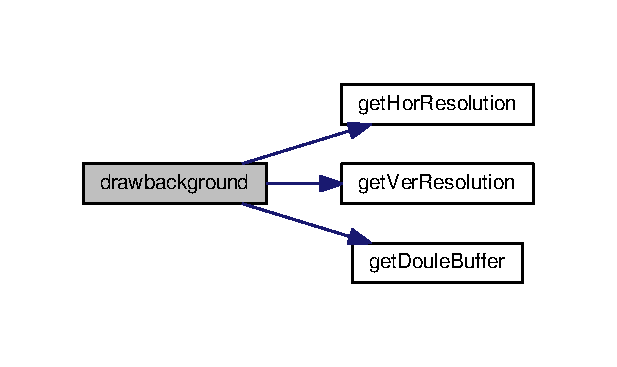
\includegraphics[width=296pt]{group__Bitmap_ga362eae5066441f6797d2289c5ccd493d_cgraph}
\end{center}
\end{figure}


\index{Bitmap@{Bitmap}!draw\+Bitmap@{draw\+Bitmap}}
\index{draw\+Bitmap@{draw\+Bitmap}!Bitmap@{Bitmap}}
\subsubsection[{\texorpdfstring{draw\+Bitmap(\+Bitmap $\ast$bitmap, int x, int y, Alignment alignment)}{drawBitmap(Bitmap *bitmap, int x, int y, Alignment alignment)}}]{\setlength{\rightskip}{0pt plus 5cm}void draw\+Bitmap (
\begin{DoxyParamCaption}
\item[{{\bf Bitmap} $\ast$}]{bitmap, }
\item[{int}]{x, }
\item[{int}]{y, }
\item[{{\bf Alignment}}]{alignment}
\end{DoxyParamCaption}
)}\hypertarget{group__Bitmap_ga18d05a1c671f4638bc63d37874efb9d4}{}\label{group__Bitmap_ga18d05a1c671f4638bc63d37874efb9d4}


Draws an unscaled, unrotated bitmap at the given position, and verify each pixel to know if it is a transparent pixel (color rgb(255, 0, 255) ) 


\begin{DoxyParams}{Parameters}
{\em bitmap} & bitmap to be drawn \\
\hline
{\em x} & destiny x coord \\
\hline
{\em y} & destiny y coord \\
\hline
{\em alignment} & image alignment \\
\hline
\end{DoxyParams}


Here is the call graph for this function\+:
\nopagebreak
\begin{figure}[H]
\begin{center}
\leavevmode
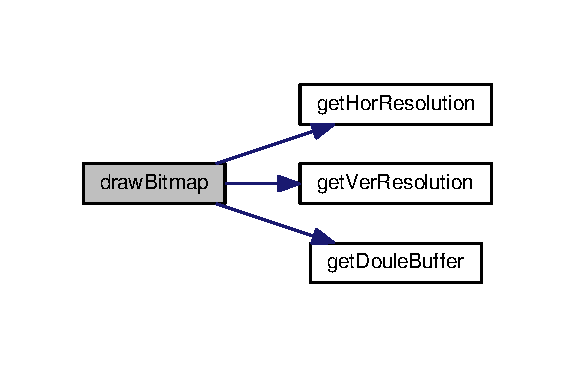
\includegraphics[width=276pt]{group__Bitmap_ga18d05a1c671f4638bc63d37874efb9d4_cgraph}
\end{center}
\end{figure}


\index{Bitmap@{Bitmap}!load\+Bitmap@{load\+Bitmap}}
\index{load\+Bitmap@{load\+Bitmap}!Bitmap@{Bitmap}}
\subsubsection[{\texorpdfstring{load\+Bitmap(const char $\ast$filename)}{loadBitmap(const char *filename)}}]{\setlength{\rightskip}{0pt plus 5cm}{\bf Bitmap}$\ast$ load\+Bitmap (
\begin{DoxyParamCaption}
\item[{const char $\ast$}]{filename}
\end{DoxyParamCaption}
)}\hypertarget{group__Bitmap_ga3506880ffd407c36eb8aaddd2c1606d2}{}\label{group__Bitmap_ga3506880ffd407c36eb8aaddd2c1606d2}


Loads a bmp image. 


\begin{DoxyParams}{Parameters}
{\em filename} & Path of the image to load \\
\hline
\end{DoxyParams}
\begin{DoxyReturn}{Returns}
Non N\+U\+LL pointer to the image buffer 
\end{DoxyReturn}


\subsection{Variable Documentation}
\index{Bitmap@{Bitmap}!bits\+\_\+per\+\_\+pixel@{bits\+\_\+per\+\_\+pixel}}
\index{bits\+\_\+per\+\_\+pixel@{bits\+\_\+per\+\_\+pixel}!Bitmap@{Bitmap}}
\subsubsection[{\texorpdfstring{bits\+\_\+per\+\_\+pixel}{bits_per_pixel}}]{\setlength{\rightskip}{0pt plus 5cm}unsigned bits\+\_\+per\+\_\+pixel\hspace{0.3cm}{\ttfamily [static]}}\hypertarget{group__Bitmap_ga89fa3fb58e975d148fcb2413e24b78a1}{}\label{group__Bitmap_ga89fa3fb58e975d148fcb2413e24b78a1}
\index{Bitmap@{Bitmap}!h\+\_\+res@{h\+\_\+res}}
\index{h\+\_\+res@{h\+\_\+res}!Bitmap@{Bitmap}}
\subsubsection[{\texorpdfstring{h\+\_\+res}{h_res}}]{\setlength{\rightskip}{0pt plus 5cm}unsigned h\+\_\+res\hspace{0.3cm}{\ttfamily [static]}}\hypertarget{group__Bitmap_ga43e7e5a0a8f9069e6413b2066ca52f3e}{}\label{group__Bitmap_ga43e7e5a0a8f9069e6413b2066ca52f3e}
\index{Bitmap@{Bitmap}!screen\+\_\+size@{screen\+\_\+size}}
\index{screen\+\_\+size@{screen\+\_\+size}!Bitmap@{Bitmap}}
\subsubsection[{\texorpdfstring{screen\+\_\+size}{screen_size}}]{\setlength{\rightskip}{0pt plus 5cm}unsigned screen\+\_\+size\hspace{0.3cm}{\ttfamily [static]}}\hypertarget{group__Bitmap_ga59559f1bdfa71061d06d9ea27c0748ed}{}\label{group__Bitmap_ga59559f1bdfa71061d06d9ea27c0748ed}
\index{Bitmap@{Bitmap}!v\+\_\+res@{v\+\_\+res}}
\index{v\+\_\+res@{v\+\_\+res}!Bitmap@{Bitmap}}
\subsubsection[{\texorpdfstring{v\+\_\+res}{v_res}}]{\setlength{\rightskip}{0pt plus 5cm}unsigned v\+\_\+res\hspace{0.3cm}{\ttfamily [static]}}\hypertarget{group__Bitmap_ga5bda1b499253a8fbf3cab646f8760391}{}\label{group__Bitmap_ga5bda1b499253a8fbf3cab646f8760391}

\hypertarget{group__graphics}{}\section{graphics}
\label{group__graphics}\index{graphics@{graphics}}
\subsection*{Classes}
\begin{DoxyCompactItemize}
\item 
struct \hyperlink{structBitmaps__struct}{Bitmaps\+\_\+struct}
\end{DoxyCompactItemize}
\subsection*{Functions}
\begin{DoxyCompactItemize}
\item 
void $\ast$ \hyperlink{group__graphics_gacef21667c79365d57a084bed994c2189}{vg\+\_\+init} (unsigned short mode)
\begin{DoxyCompactList}\small\item\em Initializes the video module in graphics mode. \end{DoxyCompactList}\item 
int \hyperlink{group__graphics_ga9805b7e746b90143a74ad077d5d68223}{vg\+\_\+exit} ()
\begin{DoxyCompactList}\small\item\em Returns to default Minix 3 text mode (0x03\+: 25 x 80, 16 colors) \end{DoxyCompactList}\item 
int \hyperlink{group__graphics_ga7d91305a8a6ade1fc8c13c1a83e011b3}{update\+\_\+matrix\+\_\+snake} (\hyperlink{structSnake}{Snake} $\ast$\hyperlink{group__man__events_gaf79c0d77b0cca9ebf96bbbed1f88aed0}{s1}, int mouse)
\begin{DoxyCompactList}\small\item\em updates the position of the snake in the screen and checks collisions \end{DoxyCompactList}\item 
void \hyperlink{group__graphics_ga6669f4e380f03339751e723309577575}{start\+\_\+mode} ()
\begin{DoxyCompactList}\small\item\em it call vg init to start the video mode in 11A and loads every bitmap used \end{DoxyCompactList}\item 
void \hyperlink{group__graphics_ga266e075db0561b07746b8dc1d6e68ccf}{clear\+\_\+matrix} ()
\begin{DoxyCompactList}\small\item\em it resets the graphics\+\_\+matrix to all N\+U\+LL pointers,so another game can be started \end{DoxyCompactList}\item 
void \hyperlink{group__graphics_gaa559040a20c89667ba7033146b4413c5}{draw\+\_\+screen} (int mode)
\begin{DoxyCompactList}\small\item\em it draws in the screen the current state of the game \end{DoxyCompactList}\item 
void \hyperlink{group__graphics_gadcd1766a79d92c6aac52fe0c7b51454c}{new\+\_\+object\+\_\+matrix} (\hyperlink{structSnake}{Snake} $\ast$\hyperlink{group__man__events_gaf79c0d77b0cca9ebf96bbbed1f88aed0}{s1}, unsigned int type)
\begin{DoxyCompactList}\small\item\em creates a new object of type type and make sure its position in the matrix doesnt interfere with the snake \end{DoxyCompactList}\item 
void \hyperlink{group__graphics_gaa03ab4855ae73e5b616cf76f54de6f76}{new\+\_\+object\+\_\+2\+\_\+snakes\+\_\+matrix} (\hyperlink{structSnake}{Snake} $\ast$\hyperlink{group__man__events_gaf79c0d77b0cca9ebf96bbbed1f88aed0}{s1}, \hyperlink{structSnake}{Snake} $\ast$\hyperlink{group__man__events_ga5b853e8b22f27ef547e5b45e4197d308}{s2}, unsigned int type)
\begin{DoxyCompactList}\small\item\em creates a new object of type type and make sure its position in the matrix doesnt interfere with the snakes \end{DoxyCompactList}\item 
void \hyperlink{group__graphics_gac6b9fb650a2fb880335948e9ef3fdf82}{remove\+\_\+snakes\+\_\+matrix} ()
\begin{DoxyCompactList}\small\item\em removes all snakes from the matrix \end{DoxyCompactList}\item 
int \hyperlink{group__graphics_gad40d6fc4b95f03cf67fff31597a2bada}{update\+\_\+matrix\+\_\+objects} (\hyperlink{structGame__object}{Game\+\_\+object} $\ast$obj, \hyperlink{structSnake}{Snake} $\ast$\hyperlink{group__man__events_gaf79c0d77b0cca9ebf96bbbed1f88aed0}{s1})
\begin{DoxyCompactList}\small\item\em places the new object created in the matrix making sure that is placed in a good spot \end{DoxyCompactList}\item 
int \hyperlink{group__graphics_ga15209d618a0ee6164a1b1c7f72ba5bdf}{update\+\_\+matrix\+\_\+objects\+\_\+2\+\_\+snakes} (\hyperlink{structGame__object}{Game\+\_\+object} $\ast$obj, \hyperlink{structSnake}{Snake} $\ast$\hyperlink{group__man__events_gaf79c0d77b0cca9ebf96bbbed1f88aed0}{s1}, \hyperlink{structSnake}{Snake} $\ast$\hyperlink{group__man__events_ga5b853e8b22f27ef547e5b45e4197d308}{s2})
\begin{DoxyCompactList}\small\item\em places the new object created in the matrix making sure that is placed in a good spot \end{DoxyCompactList}\item 
int \hyperlink{group__graphics_ga114deb65eba6094fa6251e4dbf4dc1a2}{update\+\_\+matrix\+\_\+snakemp} (\hyperlink{structSnake}{Snake} $\ast$\hyperlink{group__man__events_gaf79c0d77b0cca9ebf96bbbed1f88aed0}{s1}, \hyperlink{structSnake}{Snake} $\ast$\hyperlink{group__man__events_ga5b853e8b22f27ef547e5b45e4197d308}{s2}, int $\ast$snake1\+\_\+alive, int $\ast$snake2\+\_\+alive)
\begin{DoxyCompactList}\small\item\em it updates the matrix for the game mode with 2 snakes (similar to update matrix snake) \end{DoxyCompactList}\item 
void \hyperlink{group__graphics_ga02b1006c34287574944819caa3616660}{points\+\_\+ingame\+\_\+sp} (\hyperlink{structSnake}{Snake} $\ast$\hyperlink{group__man__events_gaf79c0d77b0cca9ebf96bbbed1f88aed0}{s1})
\begin{DoxyCompactList}\small\item\em show the points that the snake currently has during a game (game mode with only one snake) \end{DoxyCompactList}\item 
void \hyperlink{group__graphics_gaf112074b9dd511b5810d96f97e003f5e}{points\+\_\+ingame\+\_\+mp} (\hyperlink{structSnake}{Snake} $\ast$\hyperlink{group__man__events_gaf79c0d77b0cca9ebf96bbbed1f88aed0}{s1}, \hyperlink{structSnake}{Snake} $\ast$\hyperlink{group__man__events_ga5b853e8b22f27ef547e5b45e4197d308}{s2})
\begin{DoxyCompactList}\small\item\em shwo the points that both snakes has in real time during a game(game mode with 2 snakes) \end{DoxyCompactList}\item 
int \hyperlink{group__graphics_ga6e759569e268b5e7abca1e056657a608}{verify\+\_\+colision\+\_\+walls\+\_\+bgmap} (int col, int row, int mode)
\begin{DoxyCompactList}\small\item\em checks if specific place in the screen is valid(if it is not the wall of the maps used) \end{DoxyCompactList}\item 
int \hyperlink{group__graphics_ga88a7bb68362e9184035973dee2da6c83}{add\+\_\+fruit\+\_\+matrix} (int x, int y, \hyperlink{structSnake}{Snake} $\ast$\hyperlink{group__man__events_gaf79c0d77b0cca9ebf96bbbed1f88aed0}{s1})
\begin{DoxyCompactList}\small\item\em adds an object of type fruit in the position given, places only if it is valid spot (used in the mouse game mode) \end{DoxyCompactList}\item 
int \hyperlink{group__graphics_ga387f95a1f4cb68e7b372ee62064d41a5}{fruit\+\_\+count} ()
\begin{DoxyCompactList}\small\item\em counts how many fruits are in the matrix \end{DoxyCompactList}\item 
int \hyperlink{group__graphics_gaec6c3092de0056a44586f7df6de16282}{bomb\+\_\+count} ()
\begin{DoxyCompactList}\small\item\em count how many bombs are in the matrix \end{DoxyCompactList}\item 
void \hyperlink{group__graphics_gacb3ed6bc6b07cdf572291ffcea76dab8}{remove\+\_\+bomb} ()
\begin{DoxyCompactList}\small\item\em removes from the matrix the first bomb it encounters \end{DoxyCompactList}\item 
int \hyperlink{group__graphics_ga4fa3e18d37f64de83f06af9aeb725ffd}{add\+\_\+bomb\+\_\+matrix} (int x, int y, \hyperlink{structSnake}{Snake} $\ast$\hyperlink{group__man__events_gaf79c0d77b0cca9ebf96bbbed1f88aed0}{s1})
\begin{DoxyCompactList}\small\item\em adds an object of type bomb in the position given,places only if it is a valid spot(used in mouse game mode) \end{DoxyCompactList}\item 
\hyperlink{structBitmaps__struct}{Bitmaps\+\_\+struct} $\ast$ \hyperlink{group__graphics_gaec3d602834e52141c736dcc41ef0ddc9}{get\+BM} ()
\begin{DoxyCompactList}\small\item\em gets the bitmap\+\_\+struct with all bitmaps used in the project \end{DoxyCompactList}\item 
void \hyperlink{group__graphics_gaf23c56c7e38458853c7a8775fb9e09ec}{print\+\_\+number\+\_\+delay} (int \hyperlink{group__man__events_ga49dac5534222e1641ae32eba8e7baf8e}{number\+\_\+delay})
\begin{DoxyCompactList}\small\item\em Print the 3, 2, 1 numbers used when a game is starting. \end{DoxyCompactList}\end{DoxyCompactItemize}
\subsection*{Variables}
\begin{DoxyCompactItemize}
\item 
\hyperlink{structBitmap}{Bitmap} $\ast$ \hyperlink{group__graphics_ga90d36683bc99f1ee114191f6ae238990}{Bitmaps\+\_\+struct\+::maca}
\begin{DoxyCompactList}\small\item\em fruit eaten by the snake to grow \end{DoxyCompactList}\item 
\hyperlink{structBitmap}{Bitmap} $\ast$ \hyperlink{group__graphics_gaa22a993c184e8cd76dbdf4830e5d108e}{Bitmaps\+\_\+struct\+::body}
\begin{DoxyCompactList}\small\item\em body the s1 snake \end{DoxyCompactList}\item 
\hyperlink{structBitmap}{Bitmap} $\ast$ \hyperlink{group__graphics_ga8b84da2f75b89636fa34ff1cd47215f4}{Bitmaps\+\_\+struct\+::body2}
\begin{DoxyCompactList}\small\item\em body of the s2 snake \end{DoxyCompactList}\item 
\hyperlink{structBitmap}{Bitmap} $\ast$ \hyperlink{group__graphics_ga0145b28638489d1308f15646be8042eb}{Bitmaps\+\_\+struct\+::game\+\_\+over}
\item 
\hyperlink{structBitmap}{Bitmap} $\ast$ \hyperlink{group__graphics_ga2b3fa0b4fba818dec225a5cfa4ad2400}{Bitmaps\+\_\+struct\+::bg}
\begin{DoxyCompactList}\small\item\em map used in SP and \hyperlink{structSnake}{Snake} and Mouse mode \end{DoxyCompactList}\item 
\hyperlink{structBitmap}{Bitmap} $\ast$ \hyperlink{group__graphics_gaca55c5a5f1494cb6d6c872d072b501d1}{Bitmaps\+\_\+struct\+::bgmp}
\begin{DoxyCompactList}\small\item\em map used in the mode with 2 snakes \end{DoxyCompactList}\item 
\hyperlink{structBitmap}{Bitmap} $\ast$ \hyperlink{group__graphics_ga7740065d096144bd6f6f9457083584d9}{Bitmaps\+\_\+struct\+::cabeca1hd}
\begin{DoxyCompactList}\small\item\em head of the s1 snake in the horizontal and positive directions \end{DoxyCompactList}\item 
\hyperlink{structBitmap}{Bitmap} $\ast$ \hyperlink{group__graphics_ga5989c4f83267088c9fdb6d1251d2e092}{Bitmaps\+\_\+struct\+::cabeca1he}
\begin{DoxyCompactList}\small\item\em head of the s1 snake in the horizontal and negative directions \end{DoxyCompactList}\item 
\hyperlink{structBitmap}{Bitmap} $\ast$ \hyperlink{group__graphics_ga257cc4fca4ad7cceb125e4e43f62a17b}{Bitmaps\+\_\+struct\+::cabeca1vc}
\begin{DoxyCompactList}\small\item\em head of the s1 snake in the vertical and negative directions \end{DoxyCompactList}\item 
\hyperlink{structBitmap}{Bitmap} $\ast$ \hyperlink{group__graphics_ga5737d3b582663eb60cd3fd47421707b3}{Bitmaps\+\_\+struct\+::cabeca1vb}
\begin{DoxyCompactList}\small\item\em head of the s1 snake in the vertical and positive directions \end{DoxyCompactList}\item 
\hyperlink{structBitmap}{Bitmap} $\ast$ \hyperlink{group__graphics_ga74f59c6b2020b67b1e4c40b4d07b7dcb}{Bitmaps\+\_\+struct\+::cabeca2hd}
\begin{DoxyCompactList}\small\item\em head of the s2 snake in the horizontal and positive directions \end{DoxyCompactList}\item 
\hyperlink{structBitmap}{Bitmap} $\ast$ \hyperlink{group__graphics_gad921a321d31f1c5f8430770b09949bd8}{Bitmaps\+\_\+struct\+::cabeca2he}
\begin{DoxyCompactList}\small\item\em head of the s2 snake in the horizontal and negative directions \end{DoxyCompactList}\item 
\hyperlink{structBitmap}{Bitmap} $\ast$ \hyperlink{group__graphics_gabcbbaac60aafd8e9549fcef5fa6acb83}{Bitmaps\+\_\+struct\+::cabeca2vc}
\begin{DoxyCompactList}\small\item\em head of the s2 snake in the vertical and negative directions \end{DoxyCompactList}\item 
\hyperlink{structBitmap}{Bitmap} $\ast$ \hyperlink{group__graphics_ga50f31017797fe46247d3ef644f6670c9}{Bitmaps\+\_\+struct\+::cabeca2vb}
\begin{DoxyCompactList}\small\item\em head of the s2 snake in the vertical and positive directions \end{DoxyCompactList}\item 
\hyperlink{structBitmap}{Bitmap} $\ast$ \hyperlink{group__graphics_ga024eb6d4380a6df2938202e45547c241}{Bitmaps\+\_\+struct\+::main\+\_\+menu}
\begin{DoxyCompactList}\small\item\em menu that appears at the start of the game \end{DoxyCompactList}\item 
\hyperlink{structBitmap}{Bitmap} $\ast$ \hyperlink{group__graphics_ga65a5f6d63fc1498c0bace1310dac202f}{Bitmaps\+\_\+struct\+::mp\+\_\+menu}
\item 
\hyperlink{structBitmap}{Bitmap} $\ast$ \hyperlink{group__graphics_gaa9e2b675fd059f98d6fc79bff67f7918}{Bitmaps\+\_\+struct\+::cursor}
\begin{DoxyCompactList}\small\item\em menu that appears when player selects multiplayer in main\+\_\+menu \end{DoxyCompactList}\item 
\hyperlink{structBitmap}{Bitmap} $\ast$ \hyperlink{group__graphics_ga055c85bff730277d284b6e00bb7d1b62}{Bitmaps\+\_\+struct\+::numbers} \mbox{[}11\mbox{]}
\begin{DoxyCompactList}\small\item\em all the numbers from 0 to 9 in order,and the char \textquotesingle{}\+:\textquotesingle{} and \textquotesingle{}/\textquotesingle{} used in time and final scores \end{DoxyCompactList}\item 
\hyperlink{structBitmap}{Bitmap} $\ast$ \hyperlink{group__graphics_ga067f54df47f8ccad03f63d3b683f73a5}{Bitmaps\+\_\+struct\+::sp\+\_\+inst}
\begin{DoxyCompactList}\small\item\em instructions of the singleplayer mode \end{DoxyCompactList}\item 
\hyperlink{structBitmap}{Bitmap} $\ast$ \hyperlink{group__graphics_ga4096188495e68d783bf3b8ac7871b7fa}{Bitmaps\+\_\+struct\+::kbc\+\_\+inst}
\begin{DoxyCompactList}\small\item\em instructions of the snake gladiator mode \end{DoxyCompactList}\item 
\hyperlink{structBitmap}{Bitmap} $\ast$ \hyperlink{group__graphics_gaa403b7ac82d3c61224b7064f29790bd3}{Bitmaps\+\_\+struct\+::mokb\+\_\+inst}
\begin{DoxyCompactList}\small\item\em instructions of the snake and mouse game mode \end{DoxyCompactList}\item 
\hyperlink{structBitmap}{Bitmap} $\ast$ \hyperlink{group__graphics_ga3b47ad4f61b00c3e5527f2bec90890b5}{Bitmaps\+\_\+struct\+::pausesymb}
\begin{DoxyCompactList}\small\item\em pause message when the game is paused \end{DoxyCompactList}\item 
\hyperlink{structBitmap}{Bitmap} $\ast$ \hyperlink{group__graphics_ga86313247313ec7e1e264d13835d7d012}{Bitmaps\+\_\+struct\+::bomb}
\begin{DoxyCompactList}\small\item\em bomb that might kill a snake \end{DoxyCompactList}\item 
\hyperlink{structBitmap}{Bitmap} $\ast$ \hyperlink{group__graphics_gac0df1ce2b02d6d52203766b8cb13c9bf}{Bitmaps\+\_\+struct\+::explosion}
\begin{DoxyCompactList}\small\item\em explosion if snake collides with a bomb \end{DoxyCompactList}\item 
\hyperlink{structBitmap}{Bitmap} $\ast$ \hyperlink{group__graphics_gaf891e78c1cd9b89f53a3cf6032f88e71}{Bitmaps\+\_\+struct\+::press\+\_\+enter}
\begin{DoxyCompactList}\small\item\em message press enter to continue at the end of each game \end{DoxyCompactList}\item 
\hyperlink{structBitmap}{Bitmap} $\ast$ \hyperlink{group__graphics_ga279ac50f42320cb39cbc02270e40597a}{Bitmaps\+\_\+struct\+::player1}
\begin{DoxyCompactList}\small\item\em identifier of player 1 \end{DoxyCompactList}\item 
\hyperlink{structBitmap}{Bitmap} $\ast$ \hyperlink{group__graphics_gaaee24419ba914b7d473d1f5e06d84272}{Bitmaps\+\_\+struct\+::player2}
\begin{DoxyCompactList}\small\item\em identifier of player 2 \end{DoxyCompactList}\item 
\hyperlink{structBitmap}{Bitmap} $\ast$ \hyperlink{group__graphics_ga0fe961b9b328a12b933b0e3d2393e9d4}{Bitmaps\+\_\+struct\+::choose\+\_\+main}
\begin{DoxyCompactList}\small\item\em menu to choose the body and the head of the it wants to use(only in modes with one snake) \end{DoxyCompactList}\item 
\hyperlink{structBitmap}{Bitmap} $\ast$ \hyperlink{group__graphics_ga1c051bf49f7de6f60eb93649684ebfb5}{Bitmaps\+\_\+struct\+::choose\+\_\+p1}
\begin{DoxyCompactList}\small\item\em menu in 2 snakes mode, to choose the body of the snake of player1 (snake s1) \end{DoxyCompactList}\item 
\hyperlink{structBitmap}{Bitmap} $\ast$ \hyperlink{group__graphics_gabe0652c58a65bf0ccd93497ab08d9cfb}{Bitmaps\+\_\+struct\+::choose\+\_\+p2}
\begin{DoxyCompactList}\small\item\em menu in 2 snakes mode, to choose the body of the snake of player2 (snake s2) \end{DoxyCompactList}\item 
\hyperlink{structBitmap}{Bitmap} $\ast$ \hyperlink{group__graphics_ga0d2f0b6ce3ed9e3fbdca9fb0e2197c8f}{Bitmaps\+\_\+struct\+::counter1\+\_\+delay}
\begin{DoxyCompactList}\small\item\em number 1 in the countdown before the start of each game \end{DoxyCompactList}\item 
\hyperlink{structBitmap}{Bitmap} $\ast$ \hyperlink{group__graphics_gabbfd3197d8f58f68356e4c404c9b41a7}{Bitmaps\+\_\+struct\+::counter2\+\_\+delay}
\begin{DoxyCompactList}\small\item\em number 2 in the count down before the start of each game \end{DoxyCompactList}\item 
\hyperlink{structBitmap}{Bitmap} $\ast$ \hyperlink{group__graphics_gac1063b5ae836e49a51d16a672c9cc11f}{Bitmaps\+\_\+struct\+::counter3\+\_\+delay}
\begin{DoxyCompactList}\small\item\em number 3 in the count down before the start of each game \end{DoxyCompactList}\item 
\hyperlink{structBitmap}{Bitmap} $\ast$ \hyperlink{group__graphics_gac29eba55edb941d1896f1ea16ba40601}{Bitmaps\+\_\+struct\+::numbers\+\_\+score} \mbox{[}10\mbox{]}
\begin{DoxyCompactList}\small\item\em numbers from 0 to 9 used to show the atual points of the snake ingame \end{DoxyCompactList}\item 
\hyperlink{structBitmap}{Bitmap} $\ast$ \hyperlink{group__graphics_ga416a4e7839cf0a547fcf830f0e5e3cf3}{Bitmaps\+\_\+struct\+::numbers\+\_\+back}
\begin{DoxyCompactList}\small\item\em simple black background to put the numbers stated above, and to make a standard new wall that the snakes should\textquotesingle{}nt collide with \end{DoxyCompactList}\end{DoxyCompactItemize}


\subsection{Detailed Description}
Functions related to the graphics components of the game 

\subsection{Function Documentation}
\index{graphics@{graphics}!add\+\_\+bomb\+\_\+matrix@{add\+\_\+bomb\+\_\+matrix}}
\index{add\+\_\+bomb\+\_\+matrix@{add\+\_\+bomb\+\_\+matrix}!graphics@{graphics}}
\subsubsection[{\texorpdfstring{add\+\_\+bomb\+\_\+matrix(int x, int y, Snake $\ast$s1)}{add_bomb_matrix(int x, int y, Snake *s1)}}]{\setlength{\rightskip}{0pt plus 5cm}int add\+\_\+bomb\+\_\+matrix (
\begin{DoxyParamCaption}
\item[{int}]{x, }
\item[{int}]{y, }
\item[{{\bf Snake} $\ast$}]{s1}
\end{DoxyParamCaption}
)}\hypertarget{group__graphics_ga4fa3e18d37f64de83f06af9aeb725ffd}{}\label{group__graphics_ga4fa3e18d37f64de83f06af9aeb725ffd}


adds an object of type bomb in the position given,places only if it is a valid spot(used in mouse game mode) 


\begin{DoxyParams}{Parameters}
{\em x} & position on the x axis of the mouse \\
\hline
{\em y} & position on the y axis of the mouse \\
\hline
{\em s1} & snake to validate spot to put matrix ¶eturn 0 if the bomb has been successfuly added to the matrix, 1 otherwise \\
\hline
\end{DoxyParams}


Here is the call graph for this function\+:
\nopagebreak
\begin{figure}[H]
\begin{center}
\leavevmode
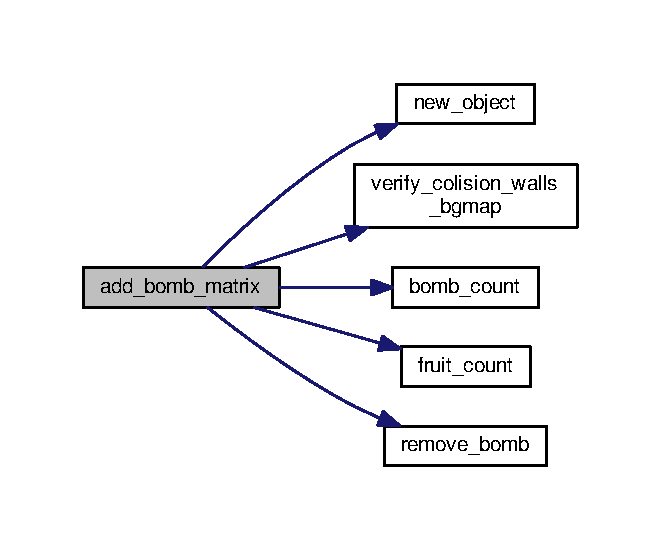
\includegraphics[width=317pt]{group__graphics_ga4fa3e18d37f64de83f06af9aeb725ffd_cgraph}
\end{center}
\end{figure}


\index{graphics@{graphics}!add\+\_\+fruit\+\_\+matrix@{add\+\_\+fruit\+\_\+matrix}}
\index{add\+\_\+fruit\+\_\+matrix@{add\+\_\+fruit\+\_\+matrix}!graphics@{graphics}}
\subsubsection[{\texorpdfstring{add\+\_\+fruit\+\_\+matrix(int x, int y, Snake $\ast$s1)}{add_fruit_matrix(int x, int y, Snake *s1)}}]{\setlength{\rightskip}{0pt plus 5cm}int add\+\_\+fruit\+\_\+matrix (
\begin{DoxyParamCaption}
\item[{int}]{x, }
\item[{int}]{y, }
\item[{{\bf Snake} $\ast$}]{s1}
\end{DoxyParamCaption}
)}\hypertarget{group__graphics_ga88a7bb68362e9184035973dee2da6c83}{}\label{group__graphics_ga88a7bb68362e9184035973dee2da6c83}


adds an object of type fruit in the position given, places only if it is valid spot (used in the mouse game mode) 


\begin{DoxyParams}{Parameters}
{\em x} & position on x axis of the mouse \\
\hline
{\em y} & position on y axis of the mouse \\
\hline
{\em s1} & snake to validate spot to put \\
\hline
\end{DoxyParams}
\begin{DoxyReturn}{Returns}
0 if the fruit has been succesfully added to the matrix, 1 otherwise 
\end{DoxyReturn}


Here is the call graph for this function\+:
\nopagebreak
\begin{figure}[H]
\begin{center}
\leavevmode
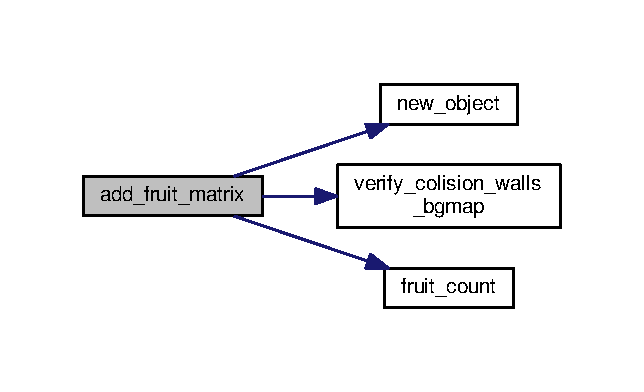
\includegraphics[width=309pt]{group__graphics_ga88a7bb68362e9184035973dee2da6c83_cgraph}
\end{center}
\end{figure}


\index{graphics@{graphics}!bomb\+\_\+count@{bomb\+\_\+count}}
\index{bomb\+\_\+count@{bomb\+\_\+count}!graphics@{graphics}}
\subsubsection[{\texorpdfstring{bomb\+\_\+count()}{bomb_count()}}]{\setlength{\rightskip}{0pt plus 5cm}int bomb\+\_\+count (
\begin{DoxyParamCaption}
{}
\end{DoxyParamCaption}
)}\hypertarget{group__graphics_gaec6c3092de0056a44586f7df6de16282}{}\label{group__graphics_gaec6c3092de0056a44586f7df6de16282}


count how many bombs are in the matrix 

\begin{DoxyReturn}{Returns}
the number of bombs in the matrix 
\end{DoxyReturn}
\index{graphics@{graphics}!clear\+\_\+matrix@{clear\+\_\+matrix}}
\index{clear\+\_\+matrix@{clear\+\_\+matrix}!graphics@{graphics}}
\subsubsection[{\texorpdfstring{clear\+\_\+matrix()}{clear_matrix()}}]{\setlength{\rightskip}{0pt plus 5cm}void clear\+\_\+matrix (
\begin{DoxyParamCaption}
{}
\end{DoxyParamCaption}
)}\hypertarget{group__graphics_ga266e075db0561b07746b8dc1d6e68ccf}{}\label{group__graphics_ga266e075db0561b07746b8dc1d6e68ccf}


it resets the graphics\+\_\+matrix to all N\+U\+LL pointers,so another game can be started 

\index{graphics@{graphics}!draw\+\_\+screen@{draw\+\_\+screen}}
\index{draw\+\_\+screen@{draw\+\_\+screen}!graphics@{graphics}}
\subsubsection[{\texorpdfstring{draw\+\_\+screen(int mode)}{draw_screen(int mode)}}]{\setlength{\rightskip}{0pt plus 5cm}void draw\+\_\+screen (
\begin{DoxyParamCaption}
\item[{int}]{mode}
\end{DoxyParamCaption}
)}\hypertarget{group__graphics_gaa559040a20c89667ba7033146b4413c5}{}\label{group__graphics_gaa559040a20c89667ba7033146b4413c5}


it draws in the screen the current state of the game 


\begin{DoxyParams}{Parameters}
{\em mode} & flag to know what map is being used \\
\hline
\end{DoxyParams}


Here is the call graph for this function\+:
\nopagebreak
\begin{figure}[H]
\begin{center}
\leavevmode
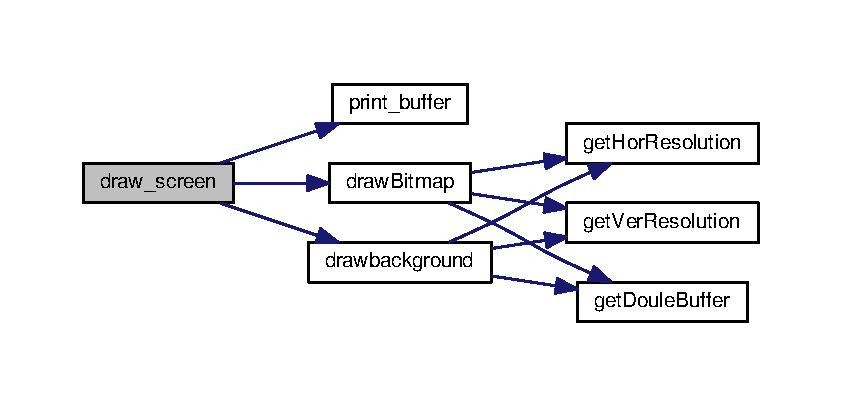
\includegraphics[width=350pt]{group__graphics_gaa559040a20c89667ba7033146b4413c5_cgraph}
\end{center}
\end{figure}


\index{graphics@{graphics}!fruit\+\_\+count@{fruit\+\_\+count}}
\index{fruit\+\_\+count@{fruit\+\_\+count}!graphics@{graphics}}
\subsubsection[{\texorpdfstring{fruit\+\_\+count()}{fruit_count()}}]{\setlength{\rightskip}{0pt plus 5cm}int fruit\+\_\+count (
\begin{DoxyParamCaption}
{}
\end{DoxyParamCaption}
)}\hypertarget{group__graphics_ga387f95a1f4cb68e7b372ee62064d41a5}{}\label{group__graphics_ga387f95a1f4cb68e7b372ee62064d41a5}


counts how many fruits are in the matrix 

\begin{DoxyReturn}{Returns}
the number of fruits in the matrix 
\end{DoxyReturn}
\index{graphics@{graphics}!get\+BM@{get\+BM}}
\index{get\+BM@{get\+BM}!graphics@{graphics}}
\subsubsection[{\texorpdfstring{get\+B\+M()}{getBM()}}]{\setlength{\rightskip}{0pt plus 5cm}{\bf Bitmaps\+\_\+struct}$\ast$ get\+BM (
\begin{DoxyParamCaption}
{}
\end{DoxyParamCaption}
)}\hypertarget{group__graphics_gaec3d602834e52141c736dcc41ef0ddc9}{}\label{group__graphics_gaec3d602834e52141c736dcc41ef0ddc9}


gets the bitmap\+\_\+struct with all bitmaps used in the project 

\begin{DoxyReturn}{Returns}
the bmp global variable 
\end{DoxyReturn}
\index{graphics@{graphics}!new\+\_\+object\+\_\+2\+\_\+snakes\+\_\+matrix@{new\+\_\+object\+\_\+2\+\_\+snakes\+\_\+matrix}}
\index{new\+\_\+object\+\_\+2\+\_\+snakes\+\_\+matrix@{new\+\_\+object\+\_\+2\+\_\+snakes\+\_\+matrix}!graphics@{graphics}}
\subsubsection[{\texorpdfstring{new\+\_\+object\+\_\+2\+\_\+snakes\+\_\+matrix(\+Snake $\ast$s1, Snake $\ast$s2, unsigned int type)}{new_object_2_snakes_matrix(Snake *s1, Snake *s2, unsigned int type)}}]{\setlength{\rightskip}{0pt plus 5cm}void new\+\_\+object\+\_\+2\+\_\+snakes\+\_\+matrix (
\begin{DoxyParamCaption}
\item[{{\bf Snake} $\ast$}]{s1, }
\item[{{\bf Snake} $\ast$}]{s2, }
\item[{unsigned int}]{type}
\end{DoxyParamCaption}
)}\hypertarget{group__graphics_gaa03ab4855ae73e5b616cf76f54de6f76}{}\label{group__graphics_gaa03ab4855ae73e5b616cf76f54de6f76}


creates a new object of type type and make sure its position in the matrix doesnt interfere with the snakes 


\begin{DoxyParams}{Parameters}
{\em s1} & snake to compare positions with \\
\hline
{\em s2} & second snake to compare positions with \\
\hline
{\em type} & what type of object it is (0 for fruit or 1 for bomb) \\
\hline
\end{DoxyParams}


Here is the call graph for this function\+:
\nopagebreak
\begin{figure}[H]
\begin{center}
\leavevmode
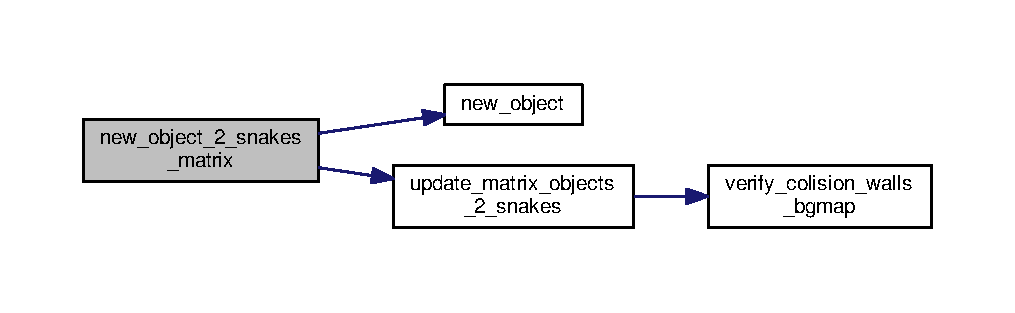
\includegraphics[width=350pt]{group__graphics_gaa03ab4855ae73e5b616cf76f54de6f76_cgraph}
\end{center}
\end{figure}


\index{graphics@{graphics}!new\+\_\+object\+\_\+matrix@{new\+\_\+object\+\_\+matrix}}
\index{new\+\_\+object\+\_\+matrix@{new\+\_\+object\+\_\+matrix}!graphics@{graphics}}
\subsubsection[{\texorpdfstring{new\+\_\+object\+\_\+matrix(\+Snake $\ast$s1, unsigned int type)}{new_object_matrix(Snake *s1, unsigned int type)}}]{\setlength{\rightskip}{0pt plus 5cm}void new\+\_\+object\+\_\+matrix (
\begin{DoxyParamCaption}
\item[{{\bf Snake} $\ast$}]{s1, }
\item[{unsigned int}]{type}
\end{DoxyParamCaption}
)}\hypertarget{group__graphics_gadcd1766a79d92c6aac52fe0c7b51454c}{}\label{group__graphics_gadcd1766a79d92c6aac52fe0c7b51454c}


creates a new object of type type and make sure its position in the matrix doesnt interfere with the snake 


\begin{DoxyParams}{Parameters}
{\em s1} & snake to compare positions wiht \\
\hline
{\em type} & what type of object it is (0 for fruit or 1 for bomb) \\
\hline
\end{DoxyParams}


Here is the call graph for this function\+:
\nopagebreak
\begin{figure}[H]
\begin{center}
\leavevmode
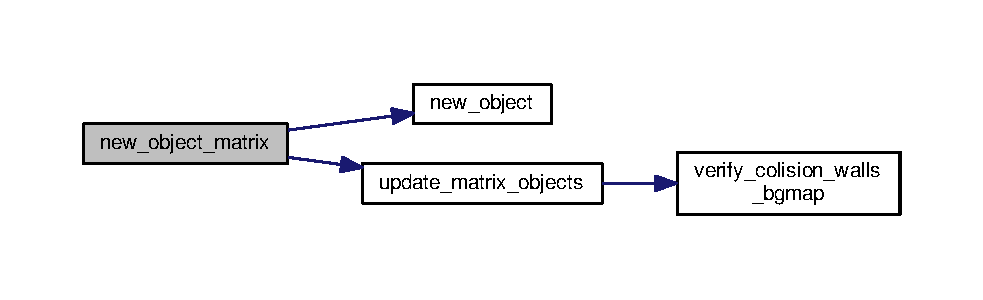
\includegraphics[width=350pt]{group__graphics_gadcd1766a79d92c6aac52fe0c7b51454c_cgraph}
\end{center}
\end{figure}


\index{graphics@{graphics}!points\+\_\+ingame\+\_\+mp@{points\+\_\+ingame\+\_\+mp}}
\index{points\+\_\+ingame\+\_\+mp@{points\+\_\+ingame\+\_\+mp}!graphics@{graphics}}
\subsubsection[{\texorpdfstring{points\+\_\+ingame\+\_\+mp(\+Snake $\ast$s1, Snake $\ast$s2)}{points_ingame_mp(Snake *s1, Snake *s2)}}]{\setlength{\rightskip}{0pt plus 5cm}void points\+\_\+ingame\+\_\+mp (
\begin{DoxyParamCaption}
\item[{{\bf Snake} $\ast$}]{s1, }
\item[{{\bf Snake} $\ast$}]{s2}
\end{DoxyParamCaption}
)}\hypertarget{group__graphics_gaf112074b9dd511b5810d96f97e003f5e}{}\label{group__graphics_gaf112074b9dd511b5810d96f97e003f5e}


shwo the points that both snakes has in real time during a game(game mode with 2 snakes) 


\begin{DoxyParams}{Parameters}
{\em s1} & snake to check points of player 1 \\
\hline
{\em s2} & snake to check points of player 2 \\
\hline
\end{DoxyParams}


Here is the call graph for this function\+:
\nopagebreak
\begin{figure}[H]
\begin{center}
\leavevmode
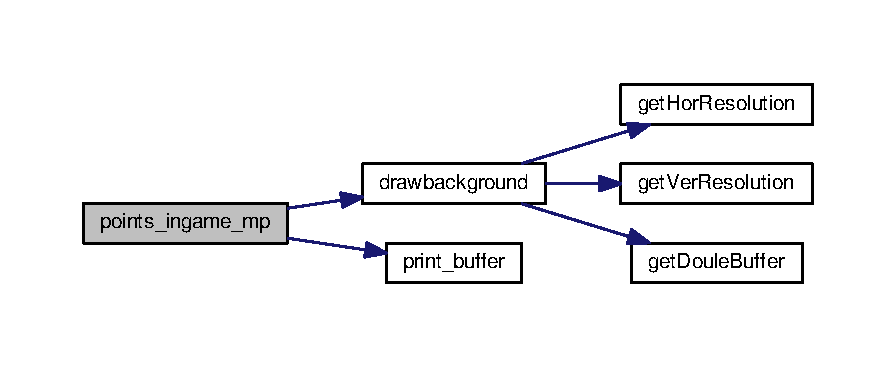
\includegraphics[width=350pt]{group__graphics_gaf112074b9dd511b5810d96f97e003f5e_cgraph}
\end{center}
\end{figure}


\index{graphics@{graphics}!points\+\_\+ingame\+\_\+sp@{points\+\_\+ingame\+\_\+sp}}
\index{points\+\_\+ingame\+\_\+sp@{points\+\_\+ingame\+\_\+sp}!graphics@{graphics}}
\subsubsection[{\texorpdfstring{points\+\_\+ingame\+\_\+sp(\+Snake $\ast$s1)}{points_ingame_sp(Snake *s1)}}]{\setlength{\rightskip}{0pt plus 5cm}void points\+\_\+ingame\+\_\+sp (
\begin{DoxyParamCaption}
\item[{{\bf Snake} $\ast$}]{s1}
\end{DoxyParamCaption}
)}\hypertarget{group__graphics_ga02b1006c34287574944819caa3616660}{}\label{group__graphics_ga02b1006c34287574944819caa3616660}


show the points that the snake currently has during a game (game mode with only one snake) 


\begin{DoxyParams}{Parameters}
{\em s1} & snake to check its points \\
\hline
\end{DoxyParams}


Here is the call graph for this function\+:
\nopagebreak
\begin{figure}[H]
\begin{center}
\leavevmode
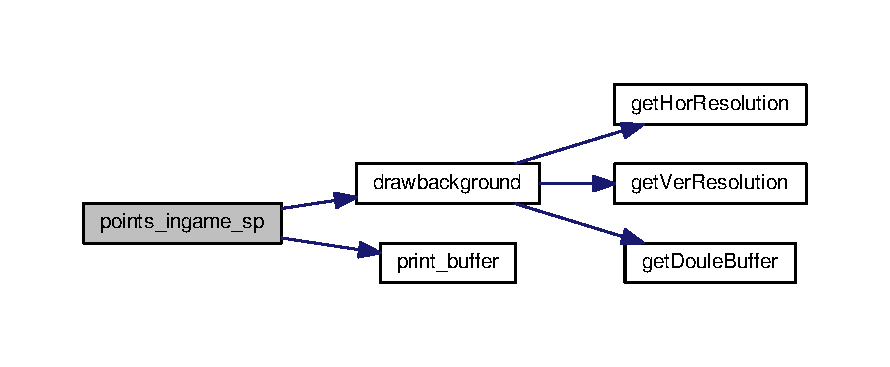
\includegraphics[width=350pt]{group__graphics_ga02b1006c34287574944819caa3616660_cgraph}
\end{center}
\end{figure}


\index{graphics@{graphics}!print\+\_\+number\+\_\+delay@{print\+\_\+number\+\_\+delay}}
\index{print\+\_\+number\+\_\+delay@{print\+\_\+number\+\_\+delay}!graphics@{graphics}}
\subsubsection[{\texorpdfstring{print\+\_\+number\+\_\+delay(int number\+\_\+delay)}{print_number_delay(int number_delay)}}]{\setlength{\rightskip}{0pt plus 5cm}void print\+\_\+number\+\_\+delay (
\begin{DoxyParamCaption}
\item[{int}]{number\+\_\+delay}
\end{DoxyParamCaption}
)}\hypertarget{group__graphics_gaf23c56c7e38458853c7a8775fb9e09ec}{}\label{group__graphics_gaf23c56c7e38458853c7a8775fb9e09ec}


Print the 3, 2, 1 numbers used when a game is starting. 


\begin{DoxyParams}{Parameters}
{\em number\+\_\+delay} & Number to print (1, 2 or 3) \\
\hline
\end{DoxyParams}


Here is the call graph for this function\+:
\nopagebreak
\begin{figure}[H]
\begin{center}
\leavevmode
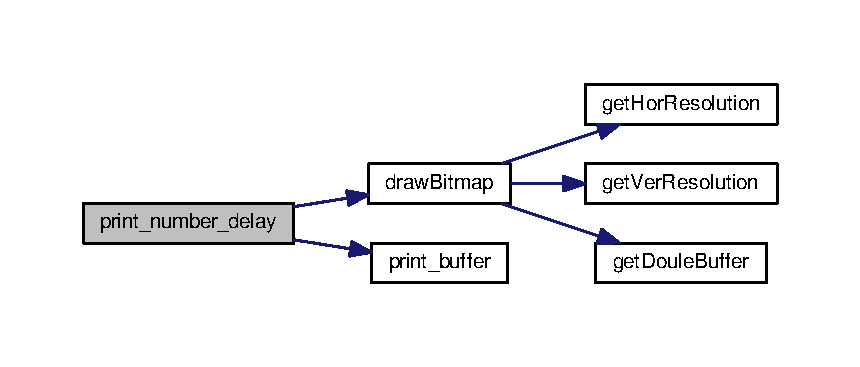
\includegraphics[width=350pt]{group__graphics_gaf23c56c7e38458853c7a8775fb9e09ec_cgraph}
\end{center}
\end{figure}


\index{graphics@{graphics}!remove\+\_\+bomb@{remove\+\_\+bomb}}
\index{remove\+\_\+bomb@{remove\+\_\+bomb}!graphics@{graphics}}
\subsubsection[{\texorpdfstring{remove\+\_\+bomb()}{remove_bomb()}}]{\setlength{\rightskip}{0pt plus 5cm}void remove\+\_\+bomb (
\begin{DoxyParamCaption}
{}
\end{DoxyParamCaption}
)}\hypertarget{group__graphics_gacb3ed6bc6b07cdf572291ffcea76dab8}{}\label{group__graphics_gacb3ed6bc6b07cdf572291ffcea76dab8}


removes from the matrix the first bomb it encounters 

\index{graphics@{graphics}!remove\+\_\+snakes\+\_\+matrix@{remove\+\_\+snakes\+\_\+matrix}}
\index{remove\+\_\+snakes\+\_\+matrix@{remove\+\_\+snakes\+\_\+matrix}!graphics@{graphics}}
\subsubsection[{\texorpdfstring{remove\+\_\+snakes\+\_\+matrix()}{remove_snakes_matrix()}}]{\setlength{\rightskip}{0pt plus 5cm}void remove\+\_\+snakes\+\_\+matrix (
\begin{DoxyParamCaption}
{}
\end{DoxyParamCaption}
)}\hypertarget{group__graphics_gac6b9fb650a2fb880335948e9ef3fdf82}{}\label{group__graphics_gac6b9fb650a2fb880335948e9ef3fdf82}


removes all snakes from the matrix 

\index{graphics@{graphics}!start\+\_\+mode@{start\+\_\+mode}}
\index{start\+\_\+mode@{start\+\_\+mode}!graphics@{graphics}}
\subsubsection[{\texorpdfstring{start\+\_\+mode()}{start_mode()}}]{\setlength{\rightskip}{0pt plus 5cm}void start\+\_\+mode (
\begin{DoxyParamCaption}
{}
\end{DoxyParamCaption}
)}\hypertarget{group__graphics_ga6669f4e380f03339751e723309577575}{}\label{group__graphics_ga6669f4e380f03339751e723309577575}


it call vg init to start the video mode in 11A and loads every bitmap used 



Here is the call graph for this function\+:
\nopagebreak
\begin{figure}[H]
\begin{center}
\leavevmode
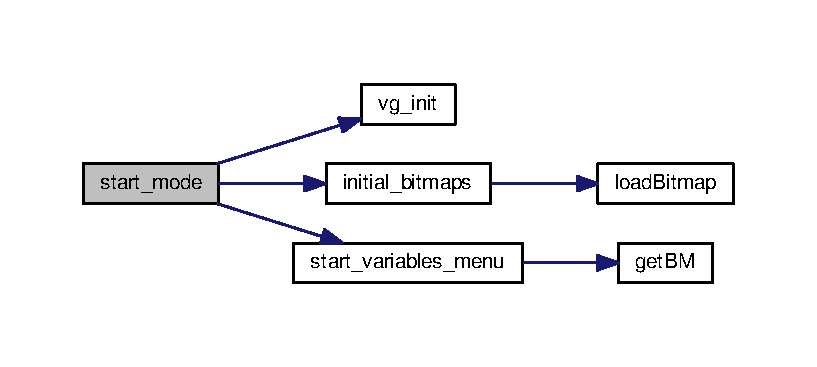
\includegraphics[width=350pt]{group__graphics_ga6669f4e380f03339751e723309577575_cgraph}
\end{center}
\end{figure}


\index{graphics@{graphics}!update\+\_\+matrix\+\_\+objects@{update\+\_\+matrix\+\_\+objects}}
\index{update\+\_\+matrix\+\_\+objects@{update\+\_\+matrix\+\_\+objects}!graphics@{graphics}}
\subsubsection[{\texorpdfstring{update\+\_\+matrix\+\_\+objects(\+Game\+\_\+object $\ast$obj, Snake $\ast$s1)}{update_matrix_objects(Game_object *obj, Snake *s1)}}]{\setlength{\rightskip}{0pt plus 5cm}int update\+\_\+matrix\+\_\+objects (
\begin{DoxyParamCaption}
\item[{{\bf Game\+\_\+object} $\ast$}]{obj, }
\item[{{\bf Snake} $\ast$}]{s1}
\end{DoxyParamCaption}
)}\hypertarget{group__graphics_gad40d6fc4b95f03cf67fff31597a2bada}{}\label{group__graphics_gad40d6fc4b95f03cf67fff31597a2bada}


places the new object created in the matrix making sure that is placed in a good spot 


\begin{DoxyParams}{Parameters}
{\em obj} & object that is being set \\
\hline
{\em s1} & snake to compare if it is placed on a good spot \\
\hline
\end{DoxyParams}
\begin{DoxyReturn}{Returns}
0 if has been successfully placed,1 otherwise 
\end{DoxyReturn}


Here is the call graph for this function\+:
\nopagebreak
\begin{figure}[H]
\begin{center}
\leavevmode
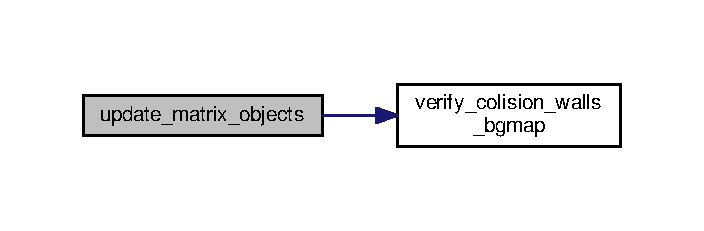
\includegraphics[width=338pt]{group__graphics_gad40d6fc4b95f03cf67fff31597a2bada_cgraph}
\end{center}
\end{figure}


\index{graphics@{graphics}!update\+\_\+matrix\+\_\+objects\+\_\+2\+\_\+snakes@{update\+\_\+matrix\+\_\+objects\+\_\+2\+\_\+snakes}}
\index{update\+\_\+matrix\+\_\+objects\+\_\+2\+\_\+snakes@{update\+\_\+matrix\+\_\+objects\+\_\+2\+\_\+snakes}!graphics@{graphics}}
\subsubsection[{\texorpdfstring{update\+\_\+matrix\+\_\+objects\+\_\+2\+\_\+snakes(\+Game\+\_\+object $\ast$obj, Snake $\ast$s1, Snake $\ast$s2)}{update_matrix_objects_2_snakes(Game_object *obj, Snake *s1, Snake *s2)}}]{\setlength{\rightskip}{0pt plus 5cm}int update\+\_\+matrix\+\_\+objects\+\_\+2\+\_\+snakes (
\begin{DoxyParamCaption}
\item[{{\bf Game\+\_\+object} $\ast$}]{obj, }
\item[{{\bf Snake} $\ast$}]{s1, }
\item[{{\bf Snake} $\ast$}]{s2}
\end{DoxyParamCaption}
)}\hypertarget{group__graphics_ga15209d618a0ee6164a1b1c7f72ba5bdf}{}\label{group__graphics_ga15209d618a0ee6164a1b1c7f72ba5bdf}


places the new object created in the matrix making sure that is placed in a good spot 


\begin{DoxyParams}{Parameters}
{\em obj} & object that is being set \\
\hline
{\em s1} & snake to compare if it is placed on a good spot \\
\hline
{\em s2} & second snake to compare if it is placed on a good spot \\
\hline
\end{DoxyParams}
\begin{DoxyReturn}{Returns}
0 if has been successfully placed,1 otherwise 
\end{DoxyReturn}


Here is the call graph for this function\+:
\nopagebreak
\begin{figure}[H]
\begin{center}
\leavevmode
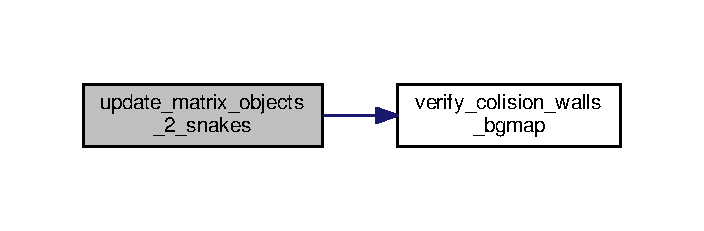
\includegraphics[width=338pt]{group__graphics_ga15209d618a0ee6164a1b1c7f72ba5bdf_cgraph}
\end{center}
\end{figure}


\index{graphics@{graphics}!update\+\_\+matrix\+\_\+snake@{update\+\_\+matrix\+\_\+snake}}
\index{update\+\_\+matrix\+\_\+snake@{update\+\_\+matrix\+\_\+snake}!graphics@{graphics}}
\subsubsection[{\texorpdfstring{update\+\_\+matrix\+\_\+snake(\+Snake $\ast$s1, int mouse)}{update_matrix_snake(Snake *s1, int mouse)}}]{\setlength{\rightskip}{0pt plus 5cm}int update\+\_\+matrix\+\_\+snake (
\begin{DoxyParamCaption}
\item[{{\bf Snake} $\ast$}]{s1, }
\item[{int}]{mouse}
\end{DoxyParamCaption}
)}\hypertarget{group__graphics_ga7d91305a8a6ade1fc8c13c1a83e011b3}{}\label{group__graphics_ga7d91305a8a6ade1fc8c13c1a83e011b3}


updates the position of the snake in the screen and checks collisions 


\begin{DoxyParams}{Parameters}
{\em s1} & snake that is going to be analised and update in the matrix \\
\hline
{\em mouse} & flag to know if when a snake collides with a fruit (eats it) to know if a new fruit should be generated automatically,or if the game mode is snake and mouse and doesnt need to do it \\
\hline
\end{DoxyParams}
\begin{DoxyReturn}{Returns}
1 if the snake as collided with something other than a fruit, so we know the snake dies,return 0 if the snake is ok 
\end{DoxyReturn}


Here is the call graph for this function\+:
\nopagebreak
\begin{figure}[H]
\begin{center}
\leavevmode
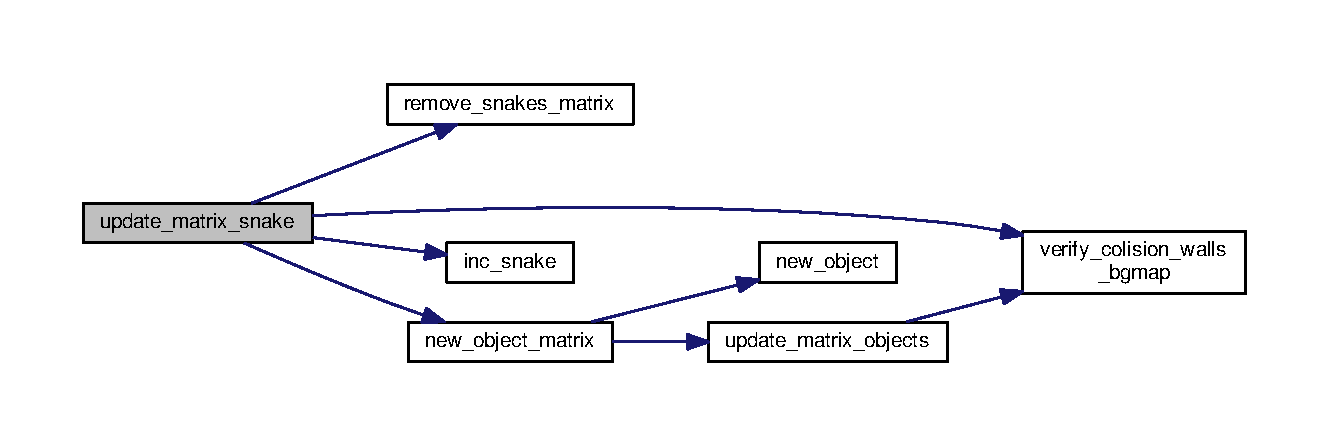
\includegraphics[width=350pt]{group__graphics_ga7d91305a8a6ade1fc8c13c1a83e011b3_cgraph}
\end{center}
\end{figure}


\index{graphics@{graphics}!update\+\_\+matrix\+\_\+snakemp@{update\+\_\+matrix\+\_\+snakemp}}
\index{update\+\_\+matrix\+\_\+snakemp@{update\+\_\+matrix\+\_\+snakemp}!graphics@{graphics}}
\subsubsection[{\texorpdfstring{update\+\_\+matrix\+\_\+snakemp(\+Snake $\ast$s1, Snake $\ast$s2, int $\ast$snake1\+\_\+alive, int $\ast$snake2\+\_\+alive)}{update_matrix_snakemp(Snake *s1, Snake *s2, int *snake1_alive, int *snake2_alive)}}]{\setlength{\rightskip}{0pt plus 5cm}int update\+\_\+matrix\+\_\+snakemp (
\begin{DoxyParamCaption}
\item[{{\bf Snake} $\ast$}]{s1, }
\item[{{\bf Snake} $\ast$}]{s2, }
\item[{int $\ast$}]{snake1\+\_\+alive, }
\item[{int $\ast$}]{snake2\+\_\+alive}
\end{DoxyParamCaption}
)}\hypertarget{group__graphics_ga114deb65eba6094fa6251e4dbf4dc1a2}{}\label{group__graphics_ga114deb65eba6094fa6251e4dbf4dc1a2}


it updates the matrix for the game mode with 2 snakes (similar to update matrix snake) 


\begin{DoxyParams}{Parameters}
{\em s1} & snake of player 1 that is being updated in the matrix \\
\hline
{\em s2} & snake of player 2 that is being updated in the matrix \\
\hline
{\em snake1\+\_\+alive} & flag to know the living state of snake1 (so the game doesnt end when one of the snakes dies) \\
\hline
{\em snake2\+\_\+alive} & flag to know the living state of snake2 \\
\hline
\end{DoxyParams}
\begin{DoxyReturn}{Returns}
1 if any of the snakes has collided with a dangerous object,otherwise returns 0 
\end{DoxyReturn}


Here is the call graph for this function\+:
\nopagebreak
\begin{figure}[H]
\begin{center}
\leavevmode
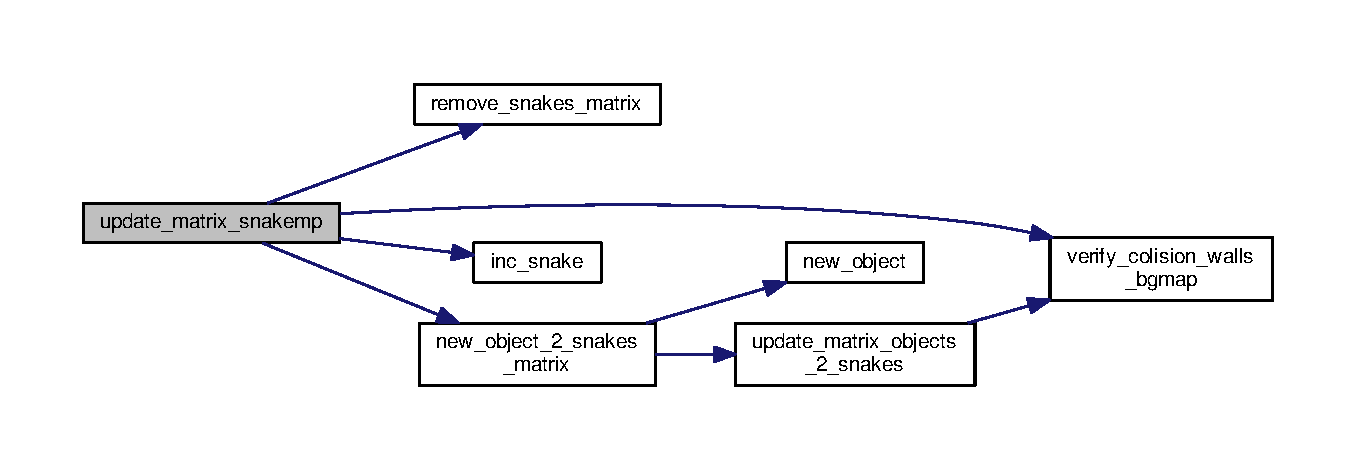
\includegraphics[width=350pt]{group__graphics_ga114deb65eba6094fa6251e4dbf4dc1a2_cgraph}
\end{center}
\end{figure}


\index{graphics@{graphics}!verify\+\_\+colision\+\_\+walls\+\_\+bgmap@{verify\+\_\+colision\+\_\+walls\+\_\+bgmap}}
\index{verify\+\_\+colision\+\_\+walls\+\_\+bgmap@{verify\+\_\+colision\+\_\+walls\+\_\+bgmap}!graphics@{graphics}}
\subsubsection[{\texorpdfstring{verify\+\_\+colision\+\_\+walls\+\_\+bgmap(int col, int row, int mode)}{verify_colision_walls_bgmap(int col, int row, int mode)}}]{\setlength{\rightskip}{0pt plus 5cm}int verify\+\_\+colision\+\_\+walls\+\_\+bgmap (
\begin{DoxyParamCaption}
\item[{int}]{col, }
\item[{int}]{row, }
\item[{int}]{mode}
\end{DoxyParamCaption}
)}\hypertarget{group__graphics_ga6e759569e268b5e7abca1e056657a608}{}\label{group__graphics_ga6e759569e268b5e7abca1e056657a608}


checks if specific place in the screen is valid(if it is not the wall of the maps used) 


\begin{DoxyParams}{Parameters}
{\em col} & column that is going to be studied \\
\hline
{\em row} & row that is being studied \\
\hline
{\em mode} & to check what map we are checking collisions, 1 for map with only one snake , 2 for the other map \\
\hline
\end{DoxyParams}
\begin{DoxyReturn}{Returns}
1 if it is an invalid place(if it is in a same position with a wall of the map), 0 otherwise 
\end{DoxyReturn}
\index{graphics@{graphics}!vg\+\_\+exit@{vg\+\_\+exit}}
\index{vg\+\_\+exit@{vg\+\_\+exit}!graphics@{graphics}}
\subsubsection[{\texorpdfstring{vg\+\_\+exit()}{vg_exit()}}]{\setlength{\rightskip}{0pt plus 5cm}int vg\+\_\+exit (
\begin{DoxyParamCaption}
{}
\end{DoxyParamCaption}
)}\hypertarget{group__graphics_ga9805b7e746b90143a74ad077d5d68223}{}\label{group__graphics_ga9805b7e746b90143a74ad077d5d68223}


Returns to default Minix 3 text mode (0x03\+: 25 x 80, 16 colors) 

\begin{DoxyReturn}{Returns}
0 upon success, non-\/zero upon failure 
\end{DoxyReturn}
\index{graphics@{graphics}!vg\+\_\+init@{vg\+\_\+init}}
\index{vg\+\_\+init@{vg\+\_\+init}!graphics@{graphics}}
\subsubsection[{\texorpdfstring{vg\+\_\+init(unsigned short mode)}{vg_init(unsigned short mode)}}]{\setlength{\rightskip}{0pt plus 5cm}void$\ast$ vg\+\_\+init (
\begin{DoxyParamCaption}
\item[{unsigned short}]{mode}
\end{DoxyParamCaption}
)}\hypertarget{group__graphics_gacef21667c79365d57a084bed994c2189}{}\label{group__graphics_gacef21667c79365d57a084bed994c2189}


Initializes the video module in graphics mode. 

Uses the V\+BE I\+NT 0x10 interface to set the desired graphics mode, maps V\+R\+AM to the process\textquotesingle{} address space and initializes global variables with the resolution of the screen, and the number of colors


\begin{DoxyParams}{Parameters}
{\em mode} & 16-\/bit V\+BE mode to set \\
\hline
\end{DoxyParams}
\begin{DoxyReturn}{Returns}
Virtual address V\+R\+AM was mapped to. N\+U\+LL, upon failure. 
\end{DoxyReturn}


\subsection{Variable Documentation}
\index{graphics@{graphics}!bg@{bg}}
\index{bg@{bg}!graphics@{graphics}}
\subsubsection[{\texorpdfstring{bg}{bg}}]{\setlength{\rightskip}{0pt plus 5cm}{\bf Bitmap}$\ast$ Bitmaps\+\_\+struct\+::bg}\hypertarget{group__graphics_ga2b3fa0b4fba818dec225a5cfa4ad2400}{}\label{group__graphics_ga2b3fa0b4fba818dec225a5cfa4ad2400}


map used in SP and \hyperlink{structSnake}{Snake} and Mouse mode 

\index{graphics@{graphics}!bgmp@{bgmp}}
\index{bgmp@{bgmp}!graphics@{graphics}}
\subsubsection[{\texorpdfstring{bgmp}{bgmp}}]{\setlength{\rightskip}{0pt plus 5cm}{\bf Bitmap}$\ast$ Bitmaps\+\_\+struct\+::bgmp}\hypertarget{group__graphics_gaca55c5a5f1494cb6d6c872d072b501d1}{}\label{group__graphics_gaca55c5a5f1494cb6d6c872d072b501d1}


map used in the mode with 2 snakes 

\index{graphics@{graphics}!body@{body}}
\index{body@{body}!graphics@{graphics}}
\subsubsection[{\texorpdfstring{body}{body}}]{\setlength{\rightskip}{0pt plus 5cm}{\bf Bitmap}$\ast$ Bitmaps\+\_\+struct\+::body}\hypertarget{group__graphics_gaa22a993c184e8cd76dbdf4830e5d108e}{}\label{group__graphics_gaa22a993c184e8cd76dbdf4830e5d108e}


body the s1 snake 

\index{graphics@{graphics}!body2@{body2}}
\index{body2@{body2}!graphics@{graphics}}
\subsubsection[{\texorpdfstring{body2}{body2}}]{\setlength{\rightskip}{0pt plus 5cm}{\bf Bitmap}$\ast$ Bitmaps\+\_\+struct\+::body2}\hypertarget{group__graphics_ga8b84da2f75b89636fa34ff1cd47215f4}{}\label{group__graphics_ga8b84da2f75b89636fa34ff1cd47215f4}


body of the s2 snake 

\index{graphics@{graphics}!bomb@{bomb}}
\index{bomb@{bomb}!graphics@{graphics}}
\subsubsection[{\texorpdfstring{bomb}{bomb}}]{\setlength{\rightskip}{0pt plus 5cm}{\bf Bitmap}$\ast$ Bitmaps\+\_\+struct\+::bomb}\hypertarget{group__graphics_ga86313247313ec7e1e264d13835d7d012}{}\label{group__graphics_ga86313247313ec7e1e264d13835d7d012}


bomb that might kill a snake 

\index{graphics@{graphics}!cabeca1hd@{cabeca1hd}}
\index{cabeca1hd@{cabeca1hd}!graphics@{graphics}}
\subsubsection[{\texorpdfstring{cabeca1hd}{cabeca1hd}}]{\setlength{\rightskip}{0pt plus 5cm}{\bf Bitmap}$\ast$ Bitmaps\+\_\+struct\+::cabeca1hd}\hypertarget{group__graphics_ga7740065d096144bd6f6f9457083584d9}{}\label{group__graphics_ga7740065d096144bd6f6f9457083584d9}


head of the s1 snake in the horizontal and positive directions 

\index{graphics@{graphics}!cabeca1he@{cabeca1he}}
\index{cabeca1he@{cabeca1he}!graphics@{graphics}}
\subsubsection[{\texorpdfstring{cabeca1he}{cabeca1he}}]{\setlength{\rightskip}{0pt plus 5cm}{\bf Bitmap}$\ast$ Bitmaps\+\_\+struct\+::cabeca1he}\hypertarget{group__graphics_ga5989c4f83267088c9fdb6d1251d2e092}{}\label{group__graphics_ga5989c4f83267088c9fdb6d1251d2e092}


head of the s1 snake in the horizontal and negative directions 

\index{graphics@{graphics}!cabeca1vb@{cabeca1vb}}
\index{cabeca1vb@{cabeca1vb}!graphics@{graphics}}
\subsubsection[{\texorpdfstring{cabeca1vb}{cabeca1vb}}]{\setlength{\rightskip}{0pt plus 5cm}{\bf Bitmap}$\ast$ Bitmaps\+\_\+struct\+::cabeca1vb}\hypertarget{group__graphics_ga5737d3b582663eb60cd3fd47421707b3}{}\label{group__graphics_ga5737d3b582663eb60cd3fd47421707b3}


head of the s1 snake in the vertical and positive directions 

\index{graphics@{graphics}!cabeca1vc@{cabeca1vc}}
\index{cabeca1vc@{cabeca1vc}!graphics@{graphics}}
\subsubsection[{\texorpdfstring{cabeca1vc}{cabeca1vc}}]{\setlength{\rightskip}{0pt plus 5cm}{\bf Bitmap}$\ast$ Bitmaps\+\_\+struct\+::cabeca1vc}\hypertarget{group__graphics_ga257cc4fca4ad7cceb125e4e43f62a17b}{}\label{group__graphics_ga257cc4fca4ad7cceb125e4e43f62a17b}


head of the s1 snake in the vertical and negative directions 

\index{graphics@{graphics}!cabeca2hd@{cabeca2hd}}
\index{cabeca2hd@{cabeca2hd}!graphics@{graphics}}
\subsubsection[{\texorpdfstring{cabeca2hd}{cabeca2hd}}]{\setlength{\rightskip}{0pt plus 5cm}{\bf Bitmap}$\ast$ Bitmaps\+\_\+struct\+::cabeca2hd}\hypertarget{group__graphics_ga74f59c6b2020b67b1e4c40b4d07b7dcb}{}\label{group__graphics_ga74f59c6b2020b67b1e4c40b4d07b7dcb}


head of the s2 snake in the horizontal and positive directions 

\index{graphics@{graphics}!cabeca2he@{cabeca2he}}
\index{cabeca2he@{cabeca2he}!graphics@{graphics}}
\subsubsection[{\texorpdfstring{cabeca2he}{cabeca2he}}]{\setlength{\rightskip}{0pt plus 5cm}{\bf Bitmap}$\ast$ Bitmaps\+\_\+struct\+::cabeca2he}\hypertarget{group__graphics_gad921a321d31f1c5f8430770b09949bd8}{}\label{group__graphics_gad921a321d31f1c5f8430770b09949bd8}


head of the s2 snake in the horizontal and negative directions 

\index{graphics@{graphics}!cabeca2vb@{cabeca2vb}}
\index{cabeca2vb@{cabeca2vb}!graphics@{graphics}}
\subsubsection[{\texorpdfstring{cabeca2vb}{cabeca2vb}}]{\setlength{\rightskip}{0pt plus 5cm}{\bf Bitmap}$\ast$ Bitmaps\+\_\+struct\+::cabeca2vb}\hypertarget{group__graphics_ga50f31017797fe46247d3ef644f6670c9}{}\label{group__graphics_ga50f31017797fe46247d3ef644f6670c9}


head of the s2 snake in the vertical and positive directions 

\index{graphics@{graphics}!cabeca2vc@{cabeca2vc}}
\index{cabeca2vc@{cabeca2vc}!graphics@{graphics}}
\subsubsection[{\texorpdfstring{cabeca2vc}{cabeca2vc}}]{\setlength{\rightskip}{0pt plus 5cm}{\bf Bitmap}$\ast$ Bitmaps\+\_\+struct\+::cabeca2vc}\hypertarget{group__graphics_gabcbbaac60aafd8e9549fcef5fa6acb83}{}\label{group__graphics_gabcbbaac60aafd8e9549fcef5fa6acb83}


head of the s2 snake in the vertical and negative directions 

\index{graphics@{graphics}!choose\+\_\+main@{choose\+\_\+main}}
\index{choose\+\_\+main@{choose\+\_\+main}!graphics@{graphics}}
\subsubsection[{\texorpdfstring{choose\+\_\+main}{choose_main}}]{\setlength{\rightskip}{0pt plus 5cm}{\bf Bitmap}$\ast$ Bitmaps\+\_\+struct\+::choose\+\_\+main}\hypertarget{group__graphics_ga0fe961b9b328a12b933b0e3d2393e9d4}{}\label{group__graphics_ga0fe961b9b328a12b933b0e3d2393e9d4}


menu to choose the body and the head of the it wants to use(only in modes with one snake) 

\index{graphics@{graphics}!choose\+\_\+p1@{choose\+\_\+p1}}
\index{choose\+\_\+p1@{choose\+\_\+p1}!graphics@{graphics}}
\subsubsection[{\texorpdfstring{choose\+\_\+p1}{choose_p1}}]{\setlength{\rightskip}{0pt plus 5cm}{\bf Bitmap}$\ast$ Bitmaps\+\_\+struct\+::choose\+\_\+p1}\hypertarget{group__graphics_ga1c051bf49f7de6f60eb93649684ebfb5}{}\label{group__graphics_ga1c051bf49f7de6f60eb93649684ebfb5}


menu in 2 snakes mode, to choose the body of the snake of player1 (snake s1) 

\index{graphics@{graphics}!choose\+\_\+p2@{choose\+\_\+p2}}
\index{choose\+\_\+p2@{choose\+\_\+p2}!graphics@{graphics}}
\subsubsection[{\texorpdfstring{choose\+\_\+p2}{choose_p2}}]{\setlength{\rightskip}{0pt plus 5cm}{\bf Bitmap}$\ast$ Bitmaps\+\_\+struct\+::choose\+\_\+p2}\hypertarget{group__graphics_gabe0652c58a65bf0ccd93497ab08d9cfb}{}\label{group__graphics_gabe0652c58a65bf0ccd93497ab08d9cfb}


menu in 2 snakes mode, to choose the body of the snake of player2 (snake s2) 

\index{graphics@{graphics}!counter1\+\_\+delay@{counter1\+\_\+delay}}
\index{counter1\+\_\+delay@{counter1\+\_\+delay}!graphics@{graphics}}
\subsubsection[{\texorpdfstring{counter1\+\_\+delay}{counter1_delay}}]{\setlength{\rightskip}{0pt plus 5cm}{\bf Bitmap}$\ast$ Bitmaps\+\_\+struct\+::counter1\+\_\+delay}\hypertarget{group__graphics_ga0d2f0b6ce3ed9e3fbdca9fb0e2197c8f}{}\label{group__graphics_ga0d2f0b6ce3ed9e3fbdca9fb0e2197c8f}


number 1 in the countdown before the start of each game 

\index{graphics@{graphics}!counter2\+\_\+delay@{counter2\+\_\+delay}}
\index{counter2\+\_\+delay@{counter2\+\_\+delay}!graphics@{graphics}}
\subsubsection[{\texorpdfstring{counter2\+\_\+delay}{counter2_delay}}]{\setlength{\rightskip}{0pt plus 5cm}{\bf Bitmap}$\ast$ Bitmaps\+\_\+struct\+::counter2\+\_\+delay}\hypertarget{group__graphics_gabbfd3197d8f58f68356e4c404c9b41a7}{}\label{group__graphics_gabbfd3197d8f58f68356e4c404c9b41a7}


number 2 in the count down before the start of each game 

\index{graphics@{graphics}!counter3\+\_\+delay@{counter3\+\_\+delay}}
\index{counter3\+\_\+delay@{counter3\+\_\+delay}!graphics@{graphics}}
\subsubsection[{\texorpdfstring{counter3\+\_\+delay}{counter3_delay}}]{\setlength{\rightskip}{0pt plus 5cm}{\bf Bitmap}$\ast$ Bitmaps\+\_\+struct\+::counter3\+\_\+delay}\hypertarget{group__graphics_gac1063b5ae836e49a51d16a672c9cc11f}{}\label{group__graphics_gac1063b5ae836e49a51d16a672c9cc11f}


number 3 in the count down before the start of each game 

\index{graphics@{graphics}!cursor@{cursor}}
\index{cursor@{cursor}!graphics@{graphics}}
\subsubsection[{\texorpdfstring{cursor}{cursor}}]{\setlength{\rightskip}{0pt plus 5cm}{\bf Bitmap}$\ast$ Bitmaps\+\_\+struct\+::cursor}\hypertarget{group__graphics_gaa9e2b675fd059f98d6fc79bff67f7918}{}\label{group__graphics_gaa9e2b675fd059f98d6fc79bff67f7918}


menu that appears when player selects multiplayer in main\+\_\+menu 

$<$mouse cursor \index{graphics@{graphics}!explosion@{explosion}}
\index{explosion@{explosion}!graphics@{graphics}}
\subsubsection[{\texorpdfstring{explosion}{explosion}}]{\setlength{\rightskip}{0pt plus 5cm}{\bf Bitmap}$\ast$ Bitmaps\+\_\+struct\+::explosion}\hypertarget{group__graphics_gac0df1ce2b02d6d52203766b8cb13c9bf}{}\label{group__graphics_gac0df1ce2b02d6d52203766b8cb13c9bf}


explosion if snake collides with a bomb 

\index{graphics@{graphics}!game\+\_\+over@{game\+\_\+over}}
\index{game\+\_\+over@{game\+\_\+over}!graphics@{graphics}}
\subsubsection[{\texorpdfstring{game\+\_\+over}{game_over}}]{\setlength{\rightskip}{0pt plus 5cm}{\bf Bitmap}$\ast$ Bitmaps\+\_\+struct\+::game\+\_\+over}\hypertarget{group__graphics_ga0145b28638489d1308f15646be8042eb}{}\label{group__graphics_ga0145b28638489d1308f15646be8042eb}
\index{graphics@{graphics}!kbc\+\_\+inst@{kbc\+\_\+inst}}
\index{kbc\+\_\+inst@{kbc\+\_\+inst}!graphics@{graphics}}
\subsubsection[{\texorpdfstring{kbc\+\_\+inst}{kbc_inst}}]{\setlength{\rightskip}{0pt plus 5cm}{\bf Bitmap}$\ast$ Bitmaps\+\_\+struct\+::kbc\+\_\+inst}\hypertarget{group__graphics_ga4096188495e68d783bf3b8ac7871b7fa}{}\label{group__graphics_ga4096188495e68d783bf3b8ac7871b7fa}


instructions of the snake gladiator mode 

\index{graphics@{graphics}!maca@{maca}}
\index{maca@{maca}!graphics@{graphics}}
\subsubsection[{\texorpdfstring{maca}{maca}}]{\setlength{\rightskip}{0pt plus 5cm}{\bf Bitmap}$\ast$ Bitmaps\+\_\+struct\+::maca}\hypertarget{group__graphics_ga90d36683bc99f1ee114191f6ae238990}{}\label{group__graphics_ga90d36683bc99f1ee114191f6ae238990}


fruit eaten by the snake to grow 

\index{graphics@{graphics}!main\+\_\+menu@{main\+\_\+menu}}
\index{main\+\_\+menu@{main\+\_\+menu}!graphics@{graphics}}
\subsubsection[{\texorpdfstring{main\+\_\+menu}{main_menu}}]{\setlength{\rightskip}{0pt plus 5cm}{\bf Bitmap}$\ast$ Bitmaps\+\_\+struct\+::main\+\_\+menu}\hypertarget{group__graphics_ga024eb6d4380a6df2938202e45547c241}{}\label{group__graphics_ga024eb6d4380a6df2938202e45547c241}


menu that appears at the start of the game 

\index{graphics@{graphics}!mokb\+\_\+inst@{mokb\+\_\+inst}}
\index{mokb\+\_\+inst@{mokb\+\_\+inst}!graphics@{graphics}}
\subsubsection[{\texorpdfstring{mokb\+\_\+inst}{mokb_inst}}]{\setlength{\rightskip}{0pt plus 5cm}{\bf Bitmap}$\ast$ Bitmaps\+\_\+struct\+::mokb\+\_\+inst}\hypertarget{group__graphics_gaa403b7ac82d3c61224b7064f29790bd3}{}\label{group__graphics_gaa403b7ac82d3c61224b7064f29790bd3}


instructions of the snake and mouse game mode 

\index{graphics@{graphics}!mp\+\_\+menu@{mp\+\_\+menu}}
\index{mp\+\_\+menu@{mp\+\_\+menu}!graphics@{graphics}}
\subsubsection[{\texorpdfstring{mp\+\_\+menu}{mp_menu}}]{\setlength{\rightskip}{0pt plus 5cm}{\bf Bitmap}$\ast$ Bitmaps\+\_\+struct\+::mp\+\_\+menu}\hypertarget{group__graphics_ga65a5f6d63fc1498c0bace1310dac202f}{}\label{group__graphics_ga65a5f6d63fc1498c0bace1310dac202f}
\index{graphics@{graphics}!numbers@{numbers}}
\index{numbers@{numbers}!graphics@{graphics}}
\subsubsection[{\texorpdfstring{numbers}{numbers}}]{\setlength{\rightskip}{0pt plus 5cm}{\bf Bitmap}$\ast$ Bitmaps\+\_\+struct\+::numbers\mbox{[}11\mbox{]}}\hypertarget{group__graphics_ga055c85bff730277d284b6e00bb7d1b62}{}\label{group__graphics_ga055c85bff730277d284b6e00bb7d1b62}


all the numbers from 0 to 9 in order,and the char \textquotesingle{}\+:\textquotesingle{} and \textquotesingle{}/\textquotesingle{} used in time and final scores 

\index{graphics@{graphics}!numbers\+\_\+back@{numbers\+\_\+back}}
\index{numbers\+\_\+back@{numbers\+\_\+back}!graphics@{graphics}}
\subsubsection[{\texorpdfstring{numbers\+\_\+back}{numbers_back}}]{\setlength{\rightskip}{0pt plus 5cm}{\bf Bitmap}$\ast$ Bitmaps\+\_\+struct\+::numbers\+\_\+back}\hypertarget{group__graphics_ga416a4e7839cf0a547fcf830f0e5e3cf3}{}\label{group__graphics_ga416a4e7839cf0a547fcf830f0e5e3cf3}


simple black background to put the numbers stated above, and to make a standard new wall that the snakes should\textquotesingle{}nt collide with 

\index{graphics@{graphics}!numbers\+\_\+score@{numbers\+\_\+score}}
\index{numbers\+\_\+score@{numbers\+\_\+score}!graphics@{graphics}}
\subsubsection[{\texorpdfstring{numbers\+\_\+score}{numbers_score}}]{\setlength{\rightskip}{0pt plus 5cm}{\bf Bitmap}$\ast$ Bitmaps\+\_\+struct\+::numbers\+\_\+score\mbox{[}10\mbox{]}}\hypertarget{group__graphics_gac29eba55edb941d1896f1ea16ba40601}{}\label{group__graphics_gac29eba55edb941d1896f1ea16ba40601}


numbers from 0 to 9 used to show the atual points of the snake ingame 

\index{graphics@{graphics}!pausesymb@{pausesymb}}
\index{pausesymb@{pausesymb}!graphics@{graphics}}
\subsubsection[{\texorpdfstring{pausesymb}{pausesymb}}]{\setlength{\rightskip}{0pt plus 5cm}{\bf Bitmap}$\ast$ Bitmaps\+\_\+struct\+::pausesymb}\hypertarget{group__graphics_ga3b47ad4f61b00c3e5527f2bec90890b5}{}\label{group__graphics_ga3b47ad4f61b00c3e5527f2bec90890b5}


pause message when the game is paused 

\index{graphics@{graphics}!player1@{player1}}
\index{player1@{player1}!graphics@{graphics}}
\subsubsection[{\texorpdfstring{player1}{player1}}]{\setlength{\rightskip}{0pt plus 5cm}{\bf Bitmap}$\ast$ Bitmaps\+\_\+struct\+::player1}\hypertarget{group__graphics_ga279ac50f42320cb39cbc02270e40597a}{}\label{group__graphics_ga279ac50f42320cb39cbc02270e40597a}


identifier of player 1 

\index{graphics@{graphics}!player2@{player2}}
\index{player2@{player2}!graphics@{graphics}}
\subsubsection[{\texorpdfstring{player2}{player2}}]{\setlength{\rightskip}{0pt plus 5cm}{\bf Bitmap}$\ast$ Bitmaps\+\_\+struct\+::player2}\hypertarget{group__graphics_gaaee24419ba914b7d473d1f5e06d84272}{}\label{group__graphics_gaaee24419ba914b7d473d1f5e06d84272}


identifier of player 2 

\index{graphics@{graphics}!press\+\_\+enter@{press\+\_\+enter}}
\index{press\+\_\+enter@{press\+\_\+enter}!graphics@{graphics}}
\subsubsection[{\texorpdfstring{press\+\_\+enter}{press_enter}}]{\setlength{\rightskip}{0pt plus 5cm}{\bf Bitmap}$\ast$ Bitmaps\+\_\+struct\+::press\+\_\+enter}\hypertarget{group__graphics_gaf891e78c1cd9b89f53a3cf6032f88e71}{}\label{group__graphics_gaf891e78c1cd9b89f53a3cf6032f88e71}


message press enter to continue at the end of each game 

\index{graphics@{graphics}!sp\+\_\+inst@{sp\+\_\+inst}}
\index{sp\+\_\+inst@{sp\+\_\+inst}!graphics@{graphics}}
\subsubsection[{\texorpdfstring{sp\+\_\+inst}{sp_inst}}]{\setlength{\rightskip}{0pt plus 5cm}{\bf Bitmap}$\ast$ Bitmaps\+\_\+struct\+::sp\+\_\+inst}\hypertarget{group__graphics_ga067f54df47f8ccad03f63d3b683f73a5}{}\label{group__graphics_ga067f54df47f8ccad03f63d3b683f73a5}


instructions of the singleplayer mode 


\hypertarget{group__i8254}{}\section{i8254}
\label{group__i8254}\index{i8254@{i8254}}
\subsection*{Macros}
\begin{DoxyCompactItemize}
\item 
\#define \hyperlink{group__i8254_gacf926951944b6cf370b7229ebd50dd8b}{T\+I\+M\+E\+R\+\_\+\+F\+R\+EQ}~1193182
\begin{DoxyCompactList}\small\item\em clock frequency for timer in PC and AT \end{DoxyCompactList}\item 
\#define \hyperlink{group__i8254_ga3a8ea58898cb58fc96013383d39f482c}{B\+IT}(n)~(0x01$<$$<$(n))
\item 
\#define \hyperlink{group__i8254_ga30bf84c312af248cb81bb224e09f9ba8}{T\+I\+M\+E\+R0\+\_\+\+I\+RQ}~0
\begin{DoxyCompactList}\small\item\em Timer 0 I\+RQ line. \end{DoxyCompactList}\item 
\#define \hyperlink{group__i8254_gacc9ff9df4a9674a1ce9ba08fc4a4679e}{T\+I\+M\+E\+R\+\_\+0}~0x40
\begin{DoxyCompactList}\small\item\em Timer 0 count register. \end{DoxyCompactList}\item 
\#define \hyperlink{group__i8254_gac62c99c2a9289891c1b83052242cca49}{T\+I\+M\+E\+R\+\_\+1}~0x41
\begin{DoxyCompactList}\small\item\em Timer 1 count register. \end{DoxyCompactList}\item 
\#define \hyperlink{group__i8254_ga1f34f18ad0ab8cace46b615773b48735}{T\+I\+M\+E\+R\+\_\+2}~0x42
\begin{DoxyCompactList}\small\item\em Timer 2 count register. \end{DoxyCompactList}\item 
\#define \hyperlink{group__i8254_ga282832448fb0281ef53d243c1cd48491}{T\+I\+M\+E\+R\+\_\+\+C\+T\+RL}~0x43
\begin{DoxyCompactList}\small\item\em Control register. \end{DoxyCompactList}\item 
\#define \hyperlink{group__i8254_ga51b3a5e3d4811ca063fe25e35560ab40}{S\+P\+E\+A\+K\+E\+R\+\_\+\+C\+T\+RL}~0x61
\begin{DoxyCompactList}\small\item\em Register for speaker control. \end{DoxyCompactList}\item 
\#define \hyperlink{group__i8254_ga6a4822642d40c248435692324a818010}{T\+I\+M\+E\+R\+\_\+\+S\+E\+L0}~0x00
\begin{DoxyCompactList}\small\item\em Control Word for Timer 0. \end{DoxyCompactList}\item 
\#define \hyperlink{group__i8254_ga8349623fd8d99f9cc5d8ae29d78594fc}{T\+I\+M\+E\+R\+\_\+\+S\+E\+L1}~\hyperlink{group__i8254_ga3a8ea58898cb58fc96013383d39f482c}{B\+IT}(6)
\begin{DoxyCompactList}\small\item\em Control Word for Timer 1. \end{DoxyCompactList}\item 
\#define \hyperlink{group__i8254_ga142a255de0dbc48aeabd45fc10c33672}{T\+I\+M\+E\+R\+\_\+\+S\+E\+L2}~\hyperlink{group__i8254_ga3a8ea58898cb58fc96013383d39f482c}{B\+IT}(7)
\begin{DoxyCompactList}\small\item\em Control Word for Timer 2. \end{DoxyCompactList}\item 
\#define \hyperlink{group__i8254_ga4c2eecbfb96744a9c2af71dba75ecb18}{T\+I\+M\+E\+R\+\_\+\+R\+B\+\_\+\+C\+MD}~(\hyperlink{group__i8254_ga3a8ea58898cb58fc96013383d39f482c}{B\+IT}(7)$\vert$\hyperlink{group__i8254_ga3a8ea58898cb58fc96013383d39f482c}{B\+IT}(6))
\begin{DoxyCompactList}\small\item\em Read Back Command. \end{DoxyCompactList}\item 
\#define \hyperlink{group__i8254_gac18cb814ebd0d67235392c330e0e3504}{T\+I\+M\+E\+R\+\_\+\+L\+SB}~\hyperlink{group__i8254_ga3a8ea58898cb58fc96013383d39f482c}{B\+IT}(4)
\begin{DoxyCompactList}\small\item\em Initialize Counter L\+SB only. \end{DoxyCompactList}\item 
\#define \hyperlink{group__i8254_ga2a8a6d363c612d756cd8d78480f7cd04}{T\+I\+M\+E\+R\+\_\+\+M\+SB}~\hyperlink{group__i8254_ga3a8ea58898cb58fc96013383d39f482c}{B\+IT}(5)
\begin{DoxyCompactList}\small\item\em Initialize Counter M\+SB only. \end{DoxyCompactList}\item 
\#define \hyperlink{group__i8254_ga8c0f1933323274c765e23837e4fbc8c7}{T\+I\+M\+E\+R\+\_\+\+L\+S\+B\+\_\+\+M\+SB}~(\hyperlink{group__i8254_gac18cb814ebd0d67235392c330e0e3504}{T\+I\+M\+E\+R\+\_\+\+L\+SB} $\vert$ \hyperlink{group__i8254_ga2a8a6d363c612d756cd8d78480f7cd04}{T\+I\+M\+E\+R\+\_\+\+M\+SB})
\begin{DoxyCompactList}\small\item\em Initialize L\+SB first and M\+SB afterwards. \end{DoxyCompactList}\item 
\#define \hyperlink{group__i8254_ga4745cbf21da3d3fea5dbb080b2b73bac}{T\+I\+M\+E\+R\+\_\+\+S\+Q\+R\+\_\+\+W\+A\+VE}~(\hyperlink{group__i8254_ga3a8ea58898cb58fc96013383d39f482c}{B\+IT}(2)$\vert$\hyperlink{group__i8254_ga3a8ea58898cb58fc96013383d39f482c}{B\+IT}(1))
\begin{DoxyCompactList}\small\item\em Mode 3\+: square wave generator. \end{DoxyCompactList}\item 
\#define \hyperlink{group__i8254_ga5d4449e0fa1cf4a4d107a48a04a1265f}{T\+I\+M\+E\+R\+\_\+\+R\+A\+T\+E\+\_\+\+G\+EN}~\hyperlink{group__i8254_ga3a8ea58898cb58fc96013383d39f482c}{B\+IT}(2)
\begin{DoxyCompactList}\small\item\em Mode 2\+: rate generator. \end{DoxyCompactList}\item 
\#define \hyperlink{group__i8254_ga325b992a371d5d981c4eceff42fa5956}{T\+I\+M\+E\+R\+\_\+\+B\+CD}~0x01
\begin{DoxyCompactList}\small\item\em Count in B\+CD. \end{DoxyCompactList}\item 
\#define \hyperlink{group__i8254_gad2913dcf2f91453317bd035589ac0a7d}{T\+I\+M\+E\+R\+\_\+\+B\+IN}~0x00
\begin{DoxyCompactList}\small\item\em Count in binary. \end{DoxyCompactList}\item 
\#define \hyperlink{group__i8254_ga6c248216df24b5e9d907d126d80bd195}{T\+I\+M\+E\+R\+\_\+\+R\+B\+\_\+\+C\+O\+U\+N\+T\+\_\+}~\hyperlink{group__i8254_ga3a8ea58898cb58fc96013383d39f482c}{B\+IT}(5)
\item 
\#define \hyperlink{group__i8254_ga08b4952bb7058684a3f8f66be04dd45e}{T\+I\+M\+E\+R\+\_\+\+R\+B\+\_\+\+S\+T\+A\+T\+U\+S\+\_\+}~\hyperlink{group__i8254_ga3a8ea58898cb58fc96013383d39f482c}{B\+IT}(4)
\item 
\#define \hyperlink{group__i8254_gaf598b17740e07842a0545af512714711}{T\+I\+M\+E\+R\+\_\+\+R\+B\+\_\+\+S\+EL}(n)~\hyperlink{group__i8254_ga3a8ea58898cb58fc96013383d39f482c}{B\+IT}((n)+1)
\end{DoxyCompactItemize}


\subsection{Detailed Description}
Constants for programming the i8254 Timer. Needs to be completed. 

\subsection{Macro Definition Documentation}
\index{i8254@{i8254}!B\+IT@{B\+IT}}
\index{B\+IT@{B\+IT}!i8254@{i8254}}
\subsubsection[{\texorpdfstring{B\+IT}{BIT}}]{\setlength{\rightskip}{0pt plus 5cm}\#define B\+IT(
\begin{DoxyParamCaption}
\item[{}]{n}
\end{DoxyParamCaption}
)~(0x01$<$$<$(n))}\hypertarget{group__i8254_ga3a8ea58898cb58fc96013383d39f482c}{}\label{group__i8254_ga3a8ea58898cb58fc96013383d39f482c}
\index{i8254@{i8254}!S\+P\+E\+A\+K\+E\+R\+\_\+\+C\+T\+RL@{S\+P\+E\+A\+K\+E\+R\+\_\+\+C\+T\+RL}}
\index{S\+P\+E\+A\+K\+E\+R\+\_\+\+C\+T\+RL@{S\+P\+E\+A\+K\+E\+R\+\_\+\+C\+T\+RL}!i8254@{i8254}}
\subsubsection[{\texorpdfstring{S\+P\+E\+A\+K\+E\+R\+\_\+\+C\+T\+RL}{SPEAKER_CTRL}}]{\setlength{\rightskip}{0pt plus 5cm}\#define S\+P\+E\+A\+K\+E\+R\+\_\+\+C\+T\+RL~0x61}\hypertarget{group__i8254_ga51b3a5e3d4811ca063fe25e35560ab40}{}\label{group__i8254_ga51b3a5e3d4811ca063fe25e35560ab40}


Register for speaker control. 

\index{i8254@{i8254}!T\+I\+M\+E\+R0\+\_\+\+I\+RQ@{T\+I\+M\+E\+R0\+\_\+\+I\+RQ}}
\index{T\+I\+M\+E\+R0\+\_\+\+I\+RQ@{T\+I\+M\+E\+R0\+\_\+\+I\+RQ}!i8254@{i8254}}
\subsubsection[{\texorpdfstring{T\+I\+M\+E\+R0\+\_\+\+I\+RQ}{TIMER0_IRQ}}]{\setlength{\rightskip}{0pt plus 5cm}\#define T\+I\+M\+E\+R0\+\_\+\+I\+RQ~0}\hypertarget{group__i8254_ga30bf84c312af248cb81bb224e09f9ba8}{}\label{group__i8254_ga30bf84c312af248cb81bb224e09f9ba8}


Timer 0 I\+RQ line. 

\index{i8254@{i8254}!T\+I\+M\+E\+R\+\_\+0@{T\+I\+M\+E\+R\+\_\+0}}
\index{T\+I\+M\+E\+R\+\_\+0@{T\+I\+M\+E\+R\+\_\+0}!i8254@{i8254}}
\subsubsection[{\texorpdfstring{T\+I\+M\+E\+R\+\_\+0}{TIMER_0}}]{\setlength{\rightskip}{0pt plus 5cm}\#define T\+I\+M\+E\+R\+\_\+0~0x40}\hypertarget{group__i8254_gacc9ff9df4a9674a1ce9ba08fc4a4679e}{}\label{group__i8254_gacc9ff9df4a9674a1ce9ba08fc4a4679e}


Timer 0 count register. 

\index{i8254@{i8254}!T\+I\+M\+E\+R\+\_\+1@{T\+I\+M\+E\+R\+\_\+1}}
\index{T\+I\+M\+E\+R\+\_\+1@{T\+I\+M\+E\+R\+\_\+1}!i8254@{i8254}}
\subsubsection[{\texorpdfstring{T\+I\+M\+E\+R\+\_\+1}{TIMER_1}}]{\setlength{\rightskip}{0pt plus 5cm}\#define T\+I\+M\+E\+R\+\_\+1~0x41}\hypertarget{group__i8254_gac62c99c2a9289891c1b83052242cca49}{}\label{group__i8254_gac62c99c2a9289891c1b83052242cca49}


Timer 1 count register. 

\index{i8254@{i8254}!T\+I\+M\+E\+R\+\_\+2@{T\+I\+M\+E\+R\+\_\+2}}
\index{T\+I\+M\+E\+R\+\_\+2@{T\+I\+M\+E\+R\+\_\+2}!i8254@{i8254}}
\subsubsection[{\texorpdfstring{T\+I\+M\+E\+R\+\_\+2}{TIMER_2}}]{\setlength{\rightskip}{0pt plus 5cm}\#define T\+I\+M\+E\+R\+\_\+2~0x42}\hypertarget{group__i8254_ga1f34f18ad0ab8cace46b615773b48735}{}\label{group__i8254_ga1f34f18ad0ab8cace46b615773b48735}


Timer 2 count register. 

\index{i8254@{i8254}!T\+I\+M\+E\+R\+\_\+\+B\+CD@{T\+I\+M\+E\+R\+\_\+\+B\+CD}}
\index{T\+I\+M\+E\+R\+\_\+\+B\+CD@{T\+I\+M\+E\+R\+\_\+\+B\+CD}!i8254@{i8254}}
\subsubsection[{\texorpdfstring{T\+I\+M\+E\+R\+\_\+\+B\+CD}{TIMER_BCD}}]{\setlength{\rightskip}{0pt plus 5cm}\#define T\+I\+M\+E\+R\+\_\+\+B\+CD~0x01}\hypertarget{group__i8254_ga325b992a371d5d981c4eceff42fa5956}{}\label{group__i8254_ga325b992a371d5d981c4eceff42fa5956}


Count in B\+CD. 

\index{i8254@{i8254}!T\+I\+M\+E\+R\+\_\+\+B\+IN@{T\+I\+M\+E\+R\+\_\+\+B\+IN}}
\index{T\+I\+M\+E\+R\+\_\+\+B\+IN@{T\+I\+M\+E\+R\+\_\+\+B\+IN}!i8254@{i8254}}
\subsubsection[{\texorpdfstring{T\+I\+M\+E\+R\+\_\+\+B\+IN}{TIMER_BIN}}]{\setlength{\rightskip}{0pt plus 5cm}\#define T\+I\+M\+E\+R\+\_\+\+B\+IN~0x00}\hypertarget{group__i8254_gad2913dcf2f91453317bd035589ac0a7d}{}\label{group__i8254_gad2913dcf2f91453317bd035589ac0a7d}


Count in binary. 

\index{i8254@{i8254}!T\+I\+M\+E\+R\+\_\+\+C\+T\+RL@{T\+I\+M\+E\+R\+\_\+\+C\+T\+RL}}
\index{T\+I\+M\+E\+R\+\_\+\+C\+T\+RL@{T\+I\+M\+E\+R\+\_\+\+C\+T\+RL}!i8254@{i8254}}
\subsubsection[{\texorpdfstring{T\+I\+M\+E\+R\+\_\+\+C\+T\+RL}{TIMER_CTRL}}]{\setlength{\rightskip}{0pt plus 5cm}\#define T\+I\+M\+E\+R\+\_\+\+C\+T\+RL~0x43}\hypertarget{group__i8254_ga282832448fb0281ef53d243c1cd48491}{}\label{group__i8254_ga282832448fb0281ef53d243c1cd48491}


Control register. 

\index{i8254@{i8254}!T\+I\+M\+E\+R\+\_\+\+F\+R\+EQ@{T\+I\+M\+E\+R\+\_\+\+F\+R\+EQ}}
\index{T\+I\+M\+E\+R\+\_\+\+F\+R\+EQ@{T\+I\+M\+E\+R\+\_\+\+F\+R\+EQ}!i8254@{i8254}}
\subsubsection[{\texorpdfstring{T\+I\+M\+E\+R\+\_\+\+F\+R\+EQ}{TIMER_FREQ}}]{\setlength{\rightskip}{0pt plus 5cm}\#define T\+I\+M\+E\+R\+\_\+\+F\+R\+EQ~1193182}\hypertarget{group__i8254_gacf926951944b6cf370b7229ebd50dd8b}{}\label{group__i8254_gacf926951944b6cf370b7229ebd50dd8b}


clock frequency for timer in PC and AT 

\index{i8254@{i8254}!T\+I\+M\+E\+R\+\_\+\+L\+SB@{T\+I\+M\+E\+R\+\_\+\+L\+SB}}
\index{T\+I\+M\+E\+R\+\_\+\+L\+SB@{T\+I\+M\+E\+R\+\_\+\+L\+SB}!i8254@{i8254}}
\subsubsection[{\texorpdfstring{T\+I\+M\+E\+R\+\_\+\+L\+SB}{TIMER_LSB}}]{\setlength{\rightskip}{0pt plus 5cm}\#define T\+I\+M\+E\+R\+\_\+\+L\+SB~{\bf B\+IT}(4)}\hypertarget{group__i8254_gac18cb814ebd0d67235392c330e0e3504}{}\label{group__i8254_gac18cb814ebd0d67235392c330e0e3504}


Initialize Counter L\+SB only. 

\index{i8254@{i8254}!T\+I\+M\+E\+R\+\_\+\+L\+S\+B\+\_\+\+M\+SB@{T\+I\+M\+E\+R\+\_\+\+L\+S\+B\+\_\+\+M\+SB}}
\index{T\+I\+M\+E\+R\+\_\+\+L\+S\+B\+\_\+\+M\+SB@{T\+I\+M\+E\+R\+\_\+\+L\+S\+B\+\_\+\+M\+SB}!i8254@{i8254}}
\subsubsection[{\texorpdfstring{T\+I\+M\+E\+R\+\_\+\+L\+S\+B\+\_\+\+M\+SB}{TIMER_LSB_MSB}}]{\setlength{\rightskip}{0pt plus 5cm}\#define T\+I\+M\+E\+R\+\_\+\+L\+S\+B\+\_\+\+M\+SB~({\bf T\+I\+M\+E\+R\+\_\+\+L\+SB} $\vert$ {\bf T\+I\+M\+E\+R\+\_\+\+M\+SB})}\hypertarget{group__i8254_ga8c0f1933323274c765e23837e4fbc8c7}{}\label{group__i8254_ga8c0f1933323274c765e23837e4fbc8c7}


Initialize L\+SB first and M\+SB afterwards. 

\index{i8254@{i8254}!T\+I\+M\+E\+R\+\_\+\+M\+SB@{T\+I\+M\+E\+R\+\_\+\+M\+SB}}
\index{T\+I\+M\+E\+R\+\_\+\+M\+SB@{T\+I\+M\+E\+R\+\_\+\+M\+SB}!i8254@{i8254}}
\subsubsection[{\texorpdfstring{T\+I\+M\+E\+R\+\_\+\+M\+SB}{TIMER_MSB}}]{\setlength{\rightskip}{0pt plus 5cm}\#define T\+I\+M\+E\+R\+\_\+\+M\+SB~{\bf B\+IT}(5)}\hypertarget{group__i8254_ga2a8a6d363c612d756cd8d78480f7cd04}{}\label{group__i8254_ga2a8a6d363c612d756cd8d78480f7cd04}


Initialize Counter M\+SB only. 

\index{i8254@{i8254}!T\+I\+M\+E\+R\+\_\+\+R\+A\+T\+E\+\_\+\+G\+EN@{T\+I\+M\+E\+R\+\_\+\+R\+A\+T\+E\+\_\+\+G\+EN}}
\index{T\+I\+M\+E\+R\+\_\+\+R\+A\+T\+E\+\_\+\+G\+EN@{T\+I\+M\+E\+R\+\_\+\+R\+A\+T\+E\+\_\+\+G\+EN}!i8254@{i8254}}
\subsubsection[{\texorpdfstring{T\+I\+M\+E\+R\+\_\+\+R\+A\+T\+E\+\_\+\+G\+EN}{TIMER_RATE_GEN}}]{\setlength{\rightskip}{0pt plus 5cm}\#define T\+I\+M\+E\+R\+\_\+\+R\+A\+T\+E\+\_\+\+G\+EN~{\bf B\+IT}(2)}\hypertarget{group__i8254_ga5d4449e0fa1cf4a4d107a48a04a1265f}{}\label{group__i8254_ga5d4449e0fa1cf4a4d107a48a04a1265f}


Mode 2\+: rate generator. 

\index{i8254@{i8254}!T\+I\+M\+E\+R\+\_\+\+R\+B\+\_\+\+C\+MD@{T\+I\+M\+E\+R\+\_\+\+R\+B\+\_\+\+C\+MD}}
\index{T\+I\+M\+E\+R\+\_\+\+R\+B\+\_\+\+C\+MD@{T\+I\+M\+E\+R\+\_\+\+R\+B\+\_\+\+C\+MD}!i8254@{i8254}}
\subsubsection[{\texorpdfstring{T\+I\+M\+E\+R\+\_\+\+R\+B\+\_\+\+C\+MD}{TIMER_RB_CMD}}]{\setlength{\rightskip}{0pt plus 5cm}\#define T\+I\+M\+E\+R\+\_\+\+R\+B\+\_\+\+C\+MD~({\bf B\+IT}(7)$\vert${\bf B\+IT}(6))}\hypertarget{group__i8254_ga4c2eecbfb96744a9c2af71dba75ecb18}{}\label{group__i8254_ga4c2eecbfb96744a9c2af71dba75ecb18}


Read Back Command. 

\index{i8254@{i8254}!T\+I\+M\+E\+R\+\_\+\+R\+B\+\_\+\+C\+O\+U\+N\+T\+\_\+@{T\+I\+M\+E\+R\+\_\+\+R\+B\+\_\+\+C\+O\+U\+N\+T\+\_\+}}
\index{T\+I\+M\+E\+R\+\_\+\+R\+B\+\_\+\+C\+O\+U\+N\+T\+\_\+@{T\+I\+M\+E\+R\+\_\+\+R\+B\+\_\+\+C\+O\+U\+N\+T\+\_\+}!i8254@{i8254}}
\subsubsection[{\texorpdfstring{T\+I\+M\+E\+R\+\_\+\+R\+B\+\_\+\+C\+O\+U\+N\+T\+\_\+}{TIMER_RB_COUNT_}}]{\setlength{\rightskip}{0pt plus 5cm}\#define T\+I\+M\+E\+R\+\_\+\+R\+B\+\_\+\+C\+O\+U\+N\+T\+\_\+~{\bf B\+IT}(5)}\hypertarget{group__i8254_ga6c248216df24b5e9d907d126d80bd195}{}\label{group__i8254_ga6c248216df24b5e9d907d126d80bd195}
\index{i8254@{i8254}!T\+I\+M\+E\+R\+\_\+\+R\+B\+\_\+\+S\+EL@{T\+I\+M\+E\+R\+\_\+\+R\+B\+\_\+\+S\+EL}}
\index{T\+I\+M\+E\+R\+\_\+\+R\+B\+\_\+\+S\+EL@{T\+I\+M\+E\+R\+\_\+\+R\+B\+\_\+\+S\+EL}!i8254@{i8254}}
\subsubsection[{\texorpdfstring{T\+I\+M\+E\+R\+\_\+\+R\+B\+\_\+\+S\+EL}{TIMER_RB_SEL}}]{\setlength{\rightskip}{0pt plus 5cm}\#define T\+I\+M\+E\+R\+\_\+\+R\+B\+\_\+\+S\+EL(
\begin{DoxyParamCaption}
\item[{}]{n}
\end{DoxyParamCaption}
)~{\bf B\+IT}((n)+1)}\hypertarget{group__i8254_gaf598b17740e07842a0545af512714711}{}\label{group__i8254_gaf598b17740e07842a0545af512714711}
\index{i8254@{i8254}!T\+I\+M\+E\+R\+\_\+\+R\+B\+\_\+\+S\+T\+A\+T\+U\+S\+\_\+@{T\+I\+M\+E\+R\+\_\+\+R\+B\+\_\+\+S\+T\+A\+T\+U\+S\+\_\+}}
\index{T\+I\+M\+E\+R\+\_\+\+R\+B\+\_\+\+S\+T\+A\+T\+U\+S\+\_\+@{T\+I\+M\+E\+R\+\_\+\+R\+B\+\_\+\+S\+T\+A\+T\+U\+S\+\_\+}!i8254@{i8254}}
\subsubsection[{\texorpdfstring{T\+I\+M\+E\+R\+\_\+\+R\+B\+\_\+\+S\+T\+A\+T\+U\+S\+\_\+}{TIMER_RB_STATUS_}}]{\setlength{\rightskip}{0pt plus 5cm}\#define T\+I\+M\+E\+R\+\_\+\+R\+B\+\_\+\+S\+T\+A\+T\+U\+S\+\_\+~{\bf B\+IT}(4)}\hypertarget{group__i8254_ga08b4952bb7058684a3f8f66be04dd45e}{}\label{group__i8254_ga08b4952bb7058684a3f8f66be04dd45e}
\index{i8254@{i8254}!T\+I\+M\+E\+R\+\_\+\+S\+E\+L0@{T\+I\+M\+E\+R\+\_\+\+S\+E\+L0}}
\index{T\+I\+M\+E\+R\+\_\+\+S\+E\+L0@{T\+I\+M\+E\+R\+\_\+\+S\+E\+L0}!i8254@{i8254}}
\subsubsection[{\texorpdfstring{T\+I\+M\+E\+R\+\_\+\+S\+E\+L0}{TIMER_SEL0}}]{\setlength{\rightskip}{0pt plus 5cm}\#define T\+I\+M\+E\+R\+\_\+\+S\+E\+L0~0x00}\hypertarget{group__i8254_ga6a4822642d40c248435692324a818010}{}\label{group__i8254_ga6a4822642d40c248435692324a818010}


Control Word for Timer 0. 

\index{i8254@{i8254}!T\+I\+M\+E\+R\+\_\+\+S\+E\+L1@{T\+I\+M\+E\+R\+\_\+\+S\+E\+L1}}
\index{T\+I\+M\+E\+R\+\_\+\+S\+E\+L1@{T\+I\+M\+E\+R\+\_\+\+S\+E\+L1}!i8254@{i8254}}
\subsubsection[{\texorpdfstring{T\+I\+M\+E\+R\+\_\+\+S\+E\+L1}{TIMER_SEL1}}]{\setlength{\rightskip}{0pt plus 5cm}\#define T\+I\+M\+E\+R\+\_\+\+S\+E\+L1~{\bf B\+IT}(6)}\hypertarget{group__i8254_ga8349623fd8d99f9cc5d8ae29d78594fc}{}\label{group__i8254_ga8349623fd8d99f9cc5d8ae29d78594fc}


Control Word for Timer 1. 

\index{i8254@{i8254}!T\+I\+M\+E\+R\+\_\+\+S\+E\+L2@{T\+I\+M\+E\+R\+\_\+\+S\+E\+L2}}
\index{T\+I\+M\+E\+R\+\_\+\+S\+E\+L2@{T\+I\+M\+E\+R\+\_\+\+S\+E\+L2}!i8254@{i8254}}
\subsubsection[{\texorpdfstring{T\+I\+M\+E\+R\+\_\+\+S\+E\+L2}{TIMER_SEL2}}]{\setlength{\rightskip}{0pt plus 5cm}\#define T\+I\+M\+E\+R\+\_\+\+S\+E\+L2~{\bf B\+IT}(7)}\hypertarget{group__i8254_ga142a255de0dbc48aeabd45fc10c33672}{}\label{group__i8254_ga142a255de0dbc48aeabd45fc10c33672}


Control Word for Timer 2. 

\index{i8254@{i8254}!T\+I\+M\+E\+R\+\_\+\+S\+Q\+R\+\_\+\+W\+A\+VE@{T\+I\+M\+E\+R\+\_\+\+S\+Q\+R\+\_\+\+W\+A\+VE}}
\index{T\+I\+M\+E\+R\+\_\+\+S\+Q\+R\+\_\+\+W\+A\+VE@{T\+I\+M\+E\+R\+\_\+\+S\+Q\+R\+\_\+\+W\+A\+VE}!i8254@{i8254}}
\subsubsection[{\texorpdfstring{T\+I\+M\+E\+R\+\_\+\+S\+Q\+R\+\_\+\+W\+A\+VE}{TIMER_SQR_WAVE}}]{\setlength{\rightskip}{0pt plus 5cm}\#define T\+I\+M\+E\+R\+\_\+\+S\+Q\+R\+\_\+\+W\+A\+VE~({\bf B\+IT}(2)$\vert${\bf B\+IT}(1))}\hypertarget{group__i8254_ga4745cbf21da3d3fea5dbb080b2b73bac}{}\label{group__i8254_ga4745cbf21da3d3fea5dbb080b2b73bac}


Mode 3\+: square wave generator. 


\hypertarget{group__keyboard}{}\section{keyboard}
\label{group__keyboard}\index{keyboard@{keyboard}}
\subsection*{Functions}
\begin{DoxyCompactItemize}
\item 
int \hyperlink{group__keyboard_ga4ac76b0a9a73670254d5fd4c520e458f}{keyboard\+\_\+subscribe\+\_\+int} ()
\begin{DoxyCompactList}\small\item\em subscribes and enables the keyboard interrupts \end{DoxyCompactList}\item 
int \hyperlink{group__keyboard_gac95aea27a5e91b363b876fed881f368f}{keyboard\+\_\+unsubscribe\+\_\+int} ()
\begin{DoxyCompactList}\small\item\em unsubscribes the keyboard interrupts \end{DoxyCompactList}\item 
unsigned long \hyperlink{group__keyboard_ga2c87019aa101479f492115ffe8f96235}{keyboard\+\_\+int\+\_\+handler} ()
\begin{DoxyCompactList}\small\item\em reads and return the output buffer of the keyboard \end{DoxyCompactList}\item 
int \hyperlink{group__keyboard_ga72afc248bb5895d6948f7a0247291411}{receive\+\_\+buffer} (unsigned long $\ast$out\+\_\+buf, unsigned long $\ast$out\+\_\+buf2)
\begin{DoxyCompactList}\small\item\em checks if outbuf is of the E0, if the scan code of the key is of 2 bytes \end{DoxyCompactList}\item 
int \hyperlink{group__keyboard_ga457cc5ca7ab01851bb8fcc8edfaba776}{issue\+\_\+cmd\+\_\+kbd} (unsigned long cmd)
\begin{DoxyCompactList}\small\item\em issues a cmd to the keyboard buffer \end{DoxyCompactList}\end{DoxyCompactItemize}


\subsection{Detailed Description}
Functions for using the keyboard 

\subsection{Function Documentation}
\index{keyboard@{keyboard}!issue\+\_\+cmd\+\_\+kbd@{issue\+\_\+cmd\+\_\+kbd}}
\index{issue\+\_\+cmd\+\_\+kbd@{issue\+\_\+cmd\+\_\+kbd}!keyboard@{keyboard}}
\subsubsection[{\texorpdfstring{issue\+\_\+cmd\+\_\+kbd(unsigned long cmd)}{issue_cmd_kbd(unsigned long cmd)}}]{\setlength{\rightskip}{0pt plus 5cm}int issue\+\_\+cmd\+\_\+kbd (
\begin{DoxyParamCaption}
\item[{unsigned long}]{cmd}
\end{DoxyParamCaption}
)}\hypertarget{group__keyboard_ga457cc5ca7ab01851bb8fcc8edfaba776}{}\label{group__keyboard_ga457cc5ca7ab01851bb8fcc8edfaba776}


issues a cmd to the keyboard buffer 


\begin{DoxyParams}{Parameters}
{\em cmd} & argument or command that is being written \\
\hline
\end{DoxyParams}
\begin{DoxyReturn}{Returns}
1 if it failed,0 otherwise 
\end{DoxyReturn}
\index{keyboard@{keyboard}!keyboard\+\_\+int\+\_\+handler@{keyboard\+\_\+int\+\_\+handler}}
\index{keyboard\+\_\+int\+\_\+handler@{keyboard\+\_\+int\+\_\+handler}!keyboard@{keyboard}}
\subsubsection[{\texorpdfstring{keyboard\+\_\+int\+\_\+handler()}{keyboard_int_handler()}}]{\setlength{\rightskip}{0pt plus 5cm}unsigned long keyboard\+\_\+int\+\_\+handler (
\begin{DoxyParamCaption}
{}
\end{DoxyParamCaption}
)}\hypertarget{group__keyboard_ga2c87019aa101479f492115ffe8f96235}{}\label{group__keyboard_ga2c87019aa101479f492115ffe8f96235}


reads and return the output buffer of the keyboard 

\begin{DoxyReturn}{Returns}
the output buffer of the keyboard,useful to check keys scancodes (assembly version is being used) 
\end{DoxyReturn}
\index{keyboard@{keyboard}!keyboard\+\_\+subscribe\+\_\+int@{keyboard\+\_\+subscribe\+\_\+int}}
\index{keyboard\+\_\+subscribe\+\_\+int@{keyboard\+\_\+subscribe\+\_\+int}!keyboard@{keyboard}}
\subsubsection[{\texorpdfstring{keyboard\+\_\+subscribe\+\_\+int()}{keyboard_subscribe_int()}}]{\setlength{\rightskip}{0pt plus 5cm}int keyboard\+\_\+subscribe\+\_\+int (
\begin{DoxyParamCaption}
{}
\end{DoxyParamCaption}
)}\hypertarget{group__keyboard_ga4ac76b0a9a73670254d5fd4c520e458f}{}\label{group__keyboard_ga4ac76b0a9a73670254d5fd4c520e458f}


subscribes and enables the keyboard interrupts 

\index{keyboard@{keyboard}!keyboard\+\_\+unsubscribe\+\_\+int@{keyboard\+\_\+unsubscribe\+\_\+int}}
\index{keyboard\+\_\+unsubscribe\+\_\+int@{keyboard\+\_\+unsubscribe\+\_\+int}!keyboard@{keyboard}}
\subsubsection[{\texorpdfstring{keyboard\+\_\+unsubscribe\+\_\+int()}{keyboard_unsubscribe_int()}}]{\setlength{\rightskip}{0pt plus 5cm}int keyboard\+\_\+unsubscribe\+\_\+int (
\begin{DoxyParamCaption}
{}
\end{DoxyParamCaption}
)}\hypertarget{group__keyboard_gac95aea27a5e91b363b876fed881f368f}{}\label{group__keyboard_gac95aea27a5e91b363b876fed881f368f}


unsubscribes the keyboard interrupts 

\index{keyboard@{keyboard}!receive\+\_\+buffer@{receive\+\_\+buffer}}
\index{receive\+\_\+buffer@{receive\+\_\+buffer}!keyboard@{keyboard}}
\subsubsection[{\texorpdfstring{receive\+\_\+buffer(unsigned long $\ast$out\+\_\+buf, unsigned long $\ast$out\+\_\+buf2)}{receive_buffer(unsigned long *out_buf, unsigned long *out_buf2)}}]{\setlength{\rightskip}{0pt plus 5cm}int receive\+\_\+buffer (
\begin{DoxyParamCaption}
\item[{unsigned long $\ast$}]{out\+\_\+buf, }
\item[{unsigned long $\ast$}]{out\+\_\+buf2}
\end{DoxyParamCaption}
)}\hypertarget{group__keyboard_ga72afc248bb5895d6948f7a0247291411}{}\label{group__keyboard_ga72afc248bb5895d6948f7a0247291411}


checks if outbuf is of the E0, if the scan code of the key is of 2 bytes 


\begin{DoxyParams}{Parameters}
{\em out\+\_\+buf} & to check \\
\hline
{\em out\+\_\+buf2} & to save space for the 2 bytes \\
\hline
\end{DoxyParams}
\begin{DoxyReturn}{Returns}
1 if the scan code is of 2 bytes and the it hasn been handled,0 otherwise puting the full scan code in out\+\_\+buff 
\end{DoxyReturn}

\hypertarget{group__lmlib}{}\section{lmlib}
\label{group__lmlib}\index{lmlib@{lmlib}}
\subsection*{Classes}
\begin{DoxyCompactItemize}
\item 
struct \hyperlink{structmmap__t}{mmap\+\_\+t}
\end{DoxyCompactItemize}
\subsection*{Functions}
\begin{DoxyCompactItemize}
\item 
void $\ast$ \hyperlink{group__lmlib_ga00a9c17c01e794a6bfc80fc5c6ab1ed1}{lm\+\_\+init} (void)
\begin{DoxyCompactList}\small\item\em Initializes the low memory area, the region up to the 1 M\+Byte physical address, by mapping it on the process\textquotesingle{} physical memory address. \end{DoxyCompactList}\item 
void $\ast$ \hyperlink{group__lmlib_gae45d971ce2ffcf4dc2677eba033a92cd}{lm\+\_\+alloc} (unsigned long size, \hyperlink{structmmap__t}{mmap\+\_\+t} $\ast$map)
\begin{DoxyCompactList}\small\item\em Allocates a memory block in low memory area with the specified size. \end{DoxyCompactList}\item 
void \hyperlink{group__lmlib_ga73e89d9c297b7390021fb545513579c6}{lm\+\_\+free} (\hyperlink{structmmap__t}{mmap\+\_\+t} $\ast$map)
\begin{DoxyCompactList}\small\item\em Frees a memory block in the low memory area, previously allocated using \hyperlink{group__lmlib_gae45d971ce2ffcf4dc2677eba033a92cd}{lm\+\_\+alloc()} \end{DoxyCompactList}\end{DoxyCompactItemize}
\subsection*{Variables}
\begin{DoxyCompactItemize}
\item 
phys\+\_\+bytes \hyperlink{group__lmlib_gaa6ac1ee0e0fadea4a4f85b48c8359ae4}{mmap\+\_\+t\+::phys}
\begin{DoxyCompactList}\small\item\em physical address \end{DoxyCompactList}\item 
void $\ast$ \hyperlink{group__lmlib_ga4de93144fb3ffbceb9bd1f3009d6d98c}{mmap\+\_\+t\+::virtual}
\begin{DoxyCompactList}\small\item\em virtual address \end{DoxyCompactList}\item 
unsigned long \hyperlink{group__lmlib_gaf1cdc5384a402fddf33f400a5e1e5e45}{mmap\+\_\+t\+::size}
\begin{DoxyCompactList}\small\item\em size of memory region \end{DoxyCompactList}\end{DoxyCompactItemize}


\subsection{Detailed Description}
Functions related to low memory (first 1 MB of physical memory), required for B\+I\+OS 

\subsection{Function Documentation}
\index{lmlib@{lmlib}!lm\+\_\+alloc@{lm\+\_\+alloc}}
\index{lm\+\_\+alloc@{lm\+\_\+alloc}!lmlib@{lmlib}}
\subsubsection[{\texorpdfstring{lm\+\_\+alloc(unsigned long size, mmap\+\_\+t $\ast$map)}{lm_alloc(unsigned long size, mmap_t *map)}}]{\setlength{\rightskip}{0pt plus 5cm}void$\ast$ lm\+\_\+alloc (
\begin{DoxyParamCaption}
\item[{unsigned long}]{size, }
\item[{{\bf mmap\+\_\+t} $\ast$}]{map}
\end{DoxyParamCaption}
)}\hypertarget{group__lmlib_gae45d971ce2ffcf4dc2677eba033a92cd}{}\label{group__lmlib_gae45d971ce2ffcf4dc2677eba033a92cd}


Allocates a memory block in low memory area with the specified size. 

Allocates a memory block in the region up to the 1 M\+Byte physical address with the input size. Initializes the input \hyperlink{structmmap__t}{mmap\+\_\+t} struct with the maping information, which can be read but must not be modified.


\begin{DoxyParams}{Parameters}
{\em size} & size of the memory block to allocate \\
\hline
{\em map} & pointer to \hyperlink{structmmap__t}{mmap\+\_\+t} data structure, which represents the memory map \\
\hline
\end{DoxyParams}
\begin{DoxyReturn}{Returns}
the virtual address of the memory block on success, N\+U\+LL otherwise 
\end{DoxyReturn}
\index{lmlib@{lmlib}!lm\+\_\+free@{lm\+\_\+free}}
\index{lm\+\_\+free@{lm\+\_\+free}!lmlib@{lmlib}}
\subsubsection[{\texorpdfstring{lm\+\_\+free(mmap\+\_\+t $\ast$map)}{lm_free(mmap_t *map)}}]{\setlength{\rightskip}{0pt plus 5cm}void lm\+\_\+free (
\begin{DoxyParamCaption}
\item[{{\bf mmap\+\_\+t} $\ast$}]{map}
\end{DoxyParamCaption}
)}\hypertarget{group__lmlib_ga73e89d9c297b7390021fb545513579c6}{}\label{group__lmlib_ga73e89d9c297b7390021fb545513579c6}


Frees a memory block in the low memory area, previously allocated using \hyperlink{group__lmlib_gae45d971ce2ffcf4dc2677eba033a92cd}{lm\+\_\+alloc()} 

Frees a memory block in the region up to the 1 M\+Byte physical addess, previously allocated using \hyperlink{group__lmlib_gae45d971ce2ffcf4dc2677eba033a92cd}{lm\+\_\+alloc()}. Takes as input the address of the \hyperlink{structmmap__t}{mmap\+\_\+t} structure that was passed to \hyperlink{group__lmlib_gae45d971ce2ffcf4dc2677eba033a92cd}{lm\+\_\+alloc()}, and that must have not been modified since.


\begin{DoxyParams}{Parameters}
{\em map} & pointer to \hyperlink{structmmap__t}{mmap\+\_\+t} data structure of the block being freed \\
\hline
\end{DoxyParams}
\index{lmlib@{lmlib}!lm\+\_\+init@{lm\+\_\+init}}
\index{lm\+\_\+init@{lm\+\_\+init}!lmlib@{lmlib}}
\subsubsection[{\texorpdfstring{lm\+\_\+init(void)}{lm_init(void)}}]{\setlength{\rightskip}{0pt plus 5cm}void$\ast$ lm\+\_\+init (
\begin{DoxyParamCaption}
\item[{void}]{}
\end{DoxyParamCaption}
)}\hypertarget{group__lmlib_ga00a9c17c01e794a6bfc80fc5c6ab1ed1}{}\label{group__lmlib_ga00a9c17c01e794a6bfc80fc5c6ab1ed1}


Initializes the low memory area, the region up to the 1 M\+Byte physical address, by mapping it on the process\textquotesingle{} physical memory address. 

\begin{DoxyReturn}{Returns}
virtual address on which the first 1 MiB was mapped, N\+U\+LL upon failure 
\end{DoxyReturn}


\subsection{Variable Documentation}
\index{lmlib@{lmlib}!phys@{phys}}
\index{phys@{phys}!lmlib@{lmlib}}
\subsubsection[{\texorpdfstring{phys}{phys}}]{\setlength{\rightskip}{0pt plus 5cm}phys\+\_\+bytes mmap\+\_\+t\+::phys}\hypertarget{group__lmlib_gaa6ac1ee0e0fadea4a4f85b48c8359ae4}{}\label{group__lmlib_gaa6ac1ee0e0fadea4a4f85b48c8359ae4}


physical address 

\index{lmlib@{lmlib}!size@{size}}
\index{size@{size}!lmlib@{lmlib}}
\subsubsection[{\texorpdfstring{size}{size}}]{\setlength{\rightskip}{0pt plus 5cm}unsigned long mmap\+\_\+t\+::size}\hypertarget{group__lmlib_gaf1cdc5384a402fddf33f400a5e1e5e45}{}\label{group__lmlib_gaf1cdc5384a402fddf33f400a5e1e5e45}


size of memory region 

\index{lmlib@{lmlib}!virtual@{virtual}}
\index{virtual@{virtual}!lmlib@{lmlib}}
\subsubsection[{\texorpdfstring{virtual}{virtual}}]{\setlength{\rightskip}{0pt plus 5cm}void$\ast$ mmap\+\_\+t\+::virtual}\hypertarget{group__lmlib_ga4de93144fb3ffbceb9bd1f3009d6d98c}{}\label{group__lmlib_ga4de93144fb3ffbceb9bd1f3009d6d98c}


virtual address 


\hypertarget{group__man__events}{}\section{man\+\_\+events}
\label{group__man__events}\index{man\+\_\+events@{man\+\_\+events}}
\subsection*{Functions}
\begin{DoxyCompactItemize}
\item 
void \hyperlink{group__man__events_ga35641febfec789ab3ddc031482a80ea1}{check\+\_\+game\+\_\+status} (\hyperlink{group__man__events_gaa19be6305a5a4485e1e70de70ed7d677}{states} $\ast$st, \hyperlink{group__man__events_ga3b65133bb9997cd1ccf311af0927fc9e}{event} $\ast$ev)
\begin{DoxyCompactList}\small\item\em main game state machine that knows and interprets the state the game is \end{DoxyCompactList}\item 
int \hyperlink{group__man__events_ga87d21261b5adc5a0dccb151f938735a9}{keyboard\+\_\+event\+\_\+handler} (unsigned long out\+\_\+buf)
\begin{DoxyCompactList}\small\item\em it interprets the interrupts of the keyboard and \char`\"{}acts\char`\"{} if the keys are pressed in the necessary states \end{DoxyCompactList}\item 
int \hyperlink{group__man__events_ga5c998385f8d5e28e1380654ad355e0b5}{timer\+\_\+event\+\_\+handler} (unsigned short counter)
\begin{DoxyCompactList}\small\item\em it interprets the interrupts of the timer and acts differently depending of the state that the state machine is currently in \end{DoxyCompactList}\item 
void \hyperlink{group__man__events_ga9c2df329e13887f8f241315c35057d77}{mouse\+\_\+event\+\_\+handler} (unsigned long $\ast$packet\+\_\+mouse)
\begin{DoxyCompactList}\small\item\em in interprets the interrupts of the mouse and acts depending of the currently state of the state machine \end{DoxyCompactList}\item 
void \hyperlink{group__man__events_ga07dc5293a915fb3c924067ef41f08d23}{game\+\_\+start} (int mode)
\begin{DoxyCompactList}\small\item\em it makes the necessary actions to start a game mode (established by the parameter), create snake(s), put them in the matrix,add the initial objects,etc \end{DoxyCompactList}\item 
void \hyperlink{group__man__events_gacc914291496b74fddbe876393dda69a6}{new\+\_\+snake\+\_\+preview} ()
\begin{DoxyCompactList}\small\item\em creates the snake that is shown in the choose skin of the snake menu before each game \end{DoxyCompactList}\end{DoxyCompactItemize}
\subsection*{Variables}
\begin{DoxyCompactItemize}
\item 
\hyperlink{structdate__rtc}{date\+\_\+rtc} \hyperlink{group__man__events_gaa68c2949762722dfdaa5fa0e70d23cec}{date}
\item 
static \hyperlink{structSnake}{Snake} $\ast$ \hyperlink{group__man__events_gaf79c0d77b0cca9ebf96bbbed1f88aed0}{s1}
\item 
static \hyperlink{structSnake}{Snake} $\ast$ \hyperlink{group__man__events_ga5b853e8b22f27ef547e5b45e4197d308}{s2}
\item 
static \hyperlink{structSnake}{Snake} $\ast$ \hyperlink{group__man__events_gad4cd59e08d196fdec29b274d2f27254b}{s\+\_\+preview}
\item 
static int \hyperlink{group__man__events_ga4cf8437a340f1c3bc00642b3f4fb96ae}{flag\+\_\+colision} = 0
\item 
static int \hyperlink{group__man__events_ga85f22d2e2394a6cf3a343f1140068ea4}{flag\+\_\+colision2} = 0
\item 
static int \hyperlink{group__man__events_ga49dac5534222e1641ae32eba8e7baf8e}{number\+\_\+delay} =3
\item 
static int \hyperlink{group__man__events_ga96e3c9a348a3b68cb9b715a021eb8005}{snakes\+\_\+mp\+\_\+modify} =0
\item 
static int \hyperlink{group__man__events_ga45b2c3de13c3743778747ed17bd97be6}{buf\+\_\+full} =0
\item 
static int \hyperlink{group__man__events_ga50e9227ad82eba24c0fa3bc0fa3c4c94}{body\+\_\+flag} = 0
\item 
static int \hyperlink{group__man__events_ga382290cee9798b0d650c1f2fb55de1d4}{choose} = 0
\item 
static int \hyperlink{group__man__events_ga11ede57042994849c9753d651a6c31f0}{choose1} = 0
\item 
static int \hyperlink{group__man__events_ga2112e7f4b28f5bc73cc834ef6e7d97e1}{head\+\_\+flag} = 0
\item 
static int \hyperlink{group__man__events_ga559fc485a85afead1ca991d70e7c72ee}{second\+\_\+snake} = 0
\item 
static \hyperlink{group__man__events_gaa19be6305a5a4485e1e70de70ed7d677}{states} \hyperlink{group__man__events_ga70c7b8b5ec6a67ce08a8b74a970b88fa}{p} =\hyperlink{group__man__events_ggaa19be6305a5a4485e1e70de70ed7d677a6ecbaab572337a8459ab6ca3a9f05ebb}{M\+E\+N\+U\+\_\+T}
\item 
\hyperlink{group__man__events_ga3b65133bb9997cd1ccf311af0927fc9e}{event} \hyperlink{group__man__events_gac7f56a32062f381248ce9a81e701ff8a}{t}
\end{DoxyCompactItemize}
\subsection*{state machine}
\begin{DoxyCompactItemize}
\item 
enum \hyperlink{group__man__events_gaa19be6305a5a4485e1e70de70ed7d677}{states} \{ \\*
\hyperlink{group__man__events_ggaa19be6305a5a4485e1e70de70ed7d677a6ecbaab572337a8459ab6ca3a9f05ebb}{M\+E\+N\+U\+\_\+T}, 
\hyperlink{group__man__events_ggaa19be6305a5a4485e1e70de70ed7d677ad3953e0dc7a25ed8ee8ec31e5ca5d41b}{S\+P\+\_\+T}, 
\hyperlink{group__man__events_ggaa19be6305a5a4485e1e70de70ed7d677abbbab3a2cbb13791b4b5064e1d566597}{W\+A\+I\+T\+\_\+T}, 
\hyperlink{group__man__events_ggaa19be6305a5a4485e1e70de70ed7d677a4dc29741578e47417743a07f892f4049}{M\+P\+M\+E\+N\+U\+\_\+T}, 
\\*
\hyperlink{group__man__events_ggaa19be6305a5a4485e1e70de70ed7d677a5b6ec3d017f4183f9735df4b62ff7442}{M\+O\+K\+B\+\_\+T}, 
\hyperlink{group__man__events_ggaa19be6305a5a4485e1e70de70ed7d677a2b06aa5b6711cc7032419fbfd40030aa}{K\+B\+C\+\_\+T}, 
\hyperlink{group__man__events_ggaa19be6305a5a4485e1e70de70ed7d677a5529b3e84771540fbe19b2ed85410d27}{E\+X\+I\+T\+\_\+T}, 
\hyperlink{group__man__events_ggaa19be6305a5a4485e1e70de70ed7d677a6f9457e948223c9b27df28d4954a107d}{E\+N\+D\+\_\+T}, 
\\*
\hyperlink{group__man__events_ggaa19be6305a5a4485e1e70de70ed7d677a64cdb26951aa6668703c13161a6e2d8d}{P\+A\+U\+S\+E\+\_\+T}, 
\hyperlink{group__man__events_ggaa19be6305a5a4485e1e70de70ed7d677a58fcc96efe3ede977e7e3c251fe84330}{C\+H\+O\+O\+S\+E\+\_\+\+S\+N\+\_\+T}, 
\hyperlink{group__man__events_ggaa19be6305a5a4485e1e70de70ed7d677a03626723ddbcb14a95dbcd64ea8048b9}{S\+T\+A\+R\+T\+\_\+\+D\+E\+L\+A\+Y\+\_\+T}
 \}
\end{DoxyCompactItemize}
\subsection*{state machine ev}
\begin{DoxyCompactItemize}
\item 
enum \hyperlink{group__man__events_ga3b65133bb9997cd1ccf311af0927fc9e}{event} \{ \\*
\hyperlink{group__man__events_gga3b65133bb9997cd1ccf311af0927fc9ea45f322741bfece70663b053c4a73498e}{O\+P\+T\+\_\+\+SP}, 
\hyperlink{group__man__events_gga3b65133bb9997cd1ccf311af0927fc9ead2f33b9d791cfb13f1933bd97e9d0de9}{O\+P\+T\+\_\+\+MP}, 
\hyperlink{group__man__events_gga3b65133bb9997cd1ccf311af0927fc9ea7e30fbbcb01736379c1ed0aa2a55b307}{O\+P\+T\+\_\+\+K\+BC}, 
\hyperlink{group__man__events_gga3b65133bb9997cd1ccf311af0927fc9eacd503cf9049dd8a7d52b314666169ad3}{O\+P\+T\+\_\+\+M\+O\+KB}, 
\\*
\hyperlink{group__man__events_gga3b65133bb9997cd1ccf311af0927fc9ea08a9c23bb05696396b02eaeedd3d8cc3}{O\+P\+T\+\_\+\+E\+X\+IT}, 
\hyperlink{group__man__events_gga3b65133bb9997cd1ccf311af0927fc9ea9b299ae0726c225c42a89eb226198133}{C\+O\+L\+I\+S\+I\+ON}, 
\hyperlink{group__man__events_gga3b65133bb9997cd1ccf311af0927fc9ea7a58ef251d725c37e2b2525fc6d91ca6}{S\+T\+A\+R\+T\+\_\+E}, 
\hyperlink{group__man__events_gga3b65133bb9997cd1ccf311af0927fc9ea375530d8bde058d39a892a3be6f017e9}{E\+S\+C\+\_\+\+P\+R\+E\+S\+S\+ED}, 
\\*
\hyperlink{group__man__events_gga3b65133bb9997cd1ccf311af0927fc9eaf5b3b945ab64a9a9915b818d526df00e}{D\+E\+L\+A\+Y\+\_\+E}
 \}
\end{DoxyCompactItemize}


\subsection{Detailed Description}
Functions to interpret what to do with the interrupts of the timer,keyboard and mouse (main game state machine) 

\subsection{Enumeration Type Documentation}
\index{man\+\_\+events@{man\+\_\+events}!event@{event}}
\index{event@{event}!man\+\_\+events@{man\+\_\+events}}
\subsubsection[{\texorpdfstring{event}{event}}]{\setlength{\rightskip}{0pt plus 5cm}enum {\bf event}}\hypertarget{group__man__events_ga3b65133bb9997cd1ccf311af0927fc9e}{}\label{group__man__events_ga3b65133bb9997cd1ccf311af0927fc9e}
events of the state machine \begin{Desc}
\item[Enumerator]\par
\begin{description}
\index{O\+P\+T\+\_\+\+SP@{O\+P\+T\+\_\+\+SP}!man\+\_\+events@{man\+\_\+events}}\index{man\+\_\+events@{man\+\_\+events}!O\+P\+T\+\_\+\+SP@{O\+P\+T\+\_\+\+SP}}\item[{\em 
O\+P\+T\+\_\+\+SP\hypertarget{group__man__events_gga3b65133bb9997cd1ccf311af0927fc9ea45f322741bfece70663b053c4a73498e}{}\label{group__man__events_gga3b65133bb9997cd1ccf311af0927fc9ea45f322741bfece70663b053c4a73498e}
}]\index{O\+P\+T\+\_\+\+MP@{O\+P\+T\+\_\+\+MP}!man\+\_\+events@{man\+\_\+events}}\index{man\+\_\+events@{man\+\_\+events}!O\+P\+T\+\_\+\+MP@{O\+P\+T\+\_\+\+MP}}\item[{\em 
O\+P\+T\+\_\+\+MP\hypertarget{group__man__events_gga3b65133bb9997cd1ccf311af0927fc9ead2f33b9d791cfb13f1933bd97e9d0de9}{}\label{group__man__events_gga3b65133bb9997cd1ccf311af0927fc9ead2f33b9d791cfb13f1933bd97e9d0de9}
}]\index{O\+P\+T\+\_\+\+K\+BC@{O\+P\+T\+\_\+\+K\+BC}!man\+\_\+events@{man\+\_\+events}}\index{man\+\_\+events@{man\+\_\+events}!O\+P\+T\+\_\+\+K\+BC@{O\+P\+T\+\_\+\+K\+BC}}\item[{\em 
O\+P\+T\+\_\+\+K\+BC\hypertarget{group__man__events_gga3b65133bb9997cd1ccf311af0927fc9ea7e30fbbcb01736379c1ed0aa2a55b307}{}\label{group__man__events_gga3b65133bb9997cd1ccf311af0927fc9ea7e30fbbcb01736379c1ed0aa2a55b307}
}]\index{O\+P\+T\+\_\+\+M\+O\+KB@{O\+P\+T\+\_\+\+M\+O\+KB}!man\+\_\+events@{man\+\_\+events}}\index{man\+\_\+events@{man\+\_\+events}!O\+P\+T\+\_\+\+M\+O\+KB@{O\+P\+T\+\_\+\+M\+O\+KB}}\item[{\em 
O\+P\+T\+\_\+\+M\+O\+KB\hypertarget{group__man__events_gga3b65133bb9997cd1ccf311af0927fc9eacd503cf9049dd8a7d52b314666169ad3}{}\label{group__man__events_gga3b65133bb9997cd1ccf311af0927fc9eacd503cf9049dd8a7d52b314666169ad3}
}]\index{O\+P\+T\+\_\+\+E\+X\+IT@{O\+P\+T\+\_\+\+E\+X\+IT}!man\+\_\+events@{man\+\_\+events}}\index{man\+\_\+events@{man\+\_\+events}!O\+P\+T\+\_\+\+E\+X\+IT@{O\+P\+T\+\_\+\+E\+X\+IT}}\item[{\em 
O\+P\+T\+\_\+\+E\+X\+IT\hypertarget{group__man__events_gga3b65133bb9997cd1ccf311af0927fc9ea08a9c23bb05696396b02eaeedd3d8cc3}{}\label{group__man__events_gga3b65133bb9997cd1ccf311af0927fc9ea08a9c23bb05696396b02eaeedd3d8cc3}
}]\index{C\+O\+L\+I\+S\+I\+ON@{C\+O\+L\+I\+S\+I\+ON}!man\+\_\+events@{man\+\_\+events}}\index{man\+\_\+events@{man\+\_\+events}!C\+O\+L\+I\+S\+I\+ON@{C\+O\+L\+I\+S\+I\+ON}}\item[{\em 
C\+O\+L\+I\+S\+I\+ON\hypertarget{group__man__events_gga3b65133bb9997cd1ccf311af0927fc9ea9b299ae0726c225c42a89eb226198133}{}\label{group__man__events_gga3b65133bb9997cd1ccf311af0927fc9ea9b299ae0726c225c42a89eb226198133}
}]\index{S\+T\+A\+R\+T\+\_\+E@{S\+T\+A\+R\+T\+\_\+E}!man\+\_\+events@{man\+\_\+events}}\index{man\+\_\+events@{man\+\_\+events}!S\+T\+A\+R\+T\+\_\+E@{S\+T\+A\+R\+T\+\_\+E}}\item[{\em 
S\+T\+A\+R\+T\+\_\+E\hypertarget{group__man__events_gga3b65133bb9997cd1ccf311af0927fc9ea7a58ef251d725c37e2b2525fc6d91ca6}{}\label{group__man__events_gga3b65133bb9997cd1ccf311af0927fc9ea7a58ef251d725c37e2b2525fc6d91ca6}
}]\index{E\+S\+C\+\_\+\+P\+R\+E\+S\+S\+ED@{E\+S\+C\+\_\+\+P\+R\+E\+S\+S\+ED}!man\+\_\+events@{man\+\_\+events}}\index{man\+\_\+events@{man\+\_\+events}!E\+S\+C\+\_\+\+P\+R\+E\+S\+S\+ED@{E\+S\+C\+\_\+\+P\+R\+E\+S\+S\+ED}}\item[{\em 
E\+S\+C\+\_\+\+P\+R\+E\+S\+S\+ED\hypertarget{group__man__events_gga3b65133bb9997cd1ccf311af0927fc9ea375530d8bde058d39a892a3be6f017e9}{}\label{group__man__events_gga3b65133bb9997cd1ccf311af0927fc9ea375530d8bde058d39a892a3be6f017e9}
}]\index{D\+E\+L\+A\+Y\+\_\+E@{D\+E\+L\+A\+Y\+\_\+E}!man\+\_\+events@{man\+\_\+events}}\index{man\+\_\+events@{man\+\_\+events}!D\+E\+L\+A\+Y\+\_\+E@{D\+E\+L\+A\+Y\+\_\+E}}\item[{\em 
D\+E\+L\+A\+Y\+\_\+E\hypertarget{group__man__events_gga3b65133bb9997cd1ccf311af0927fc9eaf5b3b945ab64a9a9915b818d526df00e}{}\label{group__man__events_gga3b65133bb9997cd1ccf311af0927fc9eaf5b3b945ab64a9a9915b818d526df00e}
}]\end{description}
\end{Desc}
\index{man\+\_\+events@{man\+\_\+events}!states@{states}}
\index{states@{states}!man\+\_\+events@{man\+\_\+events}}
\subsubsection[{\texorpdfstring{states}{states}}]{\setlength{\rightskip}{0pt plus 5cm}enum {\bf states}}\hypertarget{group__man__events_gaa19be6305a5a4485e1e70de70ed7d677}{}\label{group__man__events_gaa19be6305a5a4485e1e70de70ed7d677}
States of the state machine \begin{Desc}
\item[Enumerator]\par
\begin{description}
\index{M\+E\+N\+U\+\_\+T@{M\+E\+N\+U\+\_\+T}!man\+\_\+events@{man\+\_\+events}}\index{man\+\_\+events@{man\+\_\+events}!M\+E\+N\+U\+\_\+T@{M\+E\+N\+U\+\_\+T}}\item[{\em 
M\+E\+N\+U\+\_\+T\hypertarget{group__man__events_ggaa19be6305a5a4485e1e70de70ed7d677a6ecbaab572337a8459ab6ca3a9f05ebb}{}\label{group__man__events_ggaa19be6305a5a4485e1e70de70ed7d677a6ecbaab572337a8459ab6ca3a9f05ebb}
}]\index{S\+P\+\_\+T@{S\+P\+\_\+T}!man\+\_\+events@{man\+\_\+events}}\index{man\+\_\+events@{man\+\_\+events}!S\+P\+\_\+T@{S\+P\+\_\+T}}\item[{\em 
S\+P\+\_\+T\hypertarget{group__man__events_ggaa19be6305a5a4485e1e70de70ed7d677ad3953e0dc7a25ed8ee8ec31e5ca5d41b}{}\label{group__man__events_ggaa19be6305a5a4485e1e70de70ed7d677ad3953e0dc7a25ed8ee8ec31e5ca5d41b}
}]\index{W\+A\+I\+T\+\_\+T@{W\+A\+I\+T\+\_\+T}!man\+\_\+events@{man\+\_\+events}}\index{man\+\_\+events@{man\+\_\+events}!W\+A\+I\+T\+\_\+T@{W\+A\+I\+T\+\_\+T}}\item[{\em 
W\+A\+I\+T\+\_\+T\hypertarget{group__man__events_ggaa19be6305a5a4485e1e70de70ed7d677abbbab3a2cbb13791b4b5064e1d566597}{}\label{group__man__events_ggaa19be6305a5a4485e1e70de70ed7d677abbbab3a2cbb13791b4b5064e1d566597}
}]\index{M\+P\+M\+E\+N\+U\+\_\+T@{M\+P\+M\+E\+N\+U\+\_\+T}!man\+\_\+events@{man\+\_\+events}}\index{man\+\_\+events@{man\+\_\+events}!M\+P\+M\+E\+N\+U\+\_\+T@{M\+P\+M\+E\+N\+U\+\_\+T}}\item[{\em 
M\+P\+M\+E\+N\+U\+\_\+T\hypertarget{group__man__events_ggaa19be6305a5a4485e1e70de70ed7d677a4dc29741578e47417743a07f892f4049}{}\label{group__man__events_ggaa19be6305a5a4485e1e70de70ed7d677a4dc29741578e47417743a07f892f4049}
}]\index{M\+O\+K\+B\+\_\+T@{M\+O\+K\+B\+\_\+T}!man\+\_\+events@{man\+\_\+events}}\index{man\+\_\+events@{man\+\_\+events}!M\+O\+K\+B\+\_\+T@{M\+O\+K\+B\+\_\+T}}\item[{\em 
M\+O\+K\+B\+\_\+T\hypertarget{group__man__events_ggaa19be6305a5a4485e1e70de70ed7d677a5b6ec3d017f4183f9735df4b62ff7442}{}\label{group__man__events_ggaa19be6305a5a4485e1e70de70ed7d677a5b6ec3d017f4183f9735df4b62ff7442}
}]\index{K\+B\+C\+\_\+T@{K\+B\+C\+\_\+T}!man\+\_\+events@{man\+\_\+events}}\index{man\+\_\+events@{man\+\_\+events}!K\+B\+C\+\_\+T@{K\+B\+C\+\_\+T}}\item[{\em 
K\+B\+C\+\_\+T\hypertarget{group__man__events_ggaa19be6305a5a4485e1e70de70ed7d677a2b06aa5b6711cc7032419fbfd40030aa}{}\label{group__man__events_ggaa19be6305a5a4485e1e70de70ed7d677a2b06aa5b6711cc7032419fbfd40030aa}
}]\index{E\+X\+I\+T\+\_\+T@{E\+X\+I\+T\+\_\+T}!man\+\_\+events@{man\+\_\+events}}\index{man\+\_\+events@{man\+\_\+events}!E\+X\+I\+T\+\_\+T@{E\+X\+I\+T\+\_\+T}}\item[{\em 
E\+X\+I\+T\+\_\+T\hypertarget{group__man__events_ggaa19be6305a5a4485e1e70de70ed7d677a5529b3e84771540fbe19b2ed85410d27}{}\label{group__man__events_ggaa19be6305a5a4485e1e70de70ed7d677a5529b3e84771540fbe19b2ed85410d27}
}]\index{E\+N\+D\+\_\+T@{E\+N\+D\+\_\+T}!man\+\_\+events@{man\+\_\+events}}\index{man\+\_\+events@{man\+\_\+events}!E\+N\+D\+\_\+T@{E\+N\+D\+\_\+T}}\item[{\em 
E\+N\+D\+\_\+T\hypertarget{group__man__events_ggaa19be6305a5a4485e1e70de70ed7d677a6f9457e948223c9b27df28d4954a107d}{}\label{group__man__events_ggaa19be6305a5a4485e1e70de70ed7d677a6f9457e948223c9b27df28d4954a107d}
}]\index{P\+A\+U\+S\+E\+\_\+T@{P\+A\+U\+S\+E\+\_\+T}!man\+\_\+events@{man\+\_\+events}}\index{man\+\_\+events@{man\+\_\+events}!P\+A\+U\+S\+E\+\_\+T@{P\+A\+U\+S\+E\+\_\+T}}\item[{\em 
P\+A\+U\+S\+E\+\_\+T\hypertarget{group__man__events_ggaa19be6305a5a4485e1e70de70ed7d677a64cdb26951aa6668703c13161a6e2d8d}{}\label{group__man__events_ggaa19be6305a5a4485e1e70de70ed7d677a64cdb26951aa6668703c13161a6e2d8d}
}]\index{C\+H\+O\+O\+S\+E\+\_\+\+S\+N\+\_\+T@{C\+H\+O\+O\+S\+E\+\_\+\+S\+N\+\_\+T}!man\+\_\+events@{man\+\_\+events}}\index{man\+\_\+events@{man\+\_\+events}!C\+H\+O\+O\+S\+E\+\_\+\+S\+N\+\_\+T@{C\+H\+O\+O\+S\+E\+\_\+\+S\+N\+\_\+T}}\item[{\em 
C\+H\+O\+O\+S\+E\+\_\+\+S\+N\+\_\+T\hypertarget{group__man__events_ggaa19be6305a5a4485e1e70de70ed7d677a58fcc96efe3ede977e7e3c251fe84330}{}\label{group__man__events_ggaa19be6305a5a4485e1e70de70ed7d677a58fcc96efe3ede977e7e3c251fe84330}
}]\index{S\+T\+A\+R\+T\+\_\+\+D\+E\+L\+A\+Y\+\_\+T@{S\+T\+A\+R\+T\+\_\+\+D\+E\+L\+A\+Y\+\_\+T}!man\+\_\+events@{man\+\_\+events}}\index{man\+\_\+events@{man\+\_\+events}!S\+T\+A\+R\+T\+\_\+\+D\+E\+L\+A\+Y\+\_\+T@{S\+T\+A\+R\+T\+\_\+\+D\+E\+L\+A\+Y\+\_\+T}}\item[{\em 
S\+T\+A\+R\+T\+\_\+\+D\+E\+L\+A\+Y\+\_\+T\hypertarget{group__man__events_ggaa19be6305a5a4485e1e70de70ed7d677a03626723ddbcb14a95dbcd64ea8048b9}{}\label{group__man__events_ggaa19be6305a5a4485e1e70de70ed7d677a03626723ddbcb14a95dbcd64ea8048b9}
}]\end{description}
\end{Desc}


\subsection{Function Documentation}
\index{man\+\_\+events@{man\+\_\+events}!check\+\_\+game\+\_\+status@{check\+\_\+game\+\_\+status}}
\index{check\+\_\+game\+\_\+status@{check\+\_\+game\+\_\+status}!man\+\_\+events@{man\+\_\+events}}
\subsubsection[{\texorpdfstring{check\+\_\+game\+\_\+status(states $\ast$st, event $\ast$ev)}{check_game_status(states *st, event *ev)}}]{\setlength{\rightskip}{0pt plus 5cm}void check\+\_\+game\+\_\+status (
\begin{DoxyParamCaption}
\item[{{\bf states} $\ast$}]{st, }
\item[{{\bf event} $\ast$}]{ev}
\end{DoxyParamCaption}
)}\hypertarget{group__man__events_ga35641febfec789ab3ddc031482a80ea1}{}\label{group__man__events_ga35641febfec789ab3ddc031482a80ea1}


main game state machine that knows and interprets the state the game is 


\begin{DoxyParams}{Parameters}
{\em st} & state that the dfa is currently in \\
\hline
{\em ev} & event that may possibly enable the trasition to another state \\
\hline
\end{DoxyParams}


Here is the call graph for this function\+:
\nopagebreak
\begin{figure}[H]
\begin{center}
\leavevmode
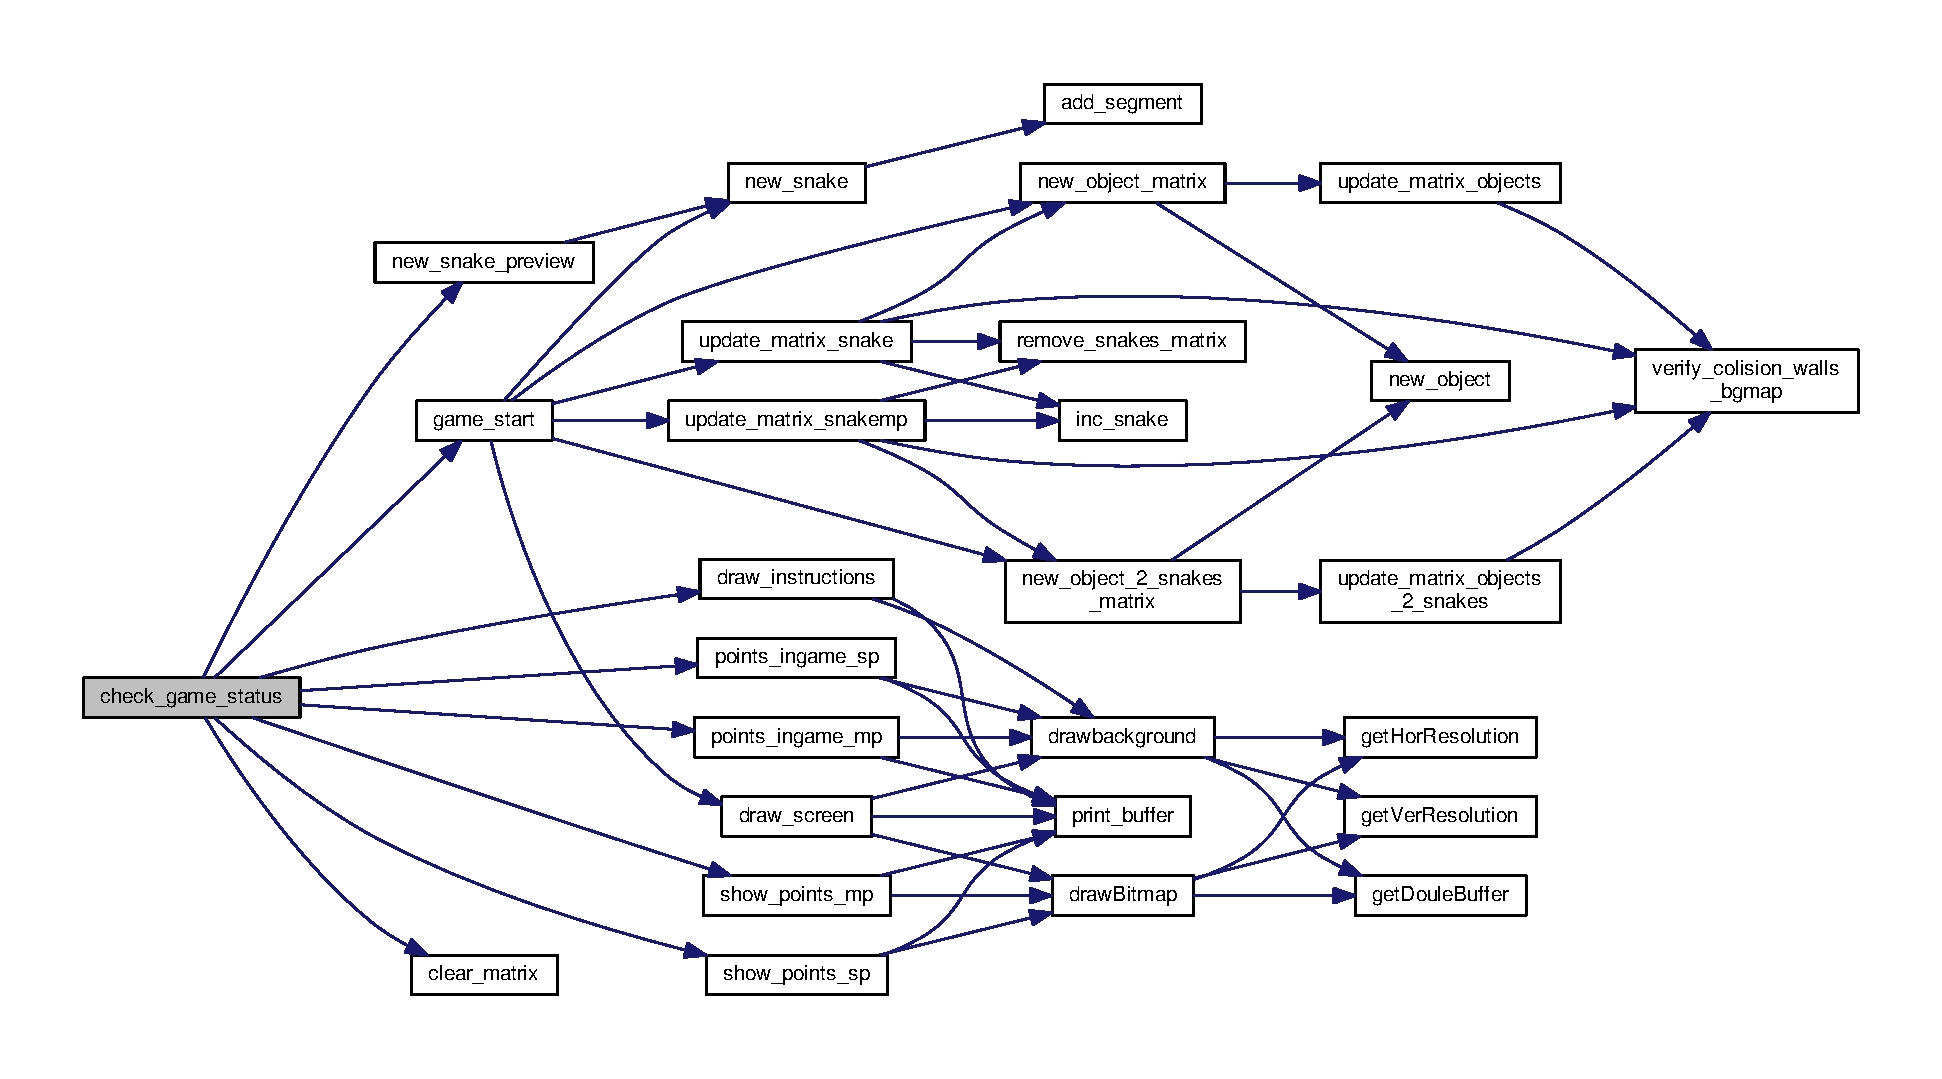
\includegraphics[width=350pt]{group__man__events_ga35641febfec789ab3ddc031482a80ea1_cgraph}
\end{center}
\end{figure}


\index{man\+\_\+events@{man\+\_\+events}!game\+\_\+start@{game\+\_\+start}}
\index{game\+\_\+start@{game\+\_\+start}!man\+\_\+events@{man\+\_\+events}}
\subsubsection[{\texorpdfstring{game\+\_\+start(int mode)}{game_start(int mode)}}]{\setlength{\rightskip}{0pt plus 5cm}void game\+\_\+start (
\begin{DoxyParamCaption}
\item[{int}]{mode}
\end{DoxyParamCaption}
)}\hypertarget{group__man__events_ga07dc5293a915fb3c924067ef41f08d23}{}\label{group__man__events_ga07dc5293a915fb3c924067ef41f08d23}


it makes the necessary actions to start a game mode (established by the parameter), create snake(s), put them in the matrix,add the initial objects,etc 


\begin{DoxyParams}{Parameters}
{\em mode} & simple number to identify the game mode that is going to start\\
\hline
\end{DoxyParams}
If mode is equal to 1 the function is going to make the preparations to the singleplayer mode If mode is equal to 2 the function is going to make the preparations to the multiplayer, 2 snakes mode If mode is equal to 3 the function is going to make the preparations to the multiplayer with mouse mode 

Here is the call graph for this function\+:
\nopagebreak
\begin{figure}[H]
\begin{center}
\leavevmode
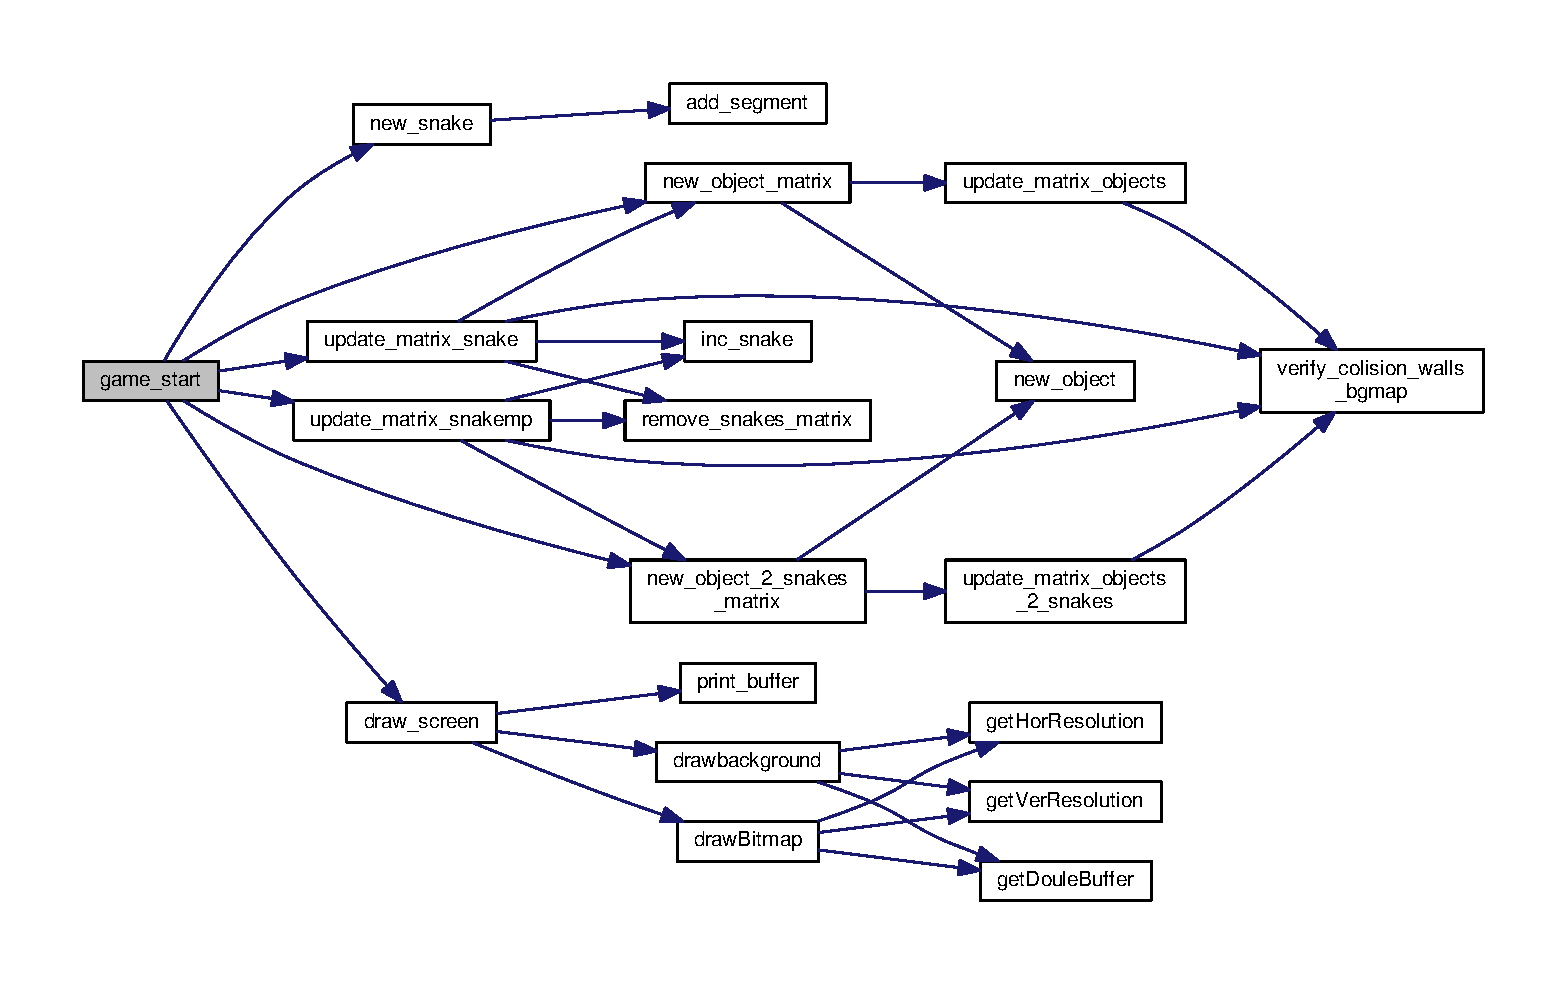
\includegraphics[width=350pt]{group__man__events_ga07dc5293a915fb3c924067ef41f08d23_cgraph}
\end{center}
\end{figure}


\index{man\+\_\+events@{man\+\_\+events}!keyboard\+\_\+event\+\_\+handler@{keyboard\+\_\+event\+\_\+handler}}
\index{keyboard\+\_\+event\+\_\+handler@{keyboard\+\_\+event\+\_\+handler}!man\+\_\+events@{man\+\_\+events}}
\subsubsection[{\texorpdfstring{keyboard\+\_\+event\+\_\+handler(unsigned long out\+\_\+buf)}{keyboard_event_handler(unsigned long out_buf)}}]{\setlength{\rightskip}{0pt plus 5cm}int keyboard\+\_\+event\+\_\+handler (
\begin{DoxyParamCaption}
\item[{unsigned long}]{out\+\_\+buf}
\end{DoxyParamCaption}
)}\hypertarget{group__man__events_ga87d21261b5adc5a0dccb151f938735a9}{}\label{group__man__events_ga87d21261b5adc5a0dccb151f938735a9}


it interprets the interrupts of the keyboard and \char`\"{}acts\char`\"{} if the keys are pressed in the necessary states 


\begin{DoxyParams}{Parameters}
{\em out\+\_\+buf} & the code of the key pressed (it works with codes of 2 Bytes) \\
\hline
\end{DoxyParams}


Here is the call graph for this function\+:
\nopagebreak
\begin{figure}[H]
\begin{center}
\leavevmode
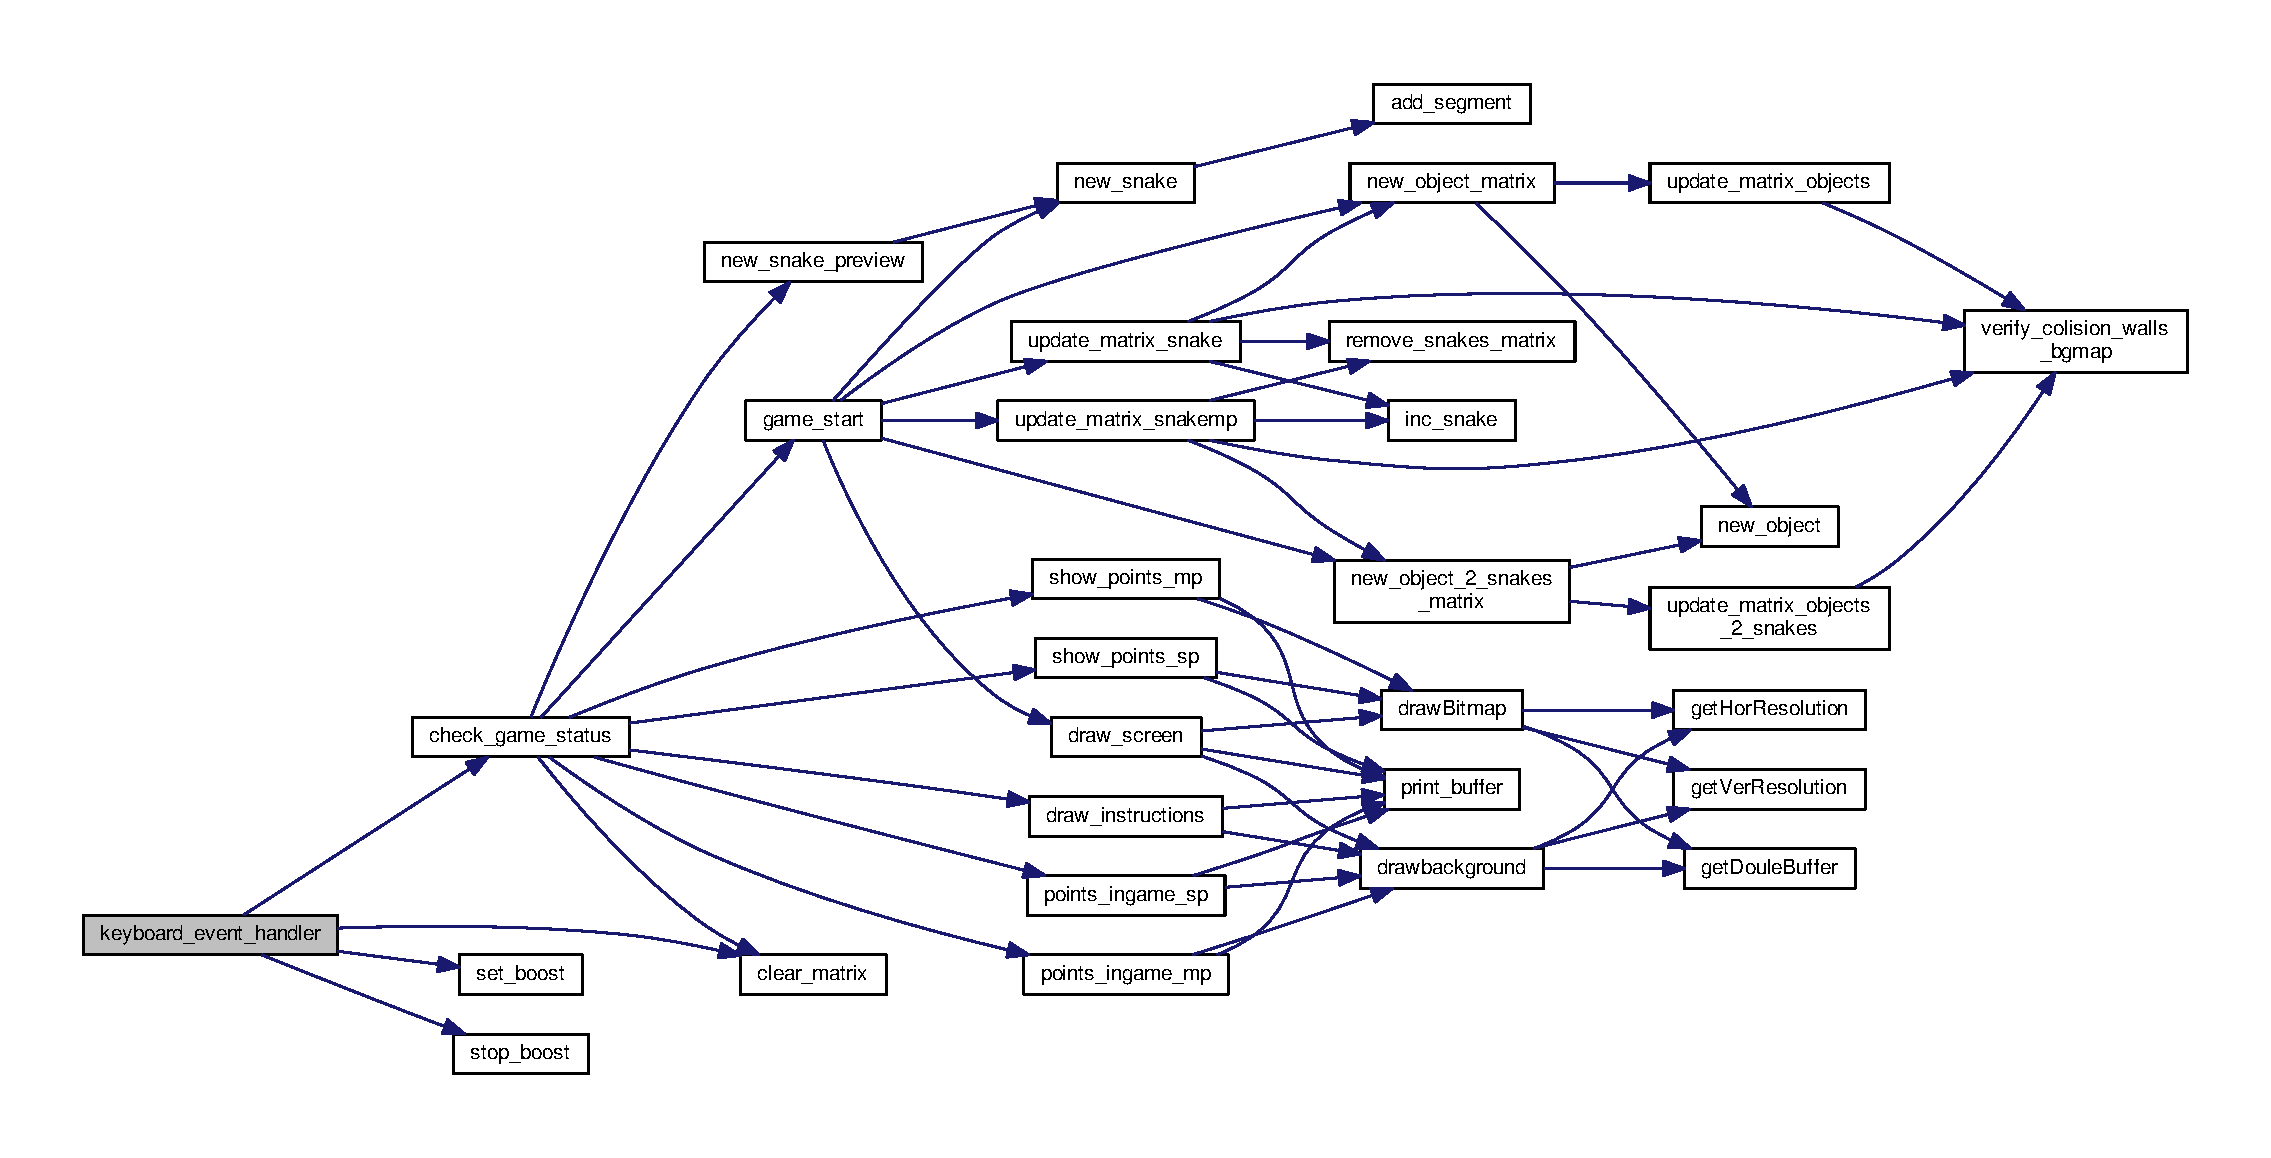
\includegraphics[width=350pt]{group__man__events_ga87d21261b5adc5a0dccb151f938735a9_cgraph}
\end{center}
\end{figure}


\index{man\+\_\+events@{man\+\_\+events}!mouse\+\_\+event\+\_\+handler@{mouse\+\_\+event\+\_\+handler}}
\index{mouse\+\_\+event\+\_\+handler@{mouse\+\_\+event\+\_\+handler}!man\+\_\+events@{man\+\_\+events}}
\subsubsection[{\texorpdfstring{mouse\+\_\+event\+\_\+handler(unsigned long $\ast$packet\+\_\+mouse)}{mouse_event_handler(unsigned long *packet_mouse)}}]{\setlength{\rightskip}{0pt plus 5cm}void mouse\+\_\+event\+\_\+handler (
\begin{DoxyParamCaption}
\item[{unsigned long $\ast$}]{packet\+\_\+mouse}
\end{DoxyParamCaption}
)}\hypertarget{group__man__events_ga9c2df329e13887f8f241315c35057d77}{}\label{group__man__events_ga9c2df329e13887f8f241315c35057d77}


in interprets the interrupts of the mouse and acts depending of the currently state of the state machine 


\begin{DoxyParams}{Parameters}
{\em packet\+\_\+mouse} & the mouse packet that is useful to know the position of the mouse and the buttons that are pressed \\
\hline
\end{DoxyParams}


Here is the call graph for this function\+:
\nopagebreak
\begin{figure}[H]
\begin{center}
\leavevmode
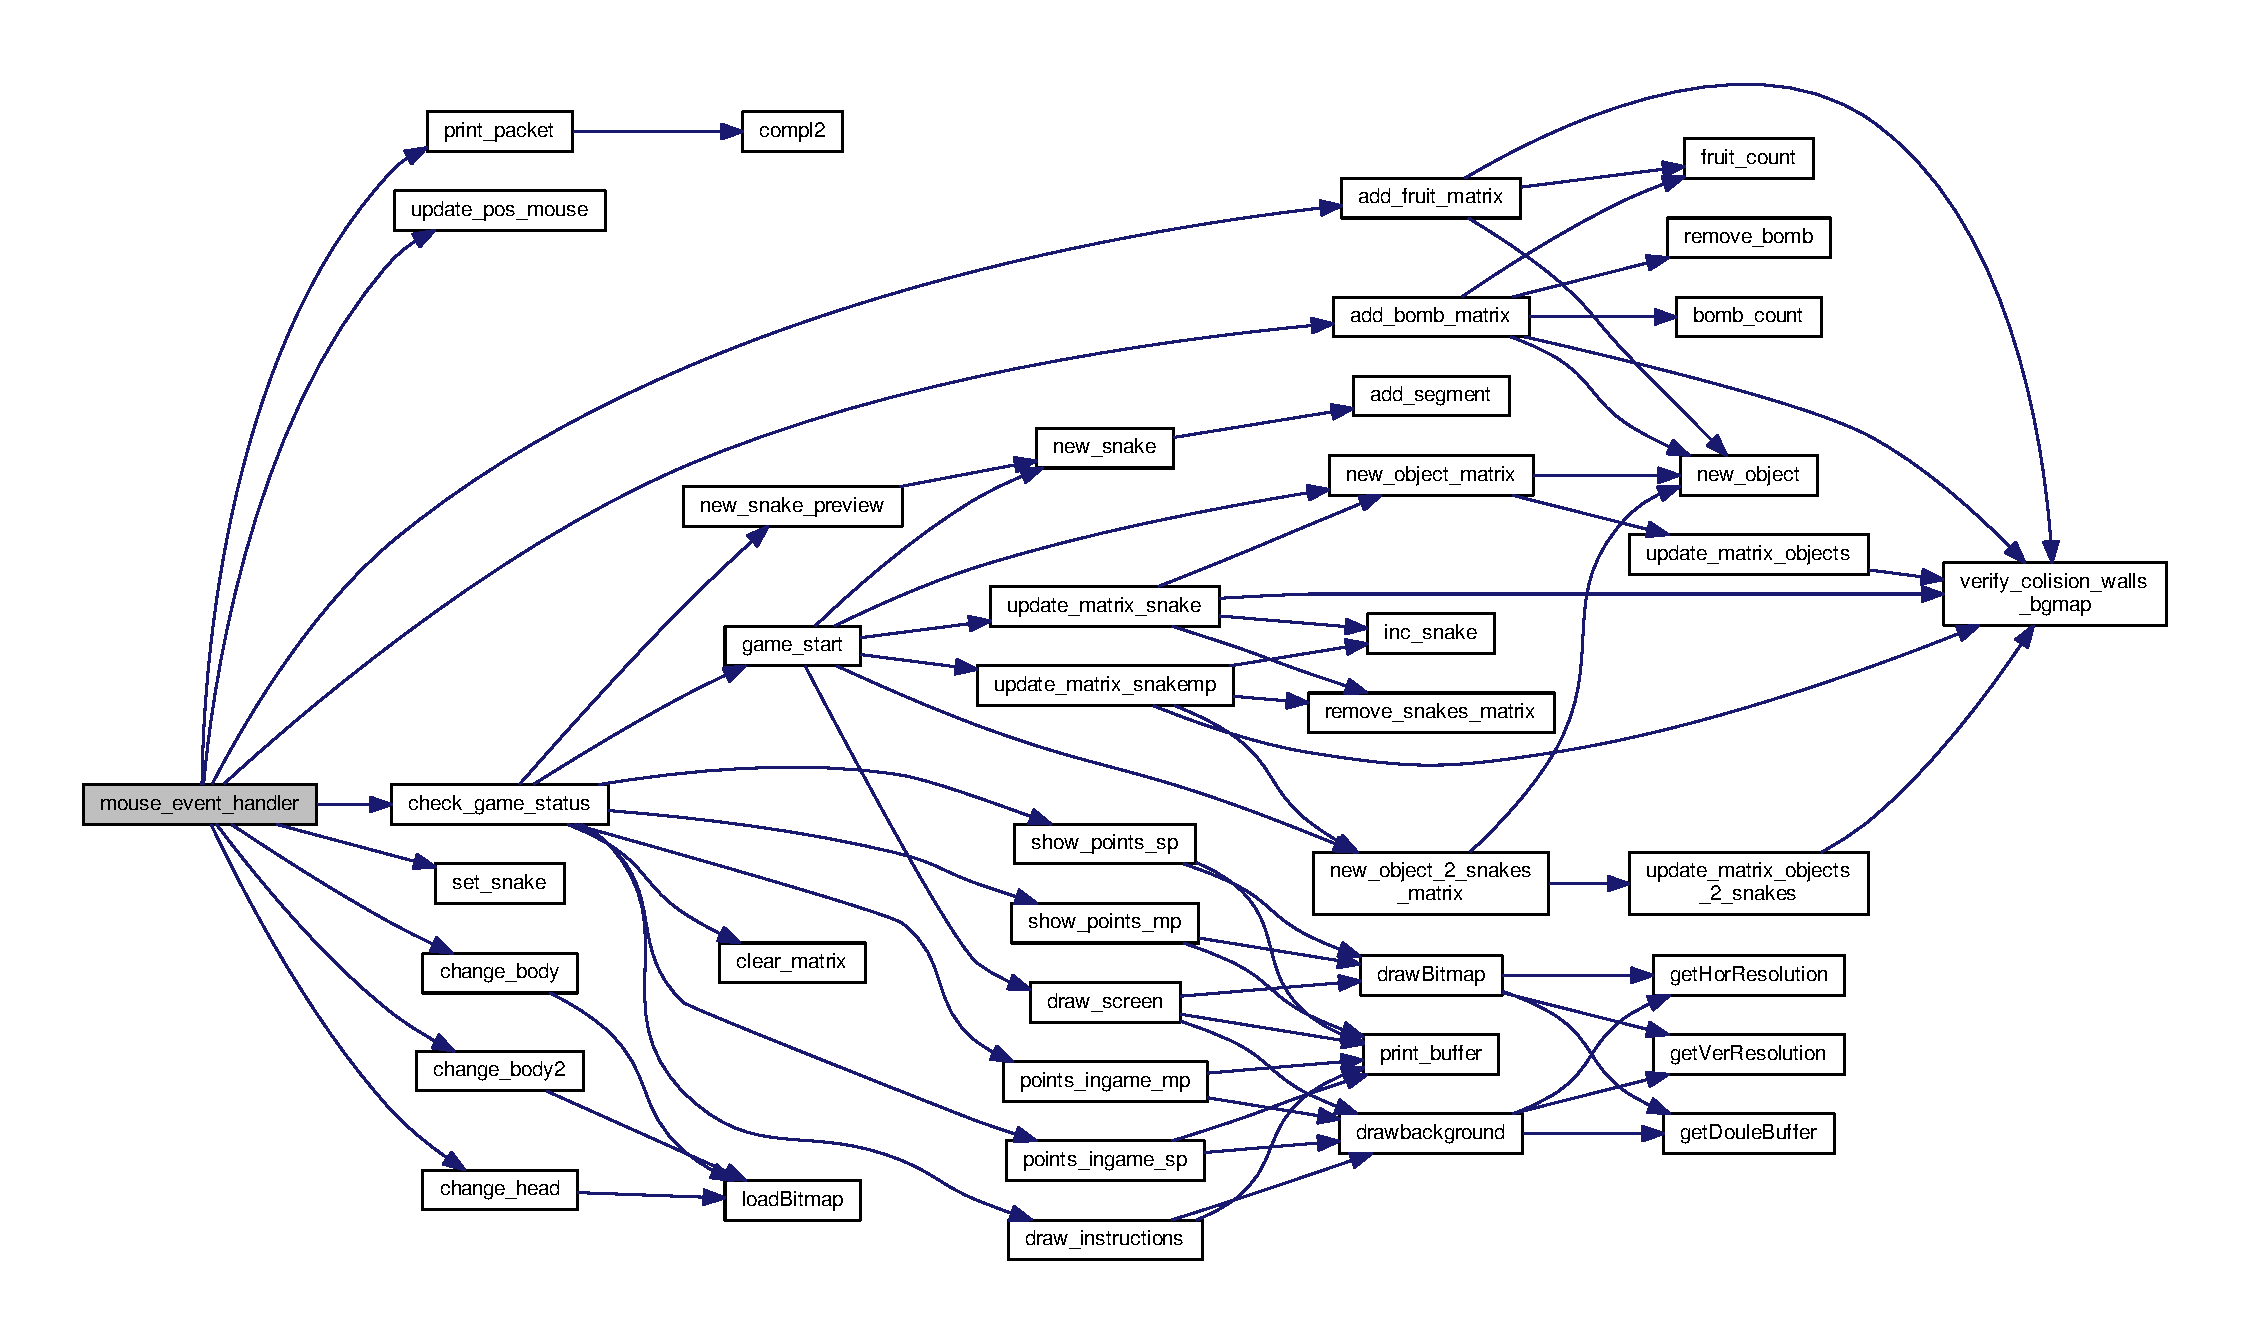
\includegraphics[width=350pt]{group__man__events_ga9c2df329e13887f8f241315c35057d77_cgraph}
\end{center}
\end{figure}


\index{man\+\_\+events@{man\+\_\+events}!new\+\_\+snake\+\_\+preview@{new\+\_\+snake\+\_\+preview}}
\index{new\+\_\+snake\+\_\+preview@{new\+\_\+snake\+\_\+preview}!man\+\_\+events@{man\+\_\+events}}
\subsubsection[{\texorpdfstring{new\+\_\+snake\+\_\+preview()}{new_snake_preview()}}]{\setlength{\rightskip}{0pt plus 5cm}void new\+\_\+snake\+\_\+preview (
\begin{DoxyParamCaption}
{}
\end{DoxyParamCaption}
)}\hypertarget{group__man__events_gacc914291496b74fddbe876393dda69a6}{}\label{group__man__events_gacc914291496b74fddbe876393dda69a6}


creates the snake that is shown in the choose skin of the snake menu before each game 



Here is the call graph for this function\+:
\nopagebreak
\begin{figure}[H]
\begin{center}
\leavevmode
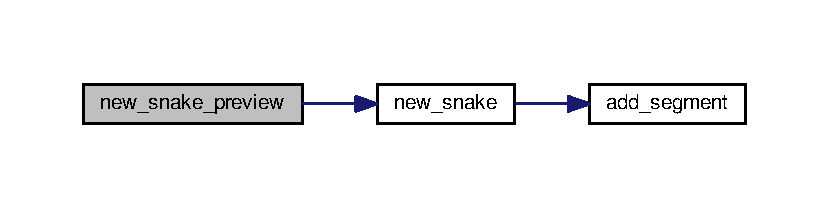
\includegraphics[width=350pt]{group__man__events_gacc914291496b74fddbe876393dda69a6_cgraph}
\end{center}
\end{figure}


\index{man\+\_\+events@{man\+\_\+events}!timer\+\_\+event\+\_\+handler@{timer\+\_\+event\+\_\+handler}}
\index{timer\+\_\+event\+\_\+handler@{timer\+\_\+event\+\_\+handler}!man\+\_\+events@{man\+\_\+events}}
\subsubsection[{\texorpdfstring{timer\+\_\+event\+\_\+handler(unsigned short counter)}{timer_event_handler(unsigned short counter)}}]{\setlength{\rightskip}{0pt plus 5cm}int timer\+\_\+event\+\_\+handler (
\begin{DoxyParamCaption}
\item[{unsigned short}]{counter}
\end{DoxyParamCaption}
)}\hypertarget{group__man__events_ga5c998385f8d5e28e1380654ad355e0b5}{}\label{group__man__events_ga5c998385f8d5e28e1380654ad355e0b5}


it interprets the interrupts of the timer and acts differently depending of the state that the state machine is currently in 


\begin{DoxyParams}{Parameters}
{\em counter} & of the interrupt handler \\
\hline
\end{DoxyParams}


Here is the call graph for this function\+:
\nopagebreak
\begin{figure}[H]
\begin{center}
\leavevmode
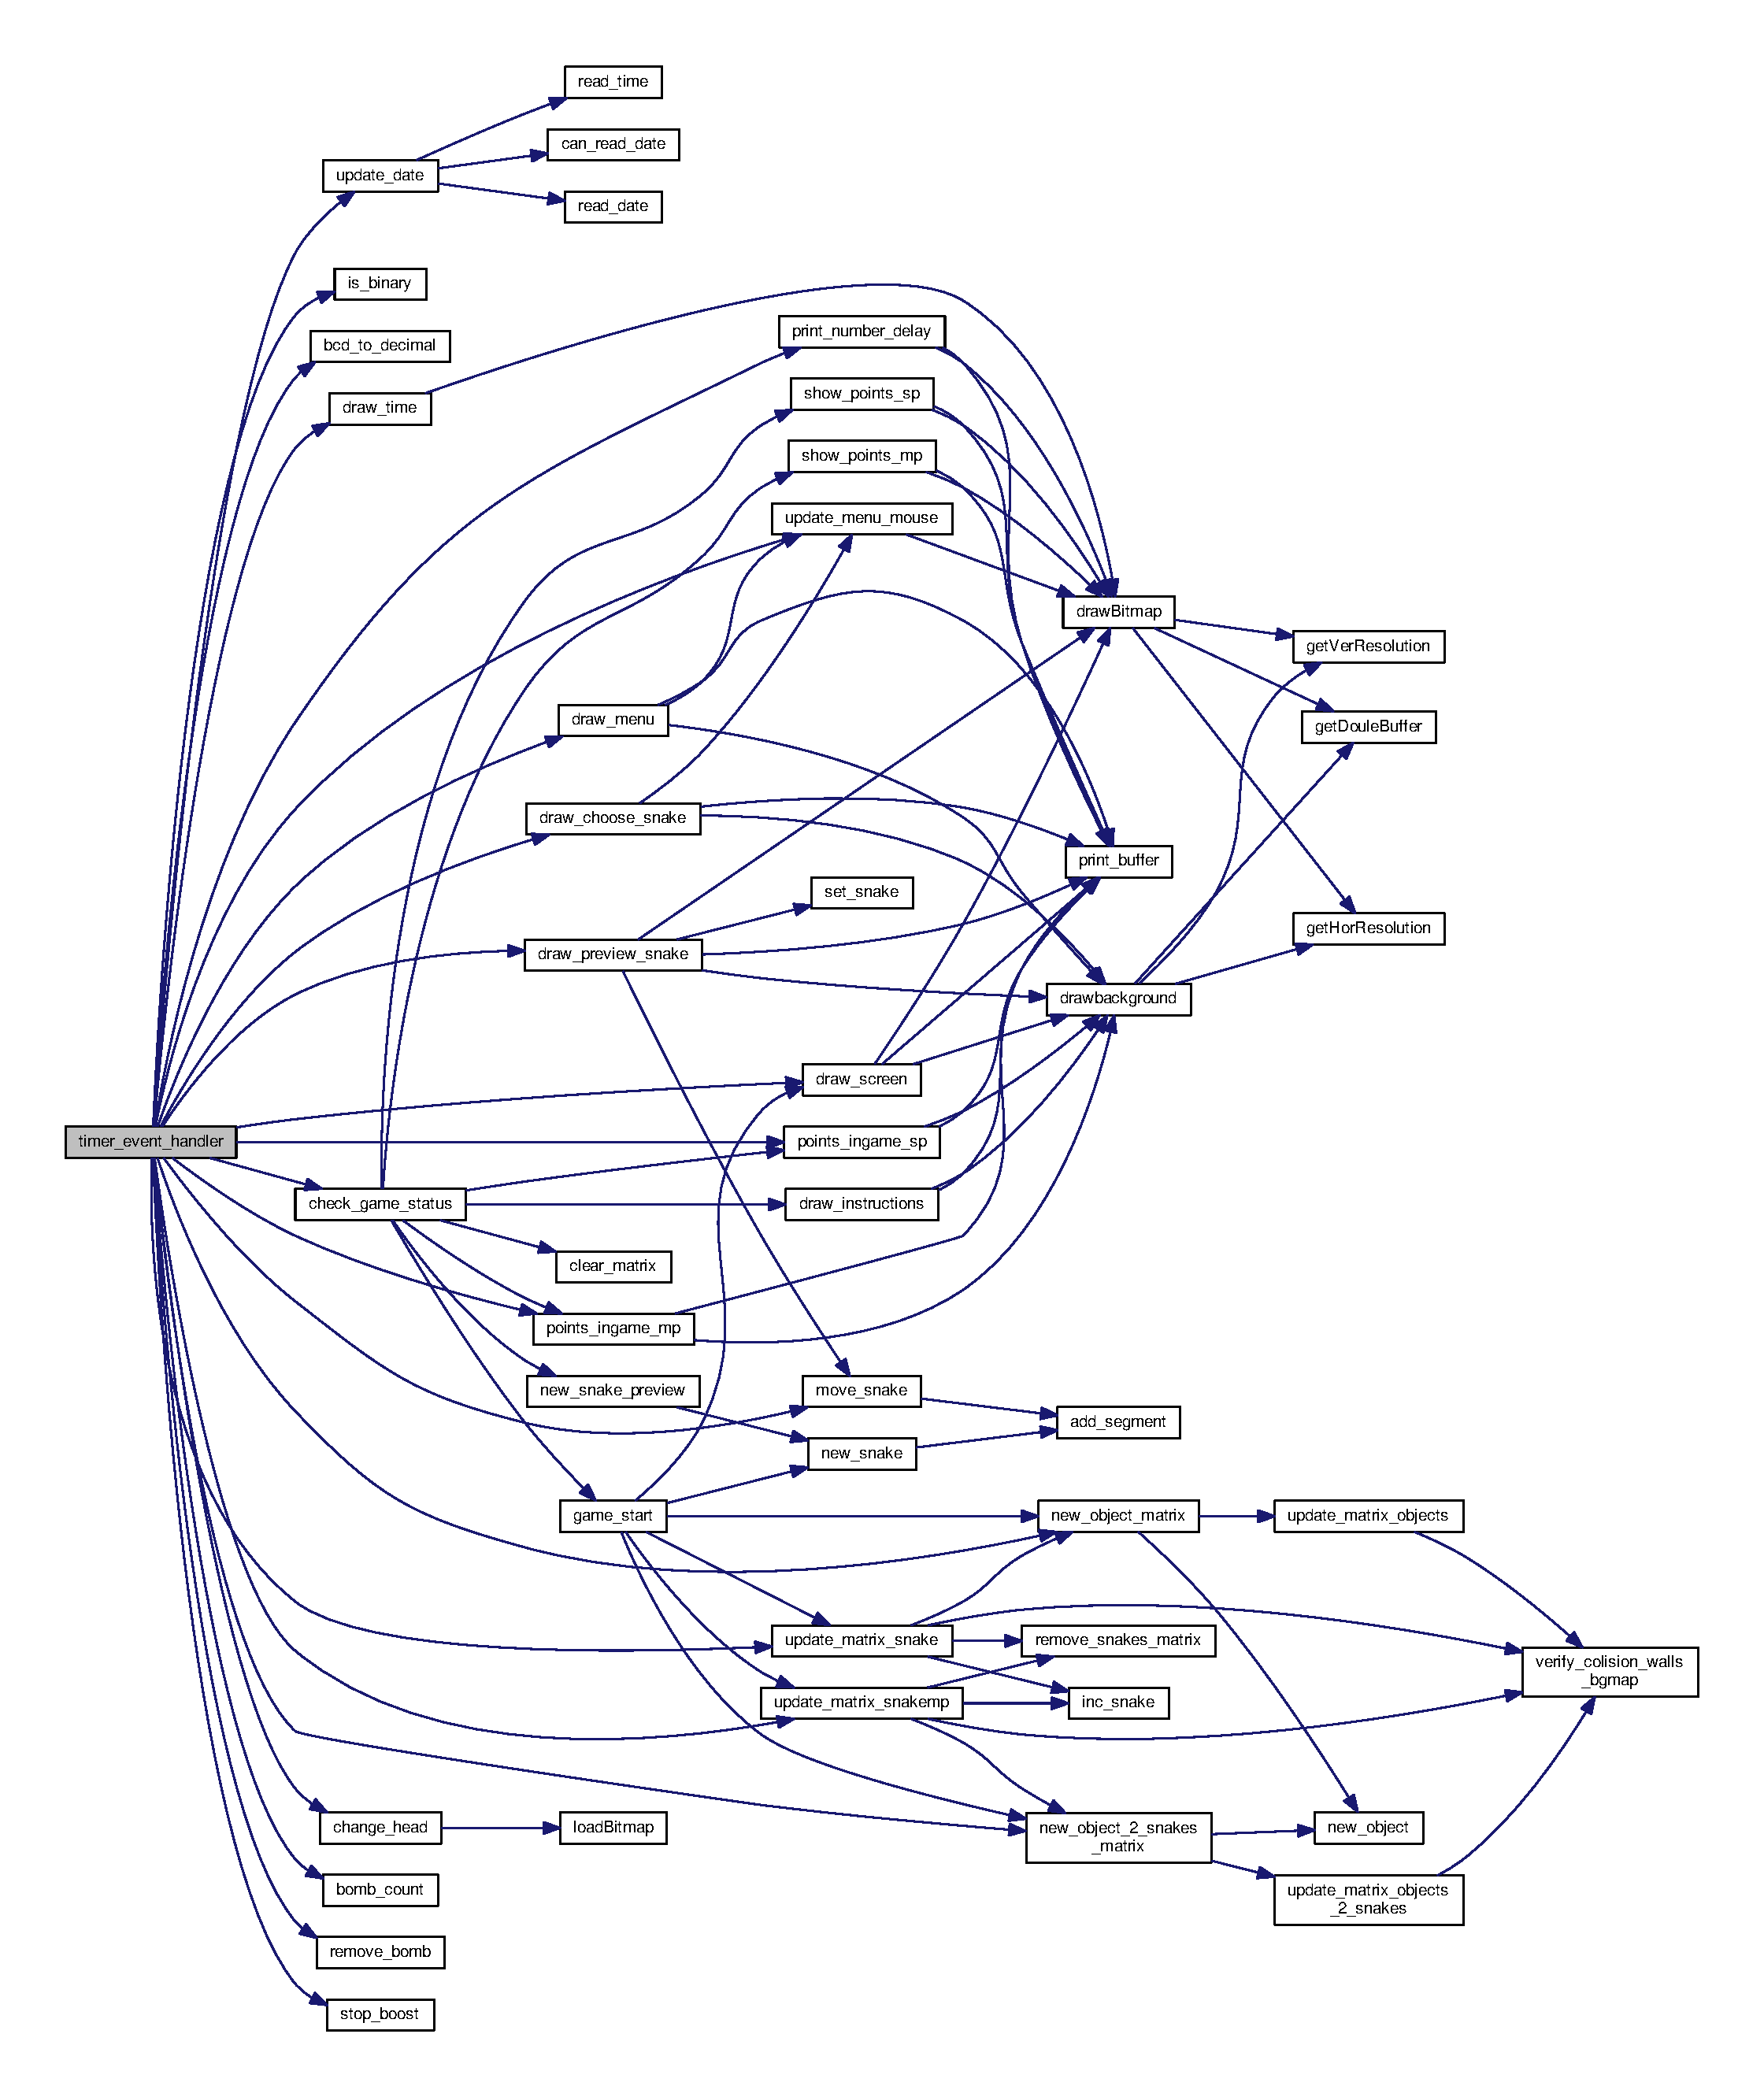
\includegraphics[width=350pt]{group__man__events_ga5c998385f8d5e28e1380654ad355e0b5_cgraph}
\end{center}
\end{figure}




\subsection{Variable Documentation}
\index{man\+\_\+events@{man\+\_\+events}!body\+\_\+flag@{body\+\_\+flag}}
\index{body\+\_\+flag@{body\+\_\+flag}!man\+\_\+events@{man\+\_\+events}}
\subsubsection[{\texorpdfstring{body\+\_\+flag}{body_flag}}]{\setlength{\rightskip}{0pt plus 5cm}int body\+\_\+flag = 0\hspace{0.3cm}{\ttfamily [static]}}\hypertarget{group__man__events_ga50e9227ad82eba24c0fa3bc0fa3c4c94}{}\label{group__man__events_ga50e9227ad82eba24c0fa3bc0fa3c4c94}
Flag to know if a body has been chosen in the choose the body menu before each game \index{man\+\_\+events@{man\+\_\+events}!buf\+\_\+full@{buf\+\_\+full}}
\index{buf\+\_\+full@{buf\+\_\+full}!man\+\_\+events@{man\+\_\+events}}
\subsubsection[{\texorpdfstring{buf\+\_\+full}{buf_full}}]{\setlength{\rightskip}{0pt plus 5cm}int buf\+\_\+full =0\hspace{0.3cm}{\ttfamily [static]}}\hypertarget{group__man__events_ga45b2c3de13c3743778747ed17bd97be6}{}\label{group__man__events_ga45b2c3de13c3743778747ed17bd97be6}
Flag to know if buffer is full \index{man\+\_\+events@{man\+\_\+events}!choose@{choose}}
\index{choose@{choose}!man\+\_\+events@{man\+\_\+events}}
\subsubsection[{\texorpdfstring{choose}{choose}}]{\setlength{\rightskip}{0pt plus 5cm}int choose = 0\hspace{0.3cm}{\ttfamily [static]}}\hypertarget{group__man__events_ga382290cee9798b0d650c1f2fb55de1d4}{}\label{group__man__events_ga382290cee9798b0d650c1f2fb55de1d4}
Flag used in multiplayer with 2 snakes to know wich snake is being changed in the choose the body menu \index{man\+\_\+events@{man\+\_\+events}!choose1@{choose1}}
\index{choose1@{choose1}!man\+\_\+events@{man\+\_\+events}}
\subsubsection[{\texorpdfstring{choose1}{choose1}}]{\setlength{\rightskip}{0pt plus 5cm}int choose1 = 0\hspace{0.3cm}{\ttfamily [static]}}\hypertarget{group__man__events_ga11ede57042994849c9753d651a6c31f0}{}\label{group__man__events_ga11ede57042994849c9753d651a6c31f0}
Variable to make sure that in the 2 snakes mode, the same body isnt chosen for both snakes \index{man\+\_\+events@{man\+\_\+events}!date@{date}}
\index{date@{date}!man\+\_\+events@{man\+\_\+events}}
\subsubsection[{\texorpdfstring{date}{date}}]{\setlength{\rightskip}{0pt plus 5cm}{\bf date\+\_\+rtc} date}\hypertarget{group__man__events_gaa68c2949762722dfdaa5fa0e70d23cec}{}\label{group__man__events_gaa68c2949762722dfdaa5fa0e70d23cec}
time of the system \index{man\+\_\+events@{man\+\_\+events}!flag\+\_\+colision@{flag\+\_\+colision}}
\index{flag\+\_\+colision@{flag\+\_\+colision}!man\+\_\+events@{man\+\_\+events}}
\subsubsection[{\texorpdfstring{flag\+\_\+colision}{flag_colision}}]{\setlength{\rightskip}{0pt plus 5cm}int flag\+\_\+colision = 0\hspace{0.3cm}{\ttfamily [static]}}\hypertarget{group__man__events_ga4cf8437a340f1c3bc00642b3f4fb96ae}{}\label{group__man__events_ga4cf8437a340f1c3bc00642b3f4fb96ae}
Flag to know if snake s1 as collided with something(wall or bomb) \index{man\+\_\+events@{man\+\_\+events}!flag\+\_\+colision2@{flag\+\_\+colision2}}
\index{flag\+\_\+colision2@{flag\+\_\+colision2}!man\+\_\+events@{man\+\_\+events}}
\subsubsection[{\texorpdfstring{flag\+\_\+colision2}{flag_colision2}}]{\setlength{\rightskip}{0pt plus 5cm}int flag\+\_\+colision2 = 0\hspace{0.3cm}{\ttfamily [static]}}\hypertarget{group__man__events_ga85f22d2e2394a6cf3a343f1140068ea4}{}\label{group__man__events_ga85f22d2e2394a6cf3a343f1140068ea4}
Flag to know if snake s2 as collided with something(wall or bomb) \index{man\+\_\+events@{man\+\_\+events}!head\+\_\+flag@{head\+\_\+flag}}
\index{head\+\_\+flag@{head\+\_\+flag}!man\+\_\+events@{man\+\_\+events}}
\subsubsection[{\texorpdfstring{head\+\_\+flag}{head_flag}}]{\setlength{\rightskip}{0pt plus 5cm}int head\+\_\+flag = 0\hspace{0.3cm}{\ttfamily [static]}}\hypertarget{group__man__events_ga2112e7f4b28f5bc73cc834ef6e7d97e1}{}\label{group__man__events_ga2112e7f4b28f5bc73cc834ef6e7d97e1}
Flag to know if a head has been chosen in the choose the body menu before each game \index{man\+\_\+events@{man\+\_\+events}!number\+\_\+delay@{number\+\_\+delay}}
\index{number\+\_\+delay@{number\+\_\+delay}!man\+\_\+events@{man\+\_\+events}}
\subsubsection[{\texorpdfstring{number\+\_\+delay}{number_delay}}]{\setlength{\rightskip}{0pt plus 5cm}int number\+\_\+delay =3\hspace{0.3cm}{\ttfamily [static]}}\hypertarget{group__man__events_ga49dac5534222e1641ae32eba8e7baf8e}{}\label{group__man__events_ga49dac5534222e1641ae32eba8e7baf8e}
Global counter to set 3 seconds before every game starts \index{man\+\_\+events@{man\+\_\+events}!p@{p}}
\index{p@{p}!man\+\_\+events@{man\+\_\+events}}
\subsubsection[{\texorpdfstring{p}{p}}]{\setlength{\rightskip}{0pt plus 5cm}{\bf states} p ={\bf M\+E\+N\+U\+\_\+T}\hspace{0.3cm}{\ttfamily [static]}}\hypertarget{group__man__events_ga70c7b8b5ec6a67ce08a8b74a970b88fa}{}\label{group__man__events_ga70c7b8b5ec6a67ce08a8b74a970b88fa}
\index{man\+\_\+events@{man\+\_\+events}!s1@{s1}}
\index{s1@{s1}!man\+\_\+events@{man\+\_\+events}}
\subsubsection[{\texorpdfstring{s1}{s1}}]{\setlength{\rightskip}{0pt plus 5cm}{\bf Snake}$\ast$ s1\hspace{0.3cm}{\ttfamily [static]}}\hypertarget{group__man__events_gaf79c0d77b0cca9ebf96bbbed1f88aed0}{}\label{group__man__events_gaf79c0d77b0cca9ebf96bbbed1f88aed0}
\hyperlink{structSnake}{Snake} created used for all game modes \index{man\+\_\+events@{man\+\_\+events}!s2@{s2}}
\index{s2@{s2}!man\+\_\+events@{man\+\_\+events}}
\subsubsection[{\texorpdfstring{s2}{s2}}]{\setlength{\rightskip}{0pt plus 5cm}{\bf Snake}$\ast$ s2\hspace{0.3cm}{\ttfamily [static]}}\hypertarget{group__man__events_ga5b853e8b22f27ef547e5b45e4197d308}{}\label{group__man__events_ga5b853e8b22f27ef547e5b45e4197d308}
\hyperlink{structSnake}{Snake} created used for all the multiplayer modes \index{man\+\_\+events@{man\+\_\+events}!s\+\_\+preview@{s\+\_\+preview}}
\index{s\+\_\+preview@{s\+\_\+preview}!man\+\_\+events@{man\+\_\+events}}
\subsubsection[{\texorpdfstring{s\+\_\+preview}{s_preview}}]{\setlength{\rightskip}{0pt plus 5cm}{\bf Snake}$\ast$ s\+\_\+preview\hspace{0.3cm}{\ttfamily [static]}}\hypertarget{group__man__events_gad4cd59e08d196fdec29b274d2f27254b}{}\label{group__man__events_gad4cd59e08d196fdec29b274d2f27254b}
\hyperlink{structSnake}{Snake} created to preview the chosen in the choose the body of the snake menu before every game \index{man\+\_\+events@{man\+\_\+events}!second\+\_\+snake@{second\+\_\+snake}}
\index{second\+\_\+snake@{second\+\_\+snake}!man\+\_\+events@{man\+\_\+events}}
\subsubsection[{\texorpdfstring{second\+\_\+snake}{second_snake}}]{\setlength{\rightskip}{0pt plus 5cm}int second\+\_\+snake = 0\hspace{0.3cm}{\ttfamily [static]}}\hypertarget{group__man__events_ga559fc485a85afead1ca991d70e7c72ee}{}\label{group__man__events_ga559fc485a85afead1ca991d70e7c72ee}
Flag to know if it has to make the second round of the multiplayer with mouse mode \index{man\+\_\+events@{man\+\_\+events}!snakes\+\_\+mp\+\_\+modify@{snakes\+\_\+mp\+\_\+modify}}
\index{snakes\+\_\+mp\+\_\+modify@{snakes\+\_\+mp\+\_\+modify}!man\+\_\+events@{man\+\_\+events}}
\subsubsection[{\texorpdfstring{snakes\+\_\+mp\+\_\+modify}{snakes_mp_modify}}]{\setlength{\rightskip}{0pt plus 5cm}int snakes\+\_\+mp\+\_\+modify =0\hspace{0.3cm}{\ttfamily [static]}}\hypertarget{group__man__events_ga96e3c9a348a3b68cb9b715a021eb8005}{}\label{group__man__events_ga96e3c9a348a3b68cb9b715a021eb8005}
\index{man\+\_\+events@{man\+\_\+events}!t@{t}}
\index{t@{t}!man\+\_\+events@{man\+\_\+events}}
\subsubsection[{\texorpdfstring{t}{t}}]{\setlength{\rightskip}{0pt plus 5cm}{\bf event} t}\hypertarget{group__man__events_gac7f56a32062f381248ce9a81e701ff8a}{}\label{group__man__events_gac7f56a32062f381248ce9a81e701ff8a}

\hypertarget{group__menu}{}\section{menu}
\label{group__menu}\index{menu@{menu}}
\subsection*{Functions}
\begin{DoxyCompactItemize}
\item 
void \hyperlink{group__menu_gaa00e45cbd295e588746a7f2fd88b0d20}{start\+\_\+variables\+\_\+menu} ()
\begin{DoxyCompactList}\small\item\em it fills the bmp global variable with the bitmaps loaded in \hyperlink{graphics_8c}{graphics.\+c} \end{DoxyCompactList}\item 
void \hyperlink{group__menu_gab149955bb30c6e7a2923c73e86c09ac9}{update\+\_\+pos\+\_\+mouse} (unsigned long $\ast$x, unsigned long $\ast$y)
\begin{DoxyCompactList}\small\item\em it updates the x\+\_\+pos\+\_\+atual and y\+\_\+pos\+\_\+atual of the mouse \end{DoxyCompactList}\item 
void \hyperlink{group__menu_ga937fb72019d190110b15fdf01d17992b}{draw\+\_\+menu} (int mode)
\begin{DoxyCompactList}\small\item\em draws in the screen the menu specified \end{DoxyCompactList}\item 
void \hyperlink{group__menu_gab1b3c1e3e90e9c78f31cddcc2544fd09}{update\+\_\+menu\+\_\+mouse} ()
\begin{DoxyCompactList}\small\item\em draws in the screen the mouse cursor in the current position of the mouse \end{DoxyCompactList}\item 
void \hyperlink{group__menu_ga95721c20a1fd0be4884cd0a0f8168f53}{change\+\_\+body} (int opt)
\begin{DoxyCompactList}\small\item\em it changes the bmp associated with the variable body \end{DoxyCompactList}\item 
void \hyperlink{group__menu_ga8f65ea2dd45c3b01b9f3752fc04745db}{change\+\_\+body2} (int opt)
\begin{DoxyCompactList}\small\item\em it changes the bmp associated with the variable body2 \end{DoxyCompactList}\item 
void \hyperlink{group__menu_ga0c2bebb094507763ab9c3343f554c0cc}{change\+\_\+head} (int opt)
\begin{DoxyCompactList}\small\item\em it changes all the bmps associated with the variables of the head of snake s1 \end{DoxyCompactList}\item 
void \hyperlink{group__menu_gafebc2d04c898f861176790d50232e001}{draw\+\_\+choose\+\_\+snake} (int mode)
\begin{DoxyCompactList}\small\item\em draws the menus to choose the body of the snakes \end{DoxyCompactList}\item 
void \hyperlink{group__menu_ga75fa9eba2da71d7eafa82e469cf35053}{draw\+\_\+preview\+\_\+snake} (\hyperlink{structSnake}{Snake} $\ast$snake\+\_\+preview, int counter, int body\+\_\+count)
\begin{DoxyCompactList}\small\item\em draws in any of the choose menus a preview snake to see how the options chosen looks \end{DoxyCompactList}\item 
void \hyperlink{group__menu_ga9b565fa7246d14c851c7d66b487e21fc}{draw\+\_\+time} (int hour, int min, int seconds)
\begin{DoxyCompactList}\small\item\em it draws in the menus the current time of the system \end{DoxyCompactList}\item 
void \hyperlink{group__menu_ga4a36c7e8b7af7e8f586a739cd54b85b4}{draw\+\_\+instructions} (int mode)
\begin{DoxyCompactList}\small\item\em draws the game instructions of each game mode \end{DoxyCompactList}\item 
void \hyperlink{group__menu_ga2cb72366439253e4818c96e350f195d2}{show\+\_\+points\+\_\+sp} (\hyperlink{structSnake}{Snake} $\ast$\hyperlink{group__man__events_gaf79c0d77b0cca9ebf96bbbed1f88aed0}{s1})
\begin{DoxyCompactList}\small\item\em show the end game points of the snake(1 snake modes) \end{DoxyCompactList}\item 
void \hyperlink{group__menu_ga1ceb0e04a7680faf9583052de831fbe6}{show\+\_\+points\+\_\+mp} (\hyperlink{structSnake}{Snake} $\ast$\hyperlink{group__man__events_gaf79c0d77b0cca9ebf96bbbed1f88aed0}{s1}, \hyperlink{structSnake}{Snake} $\ast$\hyperlink{group__man__events_ga5b853e8b22f27ef547e5b45e4197d308}{s2})
\begin{DoxyCompactList}\small\item\em show the end game points of both players snakes (2 snake modes) \end{DoxyCompactList}\end{DoxyCompactItemize}


\subsection{Detailed Description}
Functions related to the game menus 

\subsection{Function Documentation}
\index{menu@{menu}!change\+\_\+body@{change\+\_\+body}}
\index{change\+\_\+body@{change\+\_\+body}!menu@{menu}}
\subsubsection[{\texorpdfstring{change\+\_\+body(int opt)}{change_body(int opt)}}]{\setlength{\rightskip}{0pt plus 5cm}void change\+\_\+body (
\begin{DoxyParamCaption}
\item[{int}]{opt}
\end{DoxyParamCaption}
)}\hypertarget{group__menu_ga95721c20a1fd0be4884cd0a0f8168f53}{}\label{group__menu_ga95721c20a1fd0be4884cd0a0f8168f53}


it changes the bmp associated with the variable body 


\begin{DoxyParams}{Parameters}
{\em opt} & wich of the bodies is being chosen \\
\hline
\end{DoxyParams}


Here is the call graph for this function\+:
\nopagebreak
\begin{figure}[H]
\begin{center}
\leavevmode
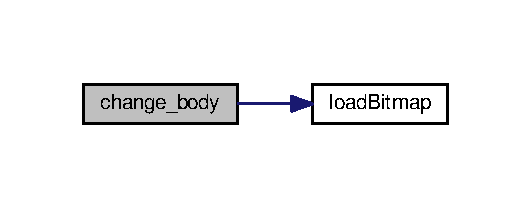
\includegraphics[width=255pt]{group__menu_ga95721c20a1fd0be4884cd0a0f8168f53_cgraph}
\end{center}
\end{figure}


\index{menu@{menu}!change\+\_\+body2@{change\+\_\+body2}}
\index{change\+\_\+body2@{change\+\_\+body2}!menu@{menu}}
\subsubsection[{\texorpdfstring{change\+\_\+body2(int opt)}{change_body2(int opt)}}]{\setlength{\rightskip}{0pt plus 5cm}void change\+\_\+body2 (
\begin{DoxyParamCaption}
\item[{int}]{opt}
\end{DoxyParamCaption}
)}\hypertarget{group__menu_ga8f65ea2dd45c3b01b9f3752fc04745db}{}\label{group__menu_ga8f65ea2dd45c3b01b9f3752fc04745db}


it changes the bmp associated with the variable body2 


\begin{DoxyParams}{Parameters}
{\em opt} & which of the bodies as been chosen \\
\hline
\end{DoxyParams}


Here is the call graph for this function\+:
\nopagebreak
\begin{figure}[H]
\begin{center}
\leavevmode
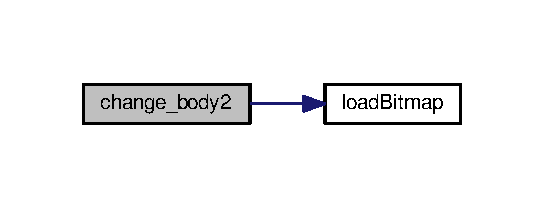
\includegraphics[width=261pt]{group__menu_ga8f65ea2dd45c3b01b9f3752fc04745db_cgraph}
\end{center}
\end{figure}


\index{menu@{menu}!change\+\_\+head@{change\+\_\+head}}
\index{change\+\_\+head@{change\+\_\+head}!menu@{menu}}
\subsubsection[{\texorpdfstring{change\+\_\+head(int opt)}{change_head(int opt)}}]{\setlength{\rightskip}{0pt plus 5cm}void change\+\_\+head (
\begin{DoxyParamCaption}
\item[{int}]{opt}
\end{DoxyParamCaption}
)}\hypertarget{group__menu_ga0c2bebb094507763ab9c3343f554c0cc}{}\label{group__menu_ga0c2bebb094507763ab9c3343f554c0cc}


it changes all the bmps associated with the variables of the head of snake s1 


\begin{DoxyParams}{Parameters}
{\em opt} & which of the heads has been chosen in the choose the body menu \\
\hline
\end{DoxyParams}


Here is the call graph for this function\+:
\nopagebreak
\begin{figure}[H]
\begin{center}
\leavevmode
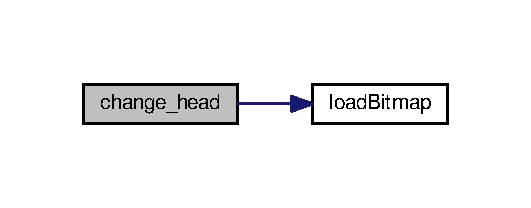
\includegraphics[width=255pt]{group__menu_ga0c2bebb094507763ab9c3343f554c0cc_cgraph}
\end{center}
\end{figure}


\index{menu@{menu}!draw\+\_\+choose\+\_\+snake@{draw\+\_\+choose\+\_\+snake}}
\index{draw\+\_\+choose\+\_\+snake@{draw\+\_\+choose\+\_\+snake}!menu@{menu}}
\subsubsection[{\texorpdfstring{draw\+\_\+choose\+\_\+snake(int mode)}{draw_choose_snake(int mode)}}]{\setlength{\rightskip}{0pt plus 5cm}void draw\+\_\+choose\+\_\+snake (
\begin{DoxyParamCaption}
\item[{int}]{mode}
\end{DoxyParamCaption}
)}\hypertarget{group__menu_gafebc2d04c898f861176790d50232e001}{}\label{group__menu_gafebc2d04c898f861176790d50232e001}


draws the menus to choose the body of the snakes 


\begin{DoxyParams}{Parameters}
{\em mode} & variabel to know which choose menu is going to draw, 1 for the menu that can change body and head of snake s1, 1 and 2 for menus to choose only the bodies of the snakes s1 and s2 respectively \\
\hline
\end{DoxyParams}


Here is the call graph for this function\+:
\nopagebreak
\begin{figure}[H]
\begin{center}
\leavevmode
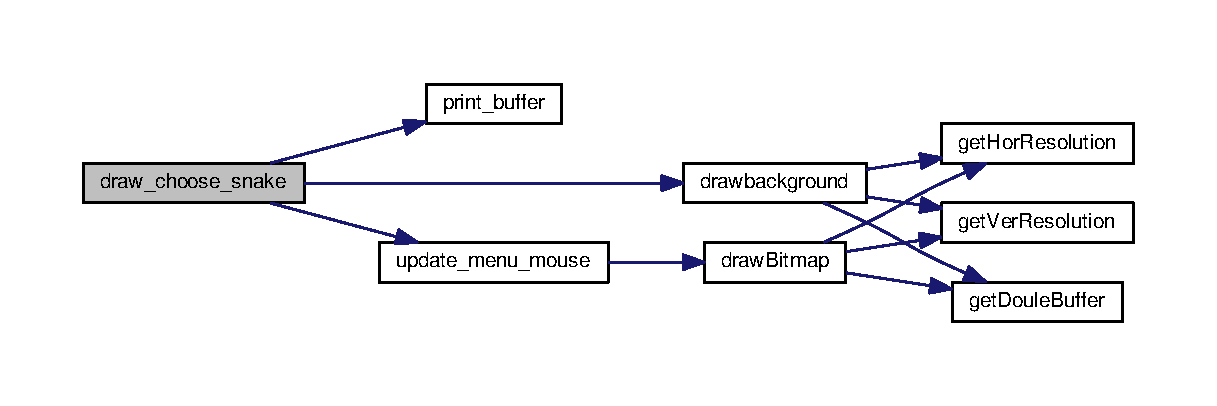
\includegraphics[width=350pt]{group__menu_gafebc2d04c898f861176790d50232e001_cgraph}
\end{center}
\end{figure}


\index{menu@{menu}!draw\+\_\+instructions@{draw\+\_\+instructions}}
\index{draw\+\_\+instructions@{draw\+\_\+instructions}!menu@{menu}}
\subsubsection[{\texorpdfstring{draw\+\_\+instructions(int mode)}{draw_instructions(int mode)}}]{\setlength{\rightskip}{0pt plus 5cm}void draw\+\_\+instructions (
\begin{DoxyParamCaption}
\item[{int}]{mode}
\end{DoxyParamCaption}
)}\hypertarget{group__menu_ga4a36c7e8b7af7e8f586a739cd54b85b4}{}\label{group__menu_ga4a36c7e8b7af7e8f586a739cd54b85b4}


draws the game instructions of each game mode 


\begin{DoxyParams}{Parameters}
{\em mode} & to know which game mode it is, 1 for singleplayer 2 for 2 snakes and 3 for the snake and mouse mode (0 is to draw the pause message when game is paused) \\
\hline
\end{DoxyParams}


Here is the call graph for this function\+:
\nopagebreak
\begin{figure}[H]
\begin{center}
\leavevmode
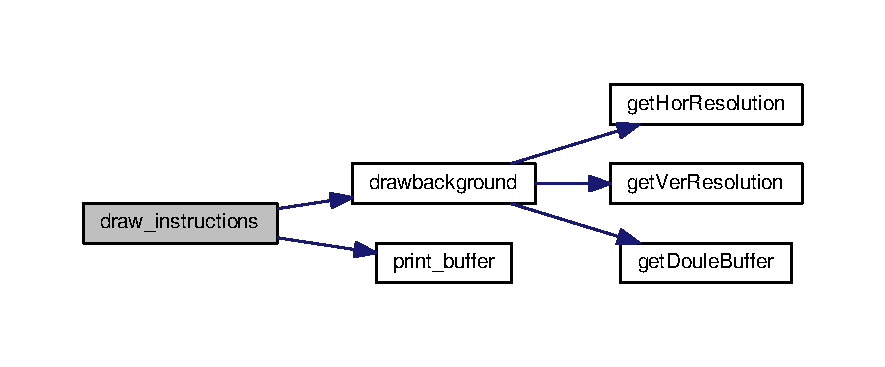
\includegraphics[width=350pt]{group__menu_ga4a36c7e8b7af7e8f586a739cd54b85b4_cgraph}
\end{center}
\end{figure}


\index{menu@{menu}!draw\+\_\+menu@{draw\+\_\+menu}}
\index{draw\+\_\+menu@{draw\+\_\+menu}!menu@{menu}}
\subsubsection[{\texorpdfstring{draw\+\_\+menu(int mode)}{draw_menu(int mode)}}]{\setlength{\rightskip}{0pt plus 5cm}void draw\+\_\+menu (
\begin{DoxyParamCaption}
\item[{int}]{mode}
\end{DoxyParamCaption}
)}\hypertarget{group__menu_ga937fb72019d190110b15fdf01d17992b}{}\label{group__menu_ga937fb72019d190110b15fdf01d17992b}


draws in the screen the menu specified 


\begin{DoxyParams}{Parameters}
{\em mode} & to know what menu is going to draw, 0 for the main menu, 1 for the multiplayer menu \\
\hline
\end{DoxyParams}


Here is the call graph for this function\+:
\nopagebreak
\begin{figure}[H]
\begin{center}
\leavevmode
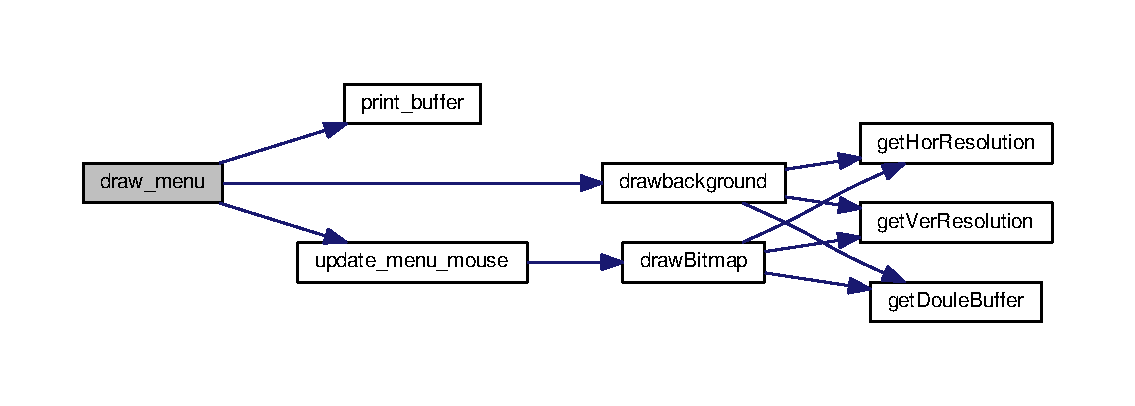
\includegraphics[width=350pt]{group__menu_ga937fb72019d190110b15fdf01d17992b_cgraph}
\end{center}
\end{figure}


\index{menu@{menu}!draw\+\_\+preview\+\_\+snake@{draw\+\_\+preview\+\_\+snake}}
\index{draw\+\_\+preview\+\_\+snake@{draw\+\_\+preview\+\_\+snake}!menu@{menu}}
\subsubsection[{\texorpdfstring{draw\+\_\+preview\+\_\+snake(\+Snake $\ast$snake\+\_\+preview, int counter, int body\+\_\+count)}{draw_preview_snake(Snake *snake_preview, int counter, int body_count)}}]{\setlength{\rightskip}{0pt plus 5cm}void draw\+\_\+preview\+\_\+snake (
\begin{DoxyParamCaption}
\item[{{\bf Snake} $\ast$}]{snake\+\_\+preview, }
\item[{int}]{counter, }
\item[{int}]{body\+\_\+count}
\end{DoxyParamCaption}
)}\hypertarget{group__menu_ga75fa9eba2da71d7eafa82e469cf35053}{}\label{group__menu_ga75fa9eba2da71d7eafa82e469cf35053}


draws in any of the choose menus a preview snake to see how the options chosen looks 


\begin{DoxyParams}{Parameters}
{\em snake\+\_\+preview} & the snake it is going to draw and move \\
\hline
{\em counter} & variable helpful to make sure if the snake is at the beggining or end of the demo \\
\hline
{\em body\+\_\+count} & variable helpful to make sure if the snake is at the beggining or end of the demo \\
\hline
\end{DoxyParams}


Here is the call graph for this function\+:
\nopagebreak
\begin{figure}[H]
\begin{center}
\leavevmode
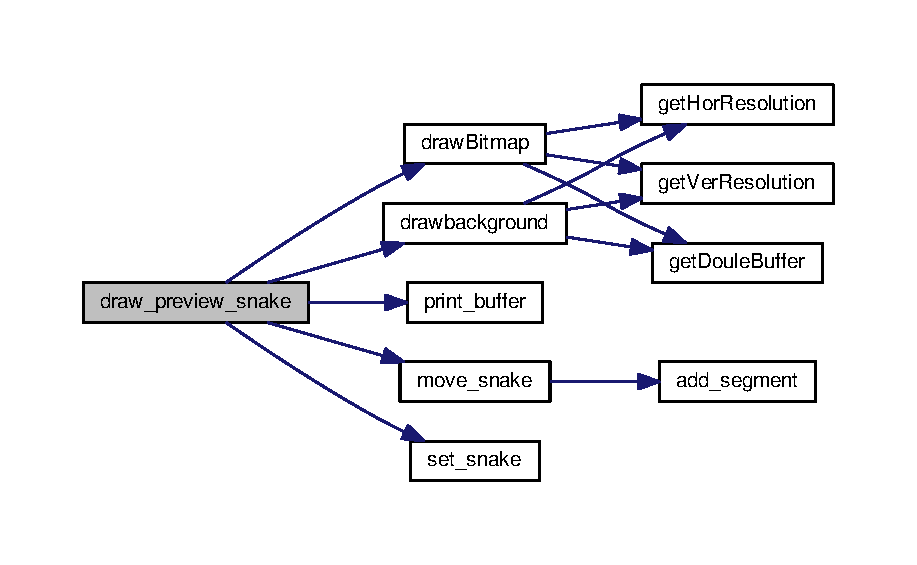
\includegraphics[width=350pt]{group__menu_ga75fa9eba2da71d7eafa82e469cf35053_cgraph}
\end{center}
\end{figure}


\index{menu@{menu}!draw\+\_\+time@{draw\+\_\+time}}
\index{draw\+\_\+time@{draw\+\_\+time}!menu@{menu}}
\subsubsection[{\texorpdfstring{draw\+\_\+time(int hour, int min, int seconds)}{draw_time(int hour, int min, int seconds)}}]{\setlength{\rightskip}{0pt plus 5cm}void draw\+\_\+time (
\begin{DoxyParamCaption}
\item[{int}]{hour, }
\item[{int}]{min, }
\item[{int}]{seconds}
\end{DoxyParamCaption}
)}\hypertarget{group__menu_ga9b565fa7246d14c851c7d66b487e21fc}{}\label{group__menu_ga9b565fa7246d14c851c7d66b487e21fc}


it draws in the menus the current time of the system 


\begin{DoxyParams}{Parameters}
{\em hour} & the hour received by the rtc \\
\hline
{\em min} & the minutes received by the rtc \\
\hline
{\em seconds} & the seconds received by the rtc \\
\hline
\end{DoxyParams}


Here is the call graph for this function\+:
\nopagebreak
\begin{figure}[H]
\begin{center}
\leavevmode
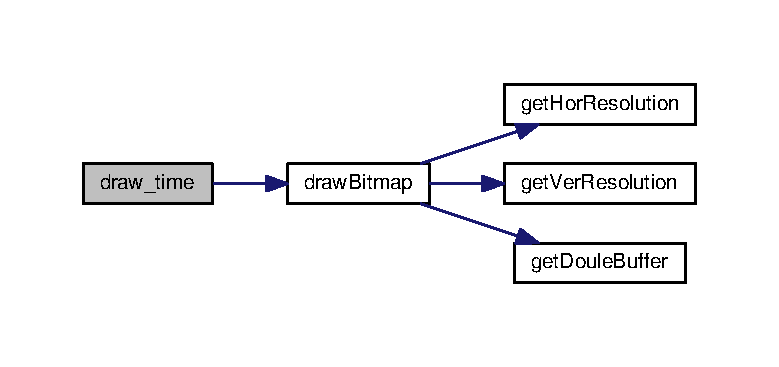
\includegraphics[width=350pt]{group__menu_ga9b565fa7246d14c851c7d66b487e21fc_cgraph}
\end{center}
\end{figure}


\index{menu@{menu}!show\+\_\+points\+\_\+mp@{show\+\_\+points\+\_\+mp}}
\index{show\+\_\+points\+\_\+mp@{show\+\_\+points\+\_\+mp}!menu@{menu}}
\subsubsection[{\texorpdfstring{show\+\_\+points\+\_\+mp(\+Snake $\ast$s1, Snake $\ast$s2)}{show_points_mp(Snake *s1, Snake *s2)}}]{\setlength{\rightskip}{0pt plus 5cm}void show\+\_\+points\+\_\+mp (
\begin{DoxyParamCaption}
\item[{{\bf Snake} $\ast$}]{s1, }
\item[{{\bf Snake} $\ast$}]{s2}
\end{DoxyParamCaption}
)}\hypertarget{group__menu_ga1ceb0e04a7680faf9583052de831fbe6}{}\label{group__menu_ga1ceb0e04a7680faf9583052de831fbe6}


show the end game points of both players snakes (2 snake modes) 


\begin{DoxyParams}{Parameters}
{\em s1} & snake of player 1 points \\
\hline
{\em s2} & snake of player 2 poitns \\
\hline
\end{DoxyParams}


Here is the call graph for this function\+:
\nopagebreak
\begin{figure}[H]
\begin{center}
\leavevmode
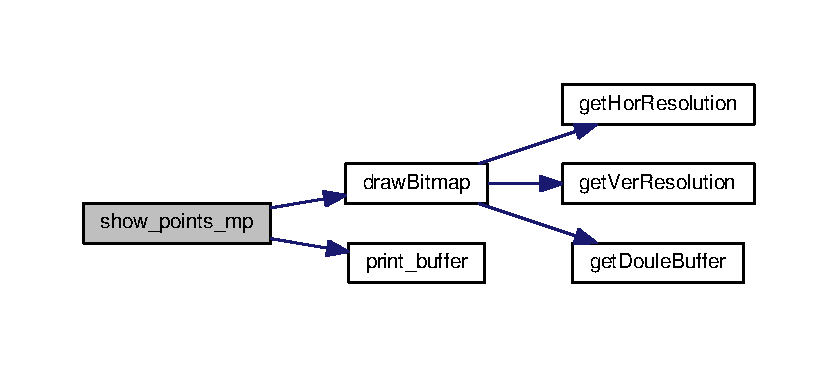
\includegraphics[width=350pt]{group__menu_ga1ceb0e04a7680faf9583052de831fbe6_cgraph}
\end{center}
\end{figure}


\index{menu@{menu}!show\+\_\+points\+\_\+sp@{show\+\_\+points\+\_\+sp}}
\index{show\+\_\+points\+\_\+sp@{show\+\_\+points\+\_\+sp}!menu@{menu}}
\subsubsection[{\texorpdfstring{show\+\_\+points\+\_\+sp(\+Snake $\ast$s1)}{show_points_sp(Snake *s1)}}]{\setlength{\rightskip}{0pt plus 5cm}void show\+\_\+points\+\_\+sp (
\begin{DoxyParamCaption}
\item[{{\bf Snake} $\ast$}]{s1}
\end{DoxyParamCaption}
)}\hypertarget{group__menu_ga2cb72366439253e4818c96e350f195d2}{}\label{group__menu_ga2cb72366439253e4818c96e350f195d2}


show the end game points of the snake(1 snake modes) 


\begin{DoxyParams}{Parameters}
{\em s1} & snake that the points are checked \\
\hline
\end{DoxyParams}


Here is the call graph for this function\+:
\nopagebreak
\begin{figure}[H]
\begin{center}
\leavevmode
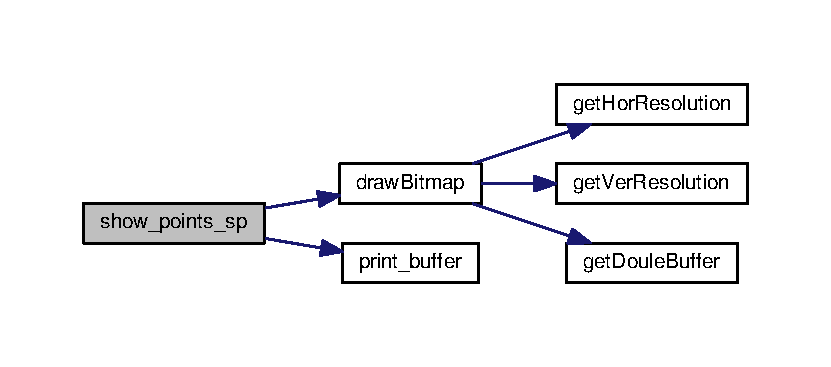
\includegraphics[width=350pt]{group__menu_ga2cb72366439253e4818c96e350f195d2_cgraph}
\end{center}
\end{figure}


\index{menu@{menu}!start\+\_\+variables\+\_\+menu@{start\+\_\+variables\+\_\+menu}}
\index{start\+\_\+variables\+\_\+menu@{start\+\_\+variables\+\_\+menu}!menu@{menu}}
\subsubsection[{\texorpdfstring{start\+\_\+variables\+\_\+menu()}{start_variables_menu()}}]{\setlength{\rightskip}{0pt plus 5cm}void start\+\_\+variables\+\_\+menu (
\begin{DoxyParamCaption}
{}
\end{DoxyParamCaption}
)}\hypertarget{group__menu_gaa00e45cbd295e588746a7f2fd88b0d20}{}\label{group__menu_gaa00e45cbd295e588746a7f2fd88b0d20}


it fills the bmp global variable with the bitmaps loaded in \hyperlink{graphics_8c}{graphics.\+c} 



Here is the call graph for this function\+:
\nopagebreak
\begin{figure}[H]
\begin{center}
\leavevmode
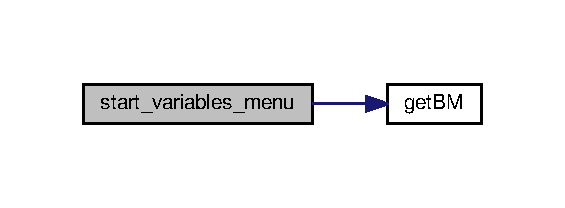
\includegraphics[width=271pt]{group__menu_gaa00e45cbd295e588746a7f2fd88b0d20_cgraph}
\end{center}
\end{figure}


\index{menu@{menu}!update\+\_\+menu\+\_\+mouse@{update\+\_\+menu\+\_\+mouse}}
\index{update\+\_\+menu\+\_\+mouse@{update\+\_\+menu\+\_\+mouse}!menu@{menu}}
\subsubsection[{\texorpdfstring{update\+\_\+menu\+\_\+mouse()}{update_menu_mouse()}}]{\setlength{\rightskip}{0pt plus 5cm}void update\+\_\+menu\+\_\+mouse (
\begin{DoxyParamCaption}
{}
\end{DoxyParamCaption}
)}\hypertarget{group__menu_gab1b3c1e3e90e9c78f31cddcc2544fd09}{}\label{group__menu_gab1b3c1e3e90e9c78f31cddcc2544fd09}


draws in the screen the mouse cursor in the current position of the mouse 



Here is the call graph for this function\+:
\nopagebreak
\begin{figure}[H]
\begin{center}
\leavevmode
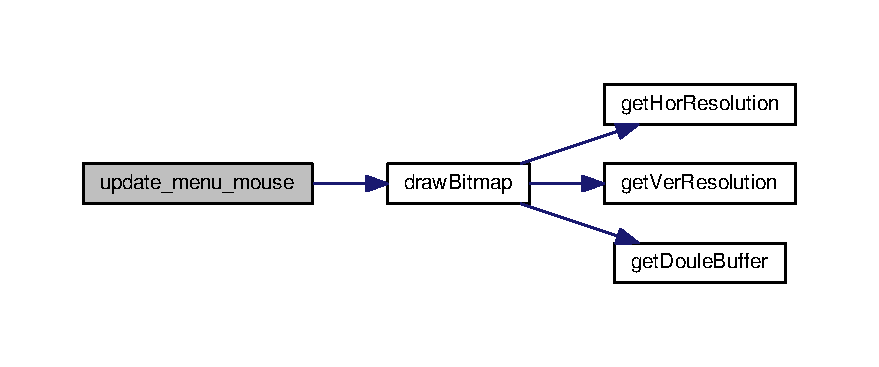
\includegraphics[width=350pt]{group__menu_gab1b3c1e3e90e9c78f31cddcc2544fd09_cgraph}
\end{center}
\end{figure}


\index{menu@{menu}!update\+\_\+pos\+\_\+mouse@{update\+\_\+pos\+\_\+mouse}}
\index{update\+\_\+pos\+\_\+mouse@{update\+\_\+pos\+\_\+mouse}!menu@{menu}}
\subsubsection[{\texorpdfstring{update\+\_\+pos\+\_\+mouse(unsigned long $\ast$x, unsigned long $\ast$y)}{update_pos_mouse(unsigned long *x, unsigned long *y)}}]{\setlength{\rightskip}{0pt plus 5cm}void update\+\_\+pos\+\_\+mouse (
\begin{DoxyParamCaption}
\item[{unsigned long $\ast$}]{x, }
\item[{unsigned long $\ast$}]{y}
\end{DoxyParamCaption}
)}\hypertarget{group__menu_gab149955bb30c6e7a2923c73e86c09ac9}{}\label{group__menu_gab149955bb30c6e7a2923c73e86c09ac9}


it updates the x\+\_\+pos\+\_\+atual and y\+\_\+pos\+\_\+atual of the mouse 


\begin{DoxyParams}{Parameters}
{\em x} & deltax given by the mouse packet(at end x is given the value of the current position of mouse not deltax) \\
\hline
{\em y} & deltay given by the mouse packet(at the end y is given the value of the current position of the mouse not deltay) \\
\hline
\end{DoxyParams}

\hypertarget{group__mouse}{}\section{mouse}
\label{group__mouse}\index{mouse@{mouse}}
\subsection*{Functions}
\begin{DoxyCompactItemize}
\item 
int \hyperlink{group__mouse_ga99506573209b197b84ee22a228b89fbd}{mouse\+\_\+subscribe\+\_\+int} ()
\begin{DoxyCompactList}\small\item\em subscribes and enables the mouse interruts \end{DoxyCompactList}\item 
int \hyperlink{group__mouse_ga685ad2706aca36d9869a30a19b9f446a}{mouse\+\_\+unsubscribe\+\_\+int} ()
\begin{DoxyCompactList}\small\item\em unsubscribes mouse interrupts \end{DoxyCompactList}\item 
unsigned long \hyperlink{group__mouse_ga45c719d8de1147830bd478d4b0e47b97}{mouse\+\_\+int\+\_\+handler} ()
\begin{DoxyCompactList}\small\item\em reads the out bufer of the mouse \end{DoxyCompactList}\item 
int \hyperlink{group__mouse_ga264805a6ca2c11cf80a5e18741400e33}{issue\+\_\+cmd\+\_\+ms} (unsigned long cmd)
\begin{DoxyCompactList}\small\item\em issues a command to the buffer of the mouse \end{DoxyCompactList}\item 
int \hyperlink{group__mouse_ga9bed3f8254b40f5c02cca1cab0551be7}{get\+\_\+packets} (unsigned short $\ast$counter, unsigned long $\ast$packet\+\_\+mouse, unsigned long $\ast$out\+\_\+buf\+\_\+mouse)
\begin{DoxyCompactList}\small\item\em it reads and stores the packet of the mouse \end{DoxyCompactList}\item 
int \hyperlink{group__mouse_gaf578f6a923fae48268dc84dbe1d85c9e}{disable\+\_\+stream\+\_\+mode\+\_\+end} ()
\begin{DoxyCompactList}\small\item\em disables the stream mode of the mouse \end{DoxyCompactList}\item 
int \hyperlink{group__mouse_gabf86ae410ee145ab149b704b7c09d4a0}{set\+\_\+stream\+\_\+mode} ()
\begin{DoxyCompactList}\small\item\em sets and enables the stream mode of the mouse \end{DoxyCompactList}\item 
int \hyperlink{group__mouse_ga04a289fdee2cabf12ec9132bb4ca9add}{print\+\_\+packet} (int size\+\_\+array, unsigned long $\ast$array, long $\ast$x, long $\ast$y, unsigned short $\ast$lb, unsigned short $\ast$rb)
\begin{DoxyCompactList}\small\item\em interprets and prints the contents of a mouse packet,and also store some of its values, like the movement in the x and y axis, the state of both mouse buttons(left and right) \end{DoxyCompactList}\item 
long \hyperlink{group__mouse_ga47845a8af6ede60754da2c4e2540d687}{compl2} (long nr)
\begin{DoxyCompactList}\small\item\em gets a negative number in the complement for 2 mode a returns the absolute value of it \end{DoxyCompactList}\end{DoxyCompactItemize}


\subsection{Detailed Description}
Functions for using the mouse 

\subsection{Function Documentation}
\index{mouse@{mouse}!compl2@{compl2}}
\index{compl2@{compl2}!mouse@{mouse}}
\subsubsection[{\texorpdfstring{compl2(long nr)}{compl2(long nr)}}]{\setlength{\rightskip}{0pt plus 5cm}long compl2 (
\begin{DoxyParamCaption}
\item[{long}]{nr}
\end{DoxyParamCaption}
)}\hypertarget{group__mouse_ga47845a8af6ede60754da2c4e2540d687}{}\label{group__mouse_ga47845a8af6ede60754da2c4e2540d687}


gets a negative number in the complement for 2 mode a returns the absolute value of it 

nr the negative number in compl2 \begin{DoxyReturn}{Returns}
the absolute value 
\end{DoxyReturn}
\index{mouse@{mouse}!disable\+\_\+stream\+\_\+mode\+\_\+end@{disable\+\_\+stream\+\_\+mode\+\_\+end}}
\index{disable\+\_\+stream\+\_\+mode\+\_\+end@{disable\+\_\+stream\+\_\+mode\+\_\+end}!mouse@{mouse}}
\subsubsection[{\texorpdfstring{disable\+\_\+stream\+\_\+mode\+\_\+end()}{disable_stream_mode_end()}}]{\setlength{\rightskip}{0pt plus 5cm}int disable\+\_\+stream\+\_\+mode\+\_\+end (
\begin{DoxyParamCaption}
{}
\end{DoxyParamCaption}
)}\hypertarget{group__mouse_gaf578f6a923fae48268dc84dbe1d85c9e}{}\label{group__mouse_gaf578f6a923fae48268dc84dbe1d85c9e}


disables the stream mode of the mouse 



Here is the call graph for this function\+:
\nopagebreak
\begin{figure}[H]
\begin{center}
\leavevmode
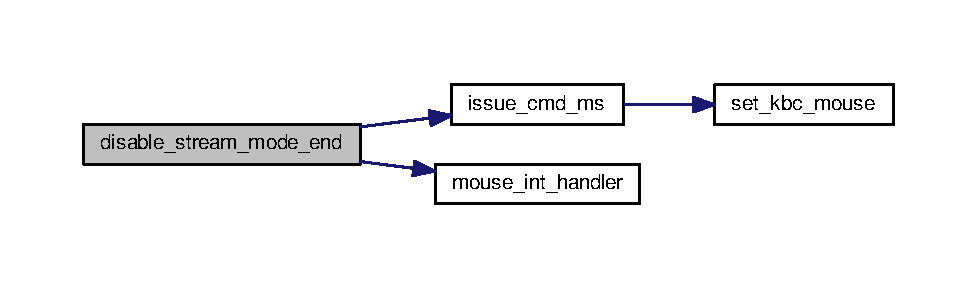
\includegraphics[width=350pt]{group__mouse_gaf578f6a923fae48268dc84dbe1d85c9e_cgraph}
\end{center}
\end{figure}


\index{mouse@{mouse}!get\+\_\+packets@{get\+\_\+packets}}
\index{get\+\_\+packets@{get\+\_\+packets}!mouse@{mouse}}
\subsubsection[{\texorpdfstring{get\+\_\+packets(unsigned short $\ast$counter, unsigned long $\ast$packet\+\_\+mouse, unsigned long $\ast$out\+\_\+buf\+\_\+mouse)}{get_packets(unsigned short *counter, unsigned long *packet_mouse, unsigned long *out_buf_mouse)}}]{\setlength{\rightskip}{0pt plus 5cm}int get\+\_\+packets (
\begin{DoxyParamCaption}
\item[{unsigned short $\ast$}]{counter, }
\item[{unsigned long $\ast$}]{packet\+\_\+mouse, }
\item[{unsigned long $\ast$}]{out\+\_\+buf\+\_\+mouse}
\end{DoxyParamCaption}
)}\hypertarget{group__mouse_ga9bed3f8254b40f5c02cca1cab0551be7}{}\label{group__mouse_ga9bed3f8254b40f5c02cca1cab0551be7}


it reads and stores the packet of the mouse 


\begin{DoxyParams}{Parameters}
{\em counter} & variable to know which element of the packet is being studied (a packet has 3) \\
\hline
{\em packet\+\_\+mouse} & pointer to an array where the packets are stored \\
\hline
{\em out\+\_\+buf\+\_\+mouse} & a content to put on the packet \\
\hline
\end{DoxyParams}
\begin{DoxyReturn}{Returns}
0 if the packet is complete, if packet\+\_\+mouse has been filled, 1 otherwise 
\end{DoxyReturn}


Here is the call graph for this function\+:
\nopagebreak
\begin{figure}[H]
\begin{center}
\leavevmode
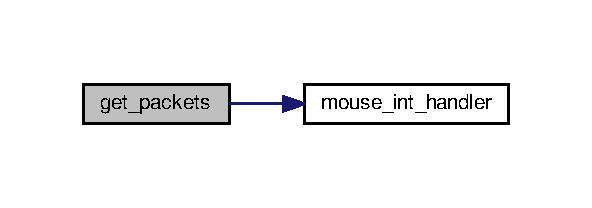
\includegraphics[width=284pt]{group__mouse_ga9bed3f8254b40f5c02cca1cab0551be7_cgraph}
\end{center}
\end{figure}


\index{mouse@{mouse}!issue\+\_\+cmd\+\_\+ms@{issue\+\_\+cmd\+\_\+ms}}
\index{issue\+\_\+cmd\+\_\+ms@{issue\+\_\+cmd\+\_\+ms}!mouse@{mouse}}
\subsubsection[{\texorpdfstring{issue\+\_\+cmd\+\_\+ms(unsigned long cmd)}{issue_cmd_ms(unsigned long cmd)}}]{\setlength{\rightskip}{0pt plus 5cm}int issue\+\_\+cmd\+\_\+ms (
\begin{DoxyParamCaption}
\item[{unsigned long}]{cmd}
\end{DoxyParamCaption}
)}\hypertarget{group__mouse_ga264805a6ca2c11cf80a5e18741400e33}{}\label{group__mouse_ga264805a6ca2c11cf80a5e18741400e33}


issues a command to the buffer of the mouse 


\begin{DoxyParams}{Parameters}
{\em cmd} & command or arguments issued \\
\hline
\end{DoxyParams}
\begin{DoxyReturn}{Returns}
0 if succeeds 1 otherwise 
\end{DoxyReturn}


Here is the call graph for this function\+:
\nopagebreak
\begin{figure}[H]
\begin{center}
\leavevmode
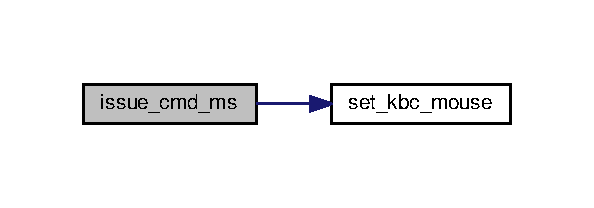
\includegraphics[width=285pt]{group__mouse_ga264805a6ca2c11cf80a5e18741400e33_cgraph}
\end{center}
\end{figure}


\index{mouse@{mouse}!mouse\+\_\+int\+\_\+handler@{mouse\+\_\+int\+\_\+handler}}
\index{mouse\+\_\+int\+\_\+handler@{mouse\+\_\+int\+\_\+handler}!mouse@{mouse}}
\subsubsection[{\texorpdfstring{mouse\+\_\+int\+\_\+handler()}{mouse_int_handler()}}]{\setlength{\rightskip}{0pt plus 5cm}unsigned long mouse\+\_\+int\+\_\+handler (
\begin{DoxyParamCaption}
{}
\end{DoxyParamCaption}
)}\hypertarget{group__mouse_ga45c719d8de1147830bd478d4b0e47b97}{}\label{group__mouse_ga45c719d8de1147830bd478d4b0e47b97}


reads the out bufer of the mouse 

\begin{DoxyReturn}{Returns}
the value of the buffer or -\/1 if it failed 
\end{DoxyReturn}
\index{mouse@{mouse}!mouse\+\_\+subscribe\+\_\+int@{mouse\+\_\+subscribe\+\_\+int}}
\index{mouse\+\_\+subscribe\+\_\+int@{mouse\+\_\+subscribe\+\_\+int}!mouse@{mouse}}
\subsubsection[{\texorpdfstring{mouse\+\_\+subscribe\+\_\+int()}{mouse_subscribe_int()}}]{\setlength{\rightskip}{0pt plus 5cm}int mouse\+\_\+subscribe\+\_\+int (
\begin{DoxyParamCaption}
{}
\end{DoxyParamCaption}
)}\hypertarget{group__mouse_ga99506573209b197b84ee22a228b89fbd}{}\label{group__mouse_ga99506573209b197b84ee22a228b89fbd}


subscribes and enables the mouse interruts 

\begin{DoxyReturn}{Returns}
the changed hook\+\_\+id or -\/1 if it failed 
\end{DoxyReturn}
\index{mouse@{mouse}!mouse\+\_\+unsubscribe\+\_\+int@{mouse\+\_\+unsubscribe\+\_\+int}}
\index{mouse\+\_\+unsubscribe\+\_\+int@{mouse\+\_\+unsubscribe\+\_\+int}!mouse@{mouse}}
\subsubsection[{\texorpdfstring{mouse\+\_\+unsubscribe\+\_\+int()}{mouse_unsubscribe_int()}}]{\setlength{\rightskip}{0pt plus 5cm}int mouse\+\_\+unsubscribe\+\_\+int (
\begin{DoxyParamCaption}
{}
\end{DoxyParamCaption}
)}\hypertarget{group__mouse_ga685ad2706aca36d9869a30a19b9f446a}{}\label{group__mouse_ga685ad2706aca36d9869a30a19b9f446a}


unsubscribes mouse interrupts 

\begin{DoxyReturn}{Returns}
1 if it failed,0 otherwise 
\end{DoxyReturn}
\index{mouse@{mouse}!print\+\_\+packet@{print\+\_\+packet}}
\index{print\+\_\+packet@{print\+\_\+packet}!mouse@{mouse}}
\subsubsection[{\texorpdfstring{print\+\_\+packet(int size\+\_\+array, unsigned long $\ast$array, long $\ast$x, long $\ast$y, unsigned short $\ast$lb, unsigned short $\ast$rb)}{print_packet(int size_array, unsigned long *array, long *x, long *y, unsigned short *lb, unsigned short *rb)}}]{\setlength{\rightskip}{0pt plus 5cm}int print\+\_\+packet (
\begin{DoxyParamCaption}
\item[{int}]{size\+\_\+array, }
\item[{unsigned long $\ast$}]{array, }
\item[{long $\ast$}]{x, }
\item[{long $\ast$}]{y, }
\item[{unsigned short $\ast$}]{lb, }
\item[{unsigned short $\ast$}]{rb}
\end{DoxyParamCaption}
)}\hypertarget{group__mouse_ga04a289fdee2cabf12ec9132bb4ca9add}{}\label{group__mouse_ga04a289fdee2cabf12ec9132bb4ca9add}


interprets and prints the contents of a mouse packet,and also store some of its values, like the movement in the x and y axis, the state of both mouse buttons(left and right) 


\begin{DoxyParams}{Parameters}
{\em size\+\_\+array} & the size of the array packet (is always 3 ) \\
\hline
{\em array} & pointer to the first element of the packet array \\
\hline
{\em x} & variable where is going to be stored the movement in the x axis of the mouse \\
\hline
{\em y} & variable where is going to be stored the movement in the y axis of the mouse \\
\hline
{\em lb} & variable where the state of the left mouse button is saved \\
\hline
{\em rb} & variable where the state of the right mouse button is saved \\
\hline
\end{DoxyParams}
\begin{DoxyReturn}{Returns}
1 overflow is verified in any of the axiss 
\end{DoxyReturn}


Here is the call graph for this function\+:
\nopagebreak
\begin{figure}[H]
\begin{center}
\leavevmode
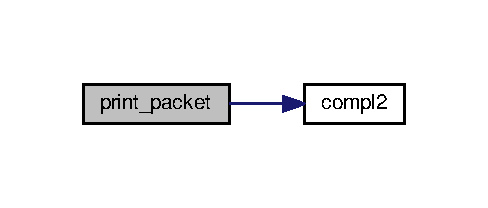
\includegraphics[width=234pt]{group__mouse_ga04a289fdee2cabf12ec9132bb4ca9add_cgraph}
\end{center}
\end{figure}


\index{mouse@{mouse}!set\+\_\+stream\+\_\+mode@{set\+\_\+stream\+\_\+mode}}
\index{set\+\_\+stream\+\_\+mode@{set\+\_\+stream\+\_\+mode}!mouse@{mouse}}
\subsubsection[{\texorpdfstring{set\+\_\+stream\+\_\+mode()}{set_stream_mode()}}]{\setlength{\rightskip}{0pt plus 5cm}int set\+\_\+stream\+\_\+mode (
\begin{DoxyParamCaption}
{}
\end{DoxyParamCaption}
)}\hypertarget{group__mouse_gabf86ae410ee145ab149b704b7c09d4a0}{}\label{group__mouse_gabf86ae410ee145ab149b704b7c09d4a0}


sets and enables the stream mode of the mouse 



Here is the call graph for this function\+:
\nopagebreak
\begin{figure}[H]
\begin{center}
\leavevmode
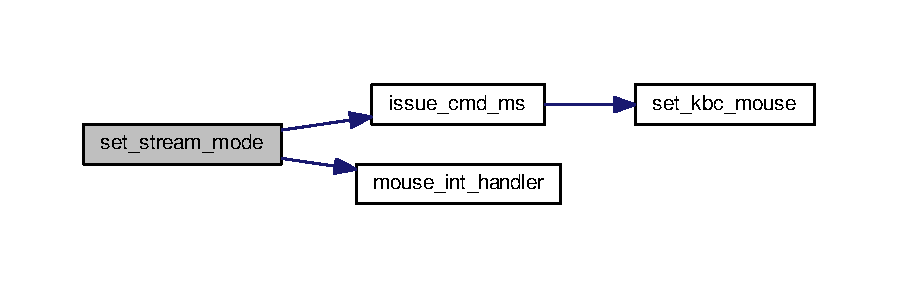
\includegraphics[width=350pt]{group__mouse_gabf86ae410ee145ab149b704b7c09d4a0_cgraph}
\end{center}
\end{figure}



\hypertarget{group__object}{}\section{object}
\label{group__object}\index{object@{object}}
\subsection*{Classes}
\begin{DoxyCompactItemize}
\item 
struct \hyperlink{structGame__object}{Game\+\_\+object}
\end{DoxyCompactItemize}
\subsection*{Functions}
\begin{DoxyCompactItemize}
\item 
void \hyperlink{group__object_gaec22a837ae65e3ba7f3e55ad9c37c91d}{new\+\_\+object} (\hyperlink{structGame__object}{Game\+\_\+object} $\ast$obj, \hyperlink{group__object_ga90ab20efa1890ce46e743d7569ce7cec}{object\+\_\+name} name)
\begin{DoxyCompactList}\small\item\em it creates a new object in a random position \end{DoxyCompactList}\end{DoxyCompactItemize}
\subsection*{Variables}
\begin{DoxyCompactItemize}
\item 
unsigned short \hyperlink{group__object_ga41a0b70059db5a8364cb00caed5f7860}{Game\+\_\+object\+::row}
\item 
unsigned short \hyperlink{group__object_ga26747c58af9aac0a386f3be5b5302d23}{Game\+\_\+object\+::col}
\begin{DoxyCompactList}\small\item\em position in the matrix\+\_\+graphics \end{DoxyCompactList}\item 
int \hyperlink{group__object_gaa3e8af9c364161ddf47359bba651e9cf}{Game\+\_\+object\+::point\+\_\+value}
\item 
\hyperlink{group__object_ga90ab20efa1890ce46e743d7569ce7cec}{object\+\_\+name} \hyperlink{group__object_ga27d8ddc2e36ab28af25f9698f1b11e49}{Game\+\_\+object\+::name}
\begin{DoxyCompactList}\small\item\em how many points the object is valued (U\+N\+U\+S\+ED) \end{DoxyCompactList}\end{DoxyCompactItemize}
\subsection*{object\+\_\+name}
\begin{DoxyCompactItemize}
\item 
enum \hyperlink{group__object_ga90ab20efa1890ce46e743d7569ce7cec}{object\+\_\+name} \{ \hyperlink{group__object_gga90ab20efa1890ce46e743d7569ce7ceca61dca5db46c7857556e7eaced30c879b}{F\+R\+U\+IT}, 
\hyperlink{group__object_gga90ab20efa1890ce46e743d7569ce7ceca095285ba8fb2e1f9cfb29c80546f06e4}{B\+O\+MB}
 \}
\end{DoxyCompactItemize}


\subsection{Detailed Description}
Creation of an object 

\subsection{Enumeration Type Documentation}
\index{object@{object}!object\+\_\+name@{object\+\_\+name}}
\index{object\+\_\+name@{object\+\_\+name}!object@{object}}
\subsubsection[{\texorpdfstring{object\+\_\+name}{object_name}}]{\setlength{\rightskip}{0pt plus 5cm}enum {\bf object\+\_\+name}}\hypertarget{group__object_ga90ab20efa1890ce46e743d7569ce7cec}{}\label{group__object_ga90ab20efa1890ce46e743d7569ce7cec}
Name associations to a specific object \begin{Desc}
\item[Enumerator]\par
\begin{description}
\index{F\+R\+U\+IT@{F\+R\+U\+IT}!object@{object}}\index{object@{object}!F\+R\+U\+IT@{F\+R\+U\+IT}}\item[{\em 
F\+R\+U\+IT\hypertarget{group__object_gga90ab20efa1890ce46e743d7569ce7ceca61dca5db46c7857556e7eaced30c879b}{}\label{group__object_gga90ab20efa1890ce46e743d7569ce7ceca61dca5db46c7857556e7eaced30c879b}
}]\index{B\+O\+MB@{B\+O\+MB}!object@{object}}\index{object@{object}!B\+O\+MB@{B\+O\+MB}}\item[{\em 
B\+O\+MB\hypertarget{group__object_gga90ab20efa1890ce46e743d7569ce7ceca095285ba8fb2e1f9cfb29c80546f06e4}{}\label{group__object_gga90ab20efa1890ce46e743d7569ce7ceca095285ba8fb2e1f9cfb29c80546f06e4}
}]\end{description}
\end{Desc}


\subsection{Function Documentation}
\index{object@{object}!new\+\_\+object@{new\+\_\+object}}
\index{new\+\_\+object@{new\+\_\+object}!object@{object}}
\subsubsection[{\texorpdfstring{new\+\_\+object(\+Game\+\_\+object $\ast$obj, object\+\_\+name name)}{new_object(Game_object *obj, object_name name)}}]{\setlength{\rightskip}{0pt plus 5cm}void new\+\_\+object (
\begin{DoxyParamCaption}
\item[{{\bf Game\+\_\+object} $\ast$}]{obj, }
\item[{{\bf object\+\_\+name}}]{name}
\end{DoxyParamCaption}
)}\hypertarget{group__object_gaec22a837ae65e3ba7f3e55ad9c37c91d}{}\label{group__object_gaec22a837ae65e3ba7f3e55ad9c37c91d}


it creates a new object in a random position 


\begin{DoxyParams}{Parameters}
{\em obj} & object that is going to be built \\
\hline
{\em name} & name of the object to know what type it is \\
\hline
\end{DoxyParams}


\subsection{Variable Documentation}
\index{object@{object}!col@{col}}
\index{col@{col}!object@{object}}
\subsubsection[{\texorpdfstring{col}{col}}]{\setlength{\rightskip}{0pt plus 5cm}unsigned short Game\+\_\+object\+::col}\hypertarget{group__object_ga26747c58af9aac0a386f3be5b5302d23}{}\label{group__object_ga26747c58af9aac0a386f3be5b5302d23}


position in the matrix\+\_\+graphics 

\index{object@{object}!name@{name}}
\index{name@{name}!object@{object}}
\subsubsection[{\texorpdfstring{name}{name}}]{\setlength{\rightskip}{0pt plus 5cm}{\bf object\+\_\+name} Game\+\_\+object\+::name}\hypertarget{group__object_ga27d8ddc2e36ab28af25f9698f1b11e49}{}\label{group__object_ga27d8ddc2e36ab28af25f9698f1b11e49}


how many points the object is valued (U\+N\+U\+S\+ED) 

$<$name of the object of type object\+\_\+name \index{object@{object}!point\+\_\+value@{point\+\_\+value}}
\index{point\+\_\+value@{point\+\_\+value}!object@{object}}
\subsubsection[{\texorpdfstring{point\+\_\+value}{point_value}}]{\setlength{\rightskip}{0pt plus 5cm}int Game\+\_\+object\+::point\+\_\+value}\hypertarget{group__object_gaa3e8af9c364161ddf47359bba651e9cf}{}\label{group__object_gaa3e8af9c364161ddf47359bba651e9cf}
\index{object@{object}!row@{row}}
\index{row@{row}!object@{object}}
\subsubsection[{\texorpdfstring{row}{row}}]{\setlength{\rightskip}{0pt plus 5cm}unsigned short Game\+\_\+object\+::row}\hypertarget{group__object_ga41a0b70059db5a8364cb00caed5f7860}{}\label{group__object_ga41a0b70059db5a8364cb00caed5f7860}

\hypertarget{group__rtc}{}\section{rtc}
\label{group__rtc}\index{rtc@{rtc}}
\subsection*{Functions}
\begin{DoxyCompactItemize}
\item 
int \hyperlink{group__rtc_ga5960e020c86a383a63cdead42f3928b9}{can\+\_\+read\+\_\+date} ()
\begin{DoxyCompactList}\small\item\em simple function that sees if the date can be read \end{DoxyCompactList}\item 
int \hyperlink{group__rtc_gae1b1b1cc88f89eae300cdeef578da474}{is\+\_\+binary} ()
\begin{DoxyCompactList}\small\item\em verify if real time clock is on binary mode \end{DoxyCompactList}\item 
int \hyperlink{group__rtc_ga841ea89e213413164d1e5e4a9394a955}{bcd\+\_\+to\+\_\+decimal} (unsigned long number)
\begin{DoxyCompactList}\small\item\em it \char`\"{}transforms\char`\"{} a binary number to a decimal one \end{DoxyCompactList}\item 
void \hyperlink{group__rtc_ga2ed53b5a2ef633341d444c26659c2e58}{read\+\_\+date} (unsigned long $\ast$day, unsigned long $\ast$month, unsigned long $\ast$year)
\begin{DoxyCompactList}\small\item\em reads the right registers of the rtc to get the date of the system \end{DoxyCompactList}\item 
void \hyperlink{group__rtc_ga361f06856ed8c5dfb47c2e01af6a7470}{read\+\_\+time} (unsigned long $\ast$hour, unsigned long $\ast$minute, unsigned long $\ast$sec)
\begin{DoxyCompactList}\small\item\em reads the necessary registers of the rtc to get the time of the system \end{DoxyCompactList}\end{DoxyCompactItemize}


\subsection{Detailed Description}
Functions related to the rtc 

\subsection{Function Documentation}
\index{rtc@{rtc}!bcd\+\_\+to\+\_\+decimal@{bcd\+\_\+to\+\_\+decimal}}
\index{bcd\+\_\+to\+\_\+decimal@{bcd\+\_\+to\+\_\+decimal}!rtc@{rtc}}
\subsubsection[{\texorpdfstring{bcd\+\_\+to\+\_\+decimal(unsigned long number)}{bcd_to_decimal(unsigned long number)}}]{\setlength{\rightskip}{0pt plus 5cm}int bcd\+\_\+to\+\_\+decimal (
\begin{DoxyParamCaption}
\item[{unsigned long}]{number}
\end{DoxyParamCaption}
)}\hypertarget{group__rtc_ga841ea89e213413164d1e5e4a9394a955}{}\label{group__rtc_ga841ea89e213413164d1e5e4a9394a955}


it \char`\"{}transforms\char`\"{} a binary number to a decimal one 


\begin{DoxyParams}{Parameters}
{\em number} & in binary that is going to change to decimal \\
\hline
\end{DoxyParams}
\begin{DoxyReturn}{Returns}
the decimal number got 
\end{DoxyReturn}
\index{rtc@{rtc}!can\+\_\+read\+\_\+date@{can\+\_\+read\+\_\+date}}
\index{can\+\_\+read\+\_\+date@{can\+\_\+read\+\_\+date}!rtc@{rtc}}
\subsubsection[{\texorpdfstring{can\+\_\+read\+\_\+date()}{can_read_date()}}]{\setlength{\rightskip}{0pt plus 5cm}int can\+\_\+read\+\_\+date (
\begin{DoxyParamCaption}
{}
\end{DoxyParamCaption}
)}\hypertarget{group__rtc_ga5960e020c86a383a63cdead42f3928b9}{}\label{group__rtc_ga5960e020c86a383a63cdead42f3928b9}


simple function that sees if the date can be read 

\begin{DoxyReturn}{Returns}
1 if it cannot be read 0 otherwise 
\end{DoxyReturn}
\index{rtc@{rtc}!is\+\_\+binary@{is\+\_\+binary}}
\index{is\+\_\+binary@{is\+\_\+binary}!rtc@{rtc}}
\subsubsection[{\texorpdfstring{is\+\_\+binary()}{is_binary()}}]{\setlength{\rightskip}{0pt plus 5cm}int is\+\_\+binary (
\begin{DoxyParamCaption}
{}
\end{DoxyParamCaption}
)}\hypertarget{group__rtc_gae1b1b1cc88f89eae300cdeef578da474}{}\label{group__rtc_gae1b1b1cc88f89eae300cdeef578da474}


verify if real time clock is on binary mode 

\begin{DoxyReturn}{Returns}
return 1 if is on bcd mode and 0 if is on binary mode 
\end{DoxyReturn}
\index{rtc@{rtc}!read\+\_\+date@{read\+\_\+date}}
\index{read\+\_\+date@{read\+\_\+date}!rtc@{rtc}}
\subsubsection[{\texorpdfstring{read\+\_\+date(unsigned long $\ast$day, unsigned long $\ast$month, unsigned long $\ast$year)}{read_date(unsigned long *day, unsigned long *month, unsigned long *year)}}]{\setlength{\rightskip}{0pt plus 5cm}void read\+\_\+date (
\begin{DoxyParamCaption}
\item[{unsigned long $\ast$}]{day, }
\item[{unsigned long $\ast$}]{month, }
\item[{unsigned long $\ast$}]{year}
\end{DoxyParamCaption}
)}\hypertarget{group__rtc_ga2ed53b5a2ef633341d444c26659c2e58}{}\label{group__rtc_ga2ed53b5a2ef633341d444c26659c2e58}


reads the right registers of the rtc to get the date of the system 


\begin{DoxyParams}{Parameters}
{\em day} & variable where the day read is going to be stored \\
\hline
{\em month} & variable where the month read is going to be stored \\
\hline
{\em year} & variable where the year read is going to be stored \\
\hline
\end{DoxyParams}
\index{rtc@{rtc}!read\+\_\+time@{read\+\_\+time}}
\index{read\+\_\+time@{read\+\_\+time}!rtc@{rtc}}
\subsubsection[{\texorpdfstring{read\+\_\+time(unsigned long $\ast$hour, unsigned long $\ast$minute, unsigned long $\ast$sec)}{read_time(unsigned long *hour, unsigned long *minute, unsigned long *sec)}}]{\setlength{\rightskip}{0pt plus 5cm}void read\+\_\+time (
\begin{DoxyParamCaption}
\item[{unsigned long $\ast$}]{hour, }
\item[{unsigned long $\ast$}]{minute, }
\item[{unsigned long $\ast$}]{sec}
\end{DoxyParamCaption}
)}\hypertarget{group__rtc_ga361f06856ed8c5dfb47c2e01af6a7470}{}\label{group__rtc_ga361f06856ed8c5dfb47c2e01af6a7470}


reads the necessary registers of the rtc to get the time of the system 


\begin{DoxyParams}{Parameters}
{\em hour} & variable where the hour is going to be stored \\
\hline
{\em minute} & variable where the minutes are going to be stored \\
\hline
{\em sec} & variable where the seconds are going to be stored \\
\hline
\end{DoxyParams}

\hypertarget{group__snake}{}\section{snake}
\label{group__snake}\index{snake@{snake}}
\subsection*{Classes}
\begin{DoxyCompactItemize}
\item 
struct \hyperlink{structSegment}{Segment}
\item 
struct \hyperlink{structSnake}{Snake}
\begin{DoxyCompactList}\small\item\em Represents a \hyperlink{structSnake}{Snake}. \end{DoxyCompactList}\end{DoxyCompactItemize}
\subsection*{Functions}
\begin{DoxyCompactItemize}
\item 
void \hyperlink{group__snake_ga9905deea86c0d94567ede79df04a2917}{add\+\_\+segment} (\hyperlink{structSnake}{Snake} $\ast$\hyperlink{group__man__events_gaf79c0d77b0cca9ebf96bbbed1f88aed0}{s1}, unsigned short row, unsigned short col)
\begin{DoxyCompactList}\small\item\em adds a new segment\+\_\+snake to the snake as the new head of the snake \end{DoxyCompactList}\item 
void \hyperlink{group__snake_ga0da33cffbcc02a3da21cb4b74271c429}{new\+\_\+snake} (int size, unsigned short x, unsigned short y, \hyperlink{structSnake}{Snake} $\ast$\hyperlink{group__man__events_gaf79c0d77b0cca9ebf96bbbed1f88aed0}{s1})
\begin{DoxyCompactList}\small\item\em creates a new snake \end{DoxyCompactList}\item 
void \hyperlink{group__snake_ga0ff179758d3dbd6aa7c79dc51776c9d7}{move\+\_\+snake} (\hyperlink{structSnake}{Snake} $\ast$\hyperlink{group__man__events_gaf79c0d77b0cca9ebf96bbbed1f88aed0}{s1})
\begin{DoxyCompactList}\small\item\em moves the snake by one position based on its segments direction and orientation \end{DoxyCompactList}\item 
void \hyperlink{group__snake_gabc6924be4961d75d44ed29f0a4ed5bbb}{set\+\_\+boost} (\hyperlink{structSnake}{Snake} $\ast$\hyperlink{group__man__events_gaf79c0d77b0cca9ebf96bbbed1f88aed0}{s1})
\begin{DoxyCompactList}\small\item\em sets the boost flag and doubles the snake velocity \end{DoxyCompactList}\item 
void \hyperlink{group__snake_ga471508bb9844c474f3c27e078aecc638}{stop\+\_\+boost} (\hyperlink{structSnake}{Snake} $\ast$\hyperlink{group__man__events_gaf79c0d77b0cca9ebf96bbbed1f88aed0}{s1})
\begin{DoxyCompactList}\small\item\em resets the boost flag and decreases the snake velocity \end{DoxyCompactList}\item 
void \hyperlink{group__snake_gafc851c81ca29b4d1e7e8890e7bf6bbf0}{set\+\_\+snake} (\hyperlink{structSnake}{Snake} $\ast$snake, int col)
\begin{DoxyCompactList}\small\item\em resets the snake that is used in the menu preview(when choosing the snake skin) \end{DoxyCompactList}\item 
void \hyperlink{group__snake_ga155db98fd681adcf82c1d07b8c4372f8}{inc\+\_\+snake} (\hyperlink{structSnake}{Snake} $\ast$\hyperlink{group__man__events_gaf79c0d77b0cca9ebf96bbbed1f88aed0}{s1})
\begin{DoxyCompactList}\small\item\em increases the size of the snake by adding a new segment as the tail of the snake \end{DoxyCompactList}\end{DoxyCompactItemize}
\subsection*{Variables}
\begin{DoxyCompactItemize}
\item 
unsigned short \hyperlink{group__snake_ga5c86edfec316ae4d5033a85525babed6}{Segment\+::row}
\item 
unsigned short \hyperlink{group__snake_ga3369387554e0ec37bb04c153c3529ed9}{Segment\+::col}
\begin{DoxyCompactList}\small\item\em position in the matrix\+\_\+graphics \end{DoxyCompactList}\item 
unsigned short \hyperlink{group__snake_gacf610091b7f59fb0f1f37c6df4e14c18}{Segment\+::direction}
\begin{DoxyCompactList}\small\item\em direction it is facing, vertical or horizontal \end{DoxyCompactList}\item 
unsigned short \hyperlink{group__snake_gadd6c62d3fd2c3aab9175c07694fdc075}{Segment\+::orientation}
\item 
struct \hyperlink{structSegment}{Segment} $\ast$ \hyperlink{group__snake_ga20fb1741f720a656ec35972c2305a2d9}{Segment\+::next}
\begin{DoxyCompactList}\small\item\em orientation it is facing. if its moving in positive direction or negative \end{DoxyCompactList}\item 
struct \hyperlink{structSegment}{Segment} $\ast$ \hyperlink{group__snake_ga60c4d032ff0baffc3c99c1630dae24e3}{Segment\+::before}
\begin{DoxyCompactList}\small\item\em pointer to the next body part(like a linked list) \end{DoxyCompactList}\item 
\hyperlink{group__snake_ga40f634d31a1f9372bd182d65da207a21}{segment\+\_\+snake} $\ast$ \hyperlink{group__snake_gaf63e50ac65f365d67ae3975a178cba8c}{Snake\+::head}
\begin{DoxyCompactList}\small\item\em pointer to the head of the snake \end{DoxyCompactList}\item 
\hyperlink{group__snake_ga40f634d31a1f9372bd182d65da207a21}{segment\+\_\+snake} $\ast$ \hyperlink{group__snake_gada92e10f60af5b1afdb7318df07a1a33}{Snake\+::tail}
\item 
unsigned int \hyperlink{group__snake_ga29ba822024f7651a9fa0c80df840252b}{Snake\+::size}
\begin{DoxyCompactList}\small\item\em pointer to the tail of the snake \end{DoxyCompactList}\item 
unsigned short \hyperlink{group__snake_gac444a5a9306233f5be0b603335785b3d}{Snake\+::velocity}
\begin{DoxyCompactList}\small\item\em size of the snake(number of segment\+\_\+snake) \end{DoxyCompactList}\item 
unsigned short \hyperlink{group__snake_ga7339bbc2027ffeb1ce00f24a834610cc}{Snake\+::boost}
\begin{DoxyCompactList}\small\item\em velocity the snake is moving \end{DoxyCompactList}\item 
unsigned short \hyperlink{group__snake_ga0b46bc6b402fd8999c6998eca1806c3e}{Snake\+::boost\+\_\+time}
\begin{DoxyCompactList}\small\item\em flag to know if the snake is boosting \end{DoxyCompactList}\end{DoxyCompactItemize}
\subsection*{Snake}
\begin{DoxyCompactItemize}
\item 
typedef struct \hyperlink{structSegment}{Segment} \hyperlink{group__snake_ga40f634d31a1f9372bd182d65da207a21}{segment\+\_\+snake}
\end{DoxyCompactItemize}


\subsection{Detailed Description}
Functions associated with the creation of the snake and its movements 

\subsection{Typedef Documentation}
\index{snake@{snake}!segment\+\_\+snake@{segment\+\_\+snake}}
\index{segment\+\_\+snake@{segment\+\_\+snake}!snake@{snake}}
\subsubsection[{\texorpdfstring{segment\+\_\+snake}{segment_snake}}]{\setlength{\rightskip}{0pt plus 5cm}typedef struct {\bf Segment} {\bf segment\+\_\+snake}}\hypertarget{group__snake_ga40f634d31a1f9372bd182d65da207a21}{}\label{group__snake_ga40f634d31a1f9372bd182d65da207a21}
\hyperlink{structSnake}{Snake} using a linked list 

\subsection{Function Documentation}
\index{snake@{snake}!add\+\_\+segment@{add\+\_\+segment}}
\index{add\+\_\+segment@{add\+\_\+segment}!snake@{snake}}
\subsubsection[{\texorpdfstring{add\+\_\+segment(\+Snake $\ast$s1, unsigned short row, unsigned short col)}{add_segment(Snake *s1, unsigned short row, unsigned short col)}}]{\setlength{\rightskip}{0pt plus 5cm}void add\+\_\+segment (
\begin{DoxyParamCaption}
\item[{{\bf Snake} $\ast$}]{s1, }
\item[{unsigned short}]{row, }
\item[{unsigned short}]{col}
\end{DoxyParamCaption}
)}\hypertarget{group__snake_ga9905deea86c0d94567ede79df04a2917}{}\label{group__snake_ga9905deea86c0d94567ede79df04a2917}


adds a new segment\+\_\+snake to the snake as the new head of the snake 


\begin{DoxyParams}{Parameters}
{\em s1} & snake which the new segment is going to be added \\
\hline
{\em row} & member row of the new segment \\
\hline
{\em col} & member col of the new segment\\
\hline
\end{DoxyParams}
The last elements of the new segment, are based on the segments of the snake(especially the head) \index{snake@{snake}!inc\+\_\+snake@{inc\+\_\+snake}}
\index{inc\+\_\+snake@{inc\+\_\+snake}!snake@{snake}}
\subsubsection[{\texorpdfstring{inc\+\_\+snake(\+Snake $\ast$s1)}{inc_snake(Snake *s1)}}]{\setlength{\rightskip}{0pt plus 5cm}void inc\+\_\+snake (
\begin{DoxyParamCaption}
\item[{{\bf Snake} $\ast$}]{s1}
\end{DoxyParamCaption}
)}\hypertarget{group__snake_ga155db98fd681adcf82c1d07b8c4372f8}{}\label{group__snake_ga155db98fd681adcf82c1d07b8c4372f8}


increases the size of the snake by adding a new segment as the tail of the snake 


\begin{DoxyParams}{Parameters}
{\em s1} & snake which is going to increase\\
\hline
\end{DoxyParams}
It is used when the snake eats a fruit, it is basically add\+\_\+segment but a little more restrictive \index{snake@{snake}!move\+\_\+snake@{move\+\_\+snake}}
\index{move\+\_\+snake@{move\+\_\+snake}!snake@{snake}}
\subsubsection[{\texorpdfstring{move\+\_\+snake(\+Snake $\ast$s1)}{move_snake(Snake *s1)}}]{\setlength{\rightskip}{0pt plus 5cm}void move\+\_\+snake (
\begin{DoxyParamCaption}
\item[{{\bf Snake} $\ast$}]{s1}
\end{DoxyParamCaption}
)}\hypertarget{group__snake_ga0ff179758d3dbd6aa7c79dc51776c9d7}{}\label{group__snake_ga0ff179758d3dbd6aa7c79dc51776c9d7}


moves the snake by one position based on its segments direction and orientation 


\begin{DoxyParams}{Parameters}
{\em s1} & snake that is going to be moved\\
\hline
\end{DoxyParams}
Basically it moves by just removing the tail of the snake and create and put a new head 

Here is the call graph for this function\+:
\nopagebreak
\begin{figure}[H]
\begin{center}
\leavevmode
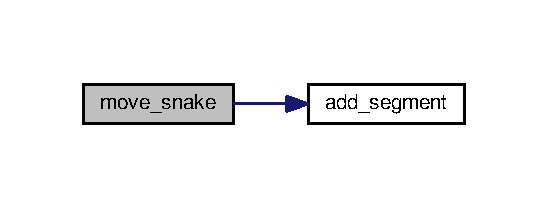
\includegraphics[width=263pt]{group__snake_ga0ff179758d3dbd6aa7c79dc51776c9d7_cgraph}
\end{center}
\end{figure}


\index{snake@{snake}!new\+\_\+snake@{new\+\_\+snake}}
\index{new\+\_\+snake@{new\+\_\+snake}!snake@{snake}}
\subsubsection[{\texorpdfstring{new\+\_\+snake(int size, unsigned short x, unsigned short y, Snake $\ast$s1)}{new_snake(int size, unsigned short x, unsigned short y, Snake *s1)}}]{\setlength{\rightskip}{0pt plus 5cm}void new\+\_\+snake (
\begin{DoxyParamCaption}
\item[{int}]{size, }
\item[{unsigned short}]{x, }
\item[{unsigned short}]{y, }
\item[{{\bf Snake} $\ast$}]{s1}
\end{DoxyParamCaption}
)}\hypertarget{group__snake_ga0da33cffbcc02a3da21cb4b74271c429}{}\label{group__snake_ga0da33cffbcc02a3da21cb4b74271c429}


creates a new snake 


\begin{DoxyParams}{Parameters}
{\em size} & number of segments the snake is going to have(add\+\_\+segment is used for this) \\
\hline
{\em x} & the row member of all segments of the new snake \\
\hline
{\em y} & the col member of all segments of the new snake \\
\hline
{\em s1} & the variable where the snake is going to be saved Every new snake and its segments have the direction(horizontal) and oriectation(positive) as default \\
\hline
\end{DoxyParams}


Here is the call graph for this function\+:
\nopagebreak
\begin{figure}[H]
\begin{center}
\leavevmode
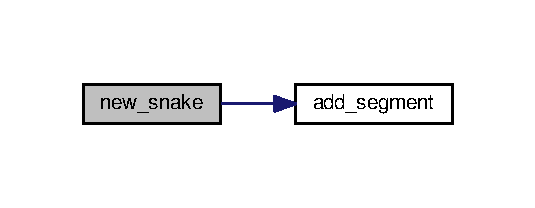
\includegraphics[width=257pt]{group__snake_ga0da33cffbcc02a3da21cb4b74271c429_cgraph}
\end{center}
\end{figure}


\index{snake@{snake}!set\+\_\+boost@{set\+\_\+boost}}
\index{set\+\_\+boost@{set\+\_\+boost}!snake@{snake}}
\subsubsection[{\texorpdfstring{set\+\_\+boost(\+Snake $\ast$s1)}{set_boost(Snake *s1)}}]{\setlength{\rightskip}{0pt plus 5cm}void set\+\_\+boost (
\begin{DoxyParamCaption}
\item[{{\bf Snake} $\ast$}]{s1}
\end{DoxyParamCaption}
)}\hypertarget{group__snake_gabc6924be4961d75d44ed29f0a4ed5bbb}{}\label{group__snake_gabc6924be4961d75d44ed29f0a4ed5bbb}


sets the boost flag and doubles the snake velocity 


\begin{DoxyParams}{Parameters}
{\em s1} & snake that is going to be set \\
\hline
\end{DoxyParams}
\index{snake@{snake}!set\+\_\+snake@{set\+\_\+snake}}
\index{set\+\_\+snake@{set\+\_\+snake}!snake@{snake}}
\subsubsection[{\texorpdfstring{set\+\_\+snake(\+Snake $\ast$snake, int col)}{set_snake(Snake *snake, int col)}}]{\setlength{\rightskip}{0pt plus 5cm}void set\+\_\+snake (
\begin{DoxyParamCaption}
\item[{{\bf Snake} $\ast$}]{snake, }
\item[{int}]{col}
\end{DoxyParamCaption}
)}\hypertarget{group__snake_gafc851c81ca29b4d1e7e8890e7bf6bbf0}{}\label{group__snake_gafc851c81ca29b4d1e7e8890e7bf6bbf0}


resets the snake that is used in the menu preview(when choosing the snake skin) 


\begin{DoxyParams}{Parameters}
{\em snake} & snake that is going to be reset \\
\hline
{\em col} & column that is going to be reset to \\
\hline
\end{DoxyParams}
\index{snake@{snake}!stop\+\_\+boost@{stop\+\_\+boost}}
\index{stop\+\_\+boost@{stop\+\_\+boost}!snake@{snake}}
\subsubsection[{\texorpdfstring{stop\+\_\+boost(\+Snake $\ast$s1)}{stop_boost(Snake *s1)}}]{\setlength{\rightskip}{0pt plus 5cm}void stop\+\_\+boost (
\begin{DoxyParamCaption}
\item[{{\bf Snake} $\ast$}]{s1}
\end{DoxyParamCaption}
)}\hypertarget{group__snake_ga471508bb9844c474f3c27e078aecc638}{}\label{group__snake_ga471508bb9844c474f3c27e078aecc638}


resets the boost flag and decreases the snake velocity 


\begin{DoxyParams}{Parameters}
{\em s1} & snake that is going to be reset\\
\hline
\end{DoxyParams}
It is basically the opposite of set\+\_\+boost 

\subsection{Variable Documentation}
\index{snake@{snake}!before@{before}}
\index{before@{before}!snake@{snake}}
\subsubsection[{\texorpdfstring{before}{before}}]{\setlength{\rightskip}{0pt plus 5cm}struct {\bf Segment}$\ast$ Segment\+::before}\hypertarget{group__snake_ga60c4d032ff0baffc3c99c1630dae24e3}{}\label{group__snake_ga60c4d032ff0baffc3c99c1630dae24e3}


pointer to the next body part(like a linked list) 

$<$ \index{snake@{snake}!boost@{boost}}
\index{boost@{boost}!snake@{snake}}
\subsubsection[{\texorpdfstring{boost}{boost}}]{\setlength{\rightskip}{0pt plus 5cm}unsigned short Snake\+::boost}\hypertarget{group__snake_ga7339bbc2027ffeb1ce00f24a834610cc}{}\label{group__snake_ga7339bbc2027ffeb1ce00f24a834610cc}


velocity the snake is moving 

$<$ \index{snake@{snake}!boost\+\_\+time@{boost\+\_\+time}}
\index{boost\+\_\+time@{boost\+\_\+time}!snake@{snake}}
\subsubsection[{\texorpdfstring{boost\+\_\+time}{boost_time}}]{\setlength{\rightskip}{0pt plus 5cm}unsigned short Snake\+::boost\+\_\+time}\hypertarget{group__snake_ga0b46bc6b402fd8999c6998eca1806c3e}{}\label{group__snake_ga0b46bc6b402fd8999c6998eca1806c3e}


flag to know if the snake is boosting 

$<$ \index{snake@{snake}!col@{col}}
\index{col@{col}!snake@{snake}}
\subsubsection[{\texorpdfstring{col}{col}}]{\setlength{\rightskip}{0pt plus 5cm}unsigned short Segment\+::col}\hypertarget{group__snake_ga3369387554e0ec37bb04c153c3529ed9}{}\label{group__snake_ga3369387554e0ec37bb04c153c3529ed9}


position in the matrix\+\_\+graphics 

\index{snake@{snake}!direction@{direction}}
\index{direction@{direction}!snake@{snake}}
\subsubsection[{\texorpdfstring{direction}{direction}}]{\setlength{\rightskip}{0pt plus 5cm}unsigned short Segment\+::direction}\hypertarget{group__snake_gacf610091b7f59fb0f1f37c6df4e14c18}{}\label{group__snake_gacf610091b7f59fb0f1f37c6df4e14c18}


direction it is facing, vertical or horizontal 

\index{snake@{snake}!head@{head}}
\index{head@{head}!snake@{snake}}
\subsubsection[{\texorpdfstring{head}{head}}]{\setlength{\rightskip}{0pt plus 5cm}{\bf segment\+\_\+snake}$\ast$ Snake\+::head}\hypertarget{group__snake_gaf63e50ac65f365d67ae3975a178cba8c}{}\label{group__snake_gaf63e50ac65f365d67ae3975a178cba8c}


pointer to the head of the snake 

\index{snake@{snake}!next@{next}}
\index{next@{next}!snake@{snake}}
\subsubsection[{\texorpdfstring{next}{next}}]{\setlength{\rightskip}{0pt plus 5cm}struct {\bf Segment}$\ast$ Segment\+::next}\hypertarget{group__snake_ga20fb1741f720a656ec35972c2305a2d9}{}\label{group__snake_ga20fb1741f720a656ec35972c2305a2d9}


orientation it is facing. if its moving in positive direction or negative 

$<$ \index{snake@{snake}!orientation@{orientation}}
\index{orientation@{orientation}!snake@{snake}}
\subsubsection[{\texorpdfstring{orientation}{orientation}}]{\setlength{\rightskip}{0pt plus 5cm}unsigned short Segment\+::orientation}\hypertarget{group__snake_gadd6c62d3fd2c3aab9175c07694fdc075}{}\label{group__snake_gadd6c62d3fd2c3aab9175c07694fdc075}
\index{snake@{snake}!row@{row}}
\index{row@{row}!snake@{snake}}
\subsubsection[{\texorpdfstring{row}{row}}]{\setlength{\rightskip}{0pt plus 5cm}unsigned short Segment\+::row}\hypertarget{group__snake_ga5c86edfec316ae4d5033a85525babed6}{}\label{group__snake_ga5c86edfec316ae4d5033a85525babed6}
\index{snake@{snake}!size@{size}}
\index{size@{size}!snake@{snake}}
\subsubsection[{\texorpdfstring{size}{size}}]{\setlength{\rightskip}{0pt plus 5cm}unsigned int Snake\+::size}\hypertarget{group__snake_ga29ba822024f7651a9fa0c80df840252b}{}\label{group__snake_ga29ba822024f7651a9fa0c80df840252b}


pointer to the tail of the snake 

$<$ \index{snake@{snake}!tail@{tail}}
\index{tail@{tail}!snake@{snake}}
\subsubsection[{\texorpdfstring{tail}{tail}}]{\setlength{\rightskip}{0pt plus 5cm}{\bf segment\+\_\+snake}$\ast$ Snake\+::tail}\hypertarget{group__snake_gada92e10f60af5b1afdb7318df07a1a33}{}\label{group__snake_gada92e10f60af5b1afdb7318df07a1a33}
\index{snake@{snake}!velocity@{velocity}}
\index{velocity@{velocity}!snake@{snake}}
\subsubsection[{\texorpdfstring{velocity}{velocity}}]{\setlength{\rightskip}{0pt plus 5cm}unsigned short Snake\+::velocity}\hypertarget{group__snake_gac444a5a9306233f5be0b603335785b3d}{}\label{group__snake_gac444a5a9306233f5be0b603335785b3d}


size of the snake(number of segment\+\_\+snake) 

$<$ 
\hypertarget{group__timer}{}\section{timer}
\label{group__timer}\index{timer@{timer}}
\subsection*{Functions}
\begin{DoxyCompactItemize}
\item 
int \hyperlink{group__timer_gada4efbb5c88275795526fc45f0814aa3}{timer\+\_\+set\+\_\+square} (unsigned long timer, unsigned long freq)
\begin{DoxyCompactList}\small\item\em Configures a timer to generate a square wave. \end{DoxyCompactList}\item 
int \hyperlink{group__timer_ga4c5d9f47323eda494cfd826f6d62eec9}{timer\+\_\+subscribe\+\_\+int} (void)
\begin{DoxyCompactList}\small\item\em Subscribes and enables Timer 0 interrupts. \end{DoxyCompactList}\item 
int \hyperlink{group__timer_gab9eea51549744bca5c5c923b388bb4ee}{timer\+\_\+unsubscribe\+\_\+int} ()
\begin{DoxyCompactList}\small\item\em Unsubscribes Timer 0 interrupts. \end{DoxyCompactList}\item 
void \hyperlink{group__timer_gab1d93f51769dceca366a7613507e829d}{timer\+\_\+int\+\_\+handler} (unsigned short $\ast$counter)
\begin{DoxyCompactList}\small\item\em Timer 0 interrupt handler. \end{DoxyCompactList}\item 
int \hyperlink{group__timer_ga8eb3357bc05265afc4bea5bbbb480a53}{timer\+\_\+get\+\_\+conf} (unsigned long timer, unsigned char $\ast$st)
\begin{DoxyCompactList}\small\item\em Reads the input timer configuration via read-\/back command. \end{DoxyCompactList}\item 
int \hyperlink{group__timer_ga9ca64a3f3f048936d961d656d6829200}{timer\+\_\+display\+\_\+conf} (unsigned char conf)
\begin{DoxyCompactList}\small\item\em Shows timer configuration. \end{DoxyCompactList}\item 
int \hyperlink{group__timer_ga2e596aede5a7bfc4a6f4382779bf0d7d}{timer\+\_\+test\+\_\+square} (unsigned long freq)
\begin{DoxyCompactList}\small\item\em Tests programming timer in square wave mode. \end{DoxyCompactList}\item 
int \hyperlink{group__timer_ga459859709b7cc1ee37899fa48cce6a6e}{timer\+\_\+test\+\_\+int} (unsigned long time)
\begin{DoxyCompactList}\small\item\em Tests Timer 0 interrupt handling. \end{DoxyCompactList}\item 
int \hyperlink{group__timer_ga363e72d1c055d859746cb3305a68af6d}{timer\+\_\+test\+\_\+config} (unsigned long timer)
\begin{DoxyCompactList}\small\item\em Tests display of timer config. \end{DoxyCompactList}\end{DoxyCompactItemize}


\subsection{Detailed Description}
Functions for using the i8254 timers 

\subsection{Function Documentation}
\index{timer@{timer}!timer\+\_\+display\+\_\+conf@{timer\+\_\+display\+\_\+conf}}
\index{timer\+\_\+display\+\_\+conf@{timer\+\_\+display\+\_\+conf}!timer@{timer}}
\subsubsection[{\texorpdfstring{timer\+\_\+display\+\_\+conf(unsigned char conf)}{timer_display_conf(unsigned char conf)}}]{\setlength{\rightskip}{0pt plus 5cm}int timer\+\_\+display\+\_\+conf (
\begin{DoxyParamCaption}
\item[{unsigned char}]{conf}
\end{DoxyParamCaption}
)}\hypertarget{group__timer_ga9ca64a3f3f048936d961d656d6829200}{}\label{group__timer_ga9ca64a3f3f048936d961d656d6829200}


Shows timer configuration. 

Displays in a human friendly way, the configuration of a timer as read via the read-\/back command, by providing the values (and meanings) of the different components of a timer configuration


\begin{DoxyParams}{Parameters}
{\em conf} & configuration to display in human friendly way \\
\hline
\end{DoxyParams}
\begin{DoxyReturn}{Returns}
Return 0 upon success and non-\/zero otherwise 
\end{DoxyReturn}
\index{timer@{timer}!timer\+\_\+get\+\_\+conf@{timer\+\_\+get\+\_\+conf}}
\index{timer\+\_\+get\+\_\+conf@{timer\+\_\+get\+\_\+conf}!timer@{timer}}
\subsubsection[{\texorpdfstring{timer\+\_\+get\+\_\+conf(unsigned long timer, unsigned char $\ast$st)}{timer_get_conf(unsigned long timer, unsigned char *st)}}]{\setlength{\rightskip}{0pt plus 5cm}int timer\+\_\+get\+\_\+conf (
\begin{DoxyParamCaption}
\item[{unsigned long}]{timer, }
\item[{unsigned char $\ast$}]{st}
\end{DoxyParamCaption}
)}\hypertarget{group__timer_ga8eb3357bc05265afc4bea5bbbb480a53}{}\label{group__timer_ga8eb3357bc05265afc4bea5bbbb480a53}


Reads the input timer configuration via read-\/back command. 


\begin{DoxyParams}{Parameters}
{\em timer} & Timer whose config to read (Ranges from 0 to 2) \\
\hline
{\em st} & Address of memory position to be filled with the timer config \\
\hline
\end{DoxyParams}
\begin{DoxyReturn}{Returns}
Return 0 upon success and non-\/zero otherwise 
\end{DoxyReturn}
\index{timer@{timer}!timer\+\_\+int\+\_\+handler@{timer\+\_\+int\+\_\+handler}}
\index{timer\+\_\+int\+\_\+handler@{timer\+\_\+int\+\_\+handler}!timer@{timer}}
\subsubsection[{\texorpdfstring{timer\+\_\+int\+\_\+handler(unsigned short $\ast$counter)}{timer_int_handler(unsigned short *counter)}}]{\setlength{\rightskip}{0pt plus 5cm}void timer\+\_\+int\+\_\+handler (
\begin{DoxyParamCaption}
\item[{unsigned short $\ast$}]{counter}
\end{DoxyParamCaption}
)}\hypertarget{group__timer_gab1d93f51769dceca366a7613507e829d}{}\label{group__timer_gab1d93f51769dceca366a7613507e829d}


Timer 0 interrupt handler. 

Increments counter \index{timer@{timer}!timer\+\_\+set\+\_\+square@{timer\+\_\+set\+\_\+square}}
\index{timer\+\_\+set\+\_\+square@{timer\+\_\+set\+\_\+square}!timer@{timer}}
\subsubsection[{\texorpdfstring{timer\+\_\+set\+\_\+square(unsigned long timer, unsigned long freq)}{timer_set_square(unsigned long timer, unsigned long freq)}}]{\setlength{\rightskip}{0pt plus 5cm}int timer\+\_\+set\+\_\+square (
\begin{DoxyParamCaption}
\item[{unsigned long}]{timer, }
\item[{unsigned long}]{freq}
\end{DoxyParamCaption}
)}\hypertarget{group__timer_gada4efbb5c88275795526fc45f0814aa3}{}\label{group__timer_gada4efbb5c88275795526fc45f0814aa3}


Configures a timer to generate a square wave. 

Does not change the L\+SB (B\+C\+D/binary) of the timer\textquotesingle{}s control word.


\begin{DoxyParams}{Parameters}
{\em timer} & Timer to configure. (Ranges from 0 to 2) \\
\hline
{\em freq} & Frequency of the square wave to generate \\
\hline
\end{DoxyParams}
\begin{DoxyReturn}{Returns}
Return 0 upon success and non-\/zero otherwise 
\end{DoxyReturn}


Here is the call graph for this function\+:
\nopagebreak
\begin{figure}[H]
\begin{center}
\leavevmode
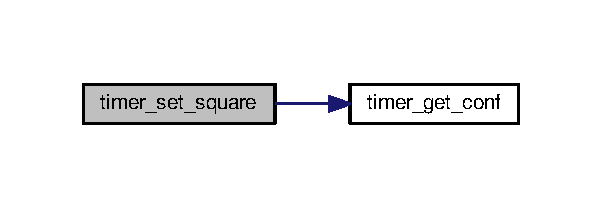
\includegraphics[width=289pt]{group__timer_gada4efbb5c88275795526fc45f0814aa3_cgraph}
\end{center}
\end{figure}


\index{timer@{timer}!timer\+\_\+subscribe\+\_\+int@{timer\+\_\+subscribe\+\_\+int}}
\index{timer\+\_\+subscribe\+\_\+int@{timer\+\_\+subscribe\+\_\+int}!timer@{timer}}
\subsubsection[{\texorpdfstring{timer\+\_\+subscribe\+\_\+int(void)}{timer_subscribe_int(void)}}]{\setlength{\rightskip}{0pt plus 5cm}int timer\+\_\+subscribe\+\_\+int (
\begin{DoxyParamCaption}
\item[{void}]{}
\end{DoxyParamCaption}
)}\hypertarget{group__timer_ga4c5d9f47323eda494cfd826f6d62eec9}{}\label{group__timer_ga4c5d9f47323eda494cfd826f6d62eec9}


Subscribes and enables Timer 0 interrupts. 

\begin{DoxyReturn}{Returns}
Returns bit order in interrupt mask; negative value on failure 
\end{DoxyReturn}
\index{timer@{timer}!timer\+\_\+test\+\_\+config@{timer\+\_\+test\+\_\+config}}
\index{timer\+\_\+test\+\_\+config@{timer\+\_\+test\+\_\+config}!timer@{timer}}
\subsubsection[{\texorpdfstring{timer\+\_\+test\+\_\+config(unsigned long timer)}{timer_test_config(unsigned long timer)}}]{\setlength{\rightskip}{0pt plus 5cm}int timer\+\_\+test\+\_\+config (
\begin{DoxyParamCaption}
\item[{unsigned long}]{timer}
\end{DoxyParamCaption}
)}\hypertarget{group__timer_ga363e72d1c055d859746cb3305a68af6d}{}\label{group__timer_ga363e72d1c055d859746cb3305a68af6d}


Tests display of timer config. 

Just calls \hyperlink{group__timer_ga8eb3357bc05265afc4bea5bbbb480a53}{timer\+\_\+get\+\_\+conf()} followed by \hyperlink{group__timer_ga9ca64a3f3f048936d961d656d6829200}{timer\+\_\+display\+\_\+conf()}


\begin{DoxyParams}{Parameters}
{\em timer} & Timer whose config to read (Ranges from 0 to 2) \\
\hline
\end{DoxyParams}
\begin{DoxyReturn}{Returns}
Return 0 upon success and non-\/zero otherwise 
\end{DoxyReturn}


Here is the call graph for this function\+:
\nopagebreak
\begin{figure}[H]
\begin{center}
\leavevmode
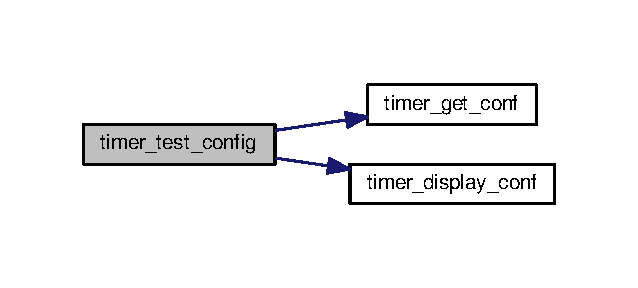
\includegraphics[width=306pt]{group__timer_ga363e72d1c055d859746cb3305a68af6d_cgraph}
\end{center}
\end{figure}


\index{timer@{timer}!timer\+\_\+test\+\_\+int@{timer\+\_\+test\+\_\+int}}
\index{timer\+\_\+test\+\_\+int@{timer\+\_\+test\+\_\+int}!timer@{timer}}
\subsubsection[{\texorpdfstring{timer\+\_\+test\+\_\+int(unsigned long time)}{timer_test_int(unsigned long time)}}]{\setlength{\rightskip}{0pt plus 5cm}int timer\+\_\+test\+\_\+int (
\begin{DoxyParamCaption}
\item[{unsigned long}]{time}
\end{DoxyParamCaption}
)}\hypertarget{group__timer_ga459859709b7cc1ee37899fa48cce6a6e}{}\label{group__timer_ga459859709b7cc1ee37899fa48cce6a6e}


Tests Timer 0 interrupt handling. 

Subscribes Timer 0 interrupts and prints a message once per second for the specified time interval


\begin{DoxyParams}{Parameters}
{\em time} & Length of time interval while interrupts are subscribed \\
\hline
\end{DoxyParams}
\begin{DoxyReturn}{Returns}
Return 0 upon success and non-\/zero otherwise 
\end{DoxyReturn}


Here is the call graph for this function\+:
\nopagebreak
\begin{figure}[H]
\begin{center}
\leavevmode
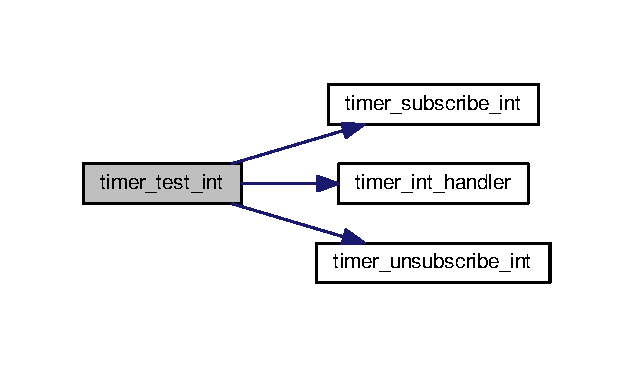
\includegraphics[width=304pt]{group__timer_ga459859709b7cc1ee37899fa48cce6a6e_cgraph}
\end{center}
\end{figure}


\index{timer@{timer}!timer\+\_\+test\+\_\+square@{timer\+\_\+test\+\_\+square}}
\index{timer\+\_\+test\+\_\+square@{timer\+\_\+test\+\_\+square}!timer@{timer}}
\subsubsection[{\texorpdfstring{timer\+\_\+test\+\_\+square(unsigned long freq)}{timer_test_square(unsigned long freq)}}]{\setlength{\rightskip}{0pt plus 5cm}int timer\+\_\+test\+\_\+square (
\begin{DoxyParamCaption}
\item[{unsigned long}]{freq}
\end{DoxyParamCaption}
)}\hypertarget{group__timer_ga2e596aede5a7bfc4a6f4382779bf0d7d}{}\label{group__timer_ga2e596aede5a7bfc4a6f4382779bf0d7d}


Tests programming timer in square wave mode. 

Programs Timer 0 to generate square mode with input frequency


\begin{DoxyParams}{Parameters}
{\em freq} & Frequency of square wave to generate \\
\hline
\end{DoxyParams}
\begin{DoxyReturn}{Returns}
Return 0 upon success and non-\/zero otherwise 
\end{DoxyReturn}


Here is the call graph for this function\+:
\nopagebreak
\begin{figure}[H]
\begin{center}
\leavevmode
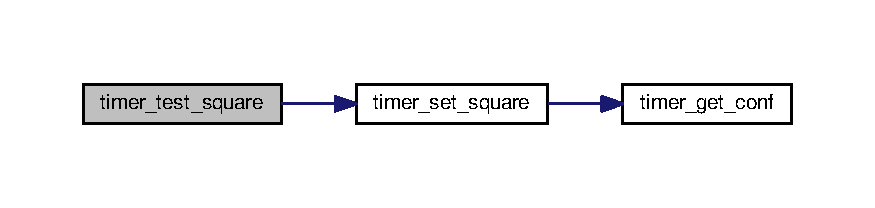
\includegraphics[width=350pt]{group__timer_ga2e596aede5a7bfc4a6f4382779bf0d7d_cgraph}
\end{center}
\end{figure}


\index{timer@{timer}!timer\+\_\+unsubscribe\+\_\+int@{timer\+\_\+unsubscribe\+\_\+int}}
\index{timer\+\_\+unsubscribe\+\_\+int@{timer\+\_\+unsubscribe\+\_\+int}!timer@{timer}}
\subsubsection[{\texorpdfstring{timer\+\_\+unsubscribe\+\_\+int()}{timer_unsubscribe_int()}}]{\setlength{\rightskip}{0pt plus 5cm}int timer\+\_\+unsubscribe\+\_\+int (
\begin{DoxyParamCaption}
{}
\end{DoxyParamCaption}
)}\hypertarget{group__timer_gab9eea51549744bca5c5c923b388bb4ee}{}\label{group__timer_gab9eea51549744bca5c5c923b388bb4ee}


Unsubscribes Timer 0 interrupts. 

\begin{DoxyReturn}{Returns}
Return 0 upon success and non-\/zero otherwise 
\end{DoxyReturn}

\hypertarget{group__vbe}{}\section{vbe}
\label{group__vbe}\index{vbe@{vbe}}
\subsection*{Classes}
\begin{DoxyCompactItemize}
\item 
struct \hyperlink{struct____attribute____}{\+\_\+\+\_\+attribute\+\_\+\+\_\+}
\end{DoxyCompactItemize}
\subsection*{Functions}
\begin{DoxyCompactItemize}
\item 
int \hyperlink{group__vbe_ga4ef3234e41f2050bc094a22049b69e45}{vbe\+\_\+get\+\_\+mode\+\_\+info} (unsigned short mode, vbe\+\_\+mode\+\_\+info\+\_\+t $\ast$vmi\+\_\+p)
\begin{DoxyCompactList}\small\item\em Returns information on the input V\+BE mode, including screen dimensions, color depth and V\+R\+AM physical address. \end{DoxyCompactList}\item 
int \hyperlink{group__vbe_gabd49ec69d3108f1379f668112ac8744b}{vbe\+\_\+read\+\_\+block\+\_\+info} (Vbe\+Info\+Block $\ast$vbp)
\end{DoxyCompactItemize}


\subsection{Detailed Description}
Functions related to the V\+BE standard 

\subsection{Function Documentation}
\index{vbe@{vbe}!vbe\+\_\+get\+\_\+mode\+\_\+info@{vbe\+\_\+get\+\_\+mode\+\_\+info}}
\index{vbe\+\_\+get\+\_\+mode\+\_\+info@{vbe\+\_\+get\+\_\+mode\+\_\+info}!vbe@{vbe}}
\subsubsection[{\texorpdfstring{vbe\+\_\+get\+\_\+mode\+\_\+info(unsigned short mode, vbe\+\_\+mode\+\_\+info\+\_\+t $\ast$vmi\+\_\+p)}{vbe_get_mode_info(unsigned short mode, vbe_mode_info_t *vmi_p)}}]{\setlength{\rightskip}{0pt plus 5cm}int vbe\+\_\+get\+\_\+mode\+\_\+info (
\begin{DoxyParamCaption}
\item[{unsigned short}]{mode, }
\item[{vbe\+\_\+mode\+\_\+info\+\_\+t $\ast$}]{vmi\+\_\+p}
\end{DoxyParamCaption}
)}\hypertarget{group__vbe_ga4ef3234e41f2050bc094a22049b69e45}{}\label{group__vbe_ga4ef3234e41f2050bc094a22049b69e45}


Returns information on the input V\+BE mode, including screen dimensions, color depth and V\+R\+AM physical address. 

Initializes unpacked vbe\+\_\+mode\+\_\+\+\_\+info\+\_\+t structure passed as an address with the information of the input mode, by calling V\+BE function 0x01 Return V\+BE Mode Information and unpacking the Mode\+Info\+Block struct returned by that function.


\begin{DoxyParams}{Parameters}
{\em mode} & mode whose information should be returned \\
\hline
{\em vmi\+\_\+p} & address of vbe\+\_\+mode\+\_\+info\+\_\+t structure to be initialized \\
\hline
\end{DoxyParams}
\begin{DoxyReturn}{Returns}
0 on success, non-\/zero otherwise 
\end{DoxyReturn}


Here is the call graph for this function\+:
\nopagebreak
\begin{figure}[H]
\begin{center}
\leavevmode
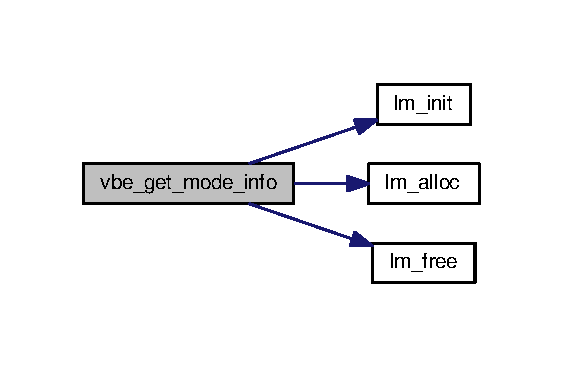
\includegraphics[width=270pt]{group__vbe_ga4ef3234e41f2050bc094a22049b69e45_cgraph}
\end{center}
\end{figure}


\index{vbe@{vbe}!vbe\+\_\+read\+\_\+block\+\_\+info@{vbe\+\_\+read\+\_\+block\+\_\+info}}
\index{vbe\+\_\+read\+\_\+block\+\_\+info@{vbe\+\_\+read\+\_\+block\+\_\+info}!vbe@{vbe}}
\subsubsection[{\texorpdfstring{vbe\+\_\+read\+\_\+block\+\_\+info(\+Vbe\+Info\+Block $\ast$vbp)}{vbe_read_block_info(VbeInfoBlock *vbp)}}]{\setlength{\rightskip}{0pt plus 5cm}int vbe\+\_\+read\+\_\+block\+\_\+info (
\begin{DoxyParamCaption}
\item[{Vbe\+Info\+Block $\ast$}]{vbp}
\end{DoxyParamCaption}
)}\hypertarget{group__vbe_gabd49ec69d3108f1379f668112ac8744b}{}\label{group__vbe_gabd49ec69d3108f1379f668112ac8744b}


Here is the call graph for this function\+:
\nopagebreak
\begin{figure}[H]
\begin{center}
\leavevmode
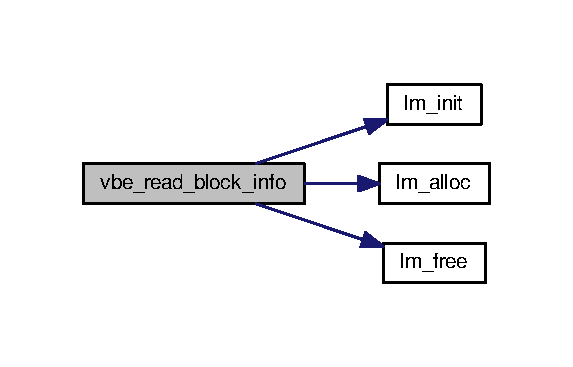
\includegraphics[width=275pt]{group__vbe_gabd49ec69d3108f1379f668112ac8744b_cgraph}
\end{center}
\end{figure}



\hypertarget{group__video__gr}{}\section{video\+\_\+gr}
\label{group__video__gr}\index{video\+\_\+gr@{video\+\_\+gr}}
\subsection*{Functions}
\begin{DoxyCompactItemize}
\item 
void $\ast$ \hyperlink{group__video__gr_gacef21667c79365d57a084bed994c2189}{vg\+\_\+init} (unsigned short mode)
\begin{DoxyCompactList}\small\item\em Initializes the video module in graphics mode. \end{DoxyCompactList}\item 
int \hyperlink{group__video__gr_ga42f593e6656f1a978315aff02b1bcebf}{vg\+\_\+exit} (void)
\begin{DoxyCompactList}\small\item\em Returns to default Minix 3 text mode (0x03\+: 25 x 80, 16 colors) \end{DoxyCompactList}\end{DoxyCompactItemize}


\subsection{Detailed Description}
Functions for outputing data to screen in graphics mode 

\subsection{Function Documentation}
\index{video\+\_\+gr@{video\+\_\+gr}!vg\+\_\+exit@{vg\+\_\+exit}}
\index{vg\+\_\+exit@{vg\+\_\+exit}!video\+\_\+gr@{video\+\_\+gr}}
\subsubsection[{\texorpdfstring{vg\+\_\+exit(void)}{vg_exit(void)}}]{\setlength{\rightskip}{0pt plus 5cm}int vg\+\_\+exit (
\begin{DoxyParamCaption}
\item[{void}]{}
\end{DoxyParamCaption}
)}\hypertarget{group__video__gr_ga42f593e6656f1a978315aff02b1bcebf}{}\label{group__video__gr_ga42f593e6656f1a978315aff02b1bcebf}


Returns to default Minix 3 text mode (0x03\+: 25 x 80, 16 colors) 

\begin{DoxyReturn}{Returns}
0 upon success, non-\/zero upon failure 
\end{DoxyReturn}
\index{video\+\_\+gr@{video\+\_\+gr}!vg\+\_\+init@{vg\+\_\+init}}
\index{vg\+\_\+init@{vg\+\_\+init}!video\+\_\+gr@{video\+\_\+gr}}
\subsubsection[{\texorpdfstring{vg\+\_\+init(unsigned short mode)}{vg_init(unsigned short mode)}}]{\setlength{\rightskip}{0pt plus 5cm}void$\ast$ vg\+\_\+init (
\begin{DoxyParamCaption}
\item[{unsigned short}]{mode}
\end{DoxyParamCaption}
)}\hypertarget{group__video__gr_gacef21667c79365d57a084bed994c2189}{}\label{group__video__gr_gacef21667c79365d57a084bed994c2189}


Initializes the video module in graphics mode. 

Uses the V\+BE I\+NT 0x10 interface to set the desired graphics mode, maps V\+R\+AM to the process\textquotesingle{} address space and initializes static global variables with the resolution of the screen, and the number of colors


\begin{DoxyParams}{Parameters}
{\em mode} & 16-\/bit V\+BE mode to set \\
\hline
\end{DoxyParams}
\begin{DoxyReturn}{Returns}
Virtual address V\+R\+AM was mapped to. N\+U\+LL, upon failure.
\end{DoxyReturn}
Uses the V\+BE I\+NT 0x10 interface to set the desired graphics mode, maps V\+R\+AM to the process\textquotesingle{} address space and initializes global variables with the resolution of the screen, and the number of colors


\begin{DoxyParams}{Parameters}
{\em mode} & 16-\/bit V\+BE mode to set \\
\hline
\end{DoxyParams}
\begin{DoxyReturn}{Returns}
Virtual address V\+R\+AM was mapped to. N\+U\+LL, upon failure. 
\end{DoxyReturn}


Here is the call graph for this function\+:
\nopagebreak
\begin{figure}[H]
\begin{center}
\leavevmode
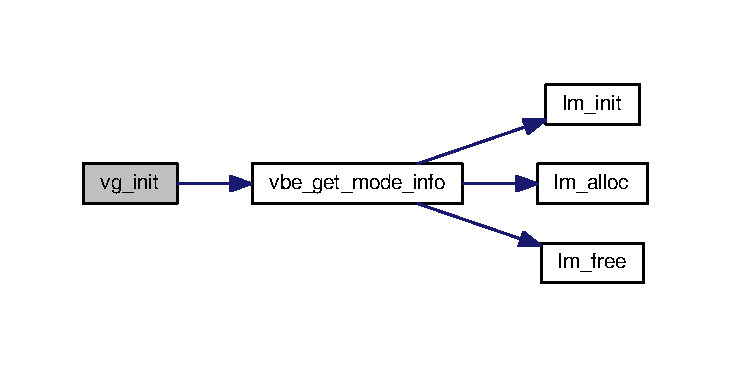
\includegraphics[width=350pt]{group__video__gr_gacef21667c79365d57a084bed994c2189_cgraph}
\end{center}
\end{figure}



\chapter{Class Documentation}
\hypertarget{struct____attribute____}{}\section{\+\_\+\+\_\+attribute\+\_\+\+\_\+ Struct Reference}
\label{struct____attribute____}\index{\+\_\+\+\_\+attribute\+\_\+\+\_\+@{\+\_\+\+\_\+attribute\+\_\+\+\_\+}}


{\ttfamily \#include $<$vbe.\+h$>$}

\subsection*{Public Attributes}
\begin{DoxyCompactItemize}
\item 
uint16\+\_\+t \hyperlink{struct____attribute_____a68ea99ad36679e583fa9674016e30903}{Mode\+Attributes}
\begin{DoxyCompactList}\small\item\em mode attributes \end{DoxyCompactList}\item 
uint8\+\_\+t \hyperlink{struct____attribute_____aeffe4dec59c5a757f65a97a66c812d3b}{Win\+A\+Attributes}
\begin{DoxyCompactList}\small\item\em window A attributes \end{DoxyCompactList}\item 
uint8\+\_\+t \hyperlink{struct____attribute_____ac9e21a3d7d22b24ed82be39f790b1408}{Win\+B\+Attributes}
\begin{DoxyCompactList}\small\item\em window B attributes \end{DoxyCompactList}\item 
uint16\+\_\+t \hyperlink{struct____attribute_____acc2114dbf039909e55cc3966abd3358d}{Win\+Granularity}
\begin{DoxyCompactList}\small\item\em window granularity \end{DoxyCompactList}\item 
uint16\+\_\+t \hyperlink{struct____attribute_____ad26e754fe362f3085c7ec4c0e5e75a6f}{Win\+Size}
\begin{DoxyCompactList}\small\item\em window size \end{DoxyCompactList}\item 
uint16\+\_\+t \hyperlink{struct____attribute_____a7cde26f911e3df97b7498ee139d8de12}{Win\+A\+Segment}
\begin{DoxyCompactList}\small\item\em window A start segment \end{DoxyCompactList}\item 
uint16\+\_\+t \hyperlink{struct____attribute_____a6dbaac9ee1cae36ca0c7b46559264b69}{Win\+B\+Segment}
\begin{DoxyCompactList}\small\item\em window B start segment \end{DoxyCompactList}\item 
phys\+\_\+bytes \hyperlink{struct____attribute_____aa211c2411f48f899b0bb0739ecef0b37}{Win\+Func\+Ptr}
\begin{DoxyCompactList}\small\item\em real mode/far pointer to window function \end{DoxyCompactList}\item 
uint16\+\_\+t \hyperlink{struct____attribute_____a3c9eb4b107ecee102c6e63f9054ede06}{Bytes\+Per\+Scan\+Line}
\begin{DoxyCompactList}\small\item\em bytes per scan line \end{DoxyCompactList}\item 
uint16\+\_\+t \hyperlink{struct____attribute_____abe48e2b29aa99e813a1447d22711f4f4}{X\+Resolution}
\begin{DoxyCompactList}\small\item\em horizontal resolution in pixels/characters \end{DoxyCompactList}\item 
uint16\+\_\+t \hyperlink{struct____attribute_____aa91385451d974d9c33978062e22d39e2}{Y\+Resolution}
\begin{DoxyCompactList}\small\item\em vertical resolution in pixels/characters \end{DoxyCompactList}\item 
uint8\+\_\+t \hyperlink{struct____attribute_____acac41a300563737d7849a92cd1d5c10b}{X\+Char\+Size}
\begin{DoxyCompactList}\small\item\em character cell width in pixels \end{DoxyCompactList}\item 
uint8\+\_\+t \hyperlink{struct____attribute_____acb93d86860efea5c87e3c2950f39123e}{Y\+Char\+Size}
\begin{DoxyCompactList}\small\item\em character cell height in pixels \end{DoxyCompactList}\item 
uint8\+\_\+t \hyperlink{struct____attribute_____ab1471d2f75e61117d65290da9070cf89}{Number\+Of\+Planes}
\begin{DoxyCompactList}\small\item\em number of memory planes \end{DoxyCompactList}\item 
uint8\+\_\+t \hyperlink{struct____attribute_____abd9c59af53589a54188bb57ada5c5f26}{Bits\+Per\+Pixel}
\begin{DoxyCompactList}\small\item\em bits per pixel \end{DoxyCompactList}\item 
uint8\+\_\+t \hyperlink{struct____attribute_____a59483378dd87414afcde6cb3ca93c2d8}{Number\+Of\+Banks}
\begin{DoxyCompactList}\small\item\em number of banks \end{DoxyCompactList}\item 
uint8\+\_\+t \hyperlink{struct____attribute_____a0fe34321b6dfba9e784fbbc649aa193a}{Memory\+Model}
\begin{DoxyCompactList}\small\item\em memory model type \end{DoxyCompactList}\item 
uint8\+\_\+t \hyperlink{struct____attribute_____aa1307567cbc12f9c5c724b7457be14ad}{Bank\+Size}
\begin{DoxyCompactList}\small\item\em bank size in KB \end{DoxyCompactList}\item 
uint8\+\_\+t \hyperlink{struct____attribute_____a988714bc16626547fbdc31f25dfa6470}{Number\+Of\+Image\+Pages}
\begin{DoxyCompactList}\small\item\em number of images \end{DoxyCompactList}\item 
uint8\+\_\+t \hyperlink{struct____attribute_____a8ace2dfe4814abc401442986ac8a5356}{Reserved1}
\begin{DoxyCompactList}\small\item\em reserved for page function \end{DoxyCompactList}\item 
uint8\+\_\+t \hyperlink{struct____attribute_____a9ffc14e11d6b1c80b63aba344292849e}{Red\+Mask\+Size}
\item 
uint8\+\_\+t \hyperlink{struct____attribute_____a8b5b2e458757061bce7e056f7f910dae}{Red\+Field\+Position}
\item 
uint8\+\_\+t \hyperlink{struct____attribute_____af69ef188a0f5d526ecd5f25a8d6336e3}{Green\+Mask\+Size}
\item 
uint8\+\_\+t \hyperlink{struct____attribute_____a44aab7c8026a131654e079837a95ba2b}{Green\+Field\+Position}
\item 
uint8\+\_\+t \hyperlink{struct____attribute_____ab5967602a79dcb7f0061195ffdaaa47a}{Blue\+Mask\+Size}
\item 
uint8\+\_\+t \hyperlink{struct____attribute_____ada852d5ed926757d24b5038a38e6292c}{Blue\+Field\+Position}
\item 
uint8\+\_\+t \hyperlink{struct____attribute_____a73862db83bdb9b6d31356af3cec7a5be}{Rsvd\+Mask\+Size}
\item 
uint8\+\_\+t \hyperlink{struct____attribute_____a61fb6dc07b7edbd8a3a94745336f256c}{Rsvd\+Field\+Position}
\item 
uint8\+\_\+t \hyperlink{struct____attribute_____a35fb3e1fc0dc9924bc52977b3a234f9f}{Direct\+Color\+Mode\+Info}
\item 
phys\+\_\+bytes \hyperlink{struct____attribute_____a852a4f68cfbabf08df197128e137bde6}{Phys\+Base\+Ptr}
\begin{DoxyCompactList}\small\item\em physical address for flat memory frame buffer \end{DoxyCompactList}\item 
uint8\+\_\+t \hyperlink{struct____attribute_____a534ebf7a2bdad17747cfc9cb6cc50c5c}{Reserved2} \mbox{[}4\mbox{]}
\begin{DoxyCompactList}\small\item\em Reserved -\/ always set to 0. \end{DoxyCompactList}\item 
uint8\+\_\+t \hyperlink{struct____attribute_____a9336499af9094522dbe1bfd4d43934a1}{Reserved3} \mbox{[}2\mbox{]}
\begin{DoxyCompactList}\small\item\em Reserved -\/ always set to 0. \end{DoxyCompactList}\item 
uint16\+\_\+t \hyperlink{struct____attribute_____af7036270c257deabc1ebd111faf3e3a5}{Lin\+Bytes\+Per\+Scan\+Line}
\item 
uint8\+\_\+t \hyperlink{struct____attribute_____ad5820084f2b821b85a635df8394f0d9e}{Bnk\+Number\+Of\+Image\+Pages}
\item 
uint8\+\_\+t \hyperlink{struct____attribute_____af9ba0d9902f5336bd9d044a9dee2ba42}{Lin\+Number\+Of\+Image\+Pages}
\item 
uint8\+\_\+t \hyperlink{struct____attribute_____a88a5ced225c9ef7ed6ffe33e5a39edc6}{Lin\+Red\+Mask\+Size}
\item 
uint8\+\_\+t \hyperlink{struct____attribute_____aec8d45f188ac9210b88216af83de847d}{Lin\+Red\+Field\+Position}
\item 
uint8\+\_\+t \hyperlink{struct____attribute_____a5768a84391f8a26d8a9bfd6a22d5e49d}{Lin\+Green\+Mask\+Size}
\item 
uint8\+\_\+t \hyperlink{struct____attribute_____a5571b1959950d520f2b45bb5549994e3}{Lin\+Green\+Field\+Position}
\item 
uint8\+\_\+t \hyperlink{struct____attribute_____aa2b79b8eed8d842e0db481fb1fbb9a06}{Lin\+Blue\+Mask\+Size}
\item 
uint8\+\_\+t \hyperlink{struct____attribute_____a99e6b6bdbda9f98f2823429dfd5b5685}{Lin\+Blue\+Field\+Position}
\item 
uint8\+\_\+t \hyperlink{struct____attribute_____a577b5892a22d06e230f528a62a472d1d}{Lin\+Rsvd\+Mask\+Size}
\item 
uint8\+\_\+t \hyperlink{struct____attribute_____a012126db503ad1281ae53aa41f4c96a7}{Lin\+Rsvd\+Field\+Position}
\item 
uint32\+\_\+t \hyperlink{struct____attribute_____afd81a69353c35e8b1fb9b696931f79a5}{Max\+Pixel\+Clock}
\item 
uint8\+\_\+t \hyperlink{struct____attribute_____ab859fb715f83f005dfa2f13d8b0e4ff0}{Reserved4} \mbox{[}190\mbox{]}
\item 
char \hyperlink{struct____attribute_____a9f5c2950d459303bbc740109d3e0c474}{Vbe\+Signature} \mbox{[}4\mbox{]}
\item 
uint16\+\_\+t \hyperlink{struct____attribute_____ab50a7a6ed578c30d9411db043c0b34c9}{Vbe\+Version}
\item 
uint16\+\_\+t \hyperlink{struct____attribute_____a5a097456359234e9d2ed119aec00fba4}{Oem\+String\+Ptr} \mbox{[}2\mbox{]}
\item 
uint8\+\_\+t \hyperlink{struct____attribute_____a03972171b961723d316eb382e40a7409}{Capabilities} \mbox{[}4\mbox{]}
\item 
uint16\+\_\+t \hyperlink{struct____attribute_____a135a4de316befee6c1415c22e5636f15}{Video\+Mode\+Ptr} \mbox{[}2\mbox{]}
\item 
uint16\+\_\+t \hyperlink{struct____attribute_____a5659e88b961bf423d6385f315264e005}{Total\+Memory}
\end{DoxyCompactItemize}


\subsection{Detailed Description}
Packed V\+BE Mode Info Block 

\subsection{Member Data Documentation}
\index{\+\_\+\+\_\+attribute\+\_\+\+\_\+@{\+\_\+\+\_\+attribute\+\_\+\+\_\+}!Bank\+Size@{Bank\+Size}}
\index{Bank\+Size@{Bank\+Size}!\+\_\+\+\_\+attribute\+\_\+\+\_\+@{\+\_\+\+\_\+attribute\+\_\+\+\_\+}}
\subsubsection[{\texorpdfstring{Bank\+Size}{BankSize}}]{\setlength{\rightskip}{0pt plus 5cm}uint8\+\_\+t \+\_\+\+\_\+attribute\+\_\+\+\_\+\+::\+Bank\+Size}\hypertarget{struct____attribute_____aa1307567cbc12f9c5c724b7457be14ad}{}\label{struct____attribute_____aa1307567cbc12f9c5c724b7457be14ad}


bank size in KB 

\index{\+\_\+\+\_\+attribute\+\_\+\+\_\+@{\+\_\+\+\_\+attribute\+\_\+\+\_\+}!Bits\+Per\+Pixel@{Bits\+Per\+Pixel}}
\index{Bits\+Per\+Pixel@{Bits\+Per\+Pixel}!\+\_\+\+\_\+attribute\+\_\+\+\_\+@{\+\_\+\+\_\+attribute\+\_\+\+\_\+}}
\subsubsection[{\texorpdfstring{Bits\+Per\+Pixel}{BitsPerPixel}}]{\setlength{\rightskip}{0pt plus 5cm}uint8\+\_\+t \+\_\+\+\_\+attribute\+\_\+\+\_\+\+::\+Bits\+Per\+Pixel}\hypertarget{struct____attribute_____abd9c59af53589a54188bb57ada5c5f26}{}\label{struct____attribute_____abd9c59af53589a54188bb57ada5c5f26}


bits per pixel 

\index{\+\_\+\+\_\+attribute\+\_\+\+\_\+@{\+\_\+\+\_\+attribute\+\_\+\+\_\+}!Blue\+Field\+Position@{Blue\+Field\+Position}}
\index{Blue\+Field\+Position@{Blue\+Field\+Position}!\+\_\+\+\_\+attribute\+\_\+\+\_\+@{\+\_\+\+\_\+attribute\+\_\+\+\_\+}}
\subsubsection[{\texorpdfstring{Blue\+Field\+Position}{BlueFieldPosition}}]{\setlength{\rightskip}{0pt plus 5cm}uint8\+\_\+t \+\_\+\+\_\+attribute\+\_\+\+\_\+\+::\+Blue\+Field\+Position}\hypertarget{struct____attribute_____ada852d5ed926757d24b5038a38e6292c}{}\label{struct____attribute_____ada852d5ed926757d24b5038a38e6292c}
\index{\+\_\+\+\_\+attribute\+\_\+\+\_\+@{\+\_\+\+\_\+attribute\+\_\+\+\_\+}!Blue\+Mask\+Size@{Blue\+Mask\+Size}}
\index{Blue\+Mask\+Size@{Blue\+Mask\+Size}!\+\_\+\+\_\+attribute\+\_\+\+\_\+@{\+\_\+\+\_\+attribute\+\_\+\+\_\+}}
\subsubsection[{\texorpdfstring{Blue\+Mask\+Size}{BlueMaskSize}}]{\setlength{\rightskip}{0pt plus 5cm}uint8\+\_\+t \+\_\+\+\_\+attribute\+\_\+\+\_\+\+::\+Blue\+Mask\+Size}\hypertarget{struct____attribute_____ab5967602a79dcb7f0061195ffdaaa47a}{}\label{struct____attribute_____ab5967602a79dcb7f0061195ffdaaa47a}
\index{\+\_\+\+\_\+attribute\+\_\+\+\_\+@{\+\_\+\+\_\+attribute\+\_\+\+\_\+}!Bnk\+Number\+Of\+Image\+Pages@{Bnk\+Number\+Of\+Image\+Pages}}
\index{Bnk\+Number\+Of\+Image\+Pages@{Bnk\+Number\+Of\+Image\+Pages}!\+\_\+\+\_\+attribute\+\_\+\+\_\+@{\+\_\+\+\_\+attribute\+\_\+\+\_\+}}
\subsubsection[{\texorpdfstring{Bnk\+Number\+Of\+Image\+Pages}{BnkNumberOfImagePages}}]{\setlength{\rightskip}{0pt plus 5cm}uint8\+\_\+t \+\_\+\+\_\+attribute\+\_\+\+\_\+\+::\+Bnk\+Number\+Of\+Image\+Pages}\hypertarget{struct____attribute_____ad5820084f2b821b85a635df8394f0d9e}{}\label{struct____attribute_____ad5820084f2b821b85a635df8394f0d9e}
\index{\+\_\+\+\_\+attribute\+\_\+\+\_\+@{\+\_\+\+\_\+attribute\+\_\+\+\_\+}!Bytes\+Per\+Scan\+Line@{Bytes\+Per\+Scan\+Line}}
\index{Bytes\+Per\+Scan\+Line@{Bytes\+Per\+Scan\+Line}!\+\_\+\+\_\+attribute\+\_\+\+\_\+@{\+\_\+\+\_\+attribute\+\_\+\+\_\+}}
\subsubsection[{\texorpdfstring{Bytes\+Per\+Scan\+Line}{BytesPerScanLine}}]{\setlength{\rightskip}{0pt plus 5cm}uint16\+\_\+t \+\_\+\+\_\+attribute\+\_\+\+\_\+\+::\+Bytes\+Per\+Scan\+Line}\hypertarget{struct____attribute_____a3c9eb4b107ecee102c6e63f9054ede06}{}\label{struct____attribute_____a3c9eb4b107ecee102c6e63f9054ede06}


bytes per scan line 

\index{\+\_\+\+\_\+attribute\+\_\+\+\_\+@{\+\_\+\+\_\+attribute\+\_\+\+\_\+}!Capabilities@{Capabilities}}
\index{Capabilities@{Capabilities}!\+\_\+\+\_\+attribute\+\_\+\+\_\+@{\+\_\+\+\_\+attribute\+\_\+\+\_\+}}
\subsubsection[{\texorpdfstring{Capabilities}{Capabilities}}]{\setlength{\rightskip}{0pt plus 5cm}uint8\+\_\+t \+\_\+\+\_\+attribute\+\_\+\+\_\+\+::\+Capabilities\mbox{[}4\mbox{]}}\hypertarget{struct____attribute_____a03972171b961723d316eb382e40a7409}{}\label{struct____attribute_____a03972171b961723d316eb382e40a7409}
\index{\+\_\+\+\_\+attribute\+\_\+\+\_\+@{\+\_\+\+\_\+attribute\+\_\+\+\_\+}!Direct\+Color\+Mode\+Info@{Direct\+Color\+Mode\+Info}}
\index{Direct\+Color\+Mode\+Info@{Direct\+Color\+Mode\+Info}!\+\_\+\+\_\+attribute\+\_\+\+\_\+@{\+\_\+\+\_\+attribute\+\_\+\+\_\+}}
\subsubsection[{\texorpdfstring{Direct\+Color\+Mode\+Info}{DirectColorModeInfo}}]{\setlength{\rightskip}{0pt plus 5cm}uint8\+\_\+t \+\_\+\+\_\+attribute\+\_\+\+\_\+\+::\+Direct\+Color\+Mode\+Info}\hypertarget{struct____attribute_____a35fb3e1fc0dc9924bc52977b3a234f9f}{}\label{struct____attribute_____a35fb3e1fc0dc9924bc52977b3a234f9f}
\index{\+\_\+\+\_\+attribute\+\_\+\+\_\+@{\+\_\+\+\_\+attribute\+\_\+\+\_\+}!Green\+Field\+Position@{Green\+Field\+Position}}
\index{Green\+Field\+Position@{Green\+Field\+Position}!\+\_\+\+\_\+attribute\+\_\+\+\_\+@{\+\_\+\+\_\+attribute\+\_\+\+\_\+}}
\subsubsection[{\texorpdfstring{Green\+Field\+Position}{GreenFieldPosition}}]{\setlength{\rightskip}{0pt plus 5cm}uint8\+\_\+t \+\_\+\+\_\+attribute\+\_\+\+\_\+\+::\+Green\+Field\+Position}\hypertarget{struct____attribute_____a44aab7c8026a131654e079837a95ba2b}{}\label{struct____attribute_____a44aab7c8026a131654e079837a95ba2b}
\index{\+\_\+\+\_\+attribute\+\_\+\+\_\+@{\+\_\+\+\_\+attribute\+\_\+\+\_\+}!Green\+Mask\+Size@{Green\+Mask\+Size}}
\index{Green\+Mask\+Size@{Green\+Mask\+Size}!\+\_\+\+\_\+attribute\+\_\+\+\_\+@{\+\_\+\+\_\+attribute\+\_\+\+\_\+}}
\subsubsection[{\texorpdfstring{Green\+Mask\+Size}{GreenMaskSize}}]{\setlength{\rightskip}{0pt plus 5cm}uint8\+\_\+t \+\_\+\+\_\+attribute\+\_\+\+\_\+\+::\+Green\+Mask\+Size}\hypertarget{struct____attribute_____af69ef188a0f5d526ecd5f25a8d6336e3}{}\label{struct____attribute_____af69ef188a0f5d526ecd5f25a8d6336e3}
\index{\+\_\+\+\_\+attribute\+\_\+\+\_\+@{\+\_\+\+\_\+attribute\+\_\+\+\_\+}!Lin\+Blue\+Field\+Position@{Lin\+Blue\+Field\+Position}}
\index{Lin\+Blue\+Field\+Position@{Lin\+Blue\+Field\+Position}!\+\_\+\+\_\+attribute\+\_\+\+\_\+@{\+\_\+\+\_\+attribute\+\_\+\+\_\+}}
\subsubsection[{\texorpdfstring{Lin\+Blue\+Field\+Position}{LinBlueFieldPosition}}]{\setlength{\rightskip}{0pt plus 5cm}uint8\+\_\+t \+\_\+\+\_\+attribute\+\_\+\+\_\+\+::\+Lin\+Blue\+Field\+Position}\hypertarget{struct____attribute_____a99e6b6bdbda9f98f2823429dfd5b5685}{}\label{struct____attribute_____a99e6b6bdbda9f98f2823429dfd5b5685}
\index{\+\_\+\+\_\+attribute\+\_\+\+\_\+@{\+\_\+\+\_\+attribute\+\_\+\+\_\+}!Lin\+Blue\+Mask\+Size@{Lin\+Blue\+Mask\+Size}}
\index{Lin\+Blue\+Mask\+Size@{Lin\+Blue\+Mask\+Size}!\+\_\+\+\_\+attribute\+\_\+\+\_\+@{\+\_\+\+\_\+attribute\+\_\+\+\_\+}}
\subsubsection[{\texorpdfstring{Lin\+Blue\+Mask\+Size}{LinBlueMaskSize}}]{\setlength{\rightskip}{0pt plus 5cm}uint8\+\_\+t \+\_\+\+\_\+attribute\+\_\+\+\_\+\+::\+Lin\+Blue\+Mask\+Size}\hypertarget{struct____attribute_____aa2b79b8eed8d842e0db481fb1fbb9a06}{}\label{struct____attribute_____aa2b79b8eed8d842e0db481fb1fbb9a06}
\index{\+\_\+\+\_\+attribute\+\_\+\+\_\+@{\+\_\+\+\_\+attribute\+\_\+\+\_\+}!Lin\+Bytes\+Per\+Scan\+Line@{Lin\+Bytes\+Per\+Scan\+Line}}
\index{Lin\+Bytes\+Per\+Scan\+Line@{Lin\+Bytes\+Per\+Scan\+Line}!\+\_\+\+\_\+attribute\+\_\+\+\_\+@{\+\_\+\+\_\+attribute\+\_\+\+\_\+}}
\subsubsection[{\texorpdfstring{Lin\+Bytes\+Per\+Scan\+Line}{LinBytesPerScanLine}}]{\setlength{\rightskip}{0pt plus 5cm}uint16\+\_\+t \+\_\+\+\_\+attribute\+\_\+\+\_\+\+::\+Lin\+Bytes\+Per\+Scan\+Line}\hypertarget{struct____attribute_____af7036270c257deabc1ebd111faf3e3a5}{}\label{struct____attribute_____af7036270c257deabc1ebd111faf3e3a5}
\index{\+\_\+\+\_\+attribute\+\_\+\+\_\+@{\+\_\+\+\_\+attribute\+\_\+\+\_\+}!Lin\+Green\+Field\+Position@{Lin\+Green\+Field\+Position}}
\index{Lin\+Green\+Field\+Position@{Lin\+Green\+Field\+Position}!\+\_\+\+\_\+attribute\+\_\+\+\_\+@{\+\_\+\+\_\+attribute\+\_\+\+\_\+}}
\subsubsection[{\texorpdfstring{Lin\+Green\+Field\+Position}{LinGreenFieldPosition}}]{\setlength{\rightskip}{0pt plus 5cm}uint8\+\_\+t \+\_\+\+\_\+attribute\+\_\+\+\_\+\+::\+Lin\+Green\+Field\+Position}\hypertarget{struct____attribute_____a5571b1959950d520f2b45bb5549994e3}{}\label{struct____attribute_____a5571b1959950d520f2b45bb5549994e3}
\index{\+\_\+\+\_\+attribute\+\_\+\+\_\+@{\+\_\+\+\_\+attribute\+\_\+\+\_\+}!Lin\+Green\+Mask\+Size@{Lin\+Green\+Mask\+Size}}
\index{Lin\+Green\+Mask\+Size@{Lin\+Green\+Mask\+Size}!\+\_\+\+\_\+attribute\+\_\+\+\_\+@{\+\_\+\+\_\+attribute\+\_\+\+\_\+}}
\subsubsection[{\texorpdfstring{Lin\+Green\+Mask\+Size}{LinGreenMaskSize}}]{\setlength{\rightskip}{0pt plus 5cm}uint8\+\_\+t \+\_\+\+\_\+attribute\+\_\+\+\_\+\+::\+Lin\+Green\+Mask\+Size}\hypertarget{struct____attribute_____a5768a84391f8a26d8a9bfd6a22d5e49d}{}\label{struct____attribute_____a5768a84391f8a26d8a9bfd6a22d5e49d}
\index{\+\_\+\+\_\+attribute\+\_\+\+\_\+@{\+\_\+\+\_\+attribute\+\_\+\+\_\+}!Lin\+Number\+Of\+Image\+Pages@{Lin\+Number\+Of\+Image\+Pages}}
\index{Lin\+Number\+Of\+Image\+Pages@{Lin\+Number\+Of\+Image\+Pages}!\+\_\+\+\_\+attribute\+\_\+\+\_\+@{\+\_\+\+\_\+attribute\+\_\+\+\_\+}}
\subsubsection[{\texorpdfstring{Lin\+Number\+Of\+Image\+Pages}{LinNumberOfImagePages}}]{\setlength{\rightskip}{0pt plus 5cm}uint8\+\_\+t \+\_\+\+\_\+attribute\+\_\+\+\_\+\+::\+Lin\+Number\+Of\+Image\+Pages}\hypertarget{struct____attribute_____af9ba0d9902f5336bd9d044a9dee2ba42}{}\label{struct____attribute_____af9ba0d9902f5336bd9d044a9dee2ba42}
\index{\+\_\+\+\_\+attribute\+\_\+\+\_\+@{\+\_\+\+\_\+attribute\+\_\+\+\_\+}!Lin\+Red\+Field\+Position@{Lin\+Red\+Field\+Position}}
\index{Lin\+Red\+Field\+Position@{Lin\+Red\+Field\+Position}!\+\_\+\+\_\+attribute\+\_\+\+\_\+@{\+\_\+\+\_\+attribute\+\_\+\+\_\+}}
\subsubsection[{\texorpdfstring{Lin\+Red\+Field\+Position}{LinRedFieldPosition}}]{\setlength{\rightskip}{0pt plus 5cm}uint8\+\_\+t \+\_\+\+\_\+attribute\+\_\+\+\_\+\+::\+Lin\+Red\+Field\+Position}\hypertarget{struct____attribute_____aec8d45f188ac9210b88216af83de847d}{}\label{struct____attribute_____aec8d45f188ac9210b88216af83de847d}
\index{\+\_\+\+\_\+attribute\+\_\+\+\_\+@{\+\_\+\+\_\+attribute\+\_\+\+\_\+}!Lin\+Red\+Mask\+Size@{Lin\+Red\+Mask\+Size}}
\index{Lin\+Red\+Mask\+Size@{Lin\+Red\+Mask\+Size}!\+\_\+\+\_\+attribute\+\_\+\+\_\+@{\+\_\+\+\_\+attribute\+\_\+\+\_\+}}
\subsubsection[{\texorpdfstring{Lin\+Red\+Mask\+Size}{LinRedMaskSize}}]{\setlength{\rightskip}{0pt plus 5cm}uint8\+\_\+t \+\_\+\+\_\+attribute\+\_\+\+\_\+\+::\+Lin\+Red\+Mask\+Size}\hypertarget{struct____attribute_____a88a5ced225c9ef7ed6ffe33e5a39edc6}{}\label{struct____attribute_____a88a5ced225c9ef7ed6ffe33e5a39edc6}
\index{\+\_\+\+\_\+attribute\+\_\+\+\_\+@{\+\_\+\+\_\+attribute\+\_\+\+\_\+}!Lin\+Rsvd\+Field\+Position@{Lin\+Rsvd\+Field\+Position}}
\index{Lin\+Rsvd\+Field\+Position@{Lin\+Rsvd\+Field\+Position}!\+\_\+\+\_\+attribute\+\_\+\+\_\+@{\+\_\+\+\_\+attribute\+\_\+\+\_\+}}
\subsubsection[{\texorpdfstring{Lin\+Rsvd\+Field\+Position}{LinRsvdFieldPosition}}]{\setlength{\rightskip}{0pt plus 5cm}uint8\+\_\+t \+\_\+\+\_\+attribute\+\_\+\+\_\+\+::\+Lin\+Rsvd\+Field\+Position}\hypertarget{struct____attribute_____a012126db503ad1281ae53aa41f4c96a7}{}\label{struct____attribute_____a012126db503ad1281ae53aa41f4c96a7}
\index{\+\_\+\+\_\+attribute\+\_\+\+\_\+@{\+\_\+\+\_\+attribute\+\_\+\+\_\+}!Lin\+Rsvd\+Mask\+Size@{Lin\+Rsvd\+Mask\+Size}}
\index{Lin\+Rsvd\+Mask\+Size@{Lin\+Rsvd\+Mask\+Size}!\+\_\+\+\_\+attribute\+\_\+\+\_\+@{\+\_\+\+\_\+attribute\+\_\+\+\_\+}}
\subsubsection[{\texorpdfstring{Lin\+Rsvd\+Mask\+Size}{LinRsvdMaskSize}}]{\setlength{\rightskip}{0pt plus 5cm}uint8\+\_\+t \+\_\+\+\_\+attribute\+\_\+\+\_\+\+::\+Lin\+Rsvd\+Mask\+Size}\hypertarget{struct____attribute_____a577b5892a22d06e230f528a62a472d1d}{}\label{struct____attribute_____a577b5892a22d06e230f528a62a472d1d}
\index{\+\_\+\+\_\+attribute\+\_\+\+\_\+@{\+\_\+\+\_\+attribute\+\_\+\+\_\+}!Max\+Pixel\+Clock@{Max\+Pixel\+Clock}}
\index{Max\+Pixel\+Clock@{Max\+Pixel\+Clock}!\+\_\+\+\_\+attribute\+\_\+\+\_\+@{\+\_\+\+\_\+attribute\+\_\+\+\_\+}}
\subsubsection[{\texorpdfstring{Max\+Pixel\+Clock}{MaxPixelClock}}]{\setlength{\rightskip}{0pt plus 5cm}uint32\+\_\+t \+\_\+\+\_\+attribute\+\_\+\+\_\+\+::\+Max\+Pixel\+Clock}\hypertarget{struct____attribute_____afd81a69353c35e8b1fb9b696931f79a5}{}\label{struct____attribute_____afd81a69353c35e8b1fb9b696931f79a5}
\index{\+\_\+\+\_\+attribute\+\_\+\+\_\+@{\+\_\+\+\_\+attribute\+\_\+\+\_\+}!Memory\+Model@{Memory\+Model}}
\index{Memory\+Model@{Memory\+Model}!\+\_\+\+\_\+attribute\+\_\+\+\_\+@{\+\_\+\+\_\+attribute\+\_\+\+\_\+}}
\subsubsection[{\texorpdfstring{Memory\+Model}{MemoryModel}}]{\setlength{\rightskip}{0pt plus 5cm}uint8\+\_\+t \+\_\+\+\_\+attribute\+\_\+\+\_\+\+::\+Memory\+Model}\hypertarget{struct____attribute_____a0fe34321b6dfba9e784fbbc649aa193a}{}\label{struct____attribute_____a0fe34321b6dfba9e784fbbc649aa193a}


memory model type 

\index{\+\_\+\+\_\+attribute\+\_\+\+\_\+@{\+\_\+\+\_\+attribute\+\_\+\+\_\+}!Mode\+Attributes@{Mode\+Attributes}}
\index{Mode\+Attributes@{Mode\+Attributes}!\+\_\+\+\_\+attribute\+\_\+\+\_\+@{\+\_\+\+\_\+attribute\+\_\+\+\_\+}}
\subsubsection[{\texorpdfstring{Mode\+Attributes}{ModeAttributes}}]{\setlength{\rightskip}{0pt plus 5cm}uint16\+\_\+t \+\_\+\+\_\+attribute\+\_\+\+\_\+\+::\+Mode\+Attributes}\hypertarget{struct____attribute_____a68ea99ad36679e583fa9674016e30903}{}\label{struct____attribute_____a68ea99ad36679e583fa9674016e30903}


mode attributes 

\index{\+\_\+\+\_\+attribute\+\_\+\+\_\+@{\+\_\+\+\_\+attribute\+\_\+\+\_\+}!Number\+Of\+Banks@{Number\+Of\+Banks}}
\index{Number\+Of\+Banks@{Number\+Of\+Banks}!\+\_\+\+\_\+attribute\+\_\+\+\_\+@{\+\_\+\+\_\+attribute\+\_\+\+\_\+}}
\subsubsection[{\texorpdfstring{Number\+Of\+Banks}{NumberOfBanks}}]{\setlength{\rightskip}{0pt plus 5cm}uint8\+\_\+t \+\_\+\+\_\+attribute\+\_\+\+\_\+\+::\+Number\+Of\+Banks}\hypertarget{struct____attribute_____a59483378dd87414afcde6cb3ca93c2d8}{}\label{struct____attribute_____a59483378dd87414afcde6cb3ca93c2d8}


number of banks 

\index{\+\_\+\+\_\+attribute\+\_\+\+\_\+@{\+\_\+\+\_\+attribute\+\_\+\+\_\+}!Number\+Of\+Image\+Pages@{Number\+Of\+Image\+Pages}}
\index{Number\+Of\+Image\+Pages@{Number\+Of\+Image\+Pages}!\+\_\+\+\_\+attribute\+\_\+\+\_\+@{\+\_\+\+\_\+attribute\+\_\+\+\_\+}}
\subsubsection[{\texorpdfstring{Number\+Of\+Image\+Pages}{NumberOfImagePages}}]{\setlength{\rightskip}{0pt plus 5cm}uint8\+\_\+t \+\_\+\+\_\+attribute\+\_\+\+\_\+\+::\+Number\+Of\+Image\+Pages}\hypertarget{struct____attribute_____a988714bc16626547fbdc31f25dfa6470}{}\label{struct____attribute_____a988714bc16626547fbdc31f25dfa6470}


number of images 

\index{\+\_\+\+\_\+attribute\+\_\+\+\_\+@{\+\_\+\+\_\+attribute\+\_\+\+\_\+}!Number\+Of\+Planes@{Number\+Of\+Planes}}
\index{Number\+Of\+Planes@{Number\+Of\+Planes}!\+\_\+\+\_\+attribute\+\_\+\+\_\+@{\+\_\+\+\_\+attribute\+\_\+\+\_\+}}
\subsubsection[{\texorpdfstring{Number\+Of\+Planes}{NumberOfPlanes}}]{\setlength{\rightskip}{0pt plus 5cm}uint8\+\_\+t \+\_\+\+\_\+attribute\+\_\+\+\_\+\+::\+Number\+Of\+Planes}\hypertarget{struct____attribute_____ab1471d2f75e61117d65290da9070cf89}{}\label{struct____attribute_____ab1471d2f75e61117d65290da9070cf89}


number of memory planes 

\index{\+\_\+\+\_\+attribute\+\_\+\+\_\+@{\+\_\+\+\_\+attribute\+\_\+\+\_\+}!Oem\+String\+Ptr@{Oem\+String\+Ptr}}
\index{Oem\+String\+Ptr@{Oem\+String\+Ptr}!\+\_\+\+\_\+attribute\+\_\+\+\_\+@{\+\_\+\+\_\+attribute\+\_\+\+\_\+}}
\subsubsection[{\texorpdfstring{Oem\+String\+Ptr}{OemStringPtr}}]{\setlength{\rightskip}{0pt plus 5cm}uint16\+\_\+t \+\_\+\+\_\+attribute\+\_\+\+\_\+\+::\+Oem\+String\+Ptr\mbox{[}2\mbox{]}}\hypertarget{struct____attribute_____a5a097456359234e9d2ed119aec00fba4}{}\label{struct____attribute_____a5a097456359234e9d2ed119aec00fba4}
\index{\+\_\+\+\_\+attribute\+\_\+\+\_\+@{\+\_\+\+\_\+attribute\+\_\+\+\_\+}!Phys\+Base\+Ptr@{Phys\+Base\+Ptr}}
\index{Phys\+Base\+Ptr@{Phys\+Base\+Ptr}!\+\_\+\+\_\+attribute\+\_\+\+\_\+@{\+\_\+\+\_\+attribute\+\_\+\+\_\+}}
\subsubsection[{\texorpdfstring{Phys\+Base\+Ptr}{PhysBasePtr}}]{\setlength{\rightskip}{0pt plus 5cm}phys\+\_\+bytes \+\_\+\+\_\+attribute\+\_\+\+\_\+\+::\+Phys\+Base\+Ptr}\hypertarget{struct____attribute_____a852a4f68cfbabf08df197128e137bde6}{}\label{struct____attribute_____a852a4f68cfbabf08df197128e137bde6}


physical address for flat memory frame buffer 

\index{\+\_\+\+\_\+attribute\+\_\+\+\_\+@{\+\_\+\+\_\+attribute\+\_\+\+\_\+}!Red\+Field\+Position@{Red\+Field\+Position}}
\index{Red\+Field\+Position@{Red\+Field\+Position}!\+\_\+\+\_\+attribute\+\_\+\+\_\+@{\+\_\+\+\_\+attribute\+\_\+\+\_\+}}
\subsubsection[{\texorpdfstring{Red\+Field\+Position}{RedFieldPosition}}]{\setlength{\rightskip}{0pt plus 5cm}uint8\+\_\+t \+\_\+\+\_\+attribute\+\_\+\+\_\+\+::\+Red\+Field\+Position}\hypertarget{struct____attribute_____a8b5b2e458757061bce7e056f7f910dae}{}\label{struct____attribute_____a8b5b2e458757061bce7e056f7f910dae}
\index{\+\_\+\+\_\+attribute\+\_\+\+\_\+@{\+\_\+\+\_\+attribute\+\_\+\+\_\+}!Red\+Mask\+Size@{Red\+Mask\+Size}}
\index{Red\+Mask\+Size@{Red\+Mask\+Size}!\+\_\+\+\_\+attribute\+\_\+\+\_\+@{\+\_\+\+\_\+attribute\+\_\+\+\_\+}}
\subsubsection[{\texorpdfstring{Red\+Mask\+Size}{RedMaskSize}}]{\setlength{\rightskip}{0pt plus 5cm}uint8\+\_\+t \+\_\+\+\_\+attribute\+\_\+\+\_\+\+::\+Red\+Mask\+Size}\hypertarget{struct____attribute_____a9ffc14e11d6b1c80b63aba344292849e}{}\label{struct____attribute_____a9ffc14e11d6b1c80b63aba344292849e}
\index{\+\_\+\+\_\+attribute\+\_\+\+\_\+@{\+\_\+\+\_\+attribute\+\_\+\+\_\+}!Reserved1@{Reserved1}}
\index{Reserved1@{Reserved1}!\+\_\+\+\_\+attribute\+\_\+\+\_\+@{\+\_\+\+\_\+attribute\+\_\+\+\_\+}}
\subsubsection[{\texorpdfstring{Reserved1}{Reserved1}}]{\setlength{\rightskip}{0pt plus 5cm}uint8\+\_\+t \+\_\+\+\_\+attribute\+\_\+\+\_\+\+::\+Reserved1}\hypertarget{struct____attribute_____a8ace2dfe4814abc401442986ac8a5356}{}\label{struct____attribute_____a8ace2dfe4814abc401442986ac8a5356}


reserved for page function 

\index{\+\_\+\+\_\+attribute\+\_\+\+\_\+@{\+\_\+\+\_\+attribute\+\_\+\+\_\+}!Reserved2@{Reserved2}}
\index{Reserved2@{Reserved2}!\+\_\+\+\_\+attribute\+\_\+\+\_\+@{\+\_\+\+\_\+attribute\+\_\+\+\_\+}}
\subsubsection[{\texorpdfstring{Reserved2}{Reserved2}}]{\setlength{\rightskip}{0pt plus 5cm}uint8\+\_\+t \+\_\+\+\_\+attribute\+\_\+\+\_\+\+::\+Reserved2\mbox{[}4\mbox{]}}\hypertarget{struct____attribute_____a534ebf7a2bdad17747cfc9cb6cc50c5c}{}\label{struct____attribute_____a534ebf7a2bdad17747cfc9cb6cc50c5c}


Reserved -\/ always set to 0. 

\index{\+\_\+\+\_\+attribute\+\_\+\+\_\+@{\+\_\+\+\_\+attribute\+\_\+\+\_\+}!Reserved3@{Reserved3}}
\index{Reserved3@{Reserved3}!\+\_\+\+\_\+attribute\+\_\+\+\_\+@{\+\_\+\+\_\+attribute\+\_\+\+\_\+}}
\subsubsection[{\texorpdfstring{Reserved3}{Reserved3}}]{\setlength{\rightskip}{0pt plus 5cm}uint8\+\_\+t \+\_\+\+\_\+attribute\+\_\+\+\_\+\+::\+Reserved3\mbox{[}2\mbox{]}}\hypertarget{struct____attribute_____a9336499af9094522dbe1bfd4d43934a1}{}\label{struct____attribute_____a9336499af9094522dbe1bfd4d43934a1}


Reserved -\/ always set to 0. 

\index{\+\_\+\+\_\+attribute\+\_\+\+\_\+@{\+\_\+\+\_\+attribute\+\_\+\+\_\+}!Reserved4@{Reserved4}}
\index{Reserved4@{Reserved4}!\+\_\+\+\_\+attribute\+\_\+\+\_\+@{\+\_\+\+\_\+attribute\+\_\+\+\_\+}}
\subsubsection[{\texorpdfstring{Reserved4}{Reserved4}}]{\setlength{\rightskip}{0pt plus 5cm}uint8\+\_\+t \+\_\+\+\_\+attribute\+\_\+\+\_\+\+::\+Reserved4\mbox{[}190\mbox{]}}\hypertarget{struct____attribute_____ab859fb715f83f005dfa2f13d8b0e4ff0}{}\label{struct____attribute_____ab859fb715f83f005dfa2f13d8b0e4ff0}
\index{\+\_\+\+\_\+attribute\+\_\+\+\_\+@{\+\_\+\+\_\+attribute\+\_\+\+\_\+}!Rsvd\+Field\+Position@{Rsvd\+Field\+Position}}
\index{Rsvd\+Field\+Position@{Rsvd\+Field\+Position}!\+\_\+\+\_\+attribute\+\_\+\+\_\+@{\+\_\+\+\_\+attribute\+\_\+\+\_\+}}
\subsubsection[{\texorpdfstring{Rsvd\+Field\+Position}{RsvdFieldPosition}}]{\setlength{\rightskip}{0pt plus 5cm}uint8\+\_\+t \+\_\+\+\_\+attribute\+\_\+\+\_\+\+::\+Rsvd\+Field\+Position}\hypertarget{struct____attribute_____a61fb6dc07b7edbd8a3a94745336f256c}{}\label{struct____attribute_____a61fb6dc07b7edbd8a3a94745336f256c}
\index{\+\_\+\+\_\+attribute\+\_\+\+\_\+@{\+\_\+\+\_\+attribute\+\_\+\+\_\+}!Rsvd\+Mask\+Size@{Rsvd\+Mask\+Size}}
\index{Rsvd\+Mask\+Size@{Rsvd\+Mask\+Size}!\+\_\+\+\_\+attribute\+\_\+\+\_\+@{\+\_\+\+\_\+attribute\+\_\+\+\_\+}}
\subsubsection[{\texorpdfstring{Rsvd\+Mask\+Size}{RsvdMaskSize}}]{\setlength{\rightskip}{0pt plus 5cm}uint8\+\_\+t \+\_\+\+\_\+attribute\+\_\+\+\_\+\+::\+Rsvd\+Mask\+Size}\hypertarget{struct____attribute_____a73862db83bdb9b6d31356af3cec7a5be}{}\label{struct____attribute_____a73862db83bdb9b6d31356af3cec7a5be}
\index{\+\_\+\+\_\+attribute\+\_\+\+\_\+@{\+\_\+\+\_\+attribute\+\_\+\+\_\+}!Total\+Memory@{Total\+Memory}}
\index{Total\+Memory@{Total\+Memory}!\+\_\+\+\_\+attribute\+\_\+\+\_\+@{\+\_\+\+\_\+attribute\+\_\+\+\_\+}}
\subsubsection[{\texorpdfstring{Total\+Memory}{TotalMemory}}]{\setlength{\rightskip}{0pt plus 5cm}uint16\+\_\+t \+\_\+\+\_\+attribute\+\_\+\+\_\+\+::\+Total\+Memory}\hypertarget{struct____attribute_____a5659e88b961bf423d6385f315264e005}{}\label{struct____attribute_____a5659e88b961bf423d6385f315264e005}
\index{\+\_\+\+\_\+attribute\+\_\+\+\_\+@{\+\_\+\+\_\+attribute\+\_\+\+\_\+}!Vbe\+Signature@{Vbe\+Signature}}
\index{Vbe\+Signature@{Vbe\+Signature}!\+\_\+\+\_\+attribute\+\_\+\+\_\+@{\+\_\+\+\_\+attribute\+\_\+\+\_\+}}
\subsubsection[{\texorpdfstring{Vbe\+Signature}{VbeSignature}}]{\setlength{\rightskip}{0pt plus 5cm}char \+\_\+\+\_\+attribute\+\_\+\+\_\+\+::\+Vbe\+Signature\mbox{[}4\mbox{]}}\hypertarget{struct____attribute_____a9f5c2950d459303bbc740109d3e0c474}{}\label{struct____attribute_____a9f5c2950d459303bbc740109d3e0c474}
\index{\+\_\+\+\_\+attribute\+\_\+\+\_\+@{\+\_\+\+\_\+attribute\+\_\+\+\_\+}!Vbe\+Version@{Vbe\+Version}}
\index{Vbe\+Version@{Vbe\+Version}!\+\_\+\+\_\+attribute\+\_\+\+\_\+@{\+\_\+\+\_\+attribute\+\_\+\+\_\+}}
\subsubsection[{\texorpdfstring{Vbe\+Version}{VbeVersion}}]{\setlength{\rightskip}{0pt plus 5cm}uint16\+\_\+t \+\_\+\+\_\+attribute\+\_\+\+\_\+\+::\+Vbe\+Version}\hypertarget{struct____attribute_____ab50a7a6ed578c30d9411db043c0b34c9}{}\label{struct____attribute_____ab50a7a6ed578c30d9411db043c0b34c9}
\index{\+\_\+\+\_\+attribute\+\_\+\+\_\+@{\+\_\+\+\_\+attribute\+\_\+\+\_\+}!Video\+Mode\+Ptr@{Video\+Mode\+Ptr}}
\index{Video\+Mode\+Ptr@{Video\+Mode\+Ptr}!\+\_\+\+\_\+attribute\+\_\+\+\_\+@{\+\_\+\+\_\+attribute\+\_\+\+\_\+}}
\subsubsection[{\texorpdfstring{Video\+Mode\+Ptr}{VideoModePtr}}]{\setlength{\rightskip}{0pt plus 5cm}uint16\+\_\+t \+\_\+\+\_\+attribute\+\_\+\+\_\+\+::\+Video\+Mode\+Ptr\mbox{[}2\mbox{]}}\hypertarget{struct____attribute_____a135a4de316befee6c1415c22e5636f15}{}\label{struct____attribute_____a135a4de316befee6c1415c22e5636f15}
\index{\+\_\+\+\_\+attribute\+\_\+\+\_\+@{\+\_\+\+\_\+attribute\+\_\+\+\_\+}!Win\+A\+Attributes@{Win\+A\+Attributes}}
\index{Win\+A\+Attributes@{Win\+A\+Attributes}!\+\_\+\+\_\+attribute\+\_\+\+\_\+@{\+\_\+\+\_\+attribute\+\_\+\+\_\+}}
\subsubsection[{\texorpdfstring{Win\+A\+Attributes}{WinAAttributes}}]{\setlength{\rightskip}{0pt plus 5cm}uint8\+\_\+t \+\_\+\+\_\+attribute\+\_\+\+\_\+\+::\+Win\+A\+Attributes}\hypertarget{struct____attribute_____aeffe4dec59c5a757f65a97a66c812d3b}{}\label{struct____attribute_____aeffe4dec59c5a757f65a97a66c812d3b}


window A attributes 

\index{\+\_\+\+\_\+attribute\+\_\+\+\_\+@{\+\_\+\+\_\+attribute\+\_\+\+\_\+}!Win\+A\+Segment@{Win\+A\+Segment}}
\index{Win\+A\+Segment@{Win\+A\+Segment}!\+\_\+\+\_\+attribute\+\_\+\+\_\+@{\+\_\+\+\_\+attribute\+\_\+\+\_\+}}
\subsubsection[{\texorpdfstring{Win\+A\+Segment}{WinASegment}}]{\setlength{\rightskip}{0pt plus 5cm}uint16\+\_\+t \+\_\+\+\_\+attribute\+\_\+\+\_\+\+::\+Win\+A\+Segment}\hypertarget{struct____attribute_____a7cde26f911e3df97b7498ee139d8de12}{}\label{struct____attribute_____a7cde26f911e3df97b7498ee139d8de12}


window A start segment 

\index{\+\_\+\+\_\+attribute\+\_\+\+\_\+@{\+\_\+\+\_\+attribute\+\_\+\+\_\+}!Win\+B\+Attributes@{Win\+B\+Attributes}}
\index{Win\+B\+Attributes@{Win\+B\+Attributes}!\+\_\+\+\_\+attribute\+\_\+\+\_\+@{\+\_\+\+\_\+attribute\+\_\+\+\_\+}}
\subsubsection[{\texorpdfstring{Win\+B\+Attributes}{WinBAttributes}}]{\setlength{\rightskip}{0pt plus 5cm}uint8\+\_\+t \+\_\+\+\_\+attribute\+\_\+\+\_\+\+::\+Win\+B\+Attributes}\hypertarget{struct____attribute_____ac9e21a3d7d22b24ed82be39f790b1408}{}\label{struct____attribute_____ac9e21a3d7d22b24ed82be39f790b1408}


window B attributes 

\index{\+\_\+\+\_\+attribute\+\_\+\+\_\+@{\+\_\+\+\_\+attribute\+\_\+\+\_\+}!Win\+B\+Segment@{Win\+B\+Segment}}
\index{Win\+B\+Segment@{Win\+B\+Segment}!\+\_\+\+\_\+attribute\+\_\+\+\_\+@{\+\_\+\+\_\+attribute\+\_\+\+\_\+}}
\subsubsection[{\texorpdfstring{Win\+B\+Segment}{WinBSegment}}]{\setlength{\rightskip}{0pt plus 5cm}uint16\+\_\+t \+\_\+\+\_\+attribute\+\_\+\+\_\+\+::\+Win\+B\+Segment}\hypertarget{struct____attribute_____a6dbaac9ee1cae36ca0c7b46559264b69}{}\label{struct____attribute_____a6dbaac9ee1cae36ca0c7b46559264b69}


window B start segment 

\index{\+\_\+\+\_\+attribute\+\_\+\+\_\+@{\+\_\+\+\_\+attribute\+\_\+\+\_\+}!Win\+Func\+Ptr@{Win\+Func\+Ptr}}
\index{Win\+Func\+Ptr@{Win\+Func\+Ptr}!\+\_\+\+\_\+attribute\+\_\+\+\_\+@{\+\_\+\+\_\+attribute\+\_\+\+\_\+}}
\subsubsection[{\texorpdfstring{Win\+Func\+Ptr}{WinFuncPtr}}]{\setlength{\rightskip}{0pt plus 5cm}phys\+\_\+bytes \+\_\+\+\_\+attribute\+\_\+\+\_\+\+::\+Win\+Func\+Ptr}\hypertarget{struct____attribute_____aa211c2411f48f899b0bb0739ecef0b37}{}\label{struct____attribute_____aa211c2411f48f899b0bb0739ecef0b37}


real mode/far pointer to window function 

\index{\+\_\+\+\_\+attribute\+\_\+\+\_\+@{\+\_\+\+\_\+attribute\+\_\+\+\_\+}!Win\+Granularity@{Win\+Granularity}}
\index{Win\+Granularity@{Win\+Granularity}!\+\_\+\+\_\+attribute\+\_\+\+\_\+@{\+\_\+\+\_\+attribute\+\_\+\+\_\+}}
\subsubsection[{\texorpdfstring{Win\+Granularity}{WinGranularity}}]{\setlength{\rightskip}{0pt plus 5cm}uint16\+\_\+t \+\_\+\+\_\+attribute\+\_\+\+\_\+\+::\+Win\+Granularity}\hypertarget{struct____attribute_____acc2114dbf039909e55cc3966abd3358d}{}\label{struct____attribute_____acc2114dbf039909e55cc3966abd3358d}


window granularity 

\index{\+\_\+\+\_\+attribute\+\_\+\+\_\+@{\+\_\+\+\_\+attribute\+\_\+\+\_\+}!Win\+Size@{Win\+Size}}
\index{Win\+Size@{Win\+Size}!\+\_\+\+\_\+attribute\+\_\+\+\_\+@{\+\_\+\+\_\+attribute\+\_\+\+\_\+}}
\subsubsection[{\texorpdfstring{Win\+Size}{WinSize}}]{\setlength{\rightskip}{0pt plus 5cm}uint16\+\_\+t \+\_\+\+\_\+attribute\+\_\+\+\_\+\+::\+Win\+Size}\hypertarget{struct____attribute_____ad26e754fe362f3085c7ec4c0e5e75a6f}{}\label{struct____attribute_____ad26e754fe362f3085c7ec4c0e5e75a6f}


window size 

\index{\+\_\+\+\_\+attribute\+\_\+\+\_\+@{\+\_\+\+\_\+attribute\+\_\+\+\_\+}!X\+Char\+Size@{X\+Char\+Size}}
\index{X\+Char\+Size@{X\+Char\+Size}!\+\_\+\+\_\+attribute\+\_\+\+\_\+@{\+\_\+\+\_\+attribute\+\_\+\+\_\+}}
\subsubsection[{\texorpdfstring{X\+Char\+Size}{XCharSize}}]{\setlength{\rightskip}{0pt plus 5cm}uint8\+\_\+t \+\_\+\+\_\+attribute\+\_\+\+\_\+\+::\+X\+Char\+Size}\hypertarget{struct____attribute_____acac41a300563737d7849a92cd1d5c10b}{}\label{struct____attribute_____acac41a300563737d7849a92cd1d5c10b}


character cell width in pixels 

\index{\+\_\+\+\_\+attribute\+\_\+\+\_\+@{\+\_\+\+\_\+attribute\+\_\+\+\_\+}!X\+Resolution@{X\+Resolution}}
\index{X\+Resolution@{X\+Resolution}!\+\_\+\+\_\+attribute\+\_\+\+\_\+@{\+\_\+\+\_\+attribute\+\_\+\+\_\+}}
\subsubsection[{\texorpdfstring{X\+Resolution}{XResolution}}]{\setlength{\rightskip}{0pt plus 5cm}uint16\+\_\+t \+\_\+\+\_\+attribute\+\_\+\+\_\+\+::\+X\+Resolution}\hypertarget{struct____attribute_____abe48e2b29aa99e813a1447d22711f4f4}{}\label{struct____attribute_____abe48e2b29aa99e813a1447d22711f4f4}


horizontal resolution in pixels/characters 

\index{\+\_\+\+\_\+attribute\+\_\+\+\_\+@{\+\_\+\+\_\+attribute\+\_\+\+\_\+}!Y\+Char\+Size@{Y\+Char\+Size}}
\index{Y\+Char\+Size@{Y\+Char\+Size}!\+\_\+\+\_\+attribute\+\_\+\+\_\+@{\+\_\+\+\_\+attribute\+\_\+\+\_\+}}
\subsubsection[{\texorpdfstring{Y\+Char\+Size}{YCharSize}}]{\setlength{\rightskip}{0pt plus 5cm}uint8\+\_\+t \+\_\+\+\_\+attribute\+\_\+\+\_\+\+::\+Y\+Char\+Size}\hypertarget{struct____attribute_____acb93d86860efea5c87e3c2950f39123e}{}\label{struct____attribute_____acb93d86860efea5c87e3c2950f39123e}


character cell height in pixels 

\index{\+\_\+\+\_\+attribute\+\_\+\+\_\+@{\+\_\+\+\_\+attribute\+\_\+\+\_\+}!Y\+Resolution@{Y\+Resolution}}
\index{Y\+Resolution@{Y\+Resolution}!\+\_\+\+\_\+attribute\+\_\+\+\_\+@{\+\_\+\+\_\+attribute\+\_\+\+\_\+}}
\subsubsection[{\texorpdfstring{Y\+Resolution}{YResolution}}]{\setlength{\rightskip}{0pt plus 5cm}uint16\+\_\+t \+\_\+\+\_\+attribute\+\_\+\+\_\+\+::\+Y\+Resolution}\hypertarget{struct____attribute_____aa91385451d974d9c33978062e22d39e2}{}\label{struct____attribute_____aa91385451d974d9c33978062e22d39e2}


vertical resolution in pixels/characters 



The documentation for this struct was generated from the following file\+:\begin{DoxyCompactItemize}
\item 
\hyperlink{vbe_8h}{vbe.\+h}\end{DoxyCompactItemize}

\hypertarget{structBitmap}{}\section{Bitmap Struct Reference}
\label{structBitmap}\index{Bitmap@{Bitmap}}


Represents a \hyperlink{structBitmap}{Bitmap}.  




{\ttfamily \#include $<$Bitmap.\+h$>$}



Collaboration diagram for Bitmap\+:
\nopagebreak
\begin{figure}[H]
\begin{center}
\leavevmode
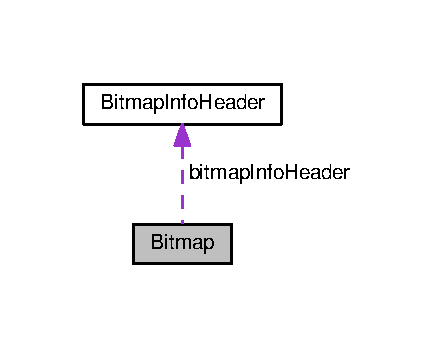
\includegraphics[width=209pt]{structBitmap__coll__graph}
\end{center}
\end{figure}
\subsection*{Public Attributes}
\begin{DoxyCompactItemize}
\item 
\hyperlink{structBitmapInfoHeader}{Bitmap\+Info\+Header} \hyperlink{structBitmap_a95c481a5ce1ff4af08cd135ca4af120b}{bitmap\+Info\+Header}
\item 
unsigned char $\ast$ \hyperlink{structBitmap_a581eac36ec50d730299b6df60e644750}{bitmap\+Data}
\end{DoxyCompactItemize}


\subsection{Detailed Description}
Represents a \hyperlink{structBitmap}{Bitmap}. 

\subsection{Member Data Documentation}
\index{Bitmap@{Bitmap}!bitmap\+Data@{bitmap\+Data}}
\index{bitmap\+Data@{bitmap\+Data}!Bitmap@{Bitmap}}
\subsubsection[{\texorpdfstring{bitmap\+Data}{bitmapData}}]{\setlength{\rightskip}{0pt plus 5cm}unsigned char$\ast$ Bitmap\+::bitmap\+Data}\hypertarget{structBitmap_a581eac36ec50d730299b6df60e644750}{}\label{structBitmap_a581eac36ec50d730299b6df60e644750}
\index{Bitmap@{Bitmap}!bitmap\+Info\+Header@{bitmap\+Info\+Header}}
\index{bitmap\+Info\+Header@{bitmap\+Info\+Header}!Bitmap@{Bitmap}}
\subsubsection[{\texorpdfstring{bitmap\+Info\+Header}{bitmapInfoHeader}}]{\setlength{\rightskip}{0pt plus 5cm}{\bf Bitmap\+Info\+Header} Bitmap\+::bitmap\+Info\+Header}\hypertarget{structBitmap_a95c481a5ce1ff4af08cd135ca4af120b}{}\label{structBitmap_a95c481a5ce1ff4af08cd135ca4af120b}


The documentation for this struct was generated from the following file\+:\begin{DoxyCompactItemize}
\item 
proj/src/\hyperlink{Bitmap_8h}{Bitmap.\+h}\end{DoxyCompactItemize}

\hypertarget{structBitmapFileHeader}{}\section{Bitmap\+File\+Header Struct Reference}
\label{structBitmapFileHeader}\index{Bitmap\+File\+Header@{Bitmap\+File\+Header}}


{\ttfamily \#include $<$Bitmap.\+h$>$}

\subsection*{Public Attributes}
\begin{DoxyCompactItemize}
\item 
unsigned short \hyperlink{structBitmapFileHeader_a139c2c2645bc00ddf4f5dc552872c1d1}{type}
\item 
unsigned int \hyperlink{structBitmapFileHeader_a0dcad71d9b17783c4d296c2c6d00ede0}{size}
\item 
unsigned int \hyperlink{structBitmapFileHeader_ab3833d77e2c28a216859a80ba8fac9f0}{reserved}
\item 
unsigned int \hyperlink{structBitmapFileHeader_a26ed598693b100ffd9e29c4dc77f3d92}{offset}
\end{DoxyCompactItemize}


\subsection{Member Data Documentation}
\index{Bitmap\+File\+Header@{Bitmap\+File\+Header}!offset@{offset}}
\index{offset@{offset}!Bitmap\+File\+Header@{Bitmap\+File\+Header}}
\subsubsection[{\texorpdfstring{offset}{offset}}]{\setlength{\rightskip}{0pt plus 5cm}unsigned int Bitmap\+File\+Header\+::offset}\hypertarget{structBitmapFileHeader_a26ed598693b100ffd9e29c4dc77f3d92}{}\label{structBitmapFileHeader_a26ed598693b100ffd9e29c4dc77f3d92}
\index{Bitmap\+File\+Header@{Bitmap\+File\+Header}!reserved@{reserved}}
\index{reserved@{reserved}!Bitmap\+File\+Header@{Bitmap\+File\+Header}}
\subsubsection[{\texorpdfstring{reserved}{reserved}}]{\setlength{\rightskip}{0pt plus 5cm}unsigned int Bitmap\+File\+Header\+::reserved}\hypertarget{structBitmapFileHeader_ab3833d77e2c28a216859a80ba8fac9f0}{}\label{structBitmapFileHeader_ab3833d77e2c28a216859a80ba8fac9f0}
\index{Bitmap\+File\+Header@{Bitmap\+File\+Header}!size@{size}}
\index{size@{size}!Bitmap\+File\+Header@{Bitmap\+File\+Header}}
\subsubsection[{\texorpdfstring{size}{size}}]{\setlength{\rightskip}{0pt plus 5cm}unsigned int Bitmap\+File\+Header\+::size}\hypertarget{structBitmapFileHeader_a0dcad71d9b17783c4d296c2c6d00ede0}{}\label{structBitmapFileHeader_a0dcad71d9b17783c4d296c2c6d00ede0}
\index{Bitmap\+File\+Header@{Bitmap\+File\+Header}!type@{type}}
\index{type@{type}!Bitmap\+File\+Header@{Bitmap\+File\+Header}}
\subsubsection[{\texorpdfstring{type}{type}}]{\setlength{\rightskip}{0pt plus 5cm}unsigned short Bitmap\+File\+Header\+::type}\hypertarget{structBitmapFileHeader_a139c2c2645bc00ddf4f5dc552872c1d1}{}\label{structBitmapFileHeader_a139c2c2645bc00ddf4f5dc552872c1d1}


The documentation for this struct was generated from the following file\+:\begin{DoxyCompactItemize}
\item 
proj/src/\hyperlink{Bitmap_8h}{Bitmap.\+h}\end{DoxyCompactItemize}

\hypertarget{structBitmapInfoHeader}{}\section{Bitmap\+Info\+Header Struct Reference}
\label{structBitmapInfoHeader}\index{Bitmap\+Info\+Header@{Bitmap\+Info\+Header}}


{\ttfamily \#include $<$Bitmap.\+h$>$}

\subsection*{Public Attributes}
\begin{DoxyCompactItemize}
\item 
unsigned int \hyperlink{structBitmapInfoHeader_a411fa70f6547a0360b33edcd3273d169}{size}
\item 
int \hyperlink{structBitmapInfoHeader_ac2034cfbada460819beed1ee24581c5d}{width}
\item 
int \hyperlink{structBitmapInfoHeader_aaa1d31efc13210020a38d435e4961df9}{height}
\item 
unsigned short \hyperlink{structBitmapInfoHeader_a9925e97e8bbc6b797afe2d22fbab45d6}{planes}
\item 
unsigned short \hyperlink{structBitmapInfoHeader_a1eebafc33573852f62a2e3d8adc25349}{bits}
\item 
unsigned int \hyperlink{structBitmapInfoHeader_a87fb38b0fe68db4bed899b9733d1b7e9}{compression}
\item 
unsigned int \hyperlink{structBitmapInfoHeader_a79bc984a7fd1c0f00ede6aa09143939f}{image\+Size}
\item 
int \hyperlink{structBitmapInfoHeader_a391cf1da75d16aee3b6539ccf5b29300}{x\+Resolution}
\item 
int \hyperlink{structBitmapInfoHeader_af2fadf9c216cc9f3ce401096e35be1b7}{y\+Resolution}
\item 
unsigned int \hyperlink{structBitmapInfoHeader_a4c543a08d1b72bdda2329b426a213e2a}{n\+Colors}
\item 
unsigned int \hyperlink{structBitmapInfoHeader_a9d87941fcc414085f7361fd89818ee3f}{important\+Colors}
\end{DoxyCompactItemize}


\subsection{Member Data Documentation}
\index{Bitmap\+Info\+Header@{Bitmap\+Info\+Header}!bits@{bits}}
\index{bits@{bits}!Bitmap\+Info\+Header@{Bitmap\+Info\+Header}}
\subsubsection[{\texorpdfstring{bits}{bits}}]{\setlength{\rightskip}{0pt plus 5cm}unsigned short Bitmap\+Info\+Header\+::bits}\hypertarget{structBitmapInfoHeader_a1eebafc33573852f62a2e3d8adc25349}{}\label{structBitmapInfoHeader_a1eebafc33573852f62a2e3d8adc25349}
\index{Bitmap\+Info\+Header@{Bitmap\+Info\+Header}!compression@{compression}}
\index{compression@{compression}!Bitmap\+Info\+Header@{Bitmap\+Info\+Header}}
\subsubsection[{\texorpdfstring{compression}{compression}}]{\setlength{\rightskip}{0pt plus 5cm}unsigned int Bitmap\+Info\+Header\+::compression}\hypertarget{structBitmapInfoHeader_a87fb38b0fe68db4bed899b9733d1b7e9}{}\label{structBitmapInfoHeader_a87fb38b0fe68db4bed899b9733d1b7e9}
\index{Bitmap\+Info\+Header@{Bitmap\+Info\+Header}!height@{height}}
\index{height@{height}!Bitmap\+Info\+Header@{Bitmap\+Info\+Header}}
\subsubsection[{\texorpdfstring{height}{height}}]{\setlength{\rightskip}{0pt plus 5cm}int Bitmap\+Info\+Header\+::height}\hypertarget{structBitmapInfoHeader_aaa1d31efc13210020a38d435e4961df9}{}\label{structBitmapInfoHeader_aaa1d31efc13210020a38d435e4961df9}
\index{Bitmap\+Info\+Header@{Bitmap\+Info\+Header}!image\+Size@{image\+Size}}
\index{image\+Size@{image\+Size}!Bitmap\+Info\+Header@{Bitmap\+Info\+Header}}
\subsubsection[{\texorpdfstring{image\+Size}{imageSize}}]{\setlength{\rightskip}{0pt plus 5cm}unsigned int Bitmap\+Info\+Header\+::image\+Size}\hypertarget{structBitmapInfoHeader_a79bc984a7fd1c0f00ede6aa09143939f}{}\label{structBitmapInfoHeader_a79bc984a7fd1c0f00ede6aa09143939f}
\index{Bitmap\+Info\+Header@{Bitmap\+Info\+Header}!important\+Colors@{important\+Colors}}
\index{important\+Colors@{important\+Colors}!Bitmap\+Info\+Header@{Bitmap\+Info\+Header}}
\subsubsection[{\texorpdfstring{important\+Colors}{importantColors}}]{\setlength{\rightskip}{0pt plus 5cm}unsigned int Bitmap\+Info\+Header\+::important\+Colors}\hypertarget{structBitmapInfoHeader_a9d87941fcc414085f7361fd89818ee3f}{}\label{structBitmapInfoHeader_a9d87941fcc414085f7361fd89818ee3f}
\index{Bitmap\+Info\+Header@{Bitmap\+Info\+Header}!n\+Colors@{n\+Colors}}
\index{n\+Colors@{n\+Colors}!Bitmap\+Info\+Header@{Bitmap\+Info\+Header}}
\subsubsection[{\texorpdfstring{n\+Colors}{nColors}}]{\setlength{\rightskip}{0pt plus 5cm}unsigned int Bitmap\+Info\+Header\+::n\+Colors}\hypertarget{structBitmapInfoHeader_a4c543a08d1b72bdda2329b426a213e2a}{}\label{structBitmapInfoHeader_a4c543a08d1b72bdda2329b426a213e2a}
\index{Bitmap\+Info\+Header@{Bitmap\+Info\+Header}!planes@{planes}}
\index{planes@{planes}!Bitmap\+Info\+Header@{Bitmap\+Info\+Header}}
\subsubsection[{\texorpdfstring{planes}{planes}}]{\setlength{\rightskip}{0pt plus 5cm}unsigned short Bitmap\+Info\+Header\+::planes}\hypertarget{structBitmapInfoHeader_a9925e97e8bbc6b797afe2d22fbab45d6}{}\label{structBitmapInfoHeader_a9925e97e8bbc6b797afe2d22fbab45d6}
\index{Bitmap\+Info\+Header@{Bitmap\+Info\+Header}!size@{size}}
\index{size@{size}!Bitmap\+Info\+Header@{Bitmap\+Info\+Header}}
\subsubsection[{\texorpdfstring{size}{size}}]{\setlength{\rightskip}{0pt plus 5cm}unsigned int Bitmap\+Info\+Header\+::size}\hypertarget{structBitmapInfoHeader_a411fa70f6547a0360b33edcd3273d169}{}\label{structBitmapInfoHeader_a411fa70f6547a0360b33edcd3273d169}
\index{Bitmap\+Info\+Header@{Bitmap\+Info\+Header}!width@{width}}
\index{width@{width}!Bitmap\+Info\+Header@{Bitmap\+Info\+Header}}
\subsubsection[{\texorpdfstring{width}{width}}]{\setlength{\rightskip}{0pt plus 5cm}int Bitmap\+Info\+Header\+::width}\hypertarget{structBitmapInfoHeader_ac2034cfbada460819beed1ee24581c5d}{}\label{structBitmapInfoHeader_ac2034cfbada460819beed1ee24581c5d}
\index{Bitmap\+Info\+Header@{Bitmap\+Info\+Header}!x\+Resolution@{x\+Resolution}}
\index{x\+Resolution@{x\+Resolution}!Bitmap\+Info\+Header@{Bitmap\+Info\+Header}}
\subsubsection[{\texorpdfstring{x\+Resolution}{xResolution}}]{\setlength{\rightskip}{0pt plus 5cm}int Bitmap\+Info\+Header\+::x\+Resolution}\hypertarget{structBitmapInfoHeader_a391cf1da75d16aee3b6539ccf5b29300}{}\label{structBitmapInfoHeader_a391cf1da75d16aee3b6539ccf5b29300}
\index{Bitmap\+Info\+Header@{Bitmap\+Info\+Header}!y\+Resolution@{y\+Resolution}}
\index{y\+Resolution@{y\+Resolution}!Bitmap\+Info\+Header@{Bitmap\+Info\+Header}}
\subsubsection[{\texorpdfstring{y\+Resolution}{yResolution}}]{\setlength{\rightskip}{0pt plus 5cm}int Bitmap\+Info\+Header\+::y\+Resolution}\hypertarget{structBitmapInfoHeader_af2fadf9c216cc9f3ce401096e35be1b7}{}\label{structBitmapInfoHeader_af2fadf9c216cc9f3ce401096e35be1b7}


The documentation for this struct was generated from the following file\+:\begin{DoxyCompactItemize}
\item 
proj/src/\hyperlink{Bitmap_8h}{Bitmap.\+h}\end{DoxyCompactItemize}

\hypertarget{structBitmaps__struct}{}\section{Bitmaps\+\_\+struct Struct Reference}
\label{structBitmaps__struct}\index{Bitmaps\+\_\+struct@{Bitmaps\+\_\+struct}}


{\ttfamily \#include $<$graphics.\+h$>$}



Collaboration diagram for Bitmaps\+\_\+struct\+:
\nopagebreak
\begin{figure}[H]
\begin{center}
\leavevmode
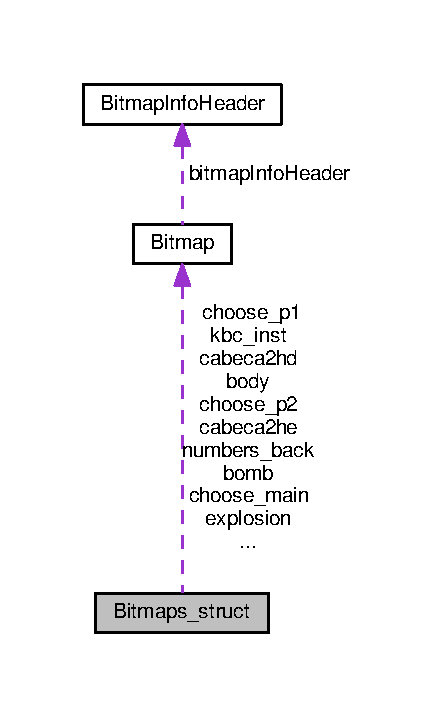
\includegraphics[width=209pt]{structBitmaps__struct__coll__graph}
\end{center}
\end{figure}
\subsection*{Public Attributes}
\begin{DoxyCompactItemize}
\item 
\hyperlink{structBitmap}{Bitmap} $\ast$ \hyperlink{group__graphics_ga90d36683bc99f1ee114191f6ae238990}{maca}
\begin{DoxyCompactList}\small\item\em fruit eaten by the snake to grow \end{DoxyCompactList}\item 
\hyperlink{structBitmap}{Bitmap} $\ast$ \hyperlink{group__graphics_gaa22a993c184e8cd76dbdf4830e5d108e}{body}
\begin{DoxyCompactList}\small\item\em body the s1 snake \end{DoxyCompactList}\item 
\hyperlink{structBitmap}{Bitmap} $\ast$ \hyperlink{group__graphics_ga8b84da2f75b89636fa34ff1cd47215f4}{body2}
\begin{DoxyCompactList}\small\item\em body of the s2 snake \end{DoxyCompactList}\item 
\hyperlink{structBitmap}{Bitmap} $\ast$ \hyperlink{group__graphics_ga0145b28638489d1308f15646be8042eb}{game\+\_\+over}
\item 
\hyperlink{structBitmap}{Bitmap} $\ast$ \hyperlink{group__graphics_ga2b3fa0b4fba818dec225a5cfa4ad2400}{bg}
\begin{DoxyCompactList}\small\item\em map used in SP and \hyperlink{structSnake}{Snake} and Mouse mode \end{DoxyCompactList}\item 
\hyperlink{structBitmap}{Bitmap} $\ast$ \hyperlink{group__graphics_gaca55c5a5f1494cb6d6c872d072b501d1}{bgmp}
\begin{DoxyCompactList}\small\item\em map used in the mode with 2 snakes \end{DoxyCompactList}\item 
\hyperlink{structBitmap}{Bitmap} $\ast$ \hyperlink{group__graphics_ga7740065d096144bd6f6f9457083584d9}{cabeca1hd}
\begin{DoxyCompactList}\small\item\em head of the s1 snake in the horizontal and positive directions \end{DoxyCompactList}\item 
\hyperlink{structBitmap}{Bitmap} $\ast$ \hyperlink{group__graphics_ga5989c4f83267088c9fdb6d1251d2e092}{cabeca1he}
\begin{DoxyCompactList}\small\item\em head of the s1 snake in the horizontal and negative directions \end{DoxyCompactList}\item 
\hyperlink{structBitmap}{Bitmap} $\ast$ \hyperlink{group__graphics_ga257cc4fca4ad7cceb125e4e43f62a17b}{cabeca1vc}
\begin{DoxyCompactList}\small\item\em head of the s1 snake in the vertical and negative directions \end{DoxyCompactList}\item 
\hyperlink{structBitmap}{Bitmap} $\ast$ \hyperlink{group__graphics_ga5737d3b582663eb60cd3fd47421707b3}{cabeca1vb}
\begin{DoxyCompactList}\small\item\em head of the s1 snake in the vertical and positive directions \end{DoxyCompactList}\item 
\hyperlink{structBitmap}{Bitmap} $\ast$ \hyperlink{group__graphics_ga74f59c6b2020b67b1e4c40b4d07b7dcb}{cabeca2hd}
\begin{DoxyCompactList}\small\item\em head of the s2 snake in the horizontal and positive directions \end{DoxyCompactList}\item 
\hyperlink{structBitmap}{Bitmap} $\ast$ \hyperlink{group__graphics_gad921a321d31f1c5f8430770b09949bd8}{cabeca2he}
\begin{DoxyCompactList}\small\item\em head of the s2 snake in the horizontal and negative directions \end{DoxyCompactList}\item 
\hyperlink{structBitmap}{Bitmap} $\ast$ \hyperlink{group__graphics_gabcbbaac60aafd8e9549fcef5fa6acb83}{cabeca2vc}
\begin{DoxyCompactList}\small\item\em head of the s2 snake in the vertical and negative directions \end{DoxyCompactList}\item 
\hyperlink{structBitmap}{Bitmap} $\ast$ \hyperlink{group__graphics_ga50f31017797fe46247d3ef644f6670c9}{cabeca2vb}
\begin{DoxyCompactList}\small\item\em head of the s2 snake in the vertical and positive directions \end{DoxyCompactList}\item 
\hyperlink{structBitmap}{Bitmap} $\ast$ \hyperlink{group__graphics_ga024eb6d4380a6df2938202e45547c241}{main\+\_\+menu}
\begin{DoxyCompactList}\small\item\em menu that appears at the start of the game \end{DoxyCompactList}\item 
\hyperlink{structBitmap}{Bitmap} $\ast$ \hyperlink{group__graphics_ga65a5f6d63fc1498c0bace1310dac202f}{mp\+\_\+menu}
\item 
\hyperlink{structBitmap}{Bitmap} $\ast$ \hyperlink{group__graphics_gaa9e2b675fd059f98d6fc79bff67f7918}{cursor}
\begin{DoxyCompactList}\small\item\em menu that appears when player selects multiplayer in main\+\_\+menu \end{DoxyCompactList}\item 
\hyperlink{structBitmap}{Bitmap} $\ast$ \hyperlink{group__graphics_ga055c85bff730277d284b6e00bb7d1b62}{numbers} \mbox{[}11\mbox{]}
\begin{DoxyCompactList}\small\item\em all the numbers from 0 to 9 in order,and the char \textquotesingle{}\+:\textquotesingle{} and \textquotesingle{}/\textquotesingle{} used in time and final scores \end{DoxyCompactList}\item 
\hyperlink{structBitmap}{Bitmap} $\ast$ \hyperlink{group__graphics_ga067f54df47f8ccad03f63d3b683f73a5}{sp\+\_\+inst}
\begin{DoxyCompactList}\small\item\em instructions of the singleplayer mode \end{DoxyCompactList}\item 
\hyperlink{structBitmap}{Bitmap} $\ast$ \hyperlink{group__graphics_ga4096188495e68d783bf3b8ac7871b7fa}{kbc\+\_\+inst}
\begin{DoxyCompactList}\small\item\em instructions of the snake gladiator mode \end{DoxyCompactList}\item 
\hyperlink{structBitmap}{Bitmap} $\ast$ \hyperlink{group__graphics_gaa403b7ac82d3c61224b7064f29790bd3}{mokb\+\_\+inst}
\begin{DoxyCompactList}\small\item\em instructions of the snake and mouse game mode \end{DoxyCompactList}\item 
\hyperlink{structBitmap}{Bitmap} $\ast$ \hyperlink{group__graphics_ga3b47ad4f61b00c3e5527f2bec90890b5}{pausesymb}
\begin{DoxyCompactList}\small\item\em pause message when the game is paused \end{DoxyCompactList}\item 
\hyperlink{structBitmap}{Bitmap} $\ast$ \hyperlink{group__graphics_ga86313247313ec7e1e264d13835d7d012}{bomb}
\begin{DoxyCompactList}\small\item\em bomb that might kill a snake \end{DoxyCompactList}\item 
\hyperlink{structBitmap}{Bitmap} $\ast$ \hyperlink{group__graphics_gac0df1ce2b02d6d52203766b8cb13c9bf}{explosion}
\begin{DoxyCompactList}\small\item\em explosion if snake collides with a bomb \end{DoxyCompactList}\item 
\hyperlink{structBitmap}{Bitmap} $\ast$ \hyperlink{group__graphics_gaf891e78c1cd9b89f53a3cf6032f88e71}{press\+\_\+enter}
\begin{DoxyCompactList}\small\item\em message press enter to continue at the end of each game \end{DoxyCompactList}\item 
\hyperlink{structBitmap}{Bitmap} $\ast$ \hyperlink{group__graphics_ga279ac50f42320cb39cbc02270e40597a}{player1}
\begin{DoxyCompactList}\small\item\em identifier of player 1 \end{DoxyCompactList}\item 
\hyperlink{structBitmap}{Bitmap} $\ast$ \hyperlink{group__graphics_gaaee24419ba914b7d473d1f5e06d84272}{player2}
\begin{DoxyCompactList}\small\item\em identifier of player 2 \end{DoxyCompactList}\item 
\hyperlink{structBitmap}{Bitmap} $\ast$ \hyperlink{group__graphics_ga500b120fd59215d5436fe2121557d34a}{small\+\_\+player1}
\item 
\hyperlink{structBitmap}{Bitmap} $\ast$ \hyperlink{group__graphics_ga6d0717c0730d1f4bf907299c4cb3fb97}{small\+\_\+player2}
\begin{DoxyCompactList}\small\item\em small identifier of player 1 \end{DoxyCompactList}\item 
\hyperlink{structBitmap}{Bitmap} $\ast$ \hyperlink{group__graphics_ga0fe961b9b328a12b933b0e3d2393e9d4}{choose\+\_\+main}
\begin{DoxyCompactList}\small\item\em menu to choose the body and the head of the it wants to use(only in modes with one snake) \end{DoxyCompactList}\item 
\hyperlink{structBitmap}{Bitmap} $\ast$ \hyperlink{group__graphics_ga1c051bf49f7de6f60eb93649684ebfb5}{choose\+\_\+p1}
\begin{DoxyCompactList}\small\item\em menu in 2 snakes mode, to choose the body of the snake of player1 (snake s1) \end{DoxyCompactList}\item 
\hyperlink{structBitmap}{Bitmap} $\ast$ \hyperlink{group__graphics_gabe0652c58a65bf0ccd93497ab08d9cfb}{choose\+\_\+p2}
\begin{DoxyCompactList}\small\item\em menu in 2 snakes mode, to choose the body of the snake of player2 (snake s2) \end{DoxyCompactList}\item 
\hyperlink{structBitmap}{Bitmap} $\ast$ \hyperlink{group__graphics_ga0d2f0b6ce3ed9e3fbdca9fb0e2197c8f}{counter1\+\_\+delay}
\begin{DoxyCompactList}\small\item\em number 1 in the countdown before the start of each game \end{DoxyCompactList}\item 
\hyperlink{structBitmap}{Bitmap} $\ast$ \hyperlink{group__graphics_gabbfd3197d8f58f68356e4c404c9b41a7}{counter2\+\_\+delay}
\begin{DoxyCompactList}\small\item\em number 2 in the count down before the start of each game \end{DoxyCompactList}\item 
\hyperlink{structBitmap}{Bitmap} $\ast$ \hyperlink{group__graphics_gac1063b5ae836e49a51d16a672c9cc11f}{counter3\+\_\+delay}
\begin{DoxyCompactList}\small\item\em number 3 in the count down before the start of each game \end{DoxyCompactList}\item 
\hyperlink{structBitmap}{Bitmap} $\ast$ \hyperlink{group__graphics_gac29eba55edb941d1896f1ea16ba40601}{numbers\+\_\+score} \mbox{[}10\mbox{]}
\begin{DoxyCompactList}\small\item\em numbers from 0 to 9 used to show the atual points of the snake ingame \end{DoxyCompactList}\item 
\hyperlink{structBitmap}{Bitmap} $\ast$ \hyperlink{group__graphics_ga416a4e7839cf0a547fcf830f0e5e3cf3}{numbers\+\_\+back}
\begin{DoxyCompactList}\small\item\em simple black background to put the numbers stated above, and to make a standard new wall that the snakes should\textquotesingle{}nt collide with \end{DoxyCompactList}\end{DoxyCompactItemize}


\subsection{Detailed Description}
all bitmaps used in the game 

The documentation for this struct was generated from the following file\+:\begin{DoxyCompactItemize}
\item 
proj/src/\hyperlink{graphics_8h}{graphics.\+h}\end{DoxyCompactItemize}

\hypertarget{structdate__rtc}{}\section{date\+\_\+rtc Struct Reference}
\label{structdate__rtc}\index{date\+\_\+rtc@{date\+\_\+rtc}}


{\ttfamily \#include $<$date.\+h$>$}

\subsection*{Public Attributes}
\begin{DoxyCompactItemize}
\item 
unsigned long \hyperlink{structdate__rtc_a4a231dccac478c1e2eb419ee34535e0e}{hour}
\begin{DoxyCompactList}\small\item\em the hour \end{DoxyCompactList}\item 
unsigned long \hyperlink{structdate__rtc_a6ea5d53162f2139e1e2a8d59bd3083b9}{min}
\begin{DoxyCompactList}\small\item\em the minutes \end{DoxyCompactList}\item 
unsigned long \hyperlink{structdate__rtc_a4d0f917003e201fbfe662d4c91907645}{sec}
\begin{DoxyCompactList}\small\item\em the seconds \end{DoxyCompactList}\item 
unsigned long \hyperlink{structdate__rtc_aafb65ff718f63c0e56aff1168ab3c154}{day}
\begin{DoxyCompactList}\small\item\em the day of the year \end{DoxyCompactList}\item 
unsigned long \hyperlink{structdate__rtc_a12309edd1455518380682d3241cd4b75}{month}
\begin{DoxyCompactList}\small\item\em the month of the year \end{DoxyCompactList}\item 
unsigned long \hyperlink{structdate__rtc_abf8b053026cf0db4cc2d260ce9cce925}{year}
\begin{DoxyCompactList}\small\item\em the year \end{DoxyCompactList}\end{DoxyCompactItemize}


\subsection{Detailed Description}
Stored time values of the rtc 

\subsection{Member Data Documentation}
\index{date\+\_\+rtc@{date\+\_\+rtc}!day@{day}}
\index{day@{day}!date\+\_\+rtc@{date\+\_\+rtc}}
\subsubsection[{\texorpdfstring{day}{day}}]{\setlength{\rightskip}{0pt plus 5cm}unsigned long date\+\_\+rtc\+::day}\hypertarget{structdate__rtc_aafb65ff718f63c0e56aff1168ab3c154}{}\label{structdate__rtc_aafb65ff718f63c0e56aff1168ab3c154}


the day of the year 

\index{date\+\_\+rtc@{date\+\_\+rtc}!hour@{hour}}
\index{hour@{hour}!date\+\_\+rtc@{date\+\_\+rtc}}
\subsubsection[{\texorpdfstring{hour}{hour}}]{\setlength{\rightskip}{0pt plus 5cm}unsigned long date\+\_\+rtc\+::hour}\hypertarget{structdate__rtc_a4a231dccac478c1e2eb419ee34535e0e}{}\label{structdate__rtc_a4a231dccac478c1e2eb419ee34535e0e}


the hour 

\index{date\+\_\+rtc@{date\+\_\+rtc}!min@{min}}
\index{min@{min}!date\+\_\+rtc@{date\+\_\+rtc}}
\subsubsection[{\texorpdfstring{min}{min}}]{\setlength{\rightskip}{0pt plus 5cm}unsigned long date\+\_\+rtc\+::min}\hypertarget{structdate__rtc_a6ea5d53162f2139e1e2a8d59bd3083b9}{}\label{structdate__rtc_a6ea5d53162f2139e1e2a8d59bd3083b9}


the minutes 

\index{date\+\_\+rtc@{date\+\_\+rtc}!month@{month}}
\index{month@{month}!date\+\_\+rtc@{date\+\_\+rtc}}
\subsubsection[{\texorpdfstring{month}{month}}]{\setlength{\rightskip}{0pt plus 5cm}unsigned long date\+\_\+rtc\+::month}\hypertarget{structdate__rtc_a12309edd1455518380682d3241cd4b75}{}\label{structdate__rtc_a12309edd1455518380682d3241cd4b75}


the month of the year 

\index{date\+\_\+rtc@{date\+\_\+rtc}!sec@{sec}}
\index{sec@{sec}!date\+\_\+rtc@{date\+\_\+rtc}}
\subsubsection[{\texorpdfstring{sec}{sec}}]{\setlength{\rightskip}{0pt plus 5cm}unsigned long date\+\_\+rtc\+::sec}\hypertarget{structdate__rtc_a4d0f917003e201fbfe662d4c91907645}{}\label{structdate__rtc_a4d0f917003e201fbfe662d4c91907645}


the seconds 

\index{date\+\_\+rtc@{date\+\_\+rtc}!year@{year}}
\index{year@{year}!date\+\_\+rtc@{date\+\_\+rtc}}
\subsubsection[{\texorpdfstring{year}{year}}]{\setlength{\rightskip}{0pt plus 5cm}unsigned long date\+\_\+rtc\+::year}\hypertarget{structdate__rtc_abf8b053026cf0db4cc2d260ce9cce925}{}\label{structdate__rtc_abf8b053026cf0db4cc2d260ce9cce925}


the year 



The documentation for this struct was generated from the following file\+:\begin{DoxyCompactItemize}
\item 
\hyperlink{date_8h}{date.\+h}\end{DoxyCompactItemize}

\hypertarget{structGame__object}{}\section{Game\+\_\+object Struct Reference}
\label{structGame__object}\index{Game\+\_\+object@{Game\+\_\+object}}


{\ttfamily \#include $<$objects.\+h$>$}

\subsection*{Public Attributes}
\begin{DoxyCompactItemize}
\item 
unsigned short \hyperlink{group__object_ga41a0b70059db5a8364cb00caed5f7860}{row}
\item 
unsigned short \hyperlink{group__object_ga26747c58af9aac0a386f3be5b5302d23}{col}
\begin{DoxyCompactList}\small\item\em position in the matrix\+\_\+graphics \end{DoxyCompactList}\item 
int \hyperlink{group__object_gaa3e8af9c364161ddf47359bba651e9cf}{point\+\_\+value}
\item 
\hyperlink{group__object_ga90ab20efa1890ce46e743d7569ce7cec}{object\+\_\+name} \hyperlink{group__object_ga27d8ddc2e36ab28af25f9698f1b11e49}{name}
\begin{DoxyCompactList}\small\item\em how many points the object is valued (U\+N\+U\+S\+ED) \end{DoxyCompactList}\end{DoxyCompactItemize}


\subsection{Detailed Description}
Objects used in game 

The documentation for this struct was generated from the following file\+:\begin{DoxyCompactItemize}
\item 
\hyperlink{objects_8h}{objects.\+h}\end{DoxyCompactItemize}

\hypertarget{structmmap__t}{}\section{mmap\+\_\+t Struct Reference}
\label{structmmap__t}\index{mmap\+\_\+t@{mmap\+\_\+t}}


{\ttfamily \#include $<$lmlib.\+h$>$}

\subsection*{Public Attributes}
\begin{DoxyCompactItemize}
\item 
phys\+\_\+bytes \hyperlink{group__lmlib_gaa6ac1ee0e0fadea4a4f85b48c8359ae4}{phys}
\begin{DoxyCompactList}\small\item\em physical address \end{DoxyCompactList}\item 
void $\ast$ \hyperlink{group__lmlib_ga4de93144fb3ffbceb9bd1f3009d6d98c}{virtual}
\begin{DoxyCompactList}\small\item\em virtual address \end{DoxyCompactList}\item 
unsigned long \hyperlink{group__lmlib_gaf1cdc5384a402fddf33f400a5e1e5e45}{size}
\begin{DoxyCompactList}\small\item\em size of memory region \end{DoxyCompactList}\end{DoxyCompactItemize}


\subsection{Detailed Description}
Struct that keeps info regarding the mapping of physical memory to virtual memory 

The documentation for this struct was generated from the following file\+:\begin{DoxyCompactItemize}
\item 
\hyperlink{lmlib_8h}{lmlib.\+h}\end{DoxyCompactItemize}

\hypertarget{structSegment}{}\section{Segment Struct Reference}
\label{structSegment}\index{Segment@{Segment}}


{\ttfamily \#include $<$snake.\+h$>$}



Collaboration diagram for Segment\+:
\nopagebreak
\begin{figure}[H]
\begin{center}
\leavevmode
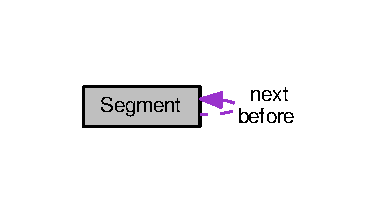
\includegraphics[width=182pt]{structSegment__coll__graph}
\end{center}
\end{figure}
\subsection*{Public Attributes}
\begin{DoxyCompactItemize}
\item 
unsigned short \hyperlink{group__snake_ga5c86edfec316ae4d5033a85525babed6}{row}
\item 
unsigned short \hyperlink{group__snake_ga3369387554e0ec37bb04c153c3529ed9}{col}
\begin{DoxyCompactList}\small\item\em position in the matrix\+\_\+graphics \end{DoxyCompactList}\item 
unsigned short \hyperlink{group__snake_gacf610091b7f59fb0f1f37c6df4e14c18}{direction}
\begin{DoxyCompactList}\small\item\em direction it is facing, vertical or horizontal \end{DoxyCompactList}\item 
unsigned short \hyperlink{group__snake_gadd6c62d3fd2c3aab9175c07694fdc075}{orientation}
\item 
struct \hyperlink{structSegment}{Segment} $\ast$ \hyperlink{group__snake_ga20fb1741f720a656ec35972c2305a2d9}{next}
\begin{DoxyCompactList}\small\item\em orientation it is facing. if its moving in positive direction or negative \end{DoxyCompactList}\item 
struct \hyperlink{structSegment}{Segment} $\ast$ \hyperlink{group__snake_ga60c4d032ff0baffc3c99c1630dae24e3}{before}
\begin{DoxyCompactList}\small\item\em pointer to the next body part(like a linked list) \end{DoxyCompactList}\end{DoxyCompactItemize}


\subsection{Detailed Description}
\hyperlink{structSnake}{Snake} using a linked list 

The documentation for this struct was generated from the following file\+:\begin{DoxyCompactItemize}
\item 
\hyperlink{snake_8h}{snake.\+h}\end{DoxyCompactItemize}

\hypertarget{structSnake}{}\section{Snake Struct Reference}
\label{structSnake}\index{Snake@{Snake}}


Represents a \hyperlink{structSnake}{Snake}.  




{\ttfamily \#include $<$snake.\+h$>$}



Collaboration diagram for Snake\+:
\nopagebreak
\begin{figure}[H]
\begin{center}
\leavevmode
\includegraphics[width=182pt]{structSnake__coll__graph}
\end{center}
\end{figure}
\subsection*{Public Attributes}
\begin{DoxyCompactItemize}
\item 
\hyperlink{group__snake_ga40f634d31a1f9372bd182d65da207a21}{segment\+\_\+snake} $\ast$ \hyperlink{group__snake_gaf63e50ac65f365d67ae3975a178cba8c}{head}
\begin{DoxyCompactList}\small\item\em pointer to the head of the snake \end{DoxyCompactList}\item 
\hyperlink{group__snake_ga40f634d31a1f9372bd182d65da207a21}{segment\+\_\+snake} $\ast$ \hyperlink{group__snake_gada92e10f60af5b1afdb7318df07a1a33}{tail}
\item 
unsigned int \hyperlink{group__snake_ga29ba822024f7651a9fa0c80df840252b}{size}
\begin{DoxyCompactList}\small\item\em pointer to the tail of the snake \end{DoxyCompactList}\item 
unsigned short \hyperlink{group__snake_gac444a5a9306233f5be0b603335785b3d}{velocity}
\begin{DoxyCompactList}\small\item\em size of the snake(number of segment\+\_\+snake) \end{DoxyCompactList}\item 
unsigned short \hyperlink{group__snake_ga7339bbc2027ffeb1ce00f24a834610cc}{boost}
\begin{DoxyCompactList}\small\item\em velocity the snake is moving \end{DoxyCompactList}\item 
unsigned short \hyperlink{group__snake_ga0b46bc6b402fd8999c6998eca1806c3e}{boost\+\_\+time}
\begin{DoxyCompactList}\small\item\em flag to know if the snake is boosting \end{DoxyCompactList}\end{DoxyCompactItemize}


\subsection{Detailed Description}
Represents a \hyperlink{structSnake}{Snake}. 

The documentation for this struct was generated from the following file\+:\begin{DoxyCompactItemize}
\item 
proj/src/\hyperlink{snake_8h}{snake.\+h}\end{DoxyCompactItemize}

\chapter{File Documentation}
\hypertarget{assem__scan_8d}{}\section{proj/src/assem\+\_\+scan.d File Reference}
\label{assem__scan_8d}\index{proj/src/assem\+\_\+scan.\+d@{proj/src/assem\+\_\+scan.\+d}}

\hypertarget{Bitmap_8c}{}\section{Bitmap.\+c File Reference}
\label{Bitmap_8c}\index{Bitmap.\+c@{Bitmap.\+c}}
{\ttfamily \#include \char`\"{}Bitmap.\+h\char`\"{}}\\*
{\ttfamily \#include \char`\"{}stdio.\+h\char`\"{}}\\*
{\ttfamily \#include \char`\"{}constants.\+h\char`\"{}}\\*
Include dependency graph for Bitmap.\+c\+:
\nopagebreak
\begin{figure}[H]
\begin{center}
\leavevmode
\includegraphics[width=289pt]{Bitmap_8c__incl}
\end{center}
\end{figure}
\subsection*{Functions}
\begin{DoxyCompactItemize}
\item 
\hyperlink{structBitmap}{Bitmap} $\ast$ \hyperlink{group__Bitmap_ga3506880ffd407c36eb8aaddd2c1606d2}{load\+Bitmap} (const char $\ast$filename)
\begin{DoxyCompactList}\small\item\em Loads a bmp image. \end{DoxyCompactList}\item 
void \hyperlink{group__Bitmap_ga18d05a1c671f4638bc63d37874efb9d4}{draw\+Bitmap} (\hyperlink{structBitmap}{Bitmap} $\ast$\hyperlink{menu_8c_a9ac459dc630a69c0162412290c4cc1f6}{bmp}, int x, int y, \hyperlink{group__Bitmap_gacdfaca60ec19c0265bac2692d7982726}{Alignment} alignment)
\begin{DoxyCompactList}\small\item\em Draws an unscaled, unrotated bitmap at the given position, and verify each pixel to know if it is a transparent pixel (color rgb(255, 0, 255) ) \end{DoxyCompactList}\item 
void \hyperlink{group__Bitmap_ga362eae5066441f6797d2289c5ccd493d}{drawbackground} (\hyperlink{structBitmap}{Bitmap} $\ast$\hyperlink{menu_8c_a9ac459dc630a69c0162412290c4cc1f6}{bmp}, int x, int y, \hyperlink{group__Bitmap_gacdfaca60ec19c0265bac2692d7982726}{Alignment} alignment)
\begin{DoxyCompactList}\small\item\em Draws an unscaled, unrotated bitmap at the given position. \end{DoxyCompactList}\item 
void \hyperlink{group__Bitmap_ga08c1d4f4fff81df260d979ea8fc1aa61}{delete\+Bitmap} (\hyperlink{structBitmap}{Bitmap} $\ast$\hyperlink{menu_8c_a9ac459dc630a69c0162412290c4cc1f6}{bmp})
\begin{DoxyCompactList}\small\item\em Destroys the given bitmap, freeing all resources used by it. \end{DoxyCompactList}\end{DoxyCompactItemize}

\hypertarget{Bitmap_8d}{}\section{Bitmap.\+d File Reference}
\label{Bitmap_8d}\index{Bitmap.\+d@{Bitmap.\+d}}

\hypertarget{Bitmap_8h}{}\section{proj/src/\+Bitmap.h File Reference}
\label{Bitmap_8h}\index{proj/src/\+Bitmap.\+h@{proj/src/\+Bitmap.\+h}}
{\ttfamily \#include \char`\"{}video\+\_\+gr.\+h\char`\"{}}\\*
Include dependency graph for Bitmap.\+h\+:
\nopagebreak
\begin{figure}[H]
\begin{center}
\leavevmode
\includegraphics[width=171pt]{Bitmap_8h__incl}
\end{center}
\end{figure}
This graph shows which files directly or indirectly include this file\+:
\nopagebreak
\begin{figure}[H]
\begin{center}
\leavevmode
\includegraphics[width=350pt]{Bitmap_8h__dep__incl}
\end{center}
\end{figure}
\subsection*{Classes}
\begin{DoxyCompactItemize}
\item 
struct \hyperlink{structBitmapFileHeader}{Bitmap\+File\+Header}
\item 
struct \hyperlink{structBitmapInfoHeader}{Bitmap\+Info\+Header}
\item 
struct \hyperlink{structBitmap}{Bitmap}
\begin{DoxyCompactList}\small\item\em Represents a \hyperlink{structBitmap}{Bitmap}. \end{DoxyCompactList}\end{DoxyCompactItemize}
\subsection*{Enumerations}
\begin{DoxyCompactItemize}
\item 
enum \hyperlink{group__Bitmap_gacdfaca60ec19c0265bac2692d7982726}{Alignment} \{ \hyperlink{group__Bitmap_ggacdfaca60ec19c0265bac2692d7982726a6ec599857e15466988726932dd592305}{A\+L\+I\+G\+N\+\_\+\+L\+E\+FT}, 
\hyperlink{group__Bitmap_ggacdfaca60ec19c0265bac2692d7982726a5624165187e56db612253e608a45b1c6}{A\+L\+I\+G\+N\+\_\+\+C\+E\+N\+T\+ER}, 
\hyperlink{group__Bitmap_ggacdfaca60ec19c0265bac2692d7982726a9c81840e8cad46418b39a8b74a246354}{A\+L\+I\+G\+N\+\_\+\+R\+I\+G\+HT}
 \}
\end{DoxyCompactItemize}
\subsection*{Functions}
\begin{DoxyCompactItemize}
\item 
\hyperlink{structBitmap}{Bitmap} $\ast$ \hyperlink{group__Bitmap_ga3506880ffd407c36eb8aaddd2c1606d2}{load\+Bitmap} (const char $\ast$filename)
\begin{DoxyCompactList}\small\item\em Loads a bmp image. \end{DoxyCompactList}\item 
void \hyperlink{group__Bitmap_ga18d05a1c671f4638bc63d37874efb9d4}{draw\+Bitmap} (\hyperlink{structBitmap}{Bitmap} $\ast$bitmap, int x, int y, \hyperlink{group__Bitmap_gacdfaca60ec19c0265bac2692d7982726}{Alignment} alignment)
\begin{DoxyCompactList}\small\item\em Draws an unscaled, unrotated bitmap at the given position, and verify each pixel to know if it is a transparent pixel (color rgb(255, 0, 255) ) \end{DoxyCompactList}\item 
void \hyperlink{group__Bitmap_ga362eae5066441f6797d2289c5ccd493d}{drawbackground} (\hyperlink{structBitmap}{Bitmap} $\ast$\hyperlink{menu_8c_a9ac459dc630a69c0162412290c4cc1f6}{bmp}, int x, int y, \hyperlink{group__Bitmap_gacdfaca60ec19c0265bac2692d7982726}{Alignment} alignment)
\begin{DoxyCompactList}\small\item\em Draws an unscaled, unrotated bitmap at the given position. \end{DoxyCompactList}\item 
void \hyperlink{group__Bitmap_ga08c1d4f4fff81df260d979ea8fc1aa61}{delete\+Bitmap} (\hyperlink{structBitmap}{Bitmap} $\ast$\hyperlink{menu_8c_a9ac459dc630a69c0162412290c4cc1f6}{bmp})
\begin{DoxyCompactList}\small\item\em Destroys the given bitmap, freeing all resources used by it. \end{DoxyCompactList}\end{DoxyCompactItemize}
\subsection*{Variables}
\begin{DoxyCompactItemize}
\item 
static unsigned \hyperlink{group__Bitmap_ga43e7e5a0a8f9069e6413b2066ca52f3e}{h\+\_\+res}
\item 
static unsigned \hyperlink{group__Bitmap_ga5bda1b499253a8fbf3cab646f8760391}{v\+\_\+res}
\item 
static unsigned \hyperlink{group__Bitmap_ga89fa3fb58e975d148fcb2413e24b78a1}{bits\+\_\+per\+\_\+pixel}
\item 
static unsigned \hyperlink{group__Bitmap_ga59559f1bdfa71061d06d9ea27c0748ed}{screen\+\_\+size}
\end{DoxyCompactItemize}

\hypertarget{constants_8h}{}\section{constants.\+h File Reference}
\label{constants_8h}\index{constants.\+h@{constants.\+h}}
{\ttfamily \#include \char`\"{}i8254.\+h\char`\"{}}\\*
Include dependency graph for constants.\+h\+:
\nopagebreak
\begin{figure}[H]
\begin{center}
\leavevmode
\includegraphics[width=148pt]{constants_8h__incl}
\end{center}
\end{figure}
This graph shows which files directly or indirectly include this file\+:
\nopagebreak
\begin{figure}[H]
\begin{center}
\leavevmode
\includegraphics[width=350pt]{constants_8h__dep__incl}
\end{center}
\end{figure}
\subsection*{Macros}
\begin{DoxyCompactItemize}
\item 
\#define \hyperlink{constants_8h_aa6cb9ba4125464b6bc39f76b279b3e45}{H\+O\+R\+I\+Z\+O\+N\+T\+A\+L\+\_\+\+P\+A\+I\+NT}~0
\item 
\#define \hyperlink{constants_8h_a865a372b01ab32389c815c67f25b14be}{V\+E\+R\+T\+I\+C\+A\+L\+\_\+\+P\+A\+I\+NT}~1
\item 
\#define \hyperlink{constants_8h_ae36fc325bc821e866e90d0e66f9cc168}{K\+B\+\_\+\+I\+RQ}~1
\item 
\#define \hyperlink{constants_8h_a1f7e79cfe81dc06414550fa52418941e}{S\+T\+A\+T\+U\+S\+\_\+\+R\+EG}~0x64
\item 
\#define \hyperlink{constants_8h_aeff3162e464a9081f73e3765f199d7c1}{K\+B\+D\+\_\+\+O\+U\+T\+\_\+\+B\+UF}~0x60
\item 
\#define \hyperlink{constants_8h_a45967c9e25447ba853cf6fb4ac545fe6}{O\+BF}~\hyperlink{group__i8254_ga3a8ea58898cb58fc96013383d39f482c}{B\+IT}(0)
\item 
\#define \hyperlink{constants_8h_a3c48b10907056351582baf9f6478598e}{I\+BF}~\hyperlink{group__i8254_ga3a8ea58898cb58fc96013383d39f482c}{B\+IT}(1)
\item 
\#define \hyperlink{constants_8h_a8c83f07c11b3fae6015d16164257e253}{E\+S\+C\+\_\+\+C\+O\+DE}~0x81
\item 
\#define \hyperlink{constants_8h_ad315ce436b88e78c266532e4714dd197}{U\+P\+\_\+\+A\+R\+R\+OW}~0x\+E048
\item 
\#define \hyperlink{constants_8h_a5b1eca6358420b8748a151949d3119fa}{D\+O\+W\+N\+\_\+\+A\+R\+R\+OW}~0x\+E050
\item 
\#define \hyperlink{constants_8h_ae78ccf44cb7970752cbfeb22e6a66d14}{L\+E\+F\+T\+\_\+\+A\+R\+R\+OW}~0x\+E04B
\item 
\#define \hyperlink{constants_8h_a9ed2533108b634266a6261c8f37e4fc0}{R\+I\+G\+H\+T\+\_\+\+A\+R\+R\+OW}~0x\+E04D
\item 
\#define \hyperlink{constants_8h_a2e092124f706e9898a26f3d0c6dd33d3}{A\+\_\+\+K\+EY}~0x9E
\item 
\#define \hyperlink{constants_8h_a8cb726577cd35fc0582744b2270e192f}{W\+\_\+\+K\+EY}~0x91
\item 
\#define \hyperlink{constants_8h_a38916d959d471a2781d390910271b6b5}{S\+\_\+\+K\+EY}~0x9F
\item 
\#define \hyperlink{constants_8h_a23c8dc1c6696b91ba6b96f2dca53b7ba}{D\+\_\+\+K\+EY}~0x\+A0
\item 
\#define \hyperlink{constants_8h_af4bced5cf8ed55746d4b5d34f9a0fe39}{E\+N\+T\+ER}~0x001C
\item 
\#define \hyperlink{constants_8h_ac104deaeab94d33941c04e9e6940ee05}{C\+T\+R\+L\+\_\+\+M\+A\+KE}~0x1D
\item 
\#define \hyperlink{constants_8h_a9231077dba7026f0084bd7e55fad858c}{C\+T\+R\+L\+\_\+\+B\+R\+E\+AK}~0x9D
\item 
\#define \hyperlink{constants_8h_aa15f30055cded11b1e05310e83369105}{S\+H\+I\+F\+T\+\_\+\+M\+A\+KE}~0x36
\item 
\#define \hyperlink{constants_8h_a67b637e5b9b75a151db0bfc05d9de583}{S\+H\+I\+F\+T\+\_\+\+B\+R\+E\+AK}~0x\+B6
\item 
\#define \hyperlink{constants_8h_a7ee721f08221a8768d7af86476d02a38}{N\+B\+IT}(n)~(0x\+F\+F$^\wedge$\+B\+I\+T(n))
\item 
\#define \hyperlink{constants_8h_aec543895ecec3c62da6cfa35c035c000}{O\+U\+T\+\_\+\+B\+U\+F\+\_\+2\+B\+Y\+T\+ES}~0x\+E0
\item 
\#define \hyperlink{constants_8h_a1a522aa19bcb695a9df30032a893bee3}{D\+E\+L\+A\+Y\+\_\+\+US}~20000
\item 
\#define \hyperlink{constants_8h_a307ab71673e26ec42b28a3bca05d4cb5}{P\+A\+R\+\_\+\+E\+RR}~\hyperlink{group__i8254_ga3a8ea58898cb58fc96013383d39f482c}{B\+IT}(7)
\item 
\#define \hyperlink{constants_8h_ad16f61e2bf70f6c7685e826224ed177f}{T\+O\+\_\+\+E\+RR}~\hyperlink{group__i8254_ga3a8ea58898cb58fc96013383d39f482c}{B\+IT}(6)
\item 
\#define \hyperlink{constants_8h_adf1b9da7c6d6c0d06446232d959f173d}{O\+N\+\_\+\+O\+F\+F\+\_\+\+L\+E\+DS}~0x\+ED
\item 
\#define \hyperlink{constants_8h_a6d57c7927a10f638c83046b52c8caac9}{K\+B\+C\+\_\+\+C\+M\+D\+\_\+\+R\+EG}~0x64
\item 
\#define \hyperlink{constants_8h_a6f6489887e08bff4887d0bc5dcf214d8}{A\+CK}~0x\+FA
\item 
\#define \hyperlink{constants_8h_a92f67631ef5a97e4a266c15bc710776d}{R\+E\+S\+E\+ND}~0x\+FE
\item 
\#define \hyperlink{constants_8h_a8fe83ac76edc595f6b98cd4a4127aed5}{E\+R\+R\+OR}~0x\+FC
\item 
\#define \hyperlink{constants_8h_ab851a6d21990062b102fbbbe27bab3ed}{M\+S\+\_\+\+O\+U\+T\+\_\+\+B\+UF}~0x60
\item 
\#define \hyperlink{constants_8h_a2662b4549668697ef89b7f335e9214e2}{M\+S\+\_\+\+I\+RQ}~12
\item 
\#define \hyperlink{constants_8h_a1b41fd2be63532d4ab910f8b256c3811}{A\+UX}~\hyperlink{group__i8254_ga3a8ea58898cb58fc96013383d39f482c}{B\+IT}(5)
\item 
\#define \hyperlink{constants_8h_aeaa6eccac0c5817874f172bae2a4bc77}{W\+R\+I\+T\+E\+\_\+\+B\+\_\+\+M\+O\+U\+SE}~0x\+D4
\item 
\#define \hyperlink{constants_8h_ab3919f33b46e0808c4ed1c56a6a423f2}{S\+T\+R\+E\+A\+M\+\_\+\+M\+O\+DE}~0x\+EA
\item 
\#define \hyperlink{constants_8h_aff3f5b3c04a3dfac99ae8967e5b4fadb}{D\+I\+S\+A\+B\+L\+E\+\_\+\+S\+T\+R\+E\+AM}~0x\+F5
\item 
\#define \hyperlink{constants_8h_a57b2d84fe9fb15bee8b83e8d52e785aa}{E\+N\+A\+B\+L\+E\+\_\+\+S\+T\+R\+E\+AM}~0x\+F4
\item 
\#define \hyperlink{constants_8h_a958518a45b12053ae33606ee7cb68a55}{N\+A\+CK}~0x\+FE
\item 
\#define \hyperlink{constants_8h_ab74d8cf9ec50650fee5058cb33a9160e}{S\+T\+A\+T\+U\+S\+\_\+\+R\+E\+Q\+U\+E\+ST}~0x\+E9
\item 
\#define \hyperlink{constants_8h_af01c30c610c2b5244d7146fddd9781fc}{C\+O\+N\+F\+\_\+\+B\+Y\+T\+E2\+\_\+\+Z\+E\+R\+OS}~\hyperlink{group__i8254_ga3a8ea58898cb58fc96013383d39f482c}{B\+IT}(7) \& \hyperlink{group__i8254_ga3a8ea58898cb58fc96013383d39f482c}{B\+IT}(6) \& \hyperlink{group__i8254_ga3a8ea58898cb58fc96013383d39f482c}{B\+IT}(5) \& \hyperlink{group__i8254_ga3a8ea58898cb58fc96013383d39f482c}{B\+IT}(4) \& \hyperlink{group__i8254_ga3a8ea58898cb58fc96013383d39f482c}{B\+IT}(3) \& \hyperlink{group__i8254_ga3a8ea58898cb58fc96013383d39f482c}{B\+IT}(2)
\item 
\#define \hyperlink{constants_8h_a356ebf158dd5c7f57a9edca8e995316f}{R\+E\+A\+D\+\_\+\+K\+BC}~0x20
\item 
\#define \hyperlink{constants_8h_ac7729e77be00851ee7c8e066bd034bf8}{V\+E\+R\+I\+F\+Y\+\_\+\+P\+A\+C\+K\+ET}~\hyperlink{group__i8254_ga3a8ea58898cb58fc96013383d39f482c}{B\+IT}(3)
\item 
\#define \hyperlink{constants_8h_a2cf88c3fc2bda8c5155ef3053f85957c}{V\+E\+R\+I\+F\+Y\+\_\+\+E\+M\+P\+T\+Y\+\_\+\+B\+UF}~\hyperlink{group__i8254_ga3a8ea58898cb58fc96013383d39f482c}{B\+IT}(5)
\item 
\#define \hyperlink{constants_8h_a058d3742e87fd0ea1b8d620ec95e88d9}{C\+O\+N\+F\+\_\+\+F\+I\+R\+S\+T\+\_\+\+B\+Y\+TE}~\hyperlink{group__i8254_ga3a8ea58898cb58fc96013383d39f482c}{B\+IT}(7) \& \hyperlink{group__i8254_ga3a8ea58898cb58fc96013383d39f482c}{B\+IT}(3)
\item 
\#define \hyperlink{constants_8h_aeb17351958162535ab6af2cd6b030955}{R\+I\+G\+H\+T\+\_\+\+B\+U\+T\+T\+ON}~\hyperlink{group__i8254_ga3a8ea58898cb58fc96013383d39f482c}{B\+IT}(1)
\item 
\#define \hyperlink{constants_8h_aea4935ff922fa4fbbc0f03fc250e268b}{M\+I\+D\+D\+L\+E\+\_\+\+B\+U\+T\+T\+ON}~\hyperlink{group__i8254_ga3a8ea58898cb58fc96013383d39f482c}{B\+IT}(2)
\item 
\#define \hyperlink{constants_8h_abbc8382ae4ea521f03c119a14478b759}{L\+E\+F\+T\+\_\+\+B\+U\+T\+T\+ON}~\hyperlink{group__i8254_ga3a8ea58898cb58fc96013383d39f482c}{B\+IT}(0)
\item 
\#define \hyperlink{constants_8h_a10ff10afd2a3179ae42e67a12fd8d7fd}{S\+C\+A\+L\+I\+NG}~\hyperlink{group__i8254_ga3a8ea58898cb58fc96013383d39f482c}{B\+IT}(4)
\item 
\#define \hyperlink{constants_8h_a782efbd04012530bb88bd5660dc24af6}{D\+A\+T\+A\+\_\+\+R\+E\+P\+O\+RT}~\hyperlink{group__i8254_ga3a8ea58898cb58fc96013383d39f482c}{B\+IT}(5)
\item 
\#define \hyperlink{constants_8h_aa70d8884d5a6b5ae1582d159f7695bee}{M\+O\+U\+S\+E\+\_\+\+M\+O\+DE}~\hyperlink{group__i8254_ga3a8ea58898cb58fc96013383d39f482c}{B\+IT}(6)
\item 
\#define \hyperlink{constants_8h_af3015609ba36506bfaf3ddb8d646cb80}{S\+I\+N\+A\+L\+\_\+X}~\hyperlink{group__i8254_ga3a8ea58898cb58fc96013383d39f482c}{B\+IT}(4)
\item 
\#define \hyperlink{constants_8h_a8e1446545477756e682d01e33b3daca7}{S\+I\+N\+A\+L\+\_\+Y}~\hyperlink{group__i8254_ga3a8ea58898cb58fc96013383d39f482c}{B\+IT}(5)
\item 
\#define \hyperlink{constants_8h_a858379c2252a71bc12dd9ff796477d90}{X\+\_\+\+O\+VF}~\hyperlink{group__i8254_ga3a8ea58898cb58fc96013383d39f482c}{B\+IT}(6)
\item 
\#define \hyperlink{constants_8h_a8238446128710bc20d7c73b2fa785c72}{Y\+\_\+\+O\+VF}~\hyperlink{group__i8254_ga3a8ea58898cb58fc96013383d39f482c}{B\+IT}(7)
\item 
\#define \hyperlink{constants_8h_a6e9e1c3bdacc58a2d29e212026caf7be}{T\+O\+L\+E\+R\+AN}~5
\item 
\#define \hyperlink{constants_8h_aea23e039fbefdc001b0a8e2b97793f81}{S\+Q\+U\+A\+R\+E\+\_\+\+H\+E\+I\+G\+HT}~59
\item 
\#define \hyperlink{constants_8h_a4cdc90ed78add07e15daa673da3c96f9}{S\+Q\+U\+A\+R\+E\+\_\+\+W\+I\+D\+TH}~101
\item 
\#define \hyperlink{constants_8h_a6c983844863731ef93909aeac98e39ef}{F\+I\+R\+S\+T\+\_\+\+E\+L\+E\+M\+E\+NT}~341
\item 
\#define \hyperlink{constants_8h_af6eae988cade646969ee2c79b79d6141}{S\+E\+C\+O\+N\+D\+\_\+\+E\+L\+E\+M\+E\+NT}~591
\item 
\#define \hyperlink{constants_8h_ab4a253e6488052b84468569bb8b126d8}{T\+H\+I\+R\+D\+\_\+\+E\+L\+E\+M\+E\+NT}~838
\item 
\#define \hyperlink{constants_8h_a95f7e11e11f9202579fed012b9ca1520}{B\+O\+D\+Y\+\_\+\+H\+E\+I\+G\+HT}~491
\item 
\#define \hyperlink{constants_8h_a293611f1d98123f0b48e35628ad6b759}{H\+E\+A\+D\+\_\+\+H\+E\+I\+G\+HT}~707
\item 
\#define \hyperlink{constants_8h_a57ca8642ee6066858c55201ea607adca}{F\+I\+R\+S\+T\+\_\+\+E\+L\+E\+M\+E\+N\+T\+\_\+M}~336
\item 
\#define \hyperlink{constants_8h_ae791122c01a90eacf55fa2963b681dcf}{S\+E\+C\+O\+N\+D\+\_\+\+E\+L\+E\+M\+E\+N\+T\+\_\+M}~584
\item 
\#define \hyperlink{constants_8h_a850e70d40a5b215a6b8e6203f992cd7f}{T\+H\+I\+R\+D\+\_\+\+E\+L\+E\+M\+E\+N\+T\+\_\+M}~834
\item 
\#define \hyperlink{constants_8h_ad222158a82eb181217a6ed8e9d08e441}{B\+O\+D\+Y\+\_\+\+H\+E\+I\+G\+H\+T\+\_\+M}~638
\item 
\#define \hyperlink{constants_8h_a710b98232df2c563009e6f8a6cd18220}{R\+T\+C\+\_\+\+A\+D\+D\+R\+\_\+\+R\+EG}~0x70
\item 
\#define \hyperlink{constants_8h_a2f258a00c59c3f347c8d2d4a75471ce0}{R\+T\+C\+\_\+\+D\+A\+T\+A\+\_\+\+R\+EG}~0x71
\item 
\#define \hyperlink{constants_8h_ae5ffad506b363f28bed1bb5e5926bd2d}{R\+T\+C\+\_\+\+R\+E\+G\+\_\+A}~0xA
\item 
\#define \hyperlink{constants_8h_a03954a63ead3f02b7790ce79e9877eea}{R\+T\+C\+\_\+\+R\+E\+G\+\_\+B}~0xB
\item 
\#define \hyperlink{constants_8h_a399981b4dd18f0e6b9252badf307ce05}{B\+I\+N\+A\+R\+Y\+\_\+\+M\+O\+DE}~\hyperlink{group__i8254_ga3a8ea58898cb58fc96013383d39f482c}{B\+IT}(2)
\item 
\#define \hyperlink{constants_8h_a2ebe3d816d8b2e9f1be075554e4135b3}{R\+T\+C\+\_\+\+U\+IP}~\hyperlink{group__i8254_ga3a8ea58898cb58fc96013383d39f482c}{B\+IT}(7)
\item 
\#define \hyperlink{constants_8h_ac0bbac039410efd4e444a54cdf1520a4}{R\+T\+C\+\_\+\+S\+E\+C\+\_\+\+R\+EG}~0x00
\item 
\#define \hyperlink{constants_8h_a9f05357de82975e92941c70ef90983c9}{R\+T\+C\+\_\+\+M\+I\+N\+\_\+\+R\+EG}~0x02
\item 
\#define \hyperlink{constants_8h_a199d423054a944d85ecd8c27fa0cbd91}{R\+T\+C\+\_\+\+H\+\_\+\+R\+EG}~0x04
\item 
\#define \hyperlink{constants_8h_afb881cd7e0cb1e4935f43e23fbb4da05}{R\+T\+C\+\_\+\+D\+A\+Y\+\_\+\+R\+EG}~0x07
\item 
\#define \hyperlink{constants_8h_a095467a668b8728409dc1a0ede43847d}{R\+T\+C\+\_\+\+M\+O\+N\+\_\+\+R\+EG}~0x08
\item 
\#define \hyperlink{constants_8h_a9c14bcc0f19b28a0d45626dd9d756373}{R\+T\+C\+\_\+\+Y\+E\+A\+R\+\_\+\+R\+EG}~0x09
\end{DoxyCompactItemize}


\subsection{Macro Definition Documentation}
\index{constants.\+h@{constants.\+h}!A\+\_\+\+K\+EY@{A\+\_\+\+K\+EY}}
\index{A\+\_\+\+K\+EY@{A\+\_\+\+K\+EY}!constants.\+h@{constants.\+h}}
\subsubsection[{\texorpdfstring{A\+\_\+\+K\+EY}{A_KEY}}]{\setlength{\rightskip}{0pt plus 5cm}\#define A\+\_\+\+K\+EY~0x9E}\hypertarget{constants_8h_a2e092124f706e9898a26f3d0c6dd33d3}{}\label{constants_8h_a2e092124f706e9898a26f3d0c6dd33d3}
\index{constants.\+h@{constants.\+h}!A\+CK@{A\+CK}}
\index{A\+CK@{A\+CK}!constants.\+h@{constants.\+h}}
\subsubsection[{\texorpdfstring{A\+CK}{ACK}}]{\setlength{\rightskip}{0pt plus 5cm}\#define A\+CK~0x\+FA}\hypertarget{constants_8h_a6f6489887e08bff4887d0bc5dcf214d8}{}\label{constants_8h_a6f6489887e08bff4887d0bc5dcf214d8}
\index{constants.\+h@{constants.\+h}!A\+UX@{A\+UX}}
\index{A\+UX@{A\+UX}!constants.\+h@{constants.\+h}}
\subsubsection[{\texorpdfstring{A\+UX}{AUX}}]{\setlength{\rightskip}{0pt plus 5cm}\#define A\+UX~{\bf B\+IT}(5)}\hypertarget{constants_8h_a1b41fd2be63532d4ab910f8b256c3811}{}\label{constants_8h_a1b41fd2be63532d4ab910f8b256c3811}
\index{constants.\+h@{constants.\+h}!B\+I\+N\+A\+R\+Y\+\_\+\+M\+O\+DE@{B\+I\+N\+A\+R\+Y\+\_\+\+M\+O\+DE}}
\index{B\+I\+N\+A\+R\+Y\+\_\+\+M\+O\+DE@{B\+I\+N\+A\+R\+Y\+\_\+\+M\+O\+DE}!constants.\+h@{constants.\+h}}
\subsubsection[{\texorpdfstring{B\+I\+N\+A\+R\+Y\+\_\+\+M\+O\+DE}{BINARY_MODE}}]{\setlength{\rightskip}{0pt plus 5cm}\#define B\+I\+N\+A\+R\+Y\+\_\+\+M\+O\+DE~{\bf B\+IT}(2)}\hypertarget{constants_8h_a399981b4dd18f0e6b9252badf307ce05}{}\label{constants_8h_a399981b4dd18f0e6b9252badf307ce05}
\index{constants.\+h@{constants.\+h}!B\+O\+D\+Y\+\_\+\+H\+E\+I\+G\+HT@{B\+O\+D\+Y\+\_\+\+H\+E\+I\+G\+HT}}
\index{B\+O\+D\+Y\+\_\+\+H\+E\+I\+G\+HT@{B\+O\+D\+Y\+\_\+\+H\+E\+I\+G\+HT}!constants.\+h@{constants.\+h}}
\subsubsection[{\texorpdfstring{B\+O\+D\+Y\+\_\+\+H\+E\+I\+G\+HT}{BODY_HEIGHT}}]{\setlength{\rightskip}{0pt plus 5cm}\#define B\+O\+D\+Y\+\_\+\+H\+E\+I\+G\+HT~491}\hypertarget{constants_8h_a95f7e11e11f9202579fed012b9ca1520}{}\label{constants_8h_a95f7e11e11f9202579fed012b9ca1520}
\index{constants.\+h@{constants.\+h}!B\+O\+D\+Y\+\_\+\+H\+E\+I\+G\+H\+T\+\_\+M@{B\+O\+D\+Y\+\_\+\+H\+E\+I\+G\+H\+T\+\_\+M}}
\index{B\+O\+D\+Y\+\_\+\+H\+E\+I\+G\+H\+T\+\_\+M@{B\+O\+D\+Y\+\_\+\+H\+E\+I\+G\+H\+T\+\_\+M}!constants.\+h@{constants.\+h}}
\subsubsection[{\texorpdfstring{B\+O\+D\+Y\+\_\+\+H\+E\+I\+G\+H\+T\+\_\+M}{BODY_HEIGHT_M}}]{\setlength{\rightskip}{0pt plus 5cm}\#define B\+O\+D\+Y\+\_\+\+H\+E\+I\+G\+H\+T\+\_\+M~638}\hypertarget{constants_8h_ad222158a82eb181217a6ed8e9d08e441}{}\label{constants_8h_ad222158a82eb181217a6ed8e9d08e441}
\index{constants.\+h@{constants.\+h}!C\+O\+N\+F\+\_\+\+B\+Y\+T\+E2\+\_\+\+Z\+E\+R\+OS@{C\+O\+N\+F\+\_\+\+B\+Y\+T\+E2\+\_\+\+Z\+E\+R\+OS}}
\index{C\+O\+N\+F\+\_\+\+B\+Y\+T\+E2\+\_\+\+Z\+E\+R\+OS@{C\+O\+N\+F\+\_\+\+B\+Y\+T\+E2\+\_\+\+Z\+E\+R\+OS}!constants.\+h@{constants.\+h}}
\subsubsection[{\texorpdfstring{C\+O\+N\+F\+\_\+\+B\+Y\+T\+E2\+\_\+\+Z\+E\+R\+OS}{CONF_BYTE2_ZEROS}}]{\setlength{\rightskip}{0pt plus 5cm}\#define C\+O\+N\+F\+\_\+\+B\+Y\+T\+E2\+\_\+\+Z\+E\+R\+OS~{\bf B\+IT}(7) \& {\bf B\+IT}(6) \& {\bf B\+IT}(5) \& {\bf B\+IT}(4) \& {\bf B\+IT}(3) \& {\bf B\+IT}(2)}\hypertarget{constants_8h_af01c30c610c2b5244d7146fddd9781fc}{}\label{constants_8h_af01c30c610c2b5244d7146fddd9781fc}
\index{constants.\+h@{constants.\+h}!C\+O\+N\+F\+\_\+\+F\+I\+R\+S\+T\+\_\+\+B\+Y\+TE@{C\+O\+N\+F\+\_\+\+F\+I\+R\+S\+T\+\_\+\+B\+Y\+TE}}
\index{C\+O\+N\+F\+\_\+\+F\+I\+R\+S\+T\+\_\+\+B\+Y\+TE@{C\+O\+N\+F\+\_\+\+F\+I\+R\+S\+T\+\_\+\+B\+Y\+TE}!constants.\+h@{constants.\+h}}
\subsubsection[{\texorpdfstring{C\+O\+N\+F\+\_\+\+F\+I\+R\+S\+T\+\_\+\+B\+Y\+TE}{CONF_FIRST_BYTE}}]{\setlength{\rightskip}{0pt plus 5cm}\#define C\+O\+N\+F\+\_\+\+F\+I\+R\+S\+T\+\_\+\+B\+Y\+TE~{\bf B\+IT}(7) \& {\bf B\+IT}(3)}\hypertarget{constants_8h_a058d3742e87fd0ea1b8d620ec95e88d9}{}\label{constants_8h_a058d3742e87fd0ea1b8d620ec95e88d9}
\index{constants.\+h@{constants.\+h}!C\+T\+R\+L\+\_\+\+B\+R\+E\+AK@{C\+T\+R\+L\+\_\+\+B\+R\+E\+AK}}
\index{C\+T\+R\+L\+\_\+\+B\+R\+E\+AK@{C\+T\+R\+L\+\_\+\+B\+R\+E\+AK}!constants.\+h@{constants.\+h}}
\subsubsection[{\texorpdfstring{C\+T\+R\+L\+\_\+\+B\+R\+E\+AK}{CTRL_BREAK}}]{\setlength{\rightskip}{0pt plus 5cm}\#define C\+T\+R\+L\+\_\+\+B\+R\+E\+AK~0x9D}\hypertarget{constants_8h_a9231077dba7026f0084bd7e55fad858c}{}\label{constants_8h_a9231077dba7026f0084bd7e55fad858c}
\index{constants.\+h@{constants.\+h}!C\+T\+R\+L\+\_\+\+M\+A\+KE@{C\+T\+R\+L\+\_\+\+M\+A\+KE}}
\index{C\+T\+R\+L\+\_\+\+M\+A\+KE@{C\+T\+R\+L\+\_\+\+M\+A\+KE}!constants.\+h@{constants.\+h}}
\subsubsection[{\texorpdfstring{C\+T\+R\+L\+\_\+\+M\+A\+KE}{CTRL_MAKE}}]{\setlength{\rightskip}{0pt plus 5cm}\#define C\+T\+R\+L\+\_\+\+M\+A\+KE~0x1D}\hypertarget{constants_8h_ac104deaeab94d33941c04e9e6940ee05}{}\label{constants_8h_ac104deaeab94d33941c04e9e6940ee05}
\index{constants.\+h@{constants.\+h}!D\+\_\+\+K\+EY@{D\+\_\+\+K\+EY}}
\index{D\+\_\+\+K\+EY@{D\+\_\+\+K\+EY}!constants.\+h@{constants.\+h}}
\subsubsection[{\texorpdfstring{D\+\_\+\+K\+EY}{D_KEY}}]{\setlength{\rightskip}{0pt plus 5cm}\#define D\+\_\+\+K\+EY~0x\+A0}\hypertarget{constants_8h_a23c8dc1c6696b91ba6b96f2dca53b7ba}{}\label{constants_8h_a23c8dc1c6696b91ba6b96f2dca53b7ba}
\index{constants.\+h@{constants.\+h}!D\+A\+T\+A\+\_\+\+R\+E\+P\+O\+RT@{D\+A\+T\+A\+\_\+\+R\+E\+P\+O\+RT}}
\index{D\+A\+T\+A\+\_\+\+R\+E\+P\+O\+RT@{D\+A\+T\+A\+\_\+\+R\+E\+P\+O\+RT}!constants.\+h@{constants.\+h}}
\subsubsection[{\texorpdfstring{D\+A\+T\+A\+\_\+\+R\+E\+P\+O\+RT}{DATA_REPORT}}]{\setlength{\rightskip}{0pt plus 5cm}\#define D\+A\+T\+A\+\_\+\+R\+E\+P\+O\+RT~{\bf B\+IT}(5)}\hypertarget{constants_8h_a782efbd04012530bb88bd5660dc24af6}{}\label{constants_8h_a782efbd04012530bb88bd5660dc24af6}
\index{constants.\+h@{constants.\+h}!D\+E\+L\+A\+Y\+\_\+\+US@{D\+E\+L\+A\+Y\+\_\+\+US}}
\index{D\+E\+L\+A\+Y\+\_\+\+US@{D\+E\+L\+A\+Y\+\_\+\+US}!constants.\+h@{constants.\+h}}
\subsubsection[{\texorpdfstring{D\+E\+L\+A\+Y\+\_\+\+US}{DELAY_US}}]{\setlength{\rightskip}{0pt plus 5cm}\#define D\+E\+L\+A\+Y\+\_\+\+US~20000}\hypertarget{constants_8h_a1a522aa19bcb695a9df30032a893bee3}{}\label{constants_8h_a1a522aa19bcb695a9df30032a893bee3}
\index{constants.\+h@{constants.\+h}!D\+I\+S\+A\+B\+L\+E\+\_\+\+S\+T\+R\+E\+AM@{D\+I\+S\+A\+B\+L\+E\+\_\+\+S\+T\+R\+E\+AM}}
\index{D\+I\+S\+A\+B\+L\+E\+\_\+\+S\+T\+R\+E\+AM@{D\+I\+S\+A\+B\+L\+E\+\_\+\+S\+T\+R\+E\+AM}!constants.\+h@{constants.\+h}}
\subsubsection[{\texorpdfstring{D\+I\+S\+A\+B\+L\+E\+\_\+\+S\+T\+R\+E\+AM}{DISABLE_STREAM}}]{\setlength{\rightskip}{0pt plus 5cm}\#define D\+I\+S\+A\+B\+L\+E\+\_\+\+S\+T\+R\+E\+AM~0x\+F5}\hypertarget{constants_8h_aff3f5b3c04a3dfac99ae8967e5b4fadb}{}\label{constants_8h_aff3f5b3c04a3dfac99ae8967e5b4fadb}
\index{constants.\+h@{constants.\+h}!D\+O\+W\+N\+\_\+\+A\+R\+R\+OW@{D\+O\+W\+N\+\_\+\+A\+R\+R\+OW}}
\index{D\+O\+W\+N\+\_\+\+A\+R\+R\+OW@{D\+O\+W\+N\+\_\+\+A\+R\+R\+OW}!constants.\+h@{constants.\+h}}
\subsubsection[{\texorpdfstring{D\+O\+W\+N\+\_\+\+A\+R\+R\+OW}{DOWN_ARROW}}]{\setlength{\rightskip}{0pt plus 5cm}\#define D\+O\+W\+N\+\_\+\+A\+R\+R\+OW~0x\+E050}\hypertarget{constants_8h_a5b1eca6358420b8748a151949d3119fa}{}\label{constants_8h_a5b1eca6358420b8748a151949d3119fa}
\index{constants.\+h@{constants.\+h}!E\+N\+A\+B\+L\+E\+\_\+\+S\+T\+R\+E\+AM@{E\+N\+A\+B\+L\+E\+\_\+\+S\+T\+R\+E\+AM}}
\index{E\+N\+A\+B\+L\+E\+\_\+\+S\+T\+R\+E\+AM@{E\+N\+A\+B\+L\+E\+\_\+\+S\+T\+R\+E\+AM}!constants.\+h@{constants.\+h}}
\subsubsection[{\texorpdfstring{E\+N\+A\+B\+L\+E\+\_\+\+S\+T\+R\+E\+AM}{ENABLE_STREAM}}]{\setlength{\rightskip}{0pt plus 5cm}\#define E\+N\+A\+B\+L\+E\+\_\+\+S\+T\+R\+E\+AM~0x\+F4}\hypertarget{constants_8h_a57b2d84fe9fb15bee8b83e8d52e785aa}{}\label{constants_8h_a57b2d84fe9fb15bee8b83e8d52e785aa}
\index{constants.\+h@{constants.\+h}!E\+N\+T\+ER@{E\+N\+T\+ER}}
\index{E\+N\+T\+ER@{E\+N\+T\+ER}!constants.\+h@{constants.\+h}}
\subsubsection[{\texorpdfstring{E\+N\+T\+ER}{ENTER}}]{\setlength{\rightskip}{0pt plus 5cm}\#define E\+N\+T\+ER~0x001C}\hypertarget{constants_8h_af4bced5cf8ed55746d4b5d34f9a0fe39}{}\label{constants_8h_af4bced5cf8ed55746d4b5d34f9a0fe39}
\index{constants.\+h@{constants.\+h}!E\+R\+R\+OR@{E\+R\+R\+OR}}
\index{E\+R\+R\+OR@{E\+R\+R\+OR}!constants.\+h@{constants.\+h}}
\subsubsection[{\texorpdfstring{E\+R\+R\+OR}{ERROR}}]{\setlength{\rightskip}{0pt plus 5cm}\#define E\+R\+R\+OR~0x\+FC}\hypertarget{constants_8h_a8fe83ac76edc595f6b98cd4a4127aed5}{}\label{constants_8h_a8fe83ac76edc595f6b98cd4a4127aed5}
\index{constants.\+h@{constants.\+h}!E\+S\+C\+\_\+\+C\+O\+DE@{E\+S\+C\+\_\+\+C\+O\+DE}}
\index{E\+S\+C\+\_\+\+C\+O\+DE@{E\+S\+C\+\_\+\+C\+O\+DE}!constants.\+h@{constants.\+h}}
\subsubsection[{\texorpdfstring{E\+S\+C\+\_\+\+C\+O\+DE}{ESC_CODE}}]{\setlength{\rightskip}{0pt plus 5cm}\#define E\+S\+C\+\_\+\+C\+O\+DE~0x81}\hypertarget{constants_8h_a8c83f07c11b3fae6015d16164257e253}{}\label{constants_8h_a8c83f07c11b3fae6015d16164257e253}
\index{constants.\+h@{constants.\+h}!F\+I\+R\+S\+T\+\_\+\+E\+L\+E\+M\+E\+NT@{F\+I\+R\+S\+T\+\_\+\+E\+L\+E\+M\+E\+NT}}
\index{F\+I\+R\+S\+T\+\_\+\+E\+L\+E\+M\+E\+NT@{F\+I\+R\+S\+T\+\_\+\+E\+L\+E\+M\+E\+NT}!constants.\+h@{constants.\+h}}
\subsubsection[{\texorpdfstring{F\+I\+R\+S\+T\+\_\+\+E\+L\+E\+M\+E\+NT}{FIRST_ELEMENT}}]{\setlength{\rightskip}{0pt plus 5cm}\#define F\+I\+R\+S\+T\+\_\+\+E\+L\+E\+M\+E\+NT~341}\hypertarget{constants_8h_a6c983844863731ef93909aeac98e39ef}{}\label{constants_8h_a6c983844863731ef93909aeac98e39ef}
\index{constants.\+h@{constants.\+h}!F\+I\+R\+S\+T\+\_\+\+E\+L\+E\+M\+E\+N\+T\+\_\+M@{F\+I\+R\+S\+T\+\_\+\+E\+L\+E\+M\+E\+N\+T\+\_\+M}}
\index{F\+I\+R\+S\+T\+\_\+\+E\+L\+E\+M\+E\+N\+T\+\_\+M@{F\+I\+R\+S\+T\+\_\+\+E\+L\+E\+M\+E\+N\+T\+\_\+M}!constants.\+h@{constants.\+h}}
\subsubsection[{\texorpdfstring{F\+I\+R\+S\+T\+\_\+\+E\+L\+E\+M\+E\+N\+T\+\_\+M}{FIRST_ELEMENT_M}}]{\setlength{\rightskip}{0pt plus 5cm}\#define F\+I\+R\+S\+T\+\_\+\+E\+L\+E\+M\+E\+N\+T\+\_\+M~336}\hypertarget{constants_8h_a57ca8642ee6066858c55201ea607adca}{}\label{constants_8h_a57ca8642ee6066858c55201ea607adca}
\index{constants.\+h@{constants.\+h}!H\+E\+A\+D\+\_\+\+H\+E\+I\+G\+HT@{H\+E\+A\+D\+\_\+\+H\+E\+I\+G\+HT}}
\index{H\+E\+A\+D\+\_\+\+H\+E\+I\+G\+HT@{H\+E\+A\+D\+\_\+\+H\+E\+I\+G\+HT}!constants.\+h@{constants.\+h}}
\subsubsection[{\texorpdfstring{H\+E\+A\+D\+\_\+\+H\+E\+I\+G\+HT}{HEAD_HEIGHT}}]{\setlength{\rightskip}{0pt plus 5cm}\#define H\+E\+A\+D\+\_\+\+H\+E\+I\+G\+HT~707}\hypertarget{constants_8h_a293611f1d98123f0b48e35628ad6b759}{}\label{constants_8h_a293611f1d98123f0b48e35628ad6b759}
\index{constants.\+h@{constants.\+h}!H\+O\+R\+I\+Z\+O\+N\+T\+A\+L\+\_\+\+P\+A\+I\+NT@{H\+O\+R\+I\+Z\+O\+N\+T\+A\+L\+\_\+\+P\+A\+I\+NT}}
\index{H\+O\+R\+I\+Z\+O\+N\+T\+A\+L\+\_\+\+P\+A\+I\+NT@{H\+O\+R\+I\+Z\+O\+N\+T\+A\+L\+\_\+\+P\+A\+I\+NT}!constants.\+h@{constants.\+h}}
\subsubsection[{\texorpdfstring{H\+O\+R\+I\+Z\+O\+N\+T\+A\+L\+\_\+\+P\+A\+I\+NT}{HORIZONTAL_PAINT}}]{\setlength{\rightskip}{0pt plus 5cm}\#define H\+O\+R\+I\+Z\+O\+N\+T\+A\+L\+\_\+\+P\+A\+I\+NT~0}\hypertarget{constants_8h_aa6cb9ba4125464b6bc39f76b279b3e45}{}\label{constants_8h_aa6cb9ba4125464b6bc39f76b279b3e45}
\index{constants.\+h@{constants.\+h}!I\+BF@{I\+BF}}
\index{I\+BF@{I\+BF}!constants.\+h@{constants.\+h}}
\subsubsection[{\texorpdfstring{I\+BF}{IBF}}]{\setlength{\rightskip}{0pt plus 5cm}\#define I\+BF~{\bf B\+IT}(1)}\hypertarget{constants_8h_a3c48b10907056351582baf9f6478598e}{}\label{constants_8h_a3c48b10907056351582baf9f6478598e}
\index{constants.\+h@{constants.\+h}!K\+B\+\_\+\+I\+RQ@{K\+B\+\_\+\+I\+RQ}}
\index{K\+B\+\_\+\+I\+RQ@{K\+B\+\_\+\+I\+RQ}!constants.\+h@{constants.\+h}}
\subsubsection[{\texorpdfstring{K\+B\+\_\+\+I\+RQ}{KB_IRQ}}]{\setlength{\rightskip}{0pt plus 5cm}\#define K\+B\+\_\+\+I\+RQ~1}\hypertarget{constants_8h_ae36fc325bc821e866e90d0e66f9cc168}{}\label{constants_8h_ae36fc325bc821e866e90d0e66f9cc168}
\index{constants.\+h@{constants.\+h}!K\+B\+C\+\_\+\+C\+M\+D\+\_\+\+R\+EG@{K\+B\+C\+\_\+\+C\+M\+D\+\_\+\+R\+EG}}
\index{K\+B\+C\+\_\+\+C\+M\+D\+\_\+\+R\+EG@{K\+B\+C\+\_\+\+C\+M\+D\+\_\+\+R\+EG}!constants.\+h@{constants.\+h}}
\subsubsection[{\texorpdfstring{K\+B\+C\+\_\+\+C\+M\+D\+\_\+\+R\+EG}{KBC_CMD_REG}}]{\setlength{\rightskip}{0pt plus 5cm}\#define K\+B\+C\+\_\+\+C\+M\+D\+\_\+\+R\+EG~0x64}\hypertarget{constants_8h_a6d57c7927a10f638c83046b52c8caac9}{}\label{constants_8h_a6d57c7927a10f638c83046b52c8caac9}
\index{constants.\+h@{constants.\+h}!K\+B\+D\+\_\+\+O\+U\+T\+\_\+\+B\+UF@{K\+B\+D\+\_\+\+O\+U\+T\+\_\+\+B\+UF}}
\index{K\+B\+D\+\_\+\+O\+U\+T\+\_\+\+B\+UF@{K\+B\+D\+\_\+\+O\+U\+T\+\_\+\+B\+UF}!constants.\+h@{constants.\+h}}
\subsubsection[{\texorpdfstring{K\+B\+D\+\_\+\+O\+U\+T\+\_\+\+B\+UF}{KBD_OUT_BUF}}]{\setlength{\rightskip}{0pt plus 5cm}\#define K\+B\+D\+\_\+\+O\+U\+T\+\_\+\+B\+UF~0x60}\hypertarget{constants_8h_aeff3162e464a9081f73e3765f199d7c1}{}\label{constants_8h_aeff3162e464a9081f73e3765f199d7c1}
\index{constants.\+h@{constants.\+h}!L\+E\+F\+T\+\_\+\+A\+R\+R\+OW@{L\+E\+F\+T\+\_\+\+A\+R\+R\+OW}}
\index{L\+E\+F\+T\+\_\+\+A\+R\+R\+OW@{L\+E\+F\+T\+\_\+\+A\+R\+R\+OW}!constants.\+h@{constants.\+h}}
\subsubsection[{\texorpdfstring{L\+E\+F\+T\+\_\+\+A\+R\+R\+OW}{LEFT_ARROW}}]{\setlength{\rightskip}{0pt plus 5cm}\#define L\+E\+F\+T\+\_\+\+A\+R\+R\+OW~0x\+E04B}\hypertarget{constants_8h_ae78ccf44cb7970752cbfeb22e6a66d14}{}\label{constants_8h_ae78ccf44cb7970752cbfeb22e6a66d14}
\index{constants.\+h@{constants.\+h}!L\+E\+F\+T\+\_\+\+B\+U\+T\+T\+ON@{L\+E\+F\+T\+\_\+\+B\+U\+T\+T\+ON}}
\index{L\+E\+F\+T\+\_\+\+B\+U\+T\+T\+ON@{L\+E\+F\+T\+\_\+\+B\+U\+T\+T\+ON}!constants.\+h@{constants.\+h}}
\subsubsection[{\texorpdfstring{L\+E\+F\+T\+\_\+\+B\+U\+T\+T\+ON}{LEFT_BUTTON}}]{\setlength{\rightskip}{0pt plus 5cm}\#define L\+E\+F\+T\+\_\+\+B\+U\+T\+T\+ON~{\bf B\+IT}(0)}\hypertarget{constants_8h_abbc8382ae4ea521f03c119a14478b759}{}\label{constants_8h_abbc8382ae4ea521f03c119a14478b759}
\index{constants.\+h@{constants.\+h}!M\+I\+D\+D\+L\+E\+\_\+\+B\+U\+T\+T\+ON@{M\+I\+D\+D\+L\+E\+\_\+\+B\+U\+T\+T\+ON}}
\index{M\+I\+D\+D\+L\+E\+\_\+\+B\+U\+T\+T\+ON@{M\+I\+D\+D\+L\+E\+\_\+\+B\+U\+T\+T\+ON}!constants.\+h@{constants.\+h}}
\subsubsection[{\texorpdfstring{M\+I\+D\+D\+L\+E\+\_\+\+B\+U\+T\+T\+ON}{MIDDLE_BUTTON}}]{\setlength{\rightskip}{0pt plus 5cm}\#define M\+I\+D\+D\+L\+E\+\_\+\+B\+U\+T\+T\+ON~{\bf B\+IT}(2)}\hypertarget{constants_8h_aea4935ff922fa4fbbc0f03fc250e268b}{}\label{constants_8h_aea4935ff922fa4fbbc0f03fc250e268b}
\index{constants.\+h@{constants.\+h}!M\+O\+U\+S\+E\+\_\+\+M\+O\+DE@{M\+O\+U\+S\+E\+\_\+\+M\+O\+DE}}
\index{M\+O\+U\+S\+E\+\_\+\+M\+O\+DE@{M\+O\+U\+S\+E\+\_\+\+M\+O\+DE}!constants.\+h@{constants.\+h}}
\subsubsection[{\texorpdfstring{M\+O\+U\+S\+E\+\_\+\+M\+O\+DE}{MOUSE_MODE}}]{\setlength{\rightskip}{0pt plus 5cm}\#define M\+O\+U\+S\+E\+\_\+\+M\+O\+DE~{\bf B\+IT}(6)}\hypertarget{constants_8h_aa70d8884d5a6b5ae1582d159f7695bee}{}\label{constants_8h_aa70d8884d5a6b5ae1582d159f7695bee}
\index{constants.\+h@{constants.\+h}!M\+S\+\_\+\+I\+RQ@{M\+S\+\_\+\+I\+RQ}}
\index{M\+S\+\_\+\+I\+RQ@{M\+S\+\_\+\+I\+RQ}!constants.\+h@{constants.\+h}}
\subsubsection[{\texorpdfstring{M\+S\+\_\+\+I\+RQ}{MS_IRQ}}]{\setlength{\rightskip}{0pt plus 5cm}\#define M\+S\+\_\+\+I\+RQ~12}\hypertarget{constants_8h_a2662b4549668697ef89b7f335e9214e2}{}\label{constants_8h_a2662b4549668697ef89b7f335e9214e2}
\index{constants.\+h@{constants.\+h}!M\+S\+\_\+\+O\+U\+T\+\_\+\+B\+UF@{M\+S\+\_\+\+O\+U\+T\+\_\+\+B\+UF}}
\index{M\+S\+\_\+\+O\+U\+T\+\_\+\+B\+UF@{M\+S\+\_\+\+O\+U\+T\+\_\+\+B\+UF}!constants.\+h@{constants.\+h}}
\subsubsection[{\texorpdfstring{M\+S\+\_\+\+O\+U\+T\+\_\+\+B\+UF}{MS_OUT_BUF}}]{\setlength{\rightskip}{0pt plus 5cm}\#define M\+S\+\_\+\+O\+U\+T\+\_\+\+B\+UF~0x60}\hypertarget{constants_8h_ab851a6d21990062b102fbbbe27bab3ed}{}\label{constants_8h_ab851a6d21990062b102fbbbe27bab3ed}
\index{constants.\+h@{constants.\+h}!N\+A\+CK@{N\+A\+CK}}
\index{N\+A\+CK@{N\+A\+CK}!constants.\+h@{constants.\+h}}
\subsubsection[{\texorpdfstring{N\+A\+CK}{NACK}}]{\setlength{\rightskip}{0pt plus 5cm}\#define N\+A\+CK~0x\+FE}\hypertarget{constants_8h_a958518a45b12053ae33606ee7cb68a55}{}\label{constants_8h_a958518a45b12053ae33606ee7cb68a55}
\index{constants.\+h@{constants.\+h}!N\+B\+IT@{N\+B\+IT}}
\index{N\+B\+IT@{N\+B\+IT}!constants.\+h@{constants.\+h}}
\subsubsection[{\texorpdfstring{N\+B\+IT}{NBIT}}]{\setlength{\rightskip}{0pt plus 5cm}\#define N\+B\+IT(
\begin{DoxyParamCaption}
\item[{}]{n}
\end{DoxyParamCaption}
)~(0x\+F\+F$^\wedge$\+B\+I\+T(n))}\hypertarget{constants_8h_a7ee721f08221a8768d7af86476d02a38}{}\label{constants_8h_a7ee721f08221a8768d7af86476d02a38}
\index{constants.\+h@{constants.\+h}!O\+BF@{O\+BF}}
\index{O\+BF@{O\+BF}!constants.\+h@{constants.\+h}}
\subsubsection[{\texorpdfstring{O\+BF}{OBF}}]{\setlength{\rightskip}{0pt plus 5cm}\#define O\+BF~{\bf B\+IT}(0)}\hypertarget{constants_8h_a45967c9e25447ba853cf6fb4ac545fe6}{}\label{constants_8h_a45967c9e25447ba853cf6fb4ac545fe6}
\index{constants.\+h@{constants.\+h}!O\+N\+\_\+\+O\+F\+F\+\_\+\+L\+E\+DS@{O\+N\+\_\+\+O\+F\+F\+\_\+\+L\+E\+DS}}
\index{O\+N\+\_\+\+O\+F\+F\+\_\+\+L\+E\+DS@{O\+N\+\_\+\+O\+F\+F\+\_\+\+L\+E\+DS}!constants.\+h@{constants.\+h}}
\subsubsection[{\texorpdfstring{O\+N\+\_\+\+O\+F\+F\+\_\+\+L\+E\+DS}{ON_OFF_LEDS}}]{\setlength{\rightskip}{0pt plus 5cm}\#define O\+N\+\_\+\+O\+F\+F\+\_\+\+L\+E\+DS~0x\+ED}\hypertarget{constants_8h_adf1b9da7c6d6c0d06446232d959f173d}{}\label{constants_8h_adf1b9da7c6d6c0d06446232d959f173d}
\index{constants.\+h@{constants.\+h}!O\+U\+T\+\_\+\+B\+U\+F\+\_\+2\+B\+Y\+T\+ES@{O\+U\+T\+\_\+\+B\+U\+F\+\_\+2\+B\+Y\+T\+ES}}
\index{O\+U\+T\+\_\+\+B\+U\+F\+\_\+2\+B\+Y\+T\+ES@{O\+U\+T\+\_\+\+B\+U\+F\+\_\+2\+B\+Y\+T\+ES}!constants.\+h@{constants.\+h}}
\subsubsection[{\texorpdfstring{O\+U\+T\+\_\+\+B\+U\+F\+\_\+2\+B\+Y\+T\+ES}{OUT_BUF_2BYTES}}]{\setlength{\rightskip}{0pt plus 5cm}\#define O\+U\+T\+\_\+\+B\+U\+F\+\_\+2\+B\+Y\+T\+ES~0x\+E0}\hypertarget{constants_8h_aec543895ecec3c62da6cfa35c035c000}{}\label{constants_8h_aec543895ecec3c62da6cfa35c035c000}
\index{constants.\+h@{constants.\+h}!P\+A\+R\+\_\+\+E\+RR@{P\+A\+R\+\_\+\+E\+RR}}
\index{P\+A\+R\+\_\+\+E\+RR@{P\+A\+R\+\_\+\+E\+RR}!constants.\+h@{constants.\+h}}
\subsubsection[{\texorpdfstring{P\+A\+R\+\_\+\+E\+RR}{PAR_ERR}}]{\setlength{\rightskip}{0pt plus 5cm}\#define P\+A\+R\+\_\+\+E\+RR~{\bf B\+IT}(7)}\hypertarget{constants_8h_a307ab71673e26ec42b28a3bca05d4cb5}{}\label{constants_8h_a307ab71673e26ec42b28a3bca05d4cb5}
\index{constants.\+h@{constants.\+h}!R\+E\+A\+D\+\_\+\+K\+BC@{R\+E\+A\+D\+\_\+\+K\+BC}}
\index{R\+E\+A\+D\+\_\+\+K\+BC@{R\+E\+A\+D\+\_\+\+K\+BC}!constants.\+h@{constants.\+h}}
\subsubsection[{\texorpdfstring{R\+E\+A\+D\+\_\+\+K\+BC}{READ_KBC}}]{\setlength{\rightskip}{0pt plus 5cm}\#define R\+E\+A\+D\+\_\+\+K\+BC~0x20}\hypertarget{constants_8h_a356ebf158dd5c7f57a9edca8e995316f}{}\label{constants_8h_a356ebf158dd5c7f57a9edca8e995316f}
\index{constants.\+h@{constants.\+h}!R\+E\+S\+E\+ND@{R\+E\+S\+E\+ND}}
\index{R\+E\+S\+E\+ND@{R\+E\+S\+E\+ND}!constants.\+h@{constants.\+h}}
\subsubsection[{\texorpdfstring{R\+E\+S\+E\+ND}{RESEND}}]{\setlength{\rightskip}{0pt plus 5cm}\#define R\+E\+S\+E\+ND~0x\+FE}\hypertarget{constants_8h_a92f67631ef5a97e4a266c15bc710776d}{}\label{constants_8h_a92f67631ef5a97e4a266c15bc710776d}
\index{constants.\+h@{constants.\+h}!R\+I\+G\+H\+T\+\_\+\+A\+R\+R\+OW@{R\+I\+G\+H\+T\+\_\+\+A\+R\+R\+OW}}
\index{R\+I\+G\+H\+T\+\_\+\+A\+R\+R\+OW@{R\+I\+G\+H\+T\+\_\+\+A\+R\+R\+OW}!constants.\+h@{constants.\+h}}
\subsubsection[{\texorpdfstring{R\+I\+G\+H\+T\+\_\+\+A\+R\+R\+OW}{RIGHT_ARROW}}]{\setlength{\rightskip}{0pt plus 5cm}\#define R\+I\+G\+H\+T\+\_\+\+A\+R\+R\+OW~0x\+E04D}\hypertarget{constants_8h_a9ed2533108b634266a6261c8f37e4fc0}{}\label{constants_8h_a9ed2533108b634266a6261c8f37e4fc0}
\index{constants.\+h@{constants.\+h}!R\+I\+G\+H\+T\+\_\+\+B\+U\+T\+T\+ON@{R\+I\+G\+H\+T\+\_\+\+B\+U\+T\+T\+ON}}
\index{R\+I\+G\+H\+T\+\_\+\+B\+U\+T\+T\+ON@{R\+I\+G\+H\+T\+\_\+\+B\+U\+T\+T\+ON}!constants.\+h@{constants.\+h}}
\subsubsection[{\texorpdfstring{R\+I\+G\+H\+T\+\_\+\+B\+U\+T\+T\+ON}{RIGHT_BUTTON}}]{\setlength{\rightskip}{0pt plus 5cm}\#define R\+I\+G\+H\+T\+\_\+\+B\+U\+T\+T\+ON~{\bf B\+IT}(1)}\hypertarget{constants_8h_aeb17351958162535ab6af2cd6b030955}{}\label{constants_8h_aeb17351958162535ab6af2cd6b030955}
\index{constants.\+h@{constants.\+h}!R\+T\+C\+\_\+\+A\+D\+D\+R\+\_\+\+R\+EG@{R\+T\+C\+\_\+\+A\+D\+D\+R\+\_\+\+R\+EG}}
\index{R\+T\+C\+\_\+\+A\+D\+D\+R\+\_\+\+R\+EG@{R\+T\+C\+\_\+\+A\+D\+D\+R\+\_\+\+R\+EG}!constants.\+h@{constants.\+h}}
\subsubsection[{\texorpdfstring{R\+T\+C\+\_\+\+A\+D\+D\+R\+\_\+\+R\+EG}{RTC_ADDR_REG}}]{\setlength{\rightskip}{0pt plus 5cm}\#define R\+T\+C\+\_\+\+A\+D\+D\+R\+\_\+\+R\+EG~0x70}\hypertarget{constants_8h_a710b98232df2c563009e6f8a6cd18220}{}\label{constants_8h_a710b98232df2c563009e6f8a6cd18220}
\index{constants.\+h@{constants.\+h}!R\+T\+C\+\_\+\+D\+A\+T\+A\+\_\+\+R\+EG@{R\+T\+C\+\_\+\+D\+A\+T\+A\+\_\+\+R\+EG}}
\index{R\+T\+C\+\_\+\+D\+A\+T\+A\+\_\+\+R\+EG@{R\+T\+C\+\_\+\+D\+A\+T\+A\+\_\+\+R\+EG}!constants.\+h@{constants.\+h}}
\subsubsection[{\texorpdfstring{R\+T\+C\+\_\+\+D\+A\+T\+A\+\_\+\+R\+EG}{RTC_DATA_REG}}]{\setlength{\rightskip}{0pt plus 5cm}\#define R\+T\+C\+\_\+\+D\+A\+T\+A\+\_\+\+R\+EG~0x71}\hypertarget{constants_8h_a2f258a00c59c3f347c8d2d4a75471ce0}{}\label{constants_8h_a2f258a00c59c3f347c8d2d4a75471ce0}
\index{constants.\+h@{constants.\+h}!R\+T\+C\+\_\+\+D\+A\+Y\+\_\+\+R\+EG@{R\+T\+C\+\_\+\+D\+A\+Y\+\_\+\+R\+EG}}
\index{R\+T\+C\+\_\+\+D\+A\+Y\+\_\+\+R\+EG@{R\+T\+C\+\_\+\+D\+A\+Y\+\_\+\+R\+EG}!constants.\+h@{constants.\+h}}
\subsubsection[{\texorpdfstring{R\+T\+C\+\_\+\+D\+A\+Y\+\_\+\+R\+EG}{RTC_DAY_REG}}]{\setlength{\rightskip}{0pt plus 5cm}\#define R\+T\+C\+\_\+\+D\+A\+Y\+\_\+\+R\+EG~0x07}\hypertarget{constants_8h_afb881cd7e0cb1e4935f43e23fbb4da05}{}\label{constants_8h_afb881cd7e0cb1e4935f43e23fbb4da05}
\index{constants.\+h@{constants.\+h}!R\+T\+C\+\_\+\+H\+\_\+\+R\+EG@{R\+T\+C\+\_\+\+H\+\_\+\+R\+EG}}
\index{R\+T\+C\+\_\+\+H\+\_\+\+R\+EG@{R\+T\+C\+\_\+\+H\+\_\+\+R\+EG}!constants.\+h@{constants.\+h}}
\subsubsection[{\texorpdfstring{R\+T\+C\+\_\+\+H\+\_\+\+R\+EG}{RTC_H_REG}}]{\setlength{\rightskip}{0pt plus 5cm}\#define R\+T\+C\+\_\+\+H\+\_\+\+R\+EG~0x04}\hypertarget{constants_8h_a199d423054a944d85ecd8c27fa0cbd91}{}\label{constants_8h_a199d423054a944d85ecd8c27fa0cbd91}
\index{constants.\+h@{constants.\+h}!R\+T\+C\+\_\+\+M\+I\+N\+\_\+\+R\+EG@{R\+T\+C\+\_\+\+M\+I\+N\+\_\+\+R\+EG}}
\index{R\+T\+C\+\_\+\+M\+I\+N\+\_\+\+R\+EG@{R\+T\+C\+\_\+\+M\+I\+N\+\_\+\+R\+EG}!constants.\+h@{constants.\+h}}
\subsubsection[{\texorpdfstring{R\+T\+C\+\_\+\+M\+I\+N\+\_\+\+R\+EG}{RTC_MIN_REG}}]{\setlength{\rightskip}{0pt plus 5cm}\#define R\+T\+C\+\_\+\+M\+I\+N\+\_\+\+R\+EG~0x02}\hypertarget{constants_8h_a9f05357de82975e92941c70ef90983c9}{}\label{constants_8h_a9f05357de82975e92941c70ef90983c9}
\index{constants.\+h@{constants.\+h}!R\+T\+C\+\_\+\+M\+O\+N\+\_\+\+R\+EG@{R\+T\+C\+\_\+\+M\+O\+N\+\_\+\+R\+EG}}
\index{R\+T\+C\+\_\+\+M\+O\+N\+\_\+\+R\+EG@{R\+T\+C\+\_\+\+M\+O\+N\+\_\+\+R\+EG}!constants.\+h@{constants.\+h}}
\subsubsection[{\texorpdfstring{R\+T\+C\+\_\+\+M\+O\+N\+\_\+\+R\+EG}{RTC_MON_REG}}]{\setlength{\rightskip}{0pt plus 5cm}\#define R\+T\+C\+\_\+\+M\+O\+N\+\_\+\+R\+EG~0x08}\hypertarget{constants_8h_a095467a668b8728409dc1a0ede43847d}{}\label{constants_8h_a095467a668b8728409dc1a0ede43847d}
\index{constants.\+h@{constants.\+h}!R\+T\+C\+\_\+\+R\+E\+G\+\_\+A@{R\+T\+C\+\_\+\+R\+E\+G\+\_\+A}}
\index{R\+T\+C\+\_\+\+R\+E\+G\+\_\+A@{R\+T\+C\+\_\+\+R\+E\+G\+\_\+A}!constants.\+h@{constants.\+h}}
\subsubsection[{\texorpdfstring{R\+T\+C\+\_\+\+R\+E\+G\+\_\+A}{RTC_REG_A}}]{\setlength{\rightskip}{0pt plus 5cm}\#define R\+T\+C\+\_\+\+R\+E\+G\+\_\+A~0xA}\hypertarget{constants_8h_ae5ffad506b363f28bed1bb5e5926bd2d}{}\label{constants_8h_ae5ffad506b363f28bed1bb5e5926bd2d}
\index{constants.\+h@{constants.\+h}!R\+T\+C\+\_\+\+R\+E\+G\+\_\+B@{R\+T\+C\+\_\+\+R\+E\+G\+\_\+B}}
\index{R\+T\+C\+\_\+\+R\+E\+G\+\_\+B@{R\+T\+C\+\_\+\+R\+E\+G\+\_\+B}!constants.\+h@{constants.\+h}}
\subsubsection[{\texorpdfstring{R\+T\+C\+\_\+\+R\+E\+G\+\_\+B}{RTC_REG_B}}]{\setlength{\rightskip}{0pt plus 5cm}\#define R\+T\+C\+\_\+\+R\+E\+G\+\_\+B~0xB}\hypertarget{constants_8h_a03954a63ead3f02b7790ce79e9877eea}{}\label{constants_8h_a03954a63ead3f02b7790ce79e9877eea}
\index{constants.\+h@{constants.\+h}!R\+T\+C\+\_\+\+S\+E\+C\+\_\+\+R\+EG@{R\+T\+C\+\_\+\+S\+E\+C\+\_\+\+R\+EG}}
\index{R\+T\+C\+\_\+\+S\+E\+C\+\_\+\+R\+EG@{R\+T\+C\+\_\+\+S\+E\+C\+\_\+\+R\+EG}!constants.\+h@{constants.\+h}}
\subsubsection[{\texorpdfstring{R\+T\+C\+\_\+\+S\+E\+C\+\_\+\+R\+EG}{RTC_SEC_REG}}]{\setlength{\rightskip}{0pt plus 5cm}\#define R\+T\+C\+\_\+\+S\+E\+C\+\_\+\+R\+EG~0x00}\hypertarget{constants_8h_ac0bbac039410efd4e444a54cdf1520a4}{}\label{constants_8h_ac0bbac039410efd4e444a54cdf1520a4}
\index{constants.\+h@{constants.\+h}!R\+T\+C\+\_\+\+U\+IP@{R\+T\+C\+\_\+\+U\+IP}}
\index{R\+T\+C\+\_\+\+U\+IP@{R\+T\+C\+\_\+\+U\+IP}!constants.\+h@{constants.\+h}}
\subsubsection[{\texorpdfstring{R\+T\+C\+\_\+\+U\+IP}{RTC_UIP}}]{\setlength{\rightskip}{0pt plus 5cm}\#define R\+T\+C\+\_\+\+U\+IP~{\bf B\+IT}(7)}\hypertarget{constants_8h_a2ebe3d816d8b2e9f1be075554e4135b3}{}\label{constants_8h_a2ebe3d816d8b2e9f1be075554e4135b3}
\index{constants.\+h@{constants.\+h}!R\+T\+C\+\_\+\+Y\+E\+A\+R\+\_\+\+R\+EG@{R\+T\+C\+\_\+\+Y\+E\+A\+R\+\_\+\+R\+EG}}
\index{R\+T\+C\+\_\+\+Y\+E\+A\+R\+\_\+\+R\+EG@{R\+T\+C\+\_\+\+Y\+E\+A\+R\+\_\+\+R\+EG}!constants.\+h@{constants.\+h}}
\subsubsection[{\texorpdfstring{R\+T\+C\+\_\+\+Y\+E\+A\+R\+\_\+\+R\+EG}{RTC_YEAR_REG}}]{\setlength{\rightskip}{0pt plus 5cm}\#define R\+T\+C\+\_\+\+Y\+E\+A\+R\+\_\+\+R\+EG~0x09}\hypertarget{constants_8h_a9c14bcc0f19b28a0d45626dd9d756373}{}\label{constants_8h_a9c14bcc0f19b28a0d45626dd9d756373}
\index{constants.\+h@{constants.\+h}!S\+\_\+\+K\+EY@{S\+\_\+\+K\+EY}}
\index{S\+\_\+\+K\+EY@{S\+\_\+\+K\+EY}!constants.\+h@{constants.\+h}}
\subsubsection[{\texorpdfstring{S\+\_\+\+K\+EY}{S_KEY}}]{\setlength{\rightskip}{0pt plus 5cm}\#define S\+\_\+\+K\+EY~0x9F}\hypertarget{constants_8h_a38916d959d471a2781d390910271b6b5}{}\label{constants_8h_a38916d959d471a2781d390910271b6b5}
\index{constants.\+h@{constants.\+h}!S\+C\+A\+L\+I\+NG@{S\+C\+A\+L\+I\+NG}}
\index{S\+C\+A\+L\+I\+NG@{S\+C\+A\+L\+I\+NG}!constants.\+h@{constants.\+h}}
\subsubsection[{\texorpdfstring{S\+C\+A\+L\+I\+NG}{SCALING}}]{\setlength{\rightskip}{0pt plus 5cm}\#define S\+C\+A\+L\+I\+NG~{\bf B\+IT}(4)}\hypertarget{constants_8h_a10ff10afd2a3179ae42e67a12fd8d7fd}{}\label{constants_8h_a10ff10afd2a3179ae42e67a12fd8d7fd}
\index{constants.\+h@{constants.\+h}!S\+E\+C\+O\+N\+D\+\_\+\+E\+L\+E\+M\+E\+NT@{S\+E\+C\+O\+N\+D\+\_\+\+E\+L\+E\+M\+E\+NT}}
\index{S\+E\+C\+O\+N\+D\+\_\+\+E\+L\+E\+M\+E\+NT@{S\+E\+C\+O\+N\+D\+\_\+\+E\+L\+E\+M\+E\+NT}!constants.\+h@{constants.\+h}}
\subsubsection[{\texorpdfstring{S\+E\+C\+O\+N\+D\+\_\+\+E\+L\+E\+M\+E\+NT}{SECOND_ELEMENT}}]{\setlength{\rightskip}{0pt plus 5cm}\#define S\+E\+C\+O\+N\+D\+\_\+\+E\+L\+E\+M\+E\+NT~591}\hypertarget{constants_8h_af6eae988cade646969ee2c79b79d6141}{}\label{constants_8h_af6eae988cade646969ee2c79b79d6141}
\index{constants.\+h@{constants.\+h}!S\+E\+C\+O\+N\+D\+\_\+\+E\+L\+E\+M\+E\+N\+T\+\_\+M@{S\+E\+C\+O\+N\+D\+\_\+\+E\+L\+E\+M\+E\+N\+T\+\_\+M}}
\index{S\+E\+C\+O\+N\+D\+\_\+\+E\+L\+E\+M\+E\+N\+T\+\_\+M@{S\+E\+C\+O\+N\+D\+\_\+\+E\+L\+E\+M\+E\+N\+T\+\_\+M}!constants.\+h@{constants.\+h}}
\subsubsection[{\texorpdfstring{S\+E\+C\+O\+N\+D\+\_\+\+E\+L\+E\+M\+E\+N\+T\+\_\+M}{SECOND_ELEMENT_M}}]{\setlength{\rightskip}{0pt plus 5cm}\#define S\+E\+C\+O\+N\+D\+\_\+\+E\+L\+E\+M\+E\+N\+T\+\_\+M~584}\hypertarget{constants_8h_ae791122c01a90eacf55fa2963b681dcf}{}\label{constants_8h_ae791122c01a90eacf55fa2963b681dcf}
\index{constants.\+h@{constants.\+h}!S\+H\+I\+F\+T\+\_\+\+B\+R\+E\+AK@{S\+H\+I\+F\+T\+\_\+\+B\+R\+E\+AK}}
\index{S\+H\+I\+F\+T\+\_\+\+B\+R\+E\+AK@{S\+H\+I\+F\+T\+\_\+\+B\+R\+E\+AK}!constants.\+h@{constants.\+h}}
\subsubsection[{\texorpdfstring{S\+H\+I\+F\+T\+\_\+\+B\+R\+E\+AK}{SHIFT_BREAK}}]{\setlength{\rightskip}{0pt plus 5cm}\#define S\+H\+I\+F\+T\+\_\+\+B\+R\+E\+AK~0x\+B6}\hypertarget{constants_8h_a67b637e5b9b75a151db0bfc05d9de583}{}\label{constants_8h_a67b637e5b9b75a151db0bfc05d9de583}
\index{constants.\+h@{constants.\+h}!S\+H\+I\+F\+T\+\_\+\+M\+A\+KE@{S\+H\+I\+F\+T\+\_\+\+M\+A\+KE}}
\index{S\+H\+I\+F\+T\+\_\+\+M\+A\+KE@{S\+H\+I\+F\+T\+\_\+\+M\+A\+KE}!constants.\+h@{constants.\+h}}
\subsubsection[{\texorpdfstring{S\+H\+I\+F\+T\+\_\+\+M\+A\+KE}{SHIFT_MAKE}}]{\setlength{\rightskip}{0pt plus 5cm}\#define S\+H\+I\+F\+T\+\_\+\+M\+A\+KE~0x36}\hypertarget{constants_8h_aa15f30055cded11b1e05310e83369105}{}\label{constants_8h_aa15f30055cded11b1e05310e83369105}
\index{constants.\+h@{constants.\+h}!S\+I\+N\+A\+L\+\_\+X@{S\+I\+N\+A\+L\+\_\+X}}
\index{S\+I\+N\+A\+L\+\_\+X@{S\+I\+N\+A\+L\+\_\+X}!constants.\+h@{constants.\+h}}
\subsubsection[{\texorpdfstring{S\+I\+N\+A\+L\+\_\+X}{SINAL_X}}]{\setlength{\rightskip}{0pt plus 5cm}\#define S\+I\+N\+A\+L\+\_\+X~{\bf B\+IT}(4)}\hypertarget{constants_8h_af3015609ba36506bfaf3ddb8d646cb80}{}\label{constants_8h_af3015609ba36506bfaf3ddb8d646cb80}
\index{constants.\+h@{constants.\+h}!S\+I\+N\+A\+L\+\_\+Y@{S\+I\+N\+A\+L\+\_\+Y}}
\index{S\+I\+N\+A\+L\+\_\+Y@{S\+I\+N\+A\+L\+\_\+Y}!constants.\+h@{constants.\+h}}
\subsubsection[{\texorpdfstring{S\+I\+N\+A\+L\+\_\+Y}{SINAL_Y}}]{\setlength{\rightskip}{0pt plus 5cm}\#define S\+I\+N\+A\+L\+\_\+Y~{\bf B\+IT}(5)}\hypertarget{constants_8h_a8e1446545477756e682d01e33b3daca7}{}\label{constants_8h_a8e1446545477756e682d01e33b3daca7}
\index{constants.\+h@{constants.\+h}!S\+Q\+U\+A\+R\+E\+\_\+\+H\+E\+I\+G\+HT@{S\+Q\+U\+A\+R\+E\+\_\+\+H\+E\+I\+G\+HT}}
\index{S\+Q\+U\+A\+R\+E\+\_\+\+H\+E\+I\+G\+HT@{S\+Q\+U\+A\+R\+E\+\_\+\+H\+E\+I\+G\+HT}!constants.\+h@{constants.\+h}}
\subsubsection[{\texorpdfstring{S\+Q\+U\+A\+R\+E\+\_\+\+H\+E\+I\+G\+HT}{SQUARE_HEIGHT}}]{\setlength{\rightskip}{0pt plus 5cm}\#define S\+Q\+U\+A\+R\+E\+\_\+\+H\+E\+I\+G\+HT~59}\hypertarget{constants_8h_aea23e039fbefdc001b0a8e2b97793f81}{}\label{constants_8h_aea23e039fbefdc001b0a8e2b97793f81}
\index{constants.\+h@{constants.\+h}!S\+Q\+U\+A\+R\+E\+\_\+\+W\+I\+D\+TH@{S\+Q\+U\+A\+R\+E\+\_\+\+W\+I\+D\+TH}}
\index{S\+Q\+U\+A\+R\+E\+\_\+\+W\+I\+D\+TH@{S\+Q\+U\+A\+R\+E\+\_\+\+W\+I\+D\+TH}!constants.\+h@{constants.\+h}}
\subsubsection[{\texorpdfstring{S\+Q\+U\+A\+R\+E\+\_\+\+W\+I\+D\+TH}{SQUARE_WIDTH}}]{\setlength{\rightskip}{0pt plus 5cm}\#define S\+Q\+U\+A\+R\+E\+\_\+\+W\+I\+D\+TH~101}\hypertarget{constants_8h_a4cdc90ed78add07e15daa673da3c96f9}{}\label{constants_8h_a4cdc90ed78add07e15daa673da3c96f9}
\index{constants.\+h@{constants.\+h}!S\+T\+A\+T\+U\+S\+\_\+\+R\+EG@{S\+T\+A\+T\+U\+S\+\_\+\+R\+EG}}
\index{S\+T\+A\+T\+U\+S\+\_\+\+R\+EG@{S\+T\+A\+T\+U\+S\+\_\+\+R\+EG}!constants.\+h@{constants.\+h}}
\subsubsection[{\texorpdfstring{S\+T\+A\+T\+U\+S\+\_\+\+R\+EG}{STATUS_REG}}]{\setlength{\rightskip}{0pt plus 5cm}\#define S\+T\+A\+T\+U\+S\+\_\+\+R\+EG~0x64}\hypertarget{constants_8h_a1f7e79cfe81dc06414550fa52418941e}{}\label{constants_8h_a1f7e79cfe81dc06414550fa52418941e}
\index{constants.\+h@{constants.\+h}!S\+T\+A\+T\+U\+S\+\_\+\+R\+E\+Q\+U\+E\+ST@{S\+T\+A\+T\+U\+S\+\_\+\+R\+E\+Q\+U\+E\+ST}}
\index{S\+T\+A\+T\+U\+S\+\_\+\+R\+E\+Q\+U\+E\+ST@{S\+T\+A\+T\+U\+S\+\_\+\+R\+E\+Q\+U\+E\+ST}!constants.\+h@{constants.\+h}}
\subsubsection[{\texorpdfstring{S\+T\+A\+T\+U\+S\+\_\+\+R\+E\+Q\+U\+E\+ST}{STATUS_REQUEST}}]{\setlength{\rightskip}{0pt plus 5cm}\#define S\+T\+A\+T\+U\+S\+\_\+\+R\+E\+Q\+U\+E\+ST~0x\+E9}\hypertarget{constants_8h_ab74d8cf9ec50650fee5058cb33a9160e}{}\label{constants_8h_ab74d8cf9ec50650fee5058cb33a9160e}
\index{constants.\+h@{constants.\+h}!S\+T\+R\+E\+A\+M\+\_\+\+M\+O\+DE@{S\+T\+R\+E\+A\+M\+\_\+\+M\+O\+DE}}
\index{S\+T\+R\+E\+A\+M\+\_\+\+M\+O\+DE@{S\+T\+R\+E\+A\+M\+\_\+\+M\+O\+DE}!constants.\+h@{constants.\+h}}
\subsubsection[{\texorpdfstring{S\+T\+R\+E\+A\+M\+\_\+\+M\+O\+DE}{STREAM_MODE}}]{\setlength{\rightskip}{0pt plus 5cm}\#define S\+T\+R\+E\+A\+M\+\_\+\+M\+O\+DE~0x\+EA}\hypertarget{constants_8h_ab3919f33b46e0808c4ed1c56a6a423f2}{}\label{constants_8h_ab3919f33b46e0808c4ed1c56a6a423f2}
\index{constants.\+h@{constants.\+h}!T\+H\+I\+R\+D\+\_\+\+E\+L\+E\+M\+E\+NT@{T\+H\+I\+R\+D\+\_\+\+E\+L\+E\+M\+E\+NT}}
\index{T\+H\+I\+R\+D\+\_\+\+E\+L\+E\+M\+E\+NT@{T\+H\+I\+R\+D\+\_\+\+E\+L\+E\+M\+E\+NT}!constants.\+h@{constants.\+h}}
\subsubsection[{\texorpdfstring{T\+H\+I\+R\+D\+\_\+\+E\+L\+E\+M\+E\+NT}{THIRD_ELEMENT}}]{\setlength{\rightskip}{0pt plus 5cm}\#define T\+H\+I\+R\+D\+\_\+\+E\+L\+E\+M\+E\+NT~838}\hypertarget{constants_8h_ab4a253e6488052b84468569bb8b126d8}{}\label{constants_8h_ab4a253e6488052b84468569bb8b126d8}
\index{constants.\+h@{constants.\+h}!T\+H\+I\+R\+D\+\_\+\+E\+L\+E\+M\+E\+N\+T\+\_\+M@{T\+H\+I\+R\+D\+\_\+\+E\+L\+E\+M\+E\+N\+T\+\_\+M}}
\index{T\+H\+I\+R\+D\+\_\+\+E\+L\+E\+M\+E\+N\+T\+\_\+M@{T\+H\+I\+R\+D\+\_\+\+E\+L\+E\+M\+E\+N\+T\+\_\+M}!constants.\+h@{constants.\+h}}
\subsubsection[{\texorpdfstring{T\+H\+I\+R\+D\+\_\+\+E\+L\+E\+M\+E\+N\+T\+\_\+M}{THIRD_ELEMENT_M}}]{\setlength{\rightskip}{0pt plus 5cm}\#define T\+H\+I\+R\+D\+\_\+\+E\+L\+E\+M\+E\+N\+T\+\_\+M~834}\hypertarget{constants_8h_a850e70d40a5b215a6b8e6203f992cd7f}{}\label{constants_8h_a850e70d40a5b215a6b8e6203f992cd7f}
\index{constants.\+h@{constants.\+h}!T\+O\+\_\+\+E\+RR@{T\+O\+\_\+\+E\+RR}}
\index{T\+O\+\_\+\+E\+RR@{T\+O\+\_\+\+E\+RR}!constants.\+h@{constants.\+h}}
\subsubsection[{\texorpdfstring{T\+O\+\_\+\+E\+RR}{TO_ERR}}]{\setlength{\rightskip}{0pt plus 5cm}\#define T\+O\+\_\+\+E\+RR~{\bf B\+IT}(6)}\hypertarget{constants_8h_ad16f61e2bf70f6c7685e826224ed177f}{}\label{constants_8h_ad16f61e2bf70f6c7685e826224ed177f}
\index{constants.\+h@{constants.\+h}!T\+O\+L\+E\+R\+AN@{T\+O\+L\+E\+R\+AN}}
\index{T\+O\+L\+E\+R\+AN@{T\+O\+L\+E\+R\+AN}!constants.\+h@{constants.\+h}}
\subsubsection[{\texorpdfstring{T\+O\+L\+E\+R\+AN}{TOLERAN}}]{\setlength{\rightskip}{0pt plus 5cm}\#define T\+O\+L\+E\+R\+AN~5}\hypertarget{constants_8h_a6e9e1c3bdacc58a2d29e212026caf7be}{}\label{constants_8h_a6e9e1c3bdacc58a2d29e212026caf7be}
\index{constants.\+h@{constants.\+h}!U\+P\+\_\+\+A\+R\+R\+OW@{U\+P\+\_\+\+A\+R\+R\+OW}}
\index{U\+P\+\_\+\+A\+R\+R\+OW@{U\+P\+\_\+\+A\+R\+R\+OW}!constants.\+h@{constants.\+h}}
\subsubsection[{\texorpdfstring{U\+P\+\_\+\+A\+R\+R\+OW}{UP_ARROW}}]{\setlength{\rightskip}{0pt plus 5cm}\#define U\+P\+\_\+\+A\+R\+R\+OW~0x\+E048}\hypertarget{constants_8h_ad315ce436b88e78c266532e4714dd197}{}\label{constants_8h_ad315ce436b88e78c266532e4714dd197}
\index{constants.\+h@{constants.\+h}!V\+E\+R\+I\+F\+Y\+\_\+\+E\+M\+P\+T\+Y\+\_\+\+B\+UF@{V\+E\+R\+I\+F\+Y\+\_\+\+E\+M\+P\+T\+Y\+\_\+\+B\+UF}}
\index{V\+E\+R\+I\+F\+Y\+\_\+\+E\+M\+P\+T\+Y\+\_\+\+B\+UF@{V\+E\+R\+I\+F\+Y\+\_\+\+E\+M\+P\+T\+Y\+\_\+\+B\+UF}!constants.\+h@{constants.\+h}}
\subsubsection[{\texorpdfstring{V\+E\+R\+I\+F\+Y\+\_\+\+E\+M\+P\+T\+Y\+\_\+\+B\+UF}{VERIFY_EMPTY_BUF}}]{\setlength{\rightskip}{0pt plus 5cm}\#define V\+E\+R\+I\+F\+Y\+\_\+\+E\+M\+P\+T\+Y\+\_\+\+B\+UF~{\bf B\+IT}(5)}\hypertarget{constants_8h_a2cf88c3fc2bda8c5155ef3053f85957c}{}\label{constants_8h_a2cf88c3fc2bda8c5155ef3053f85957c}
\index{constants.\+h@{constants.\+h}!V\+E\+R\+I\+F\+Y\+\_\+\+P\+A\+C\+K\+ET@{V\+E\+R\+I\+F\+Y\+\_\+\+P\+A\+C\+K\+ET}}
\index{V\+E\+R\+I\+F\+Y\+\_\+\+P\+A\+C\+K\+ET@{V\+E\+R\+I\+F\+Y\+\_\+\+P\+A\+C\+K\+ET}!constants.\+h@{constants.\+h}}
\subsubsection[{\texorpdfstring{V\+E\+R\+I\+F\+Y\+\_\+\+P\+A\+C\+K\+ET}{VERIFY_PACKET}}]{\setlength{\rightskip}{0pt plus 5cm}\#define V\+E\+R\+I\+F\+Y\+\_\+\+P\+A\+C\+K\+ET~{\bf B\+IT}(3)}\hypertarget{constants_8h_ac7729e77be00851ee7c8e066bd034bf8}{}\label{constants_8h_ac7729e77be00851ee7c8e066bd034bf8}
\index{constants.\+h@{constants.\+h}!V\+E\+R\+T\+I\+C\+A\+L\+\_\+\+P\+A\+I\+NT@{V\+E\+R\+T\+I\+C\+A\+L\+\_\+\+P\+A\+I\+NT}}
\index{V\+E\+R\+T\+I\+C\+A\+L\+\_\+\+P\+A\+I\+NT@{V\+E\+R\+T\+I\+C\+A\+L\+\_\+\+P\+A\+I\+NT}!constants.\+h@{constants.\+h}}
\subsubsection[{\texorpdfstring{V\+E\+R\+T\+I\+C\+A\+L\+\_\+\+P\+A\+I\+NT}{VERTICAL_PAINT}}]{\setlength{\rightskip}{0pt plus 5cm}\#define V\+E\+R\+T\+I\+C\+A\+L\+\_\+\+P\+A\+I\+NT~1}\hypertarget{constants_8h_a865a372b01ab32389c815c67f25b14be}{}\label{constants_8h_a865a372b01ab32389c815c67f25b14be}
\index{constants.\+h@{constants.\+h}!W\+\_\+\+K\+EY@{W\+\_\+\+K\+EY}}
\index{W\+\_\+\+K\+EY@{W\+\_\+\+K\+EY}!constants.\+h@{constants.\+h}}
\subsubsection[{\texorpdfstring{W\+\_\+\+K\+EY}{W_KEY}}]{\setlength{\rightskip}{0pt plus 5cm}\#define W\+\_\+\+K\+EY~0x91}\hypertarget{constants_8h_a8cb726577cd35fc0582744b2270e192f}{}\label{constants_8h_a8cb726577cd35fc0582744b2270e192f}
\index{constants.\+h@{constants.\+h}!W\+R\+I\+T\+E\+\_\+\+B\+\_\+\+M\+O\+U\+SE@{W\+R\+I\+T\+E\+\_\+\+B\+\_\+\+M\+O\+U\+SE}}
\index{W\+R\+I\+T\+E\+\_\+\+B\+\_\+\+M\+O\+U\+SE@{W\+R\+I\+T\+E\+\_\+\+B\+\_\+\+M\+O\+U\+SE}!constants.\+h@{constants.\+h}}
\subsubsection[{\texorpdfstring{W\+R\+I\+T\+E\+\_\+\+B\+\_\+\+M\+O\+U\+SE}{WRITE_B_MOUSE}}]{\setlength{\rightskip}{0pt plus 5cm}\#define W\+R\+I\+T\+E\+\_\+\+B\+\_\+\+M\+O\+U\+SE~0x\+D4}\hypertarget{constants_8h_aeaa6eccac0c5817874f172bae2a4bc77}{}\label{constants_8h_aeaa6eccac0c5817874f172bae2a4bc77}
\index{constants.\+h@{constants.\+h}!X\+\_\+\+O\+VF@{X\+\_\+\+O\+VF}}
\index{X\+\_\+\+O\+VF@{X\+\_\+\+O\+VF}!constants.\+h@{constants.\+h}}
\subsubsection[{\texorpdfstring{X\+\_\+\+O\+VF}{X_OVF}}]{\setlength{\rightskip}{0pt plus 5cm}\#define X\+\_\+\+O\+VF~{\bf B\+IT}(6)}\hypertarget{constants_8h_a858379c2252a71bc12dd9ff796477d90}{}\label{constants_8h_a858379c2252a71bc12dd9ff796477d90}
\index{constants.\+h@{constants.\+h}!Y\+\_\+\+O\+VF@{Y\+\_\+\+O\+VF}}
\index{Y\+\_\+\+O\+VF@{Y\+\_\+\+O\+VF}!constants.\+h@{constants.\+h}}
\subsubsection[{\texorpdfstring{Y\+\_\+\+O\+VF}{Y_OVF}}]{\setlength{\rightskip}{0pt plus 5cm}\#define Y\+\_\+\+O\+VF~{\bf B\+IT}(7)}\hypertarget{constants_8h_a8238446128710bc20d7c73b2fa785c72}{}\label{constants_8h_a8238446128710bc20d7c73b2fa785c72}

\hypertarget{date_8c}{}\section{proj/src/date.c File Reference}
\label{date_8c}\index{proj/src/date.\+c@{proj/src/date.\+c}}
{\ttfamily \#include \char`\"{}date.\+h\char`\"{}}\\*
Include dependency graph for date.\+c\+:
\nopagebreak
\begin{figure}[H]
\begin{center}
\leavevmode
\includegraphics[width=350pt]{date_8c__incl}
\end{center}
\end{figure}
\subsection*{Functions}
\begin{DoxyCompactItemize}
\item 
void \hyperlink{date_8c_ae96d0de25b8db24f700d58410389d37e}{update\+\_\+date} (\hyperlink{structdate__rtc}{date\+\_\+rtc} $\ast$\hyperlink{group__man__events_gaa68c2949762722dfdaa5fa0e70d23cec}{date})
\begin{DoxyCompactList}\small\item\em Update the date struct pointer with the current hour. \end{DoxyCompactList}\end{DoxyCompactItemize}


\subsection{Function Documentation}
\index{date.\+c@{date.\+c}!update\+\_\+date@{update\+\_\+date}}
\index{update\+\_\+date@{update\+\_\+date}!date.\+c@{date.\+c}}
\subsubsection[{\texorpdfstring{update\+\_\+date(date\+\_\+rtc $\ast$date)}{update_date(date_rtc *date)}}]{\setlength{\rightskip}{0pt plus 5cm}void update\+\_\+date (
\begin{DoxyParamCaption}
\item[{{\bf date\+\_\+rtc} $\ast$}]{date}
\end{DoxyParamCaption}
)}\hypertarget{date_8c_ae96d0de25b8db24f700d58410389d37e}{}\label{date_8c_ae96d0de25b8db24f700d58410389d37e}


Update the date struct pointer with the current hour. 


\begin{DoxyParams}{Parameters}
{\em date} & Pointer to an element of \hyperlink{structdate__rtc}{date\+\_\+rtc} type where the hour is setted \\
\hline
\end{DoxyParams}


Here is the call graph for this function\+:
\nopagebreak
\begin{figure}[H]
\begin{center}
\leavevmode
\includegraphics[width=266pt]{date_8c_ae96d0de25b8db24f700d58410389d37e_cgraph}
\end{center}
\end{figure}



\hypertarget{date_8d}{}\section{proj/src/date.d File Reference}
\label{date_8d}\index{proj/src/date.\+d@{proj/src/date.\+d}}

\hypertarget{date_8h}{}\section{proj/src/date.h File Reference}
\label{date_8h}\index{proj/src/date.\+h@{proj/src/date.\+h}}
{\ttfamily \#include \char`\"{}rtc.\+h\char`\"{}}\\*
Include dependency graph for date.\+h\+:
\nopagebreak
\begin{figure}[H]
\begin{center}
\leavevmode
\includegraphics[width=350pt]{date_8h__incl}
\end{center}
\end{figure}
This graph shows which files directly or indirectly include this file\+:
\nopagebreak
\begin{figure}[H]
\begin{center}
\leavevmode
\includegraphics[width=350pt]{date_8h__dep__incl}
\end{center}
\end{figure}
\subsection*{Classes}
\begin{DoxyCompactItemize}
\item 
struct \hyperlink{structdate__rtc}{date\+\_\+rtc}
\begin{DoxyCompactList}\small\item\em Represents the rtc date. \end{DoxyCompactList}\end{DoxyCompactItemize}
\subsection*{Functions}
\begin{DoxyCompactItemize}
\item 
void \hyperlink{date_8h_ae96d0de25b8db24f700d58410389d37e}{update\+\_\+date} (\hyperlink{structdate__rtc}{date\+\_\+rtc} $\ast$\hyperlink{group__man__events_gaa68c2949762722dfdaa5fa0e70d23cec}{date})
\begin{DoxyCompactList}\small\item\em Update the date struct pointer with the current hour. \end{DoxyCompactList}\end{DoxyCompactItemize}


\subsection{Function Documentation}
\index{date.\+h@{date.\+h}!update\+\_\+date@{update\+\_\+date}}
\index{update\+\_\+date@{update\+\_\+date}!date.\+h@{date.\+h}}
\subsubsection[{\texorpdfstring{update\+\_\+date(date\+\_\+rtc $\ast$date)}{update_date(date_rtc *date)}}]{\setlength{\rightskip}{0pt plus 5cm}void update\+\_\+date (
\begin{DoxyParamCaption}
\item[{{\bf date\+\_\+rtc} $\ast$}]{date}
\end{DoxyParamCaption}
)}\hypertarget{date_8h_ae96d0de25b8db24f700d58410389d37e}{}\label{date_8h_ae96d0de25b8db24f700d58410389d37e}


Update the date struct pointer with the current hour. 


\begin{DoxyParams}{Parameters}
{\em date} & Pointer to an element of \hyperlink{structdate__rtc}{date\+\_\+rtc} type where the hour is setted \\
\hline
\end{DoxyParams}


Here is the call graph for this function\+:
\nopagebreak
\begin{figure}[H]
\begin{center}
\leavevmode
\includegraphics[width=266pt]{date_8h_ae96d0de25b8db24f700d58410389d37e_cgraph}
\end{center}
\end{figure}



\hypertarget{graphics_8c}{}\section{graphics.\+c File Reference}
\label{graphics_8c}\index{graphics.\+c@{graphics.\+c}}
{\ttfamily \#include \char`\"{}graphics.\+h\char`\"{}}\\*
Include dependency graph for graphics.\+c\+:
\nopagebreak
\begin{figure}[H]
\begin{center}
\leavevmode
\includegraphics[width=350pt]{graphics_8c__incl}
\end{center}
\end{figure}
\subsection*{Functions}
\begin{DoxyCompactItemize}
\item 
void \hyperlink{graphics_8c_ad5ac8ab6d65bfeb89822d5a68048d180}{initial\+\_\+bitmaps} ()
\item 
void \hyperlink{group__graphics_ga6669f4e380f03339751e723309577575}{start\+\_\+mode} ()
\begin{DoxyCompactList}\small\item\em it call vg init to start the video mode in 11A and loads every bitmap used \end{DoxyCompactList}\item 
void \hyperlink{group__graphics_ga02b1006c34287574944819caa3616660}{points\+\_\+ingame\+\_\+sp} (\hyperlink{structSnake}{Snake} $\ast$\hyperlink{group__man__events_gaf79c0d77b0cca9ebf96bbbed1f88aed0}{s1})
\begin{DoxyCompactList}\small\item\em show the points that the snake currently has during a game (game mode with only one snake) \end{DoxyCompactList}\item 
void \hyperlink{group__graphics_gaf112074b9dd511b5810d96f97e003f5e}{points\+\_\+ingame\+\_\+mp} (\hyperlink{structSnake}{Snake} $\ast$\hyperlink{group__man__events_gaf79c0d77b0cca9ebf96bbbed1f88aed0}{s1}, \hyperlink{structSnake}{Snake} $\ast$\hyperlink{group__man__events_ga5b853e8b22f27ef547e5b45e4197d308}{s2})
\begin{DoxyCompactList}\small\item\em shwo the points that both snakes has in real time during a game(game mode with 2 snakes) \end{DoxyCompactList}\item 
void \hyperlink{group__graphics_ga266e075db0561b07746b8dc1d6e68ccf}{clear\+\_\+matrix} ()
\begin{DoxyCompactList}\small\item\em it resets the graphics\+\_\+matrix to all N\+U\+LL pointers,so another game can be started \end{DoxyCompactList}\item 
void \hyperlink{group__graphics_gaa559040a20c89667ba7033146b4413c5}{draw\+\_\+screen} (int mode)
\begin{DoxyCompactList}\small\item\em it draws in the screen the current state of the game \end{DoxyCompactList}\item 
void \hyperlink{group__graphics_gac6b9fb650a2fb880335948e9ef3fdf82}{remove\+\_\+snakes\+\_\+matrix} ()
\begin{DoxyCompactList}\small\item\em removes all snakes from the matrix \end{DoxyCompactList}\item 
int \hyperlink{group__graphics_ga6e759569e268b5e7abca1e056657a608}{verify\+\_\+colision\+\_\+walls\+\_\+bgmap} (int col, int row, int mode)
\begin{DoxyCompactList}\small\item\em checks if specific place in the screen is valid(if it is not the wall of the maps used) \end{DoxyCompactList}\item 
int \hyperlink{group__graphics_ga7d91305a8a6ade1fc8c13c1a83e011b3}{update\+\_\+matrix\+\_\+snake} (\hyperlink{structSnake}{Snake} $\ast$\hyperlink{group__man__events_gaf79c0d77b0cca9ebf96bbbed1f88aed0}{s1}, int mouse)
\begin{DoxyCompactList}\small\item\em updates the position of the snake in the screen and checks collisions \end{DoxyCompactList}\item 
int \hyperlink{group__graphics_ga114deb65eba6094fa6251e4dbf4dc1a2}{update\+\_\+matrix\+\_\+snakemp} (\hyperlink{structSnake}{Snake} $\ast$\hyperlink{group__man__events_gaf79c0d77b0cca9ebf96bbbed1f88aed0}{s1}, \hyperlink{structSnake}{Snake} $\ast$\hyperlink{group__man__events_ga5b853e8b22f27ef547e5b45e4197d308}{s2}, int $\ast$snake1\+\_\+alive, int $\ast$snake2\+\_\+alive)
\begin{DoxyCompactList}\small\item\em it updates the matrix for the game mode with 2 snakes (similar to update matrix snake) \end{DoxyCompactList}\item 
void \hyperlink{group__graphics_gadcd1766a79d92c6aac52fe0c7b51454c}{new\+\_\+object\+\_\+matrix} (\hyperlink{structSnake}{Snake} $\ast$\hyperlink{group__man__events_gaf79c0d77b0cca9ebf96bbbed1f88aed0}{s1}, unsigned int type)
\begin{DoxyCompactList}\small\item\em creates a new object of type type and make sure its position in the matrix doesnt interfere with the snake \end{DoxyCompactList}\item 
void \hyperlink{group__graphics_gaa03ab4855ae73e5b616cf76f54de6f76}{new\+\_\+object\+\_\+2\+\_\+snakes\+\_\+matrix} (\hyperlink{structSnake}{Snake} $\ast$\hyperlink{group__man__events_gaf79c0d77b0cca9ebf96bbbed1f88aed0}{s1}, \hyperlink{structSnake}{Snake} $\ast$\hyperlink{group__man__events_ga5b853e8b22f27ef547e5b45e4197d308}{s2}, unsigned int type)
\begin{DoxyCompactList}\small\item\em creates a new object of type type and make sure its position in the matrix doesnt interfere with the snakes \end{DoxyCompactList}\item 
int \hyperlink{group__graphics_gad40d6fc4b95f03cf67fff31597a2bada}{update\+\_\+matrix\+\_\+objects} (\hyperlink{structGame__object}{Game\+\_\+object} $\ast$obj, \hyperlink{structSnake}{Snake} $\ast$\hyperlink{group__man__events_gaf79c0d77b0cca9ebf96bbbed1f88aed0}{s1})
\begin{DoxyCompactList}\small\item\em places the new object created in the matrix making sure that is placed in a good spot \end{DoxyCompactList}\item 
int \hyperlink{group__graphics_ga15209d618a0ee6164a1b1c7f72ba5bdf}{update\+\_\+matrix\+\_\+objects\+\_\+2\+\_\+snakes} (\hyperlink{structGame__object}{Game\+\_\+object} $\ast$obj, \hyperlink{structSnake}{Snake} $\ast$\hyperlink{group__man__events_gaf79c0d77b0cca9ebf96bbbed1f88aed0}{s1}, \hyperlink{structSnake}{Snake} $\ast$\hyperlink{group__man__events_ga5b853e8b22f27ef547e5b45e4197d308}{s2})
\begin{DoxyCompactList}\small\item\em places the new object created in the matrix making sure that is placed in a good spot \end{DoxyCompactList}\item 
int \hyperlink{group__graphics_ga88a7bb68362e9184035973dee2da6c83}{add\+\_\+fruit\+\_\+matrix} (int x, int y, \hyperlink{structSnake}{Snake} $\ast$\hyperlink{group__man__events_gaf79c0d77b0cca9ebf96bbbed1f88aed0}{s1})
\begin{DoxyCompactList}\small\item\em adds an object of type fruit in the position given, places only if it is valid spot (used in the mouse game mode) \end{DoxyCompactList}\item 
int \hyperlink{group__graphics_ga4fa3e18d37f64de83f06af9aeb725ffd}{add\+\_\+bomb\+\_\+matrix} (int x, int y, \hyperlink{structSnake}{Snake} $\ast$\hyperlink{group__man__events_gaf79c0d77b0cca9ebf96bbbed1f88aed0}{s1})
\begin{DoxyCompactList}\small\item\em adds an object of type bomb in the position given,places only if it is a valid spot(used in mouse game mode) \end{DoxyCompactList}\item 
void \hyperlink{group__graphics_gacb3ed6bc6b07cdf572291ffcea76dab8}{remove\+\_\+bomb} ()
\begin{DoxyCompactList}\small\item\em removes from the matrix the first bomb it encounters \end{DoxyCompactList}\item 
int \hyperlink{group__graphics_ga387f95a1f4cb68e7b372ee62064d41a5}{fruit\+\_\+count} ()
\begin{DoxyCompactList}\small\item\em counts how many fruits are in the matrix \end{DoxyCompactList}\item 
int \hyperlink{group__graphics_gaec6c3092de0056a44586f7df6de16282}{bomb\+\_\+count} ()
\begin{DoxyCompactList}\small\item\em count how many bombs are in the matrix \end{DoxyCompactList}\item 
void \hyperlink{group__graphics_gaf23c56c7e38458853c7a8775fb9e09ec}{print\+\_\+number\+\_\+delay} (int \hyperlink{group__man__events_ga49dac5534222e1641ae32eba8e7baf8e}{number\+\_\+delay})
\begin{DoxyCompactList}\small\item\em Print the 3, 2, 1 numbers used when a game is starting. \end{DoxyCompactList}\item 
\hyperlink{structBitmaps__struct}{Bitmaps\+\_\+struct} $\ast$ \hyperlink{group__graphics_gaec3d602834e52141c736dcc41ef0ddc9}{get\+BM} ()
\begin{DoxyCompactList}\small\item\em gets the bitmap\+\_\+struct with all bitmaps used in the project \end{DoxyCompactList}\end{DoxyCompactItemize}
\subsection*{Variables}
\begin{DoxyCompactItemize}
\item 
static \hyperlink{structBitmaps__struct}{Bitmaps\+\_\+struct} $\ast$ \hyperlink{graphics_8c_a9ac459dc630a69c0162412290c4cc1f6}{bmp}
\begin{DoxyCompactList}\small\item\em bitmap\+\_\+struct with all bitmaps used in project \end{DoxyCompactList}\item 
static \hyperlink{structBitmap}{Bitmap} $\ast$ \hyperlink{graphics_8c_a47728943c8c111061ab40f646a5632f6}{matrix\+\_\+graphics} \mbox{[}64\mbox{]}\mbox{[}64\mbox{]} = \{N\+U\+LL\}
\begin{DoxyCompactList}\small\item\em global 64 by 64 matrix to virtually divide the screen with 20x16 rectangles \end{DoxyCompactList}\end{DoxyCompactItemize}


\subsection{Function Documentation}
\index{graphics.\+c@{graphics.\+c}!initial\+\_\+bitmaps@{initial\+\_\+bitmaps}}
\index{initial\+\_\+bitmaps@{initial\+\_\+bitmaps}!graphics.\+c@{graphics.\+c}}
\subsubsection[{\texorpdfstring{initial\+\_\+bitmaps()}{initial_bitmaps()}}]{\setlength{\rightskip}{0pt plus 5cm}void initial\+\_\+bitmaps (
\begin{DoxyParamCaption}
{}
\end{DoxyParamCaption}
)}\hypertarget{graphics_8c_ad5ac8ab6d65bfeb89822d5a68048d180}{}\label{graphics_8c_ad5ac8ab6d65bfeb89822d5a68048d180}


Here is the call graph for this function\+:
\nopagebreak
\begin{figure}[H]
\begin{center}
\leavevmode
\includegraphics[width=260pt]{graphics_8c_ad5ac8ab6d65bfeb89822d5a68048d180_cgraph}
\end{center}
\end{figure}




\subsection{Variable Documentation}
\index{graphics.\+c@{graphics.\+c}!bmp@{bmp}}
\index{bmp@{bmp}!graphics.\+c@{graphics.\+c}}
\subsubsection[{\texorpdfstring{bmp}{bmp}}]{\setlength{\rightskip}{0pt plus 5cm}{\bf Bitmaps\+\_\+struct}$\ast$ bmp\hspace{0.3cm}{\ttfamily [static]}}\hypertarget{graphics_8c_a9ac459dc630a69c0162412290c4cc1f6}{}\label{graphics_8c_a9ac459dc630a69c0162412290c4cc1f6}


bitmap\+\_\+struct with all bitmaps used in project 

\index{graphics.\+c@{graphics.\+c}!matrix\+\_\+graphics@{matrix\+\_\+graphics}}
\index{matrix\+\_\+graphics@{matrix\+\_\+graphics}!graphics.\+c@{graphics.\+c}}
\subsubsection[{\texorpdfstring{matrix\+\_\+graphics}{matrix_graphics}}]{\setlength{\rightskip}{0pt plus 5cm}{\bf Bitmap}$\ast$ matrix\+\_\+graphics\mbox{[}64\mbox{]}\mbox{[}64\mbox{]} = \{N\+U\+LL\}\hspace{0.3cm}{\ttfamily [static]}}\hypertarget{graphics_8c_a47728943c8c111061ab40f646a5632f6}{}\label{graphics_8c_a47728943c8c111061ab40f646a5632f6}


global 64 by 64 matrix to virtually divide the screen with 20x16 rectangles 


\hypertarget{graphics_8d}{}\section{proj/src/graphics.d File Reference}
\label{graphics_8d}\index{proj/src/graphics.\+d@{proj/src/graphics.\+d}}

\hypertarget{graphics_8h}{}\section{graphics.\+h File Reference}
\label{graphics_8h}\index{graphics.\+h@{graphics.\+h}}
{\ttfamily \#include $<$minix/syslib.\+h$>$}\\*
{\ttfamily \#include $<$minix/drivers.\+h$>$}\\*
{\ttfamily \#include $<$sys/mman.\+h$>$}\\*
{\ttfamily \#include $<$sys/types.\+h$>$}\\*
{\ttfamily \#include $<$math.\+h$>$}\\*
{\ttfamily \#include \char`\"{}vbe.\+h\char`\"{}}\\*
{\ttfamily \#include \char`\"{}video\+\_\+gr.\+h\char`\"{}}\\*
{\ttfamily \#include \char`\"{}pixmap.\+h\char`\"{}}\\*
{\ttfamily \#include \char`\"{}timer.\+h\char`\"{}}\\*
{\ttfamily \#include \char`\"{}keyboard.\+h\char`\"{}}\\*
{\ttfamily \#include \char`\"{}snake.\+h\char`\"{}}\\*
{\ttfamily \#include \char`\"{}objects.\+h\char`\"{}}\\*
{\ttfamily \#include \char`\"{}date.\+h\char`\"{}}\\*
{\ttfamily \#include \char`\"{}Bitmap.\+h\char`\"{}}\\*
Include dependency graph for graphics.\+h\+:
\nopagebreak
\begin{figure}[H]
\begin{center}
\leavevmode
\includegraphics[width=350pt]{graphics_8h__incl}
\end{center}
\end{figure}
This graph shows which files directly or indirectly include this file\+:
\nopagebreak
\begin{figure}[H]
\begin{center}
\leavevmode
\includegraphics[width=344pt]{graphics_8h__dep__incl}
\end{center}
\end{figure}
\subsection*{Classes}
\begin{DoxyCompactItemize}
\item 
struct \hyperlink{structBitmaps__struct}{Bitmaps\+\_\+struct}
\end{DoxyCompactItemize}
\subsection*{Functions}
\begin{DoxyCompactItemize}
\item 
void $\ast$ \hyperlink{group__graphics_gacef21667c79365d57a084bed994c2189}{vg\+\_\+init} (unsigned short mode)
\begin{DoxyCompactList}\small\item\em Initializes the video module in graphics mode. \end{DoxyCompactList}\item 
int \hyperlink{group__graphics_ga9805b7e746b90143a74ad077d5d68223}{vg\+\_\+exit} ()
\begin{DoxyCompactList}\small\item\em Returns to default Minix 3 text mode (0x03\+: 25 x 80, 16 colors) \end{DoxyCompactList}\item 
int \hyperlink{group__graphics_ga7d91305a8a6ade1fc8c13c1a83e011b3}{update\+\_\+matrix\+\_\+snake} (\hyperlink{structSnake}{Snake} $\ast$\hyperlink{group__man__events_gaf79c0d77b0cca9ebf96bbbed1f88aed0}{s1}, int mouse)
\begin{DoxyCompactList}\small\item\em updates the position of the snake in the screen and checks collisions \end{DoxyCompactList}\item 
void \hyperlink{group__graphics_ga6669f4e380f03339751e723309577575}{start\+\_\+mode} ()
\begin{DoxyCompactList}\small\item\em it call vg init to start the video mode in 11A and loads every bitmap used \end{DoxyCompactList}\item 
void \hyperlink{group__graphics_ga266e075db0561b07746b8dc1d6e68ccf}{clear\+\_\+matrix} ()
\begin{DoxyCompactList}\small\item\em it resets the graphics\+\_\+matrix to all N\+U\+LL pointers,so another game can be started \end{DoxyCompactList}\item 
void \hyperlink{group__graphics_gaa559040a20c89667ba7033146b4413c5}{draw\+\_\+screen} (int mode)
\begin{DoxyCompactList}\small\item\em it draws in the screen the current state of the game \end{DoxyCompactList}\item 
void \hyperlink{group__graphics_gadcd1766a79d92c6aac52fe0c7b51454c}{new\+\_\+object\+\_\+matrix} (\hyperlink{structSnake}{Snake} $\ast$\hyperlink{group__man__events_gaf79c0d77b0cca9ebf96bbbed1f88aed0}{s1}, unsigned int type)
\begin{DoxyCompactList}\small\item\em creates a new object of type type and make sure its position in the matrix doesnt interfere with the snake \end{DoxyCompactList}\item 
void \hyperlink{group__graphics_gaa03ab4855ae73e5b616cf76f54de6f76}{new\+\_\+object\+\_\+2\+\_\+snakes\+\_\+matrix} (\hyperlink{structSnake}{Snake} $\ast$\hyperlink{group__man__events_gaf79c0d77b0cca9ebf96bbbed1f88aed0}{s1}, \hyperlink{structSnake}{Snake} $\ast$\hyperlink{group__man__events_ga5b853e8b22f27ef547e5b45e4197d308}{s2}, unsigned int type)
\begin{DoxyCompactList}\small\item\em creates a new object of type type and make sure its position in the matrix doesnt interfere with the snakes \end{DoxyCompactList}\item 
void \hyperlink{group__graphics_gac6b9fb650a2fb880335948e9ef3fdf82}{remove\+\_\+snakes\+\_\+matrix} ()
\begin{DoxyCompactList}\small\item\em removes all snakes from the matrix \end{DoxyCompactList}\item 
int \hyperlink{group__graphics_gad40d6fc4b95f03cf67fff31597a2bada}{update\+\_\+matrix\+\_\+objects} (\hyperlink{structGame__object}{Game\+\_\+object} $\ast$obj, \hyperlink{structSnake}{Snake} $\ast$\hyperlink{group__man__events_gaf79c0d77b0cca9ebf96bbbed1f88aed0}{s1})
\begin{DoxyCompactList}\small\item\em places the new object created in the matrix making sure that is placed in a good spot \end{DoxyCompactList}\item 
int \hyperlink{group__graphics_ga15209d618a0ee6164a1b1c7f72ba5bdf}{update\+\_\+matrix\+\_\+objects\+\_\+2\+\_\+snakes} (\hyperlink{structGame__object}{Game\+\_\+object} $\ast$obj, \hyperlink{structSnake}{Snake} $\ast$\hyperlink{group__man__events_gaf79c0d77b0cca9ebf96bbbed1f88aed0}{s1}, \hyperlink{structSnake}{Snake} $\ast$\hyperlink{group__man__events_ga5b853e8b22f27ef547e5b45e4197d308}{s2})
\begin{DoxyCompactList}\small\item\em places the new object created in the matrix making sure that is placed in a good spot \end{DoxyCompactList}\item 
int \hyperlink{group__graphics_ga114deb65eba6094fa6251e4dbf4dc1a2}{update\+\_\+matrix\+\_\+snakemp} (\hyperlink{structSnake}{Snake} $\ast$\hyperlink{group__man__events_gaf79c0d77b0cca9ebf96bbbed1f88aed0}{s1}, \hyperlink{structSnake}{Snake} $\ast$\hyperlink{group__man__events_ga5b853e8b22f27ef547e5b45e4197d308}{s2}, int $\ast$snake1\+\_\+alive, int $\ast$snake2\+\_\+alive)
\begin{DoxyCompactList}\small\item\em it updates the matrix for the game mode with 2 snakes (similar to update matrix snake) \end{DoxyCompactList}\item 
void \hyperlink{group__graphics_ga02b1006c34287574944819caa3616660}{points\+\_\+ingame\+\_\+sp} (\hyperlink{structSnake}{Snake} $\ast$\hyperlink{group__man__events_gaf79c0d77b0cca9ebf96bbbed1f88aed0}{s1})
\begin{DoxyCompactList}\small\item\em show the points that the snake currently has during a game (game mode with only one snake) \end{DoxyCompactList}\item 
void \hyperlink{group__graphics_gaf112074b9dd511b5810d96f97e003f5e}{points\+\_\+ingame\+\_\+mp} (\hyperlink{structSnake}{Snake} $\ast$\hyperlink{group__man__events_gaf79c0d77b0cca9ebf96bbbed1f88aed0}{s1}, \hyperlink{structSnake}{Snake} $\ast$\hyperlink{group__man__events_ga5b853e8b22f27ef547e5b45e4197d308}{s2})
\begin{DoxyCompactList}\small\item\em shwo the points that both snakes has in real time during a game(game mode with 2 snakes) \end{DoxyCompactList}\item 
int \hyperlink{group__graphics_ga6e759569e268b5e7abca1e056657a608}{verify\+\_\+colision\+\_\+walls\+\_\+bgmap} (int col, int row, int mode)
\begin{DoxyCompactList}\small\item\em checks if specific place in the screen is valid(if it is not the wall of the maps used) \end{DoxyCompactList}\item 
int \hyperlink{group__graphics_ga88a7bb68362e9184035973dee2da6c83}{add\+\_\+fruit\+\_\+matrix} (int x, int y, \hyperlink{structSnake}{Snake} $\ast$\hyperlink{group__man__events_gaf79c0d77b0cca9ebf96bbbed1f88aed0}{s1})
\begin{DoxyCompactList}\small\item\em adds an object of type fruit in the position given, places only if it is valid spot (used in the mouse game mode) \end{DoxyCompactList}\item 
int \hyperlink{group__graphics_ga387f95a1f4cb68e7b372ee62064d41a5}{fruit\+\_\+count} ()
\begin{DoxyCompactList}\small\item\em counts how many fruits are in the matrix \end{DoxyCompactList}\item 
int \hyperlink{group__graphics_gaec6c3092de0056a44586f7df6de16282}{bomb\+\_\+count} ()
\begin{DoxyCompactList}\small\item\em count how many bombs are in the matrix \end{DoxyCompactList}\item 
void \hyperlink{group__graphics_gacb3ed6bc6b07cdf572291ffcea76dab8}{remove\+\_\+bomb} ()
\begin{DoxyCompactList}\small\item\em removes from the matrix the first bomb it encounters \end{DoxyCompactList}\item 
int \hyperlink{group__graphics_ga4fa3e18d37f64de83f06af9aeb725ffd}{add\+\_\+bomb\+\_\+matrix} (int x, int y, \hyperlink{structSnake}{Snake} $\ast$\hyperlink{group__man__events_gaf79c0d77b0cca9ebf96bbbed1f88aed0}{s1})
\begin{DoxyCompactList}\small\item\em adds an object of type bomb in the position given,places only if it is a valid spot(used in mouse game mode) \end{DoxyCompactList}\item 
\hyperlink{structBitmaps__struct}{Bitmaps\+\_\+struct} $\ast$ \hyperlink{group__graphics_gaec3d602834e52141c736dcc41ef0ddc9}{get\+BM} ()
\begin{DoxyCompactList}\small\item\em gets the bitmap\+\_\+struct with all bitmaps used in the project \end{DoxyCompactList}\item 
void \hyperlink{group__graphics_gaf23c56c7e38458853c7a8775fb9e09ec}{print\+\_\+number\+\_\+delay} (int \hyperlink{group__man__events_ga49dac5534222e1641ae32eba8e7baf8e}{number\+\_\+delay})
\begin{DoxyCompactList}\small\item\em Print the 3, 2, 1 numbers used when a game is starting. \end{DoxyCompactList}\end{DoxyCompactItemize}

\hypertarget{i8042_8h}{}\section{i8042.\+h File Reference}
\label{i8042_8h}\index{i8042.\+h@{i8042.\+h}}
{\ttfamily \#include \char`\"{}i8254.\+h\char`\"{}}\\*
Include dependency graph for i8042.\+h\+:
\nopagebreak
\begin{figure}[H]
\begin{center}
\leavevmode
\includegraphics[width=128pt]{i8042_8h__incl}
\end{center}
\end{figure}
\subsection*{Macros}
\begin{DoxyCompactItemize}
\item 
\#define \hyperlink{i8042_8h_ae36fc325bc821e866e90d0e66f9cc168}{K\+B\+\_\+\+I\+RQ}~1
\item 
\#define \hyperlink{i8042_8h_a1f7e79cfe81dc06414550fa52418941e}{S\+T\+A\+T\+U\+S\+\_\+\+R\+EG}~0x64
\item 
\#define \hyperlink{i8042_8h_aeff3162e464a9081f73e3765f199d7c1}{K\+B\+D\+\_\+\+O\+U\+T\+\_\+\+B\+UF}~0x60
\item 
\#define \hyperlink{i8042_8h_a45967c9e25447ba853cf6fb4ac545fe6}{O\+BF}~\hyperlink{group__i8254_ga3a8ea58898cb58fc96013383d39f482c}{B\+IT}(0)
\item 
\#define \hyperlink{i8042_8h_a3c48b10907056351582baf9f6478598e}{I\+BF}~\hyperlink{group__i8254_ga3a8ea58898cb58fc96013383d39f482c}{B\+IT}(1)
\item 
\#define \hyperlink{i8042_8h_a8c83f07c11b3fae6015d16164257e253}{E\+S\+C\+\_\+\+C\+O\+DE}~0x81
\item 
\#define \hyperlink{i8042_8h_a7ee721f08221a8768d7af86476d02a38}{N\+B\+IT}(n)~(0x\+F\+F$^\wedge$\+B\+I\+T(n))
\item 
\#define \hyperlink{i8042_8h_aec543895ecec3c62da6cfa35c035c000}{O\+U\+T\+\_\+\+B\+U\+F\+\_\+2\+B\+Y\+T\+ES}~0x\+E0
\item 
\#define \hyperlink{i8042_8h_a1a522aa19bcb695a9df30032a893bee3}{D\+E\+L\+A\+Y\+\_\+\+US}~20000
\item 
\#define \hyperlink{i8042_8h_a307ab71673e26ec42b28a3bca05d4cb5}{P\+A\+R\+\_\+\+E\+RR}~\hyperlink{group__i8254_ga3a8ea58898cb58fc96013383d39f482c}{B\+IT}(7)
\item 
\#define \hyperlink{i8042_8h_ad16f61e2bf70f6c7685e826224ed177f}{T\+O\+\_\+\+E\+RR}~\hyperlink{group__i8254_ga3a8ea58898cb58fc96013383d39f482c}{B\+IT}(6)
\item 
\#define \hyperlink{i8042_8h_adf1b9da7c6d6c0d06446232d959f173d}{O\+N\+\_\+\+O\+F\+F\+\_\+\+L\+E\+DS}~0x\+ED
\item 
\#define \hyperlink{i8042_8h_a6d57c7927a10f638c83046b52c8caac9}{K\+B\+C\+\_\+\+C\+M\+D\+\_\+\+R\+EG}~0x64
\item 
\#define \hyperlink{i8042_8h_a6f6489887e08bff4887d0bc5dcf214d8}{A\+CK}~0x\+FA
\item 
\#define \hyperlink{i8042_8h_a92f67631ef5a97e4a266c15bc710776d}{R\+E\+S\+E\+ND}~0x\+FE
\item 
\#define \hyperlink{i8042_8h_a8fe83ac76edc595f6b98cd4a4127aed5}{E\+R\+R\+OR}~0x\+FC
\item 
\#define \hyperlink{i8042_8h_ab851a6d21990062b102fbbbe27bab3ed}{M\+S\+\_\+\+O\+U\+T\+\_\+\+B\+UF}~0x60
\item 
\#define \hyperlink{i8042_8h_a2662b4549668697ef89b7f335e9214e2}{M\+S\+\_\+\+I\+RQ}~12
\item 
\#define \hyperlink{i8042_8h_a1b41fd2be63532d4ab910f8b256c3811}{A\+UX}~\hyperlink{group__i8254_ga3a8ea58898cb58fc96013383d39f482c}{B\+IT}(5)
\item 
\#define \hyperlink{i8042_8h_aeaa6eccac0c5817874f172bae2a4bc77}{W\+R\+I\+T\+E\+\_\+\+B\+\_\+\+M\+O\+U\+SE}~0x\+D4
\item 
\#define \hyperlink{i8042_8h_ab3919f33b46e0808c4ed1c56a6a423f2}{S\+T\+R\+E\+A\+M\+\_\+\+M\+O\+DE}~0x\+EA
\item 
\#define \hyperlink{i8042_8h_aff3f5b3c04a3dfac99ae8967e5b4fadb}{D\+I\+S\+A\+B\+L\+E\+\_\+\+S\+T\+R\+E\+AM}~0x\+F5
\item 
\#define \hyperlink{i8042_8h_a57b2d84fe9fb15bee8b83e8d52e785aa}{E\+N\+A\+B\+L\+E\+\_\+\+S\+T\+R\+E\+AM}~0x\+F4
\item 
\#define \hyperlink{i8042_8h_a958518a45b12053ae33606ee7cb68a55}{N\+A\+CK}~0x\+FE
\item 
\#define \hyperlink{i8042_8h_ab74d8cf9ec50650fee5058cb33a9160e}{S\+T\+A\+T\+U\+S\+\_\+\+R\+E\+Q\+U\+E\+ST}~0x\+E9
\item 
\#define \hyperlink{i8042_8h_af01c30c610c2b5244d7146fddd9781fc}{C\+O\+N\+F\+\_\+\+B\+Y\+T\+E2\+\_\+\+Z\+E\+R\+OS}~\hyperlink{group__i8254_ga3a8ea58898cb58fc96013383d39f482c}{B\+IT}(7) \& \hyperlink{group__i8254_ga3a8ea58898cb58fc96013383d39f482c}{B\+IT}(6) \& \hyperlink{group__i8254_ga3a8ea58898cb58fc96013383d39f482c}{B\+IT}(5) \& \hyperlink{group__i8254_ga3a8ea58898cb58fc96013383d39f482c}{B\+IT}(4) \& \hyperlink{group__i8254_ga3a8ea58898cb58fc96013383d39f482c}{B\+IT}(3) \& \hyperlink{group__i8254_ga3a8ea58898cb58fc96013383d39f482c}{B\+IT}(2)
\item 
\#define \hyperlink{i8042_8h_a356ebf158dd5c7f57a9edca8e995316f}{R\+E\+A\+D\+\_\+\+K\+BC}~0x20
\item 
\#define \hyperlink{i8042_8h_ac7729e77be00851ee7c8e066bd034bf8}{V\+E\+R\+I\+F\+Y\+\_\+\+P\+A\+C\+K\+ET}~\hyperlink{group__i8254_ga3a8ea58898cb58fc96013383d39f482c}{B\+IT}(3)
\item 
\#define \hyperlink{i8042_8h_a058d3742e87fd0ea1b8d620ec95e88d9}{C\+O\+N\+F\+\_\+\+F\+I\+R\+S\+T\+\_\+\+B\+Y\+TE}~\hyperlink{group__i8254_ga3a8ea58898cb58fc96013383d39f482c}{B\+IT}(7) \& \hyperlink{group__i8254_ga3a8ea58898cb58fc96013383d39f482c}{B\+IT}(3)
\item 
\#define \hyperlink{i8042_8h_aeb17351958162535ab6af2cd6b030955}{R\+I\+G\+H\+T\+\_\+\+B\+U\+T\+T\+ON}~\hyperlink{group__i8254_ga3a8ea58898cb58fc96013383d39f482c}{B\+IT}(1)
\item 
\#define \hyperlink{i8042_8h_aea4935ff922fa4fbbc0f03fc250e268b}{M\+I\+D\+D\+L\+E\+\_\+\+B\+U\+T\+T\+ON}~\hyperlink{group__i8254_ga3a8ea58898cb58fc96013383d39f482c}{B\+IT}(2)
\item 
\#define \hyperlink{i8042_8h_abbc8382ae4ea521f03c119a14478b759}{L\+E\+F\+T\+\_\+\+B\+U\+T\+T\+ON}~\hyperlink{group__i8254_ga3a8ea58898cb58fc96013383d39f482c}{B\+IT}(0)
\item 
\#define \hyperlink{i8042_8h_a10ff10afd2a3179ae42e67a12fd8d7fd}{S\+C\+A\+L\+I\+NG}~\hyperlink{group__i8254_ga3a8ea58898cb58fc96013383d39f482c}{B\+IT}(4)
\item 
\#define \hyperlink{i8042_8h_a782efbd04012530bb88bd5660dc24af6}{D\+A\+T\+A\+\_\+\+R\+E\+P\+O\+RT}~\hyperlink{group__i8254_ga3a8ea58898cb58fc96013383d39f482c}{B\+IT}(5)
\item 
\#define \hyperlink{i8042_8h_aa70d8884d5a6b5ae1582d159f7695bee}{M\+O\+U\+S\+E\+\_\+\+M\+O\+DE}~\hyperlink{group__i8254_ga3a8ea58898cb58fc96013383d39f482c}{B\+IT}(6)
\item 
\#define \hyperlink{i8042_8h_af3015609ba36506bfaf3ddb8d646cb80}{S\+I\+N\+A\+L\+\_\+X}~\hyperlink{group__i8254_ga3a8ea58898cb58fc96013383d39f482c}{B\+IT}(4)
\item 
\#define \hyperlink{i8042_8h_a8e1446545477756e682d01e33b3daca7}{S\+I\+N\+A\+L\+\_\+Y}~\hyperlink{group__i8254_ga3a8ea58898cb58fc96013383d39f482c}{B\+IT}(5)
\item 
\#define \hyperlink{i8042_8h_a858379c2252a71bc12dd9ff796477d90}{X\+\_\+\+O\+VF}~\hyperlink{group__i8254_ga3a8ea58898cb58fc96013383d39f482c}{B\+IT}(6)
\item 
\#define \hyperlink{i8042_8h_a8238446128710bc20d7c73b2fa785c72}{Y\+\_\+\+O\+VF}~\hyperlink{group__i8254_ga3a8ea58898cb58fc96013383d39f482c}{B\+IT}(7)
\item 
\#define \hyperlink{i8042_8h_a6e9e1c3bdacc58a2d29e212026caf7be}{T\+O\+L\+E\+R\+AN}~5
\end{DoxyCompactItemize}


\subsection{Macro Definition Documentation}
\index{i8042.\+h@{i8042.\+h}!A\+CK@{A\+CK}}
\index{A\+CK@{A\+CK}!i8042.\+h@{i8042.\+h}}
\subsubsection[{\texorpdfstring{A\+CK}{ACK}}]{\setlength{\rightskip}{0pt plus 5cm}\#define A\+CK~0x\+FA}\hypertarget{i8042_8h_a6f6489887e08bff4887d0bc5dcf214d8}{}\label{i8042_8h_a6f6489887e08bff4887d0bc5dcf214d8}
\index{i8042.\+h@{i8042.\+h}!A\+UX@{A\+UX}}
\index{A\+UX@{A\+UX}!i8042.\+h@{i8042.\+h}}
\subsubsection[{\texorpdfstring{A\+UX}{AUX}}]{\setlength{\rightskip}{0pt plus 5cm}\#define A\+UX~{\bf B\+IT}(5)}\hypertarget{i8042_8h_a1b41fd2be63532d4ab910f8b256c3811}{}\label{i8042_8h_a1b41fd2be63532d4ab910f8b256c3811}
\index{i8042.\+h@{i8042.\+h}!C\+O\+N\+F\+\_\+\+B\+Y\+T\+E2\+\_\+\+Z\+E\+R\+OS@{C\+O\+N\+F\+\_\+\+B\+Y\+T\+E2\+\_\+\+Z\+E\+R\+OS}}
\index{C\+O\+N\+F\+\_\+\+B\+Y\+T\+E2\+\_\+\+Z\+E\+R\+OS@{C\+O\+N\+F\+\_\+\+B\+Y\+T\+E2\+\_\+\+Z\+E\+R\+OS}!i8042.\+h@{i8042.\+h}}
\subsubsection[{\texorpdfstring{C\+O\+N\+F\+\_\+\+B\+Y\+T\+E2\+\_\+\+Z\+E\+R\+OS}{CONF_BYTE2_ZEROS}}]{\setlength{\rightskip}{0pt plus 5cm}\#define C\+O\+N\+F\+\_\+\+B\+Y\+T\+E2\+\_\+\+Z\+E\+R\+OS~{\bf B\+IT}(7) \& {\bf B\+IT}(6) \& {\bf B\+IT}(5) \& {\bf B\+IT}(4) \& {\bf B\+IT}(3) \& {\bf B\+IT}(2)}\hypertarget{i8042_8h_af01c30c610c2b5244d7146fddd9781fc}{}\label{i8042_8h_af01c30c610c2b5244d7146fddd9781fc}
\index{i8042.\+h@{i8042.\+h}!C\+O\+N\+F\+\_\+\+F\+I\+R\+S\+T\+\_\+\+B\+Y\+TE@{C\+O\+N\+F\+\_\+\+F\+I\+R\+S\+T\+\_\+\+B\+Y\+TE}}
\index{C\+O\+N\+F\+\_\+\+F\+I\+R\+S\+T\+\_\+\+B\+Y\+TE@{C\+O\+N\+F\+\_\+\+F\+I\+R\+S\+T\+\_\+\+B\+Y\+TE}!i8042.\+h@{i8042.\+h}}
\subsubsection[{\texorpdfstring{C\+O\+N\+F\+\_\+\+F\+I\+R\+S\+T\+\_\+\+B\+Y\+TE}{CONF_FIRST_BYTE}}]{\setlength{\rightskip}{0pt plus 5cm}\#define C\+O\+N\+F\+\_\+\+F\+I\+R\+S\+T\+\_\+\+B\+Y\+TE~{\bf B\+IT}(7) \& {\bf B\+IT}(3)}\hypertarget{i8042_8h_a058d3742e87fd0ea1b8d620ec95e88d9}{}\label{i8042_8h_a058d3742e87fd0ea1b8d620ec95e88d9}
\index{i8042.\+h@{i8042.\+h}!D\+A\+T\+A\+\_\+\+R\+E\+P\+O\+RT@{D\+A\+T\+A\+\_\+\+R\+E\+P\+O\+RT}}
\index{D\+A\+T\+A\+\_\+\+R\+E\+P\+O\+RT@{D\+A\+T\+A\+\_\+\+R\+E\+P\+O\+RT}!i8042.\+h@{i8042.\+h}}
\subsubsection[{\texorpdfstring{D\+A\+T\+A\+\_\+\+R\+E\+P\+O\+RT}{DATA_REPORT}}]{\setlength{\rightskip}{0pt plus 5cm}\#define D\+A\+T\+A\+\_\+\+R\+E\+P\+O\+RT~{\bf B\+IT}(5)}\hypertarget{i8042_8h_a782efbd04012530bb88bd5660dc24af6}{}\label{i8042_8h_a782efbd04012530bb88bd5660dc24af6}
\index{i8042.\+h@{i8042.\+h}!D\+E\+L\+A\+Y\+\_\+\+US@{D\+E\+L\+A\+Y\+\_\+\+US}}
\index{D\+E\+L\+A\+Y\+\_\+\+US@{D\+E\+L\+A\+Y\+\_\+\+US}!i8042.\+h@{i8042.\+h}}
\subsubsection[{\texorpdfstring{D\+E\+L\+A\+Y\+\_\+\+US}{DELAY_US}}]{\setlength{\rightskip}{0pt plus 5cm}\#define D\+E\+L\+A\+Y\+\_\+\+US~20000}\hypertarget{i8042_8h_a1a522aa19bcb695a9df30032a893bee3}{}\label{i8042_8h_a1a522aa19bcb695a9df30032a893bee3}
\index{i8042.\+h@{i8042.\+h}!D\+I\+S\+A\+B\+L\+E\+\_\+\+S\+T\+R\+E\+AM@{D\+I\+S\+A\+B\+L\+E\+\_\+\+S\+T\+R\+E\+AM}}
\index{D\+I\+S\+A\+B\+L\+E\+\_\+\+S\+T\+R\+E\+AM@{D\+I\+S\+A\+B\+L\+E\+\_\+\+S\+T\+R\+E\+AM}!i8042.\+h@{i8042.\+h}}
\subsubsection[{\texorpdfstring{D\+I\+S\+A\+B\+L\+E\+\_\+\+S\+T\+R\+E\+AM}{DISABLE_STREAM}}]{\setlength{\rightskip}{0pt plus 5cm}\#define D\+I\+S\+A\+B\+L\+E\+\_\+\+S\+T\+R\+E\+AM~0x\+F5}\hypertarget{i8042_8h_aff3f5b3c04a3dfac99ae8967e5b4fadb}{}\label{i8042_8h_aff3f5b3c04a3dfac99ae8967e5b4fadb}
\index{i8042.\+h@{i8042.\+h}!E\+N\+A\+B\+L\+E\+\_\+\+S\+T\+R\+E\+AM@{E\+N\+A\+B\+L\+E\+\_\+\+S\+T\+R\+E\+AM}}
\index{E\+N\+A\+B\+L\+E\+\_\+\+S\+T\+R\+E\+AM@{E\+N\+A\+B\+L\+E\+\_\+\+S\+T\+R\+E\+AM}!i8042.\+h@{i8042.\+h}}
\subsubsection[{\texorpdfstring{E\+N\+A\+B\+L\+E\+\_\+\+S\+T\+R\+E\+AM}{ENABLE_STREAM}}]{\setlength{\rightskip}{0pt plus 5cm}\#define E\+N\+A\+B\+L\+E\+\_\+\+S\+T\+R\+E\+AM~0x\+F4}\hypertarget{i8042_8h_a57b2d84fe9fb15bee8b83e8d52e785aa}{}\label{i8042_8h_a57b2d84fe9fb15bee8b83e8d52e785aa}
\index{i8042.\+h@{i8042.\+h}!E\+R\+R\+OR@{E\+R\+R\+OR}}
\index{E\+R\+R\+OR@{E\+R\+R\+OR}!i8042.\+h@{i8042.\+h}}
\subsubsection[{\texorpdfstring{E\+R\+R\+OR}{ERROR}}]{\setlength{\rightskip}{0pt plus 5cm}\#define E\+R\+R\+OR~0x\+FC}\hypertarget{i8042_8h_a8fe83ac76edc595f6b98cd4a4127aed5}{}\label{i8042_8h_a8fe83ac76edc595f6b98cd4a4127aed5}
\index{i8042.\+h@{i8042.\+h}!E\+S\+C\+\_\+\+C\+O\+DE@{E\+S\+C\+\_\+\+C\+O\+DE}}
\index{E\+S\+C\+\_\+\+C\+O\+DE@{E\+S\+C\+\_\+\+C\+O\+DE}!i8042.\+h@{i8042.\+h}}
\subsubsection[{\texorpdfstring{E\+S\+C\+\_\+\+C\+O\+DE}{ESC_CODE}}]{\setlength{\rightskip}{0pt plus 5cm}\#define E\+S\+C\+\_\+\+C\+O\+DE~0x81}\hypertarget{i8042_8h_a8c83f07c11b3fae6015d16164257e253}{}\label{i8042_8h_a8c83f07c11b3fae6015d16164257e253}
\index{i8042.\+h@{i8042.\+h}!I\+BF@{I\+BF}}
\index{I\+BF@{I\+BF}!i8042.\+h@{i8042.\+h}}
\subsubsection[{\texorpdfstring{I\+BF}{IBF}}]{\setlength{\rightskip}{0pt plus 5cm}\#define I\+BF~{\bf B\+IT}(1)}\hypertarget{i8042_8h_a3c48b10907056351582baf9f6478598e}{}\label{i8042_8h_a3c48b10907056351582baf9f6478598e}
\index{i8042.\+h@{i8042.\+h}!K\+B\+\_\+\+I\+RQ@{K\+B\+\_\+\+I\+RQ}}
\index{K\+B\+\_\+\+I\+RQ@{K\+B\+\_\+\+I\+RQ}!i8042.\+h@{i8042.\+h}}
\subsubsection[{\texorpdfstring{K\+B\+\_\+\+I\+RQ}{KB_IRQ}}]{\setlength{\rightskip}{0pt plus 5cm}\#define K\+B\+\_\+\+I\+RQ~1}\hypertarget{i8042_8h_ae36fc325bc821e866e90d0e66f9cc168}{}\label{i8042_8h_ae36fc325bc821e866e90d0e66f9cc168}
\index{i8042.\+h@{i8042.\+h}!K\+B\+C\+\_\+\+C\+M\+D\+\_\+\+R\+EG@{K\+B\+C\+\_\+\+C\+M\+D\+\_\+\+R\+EG}}
\index{K\+B\+C\+\_\+\+C\+M\+D\+\_\+\+R\+EG@{K\+B\+C\+\_\+\+C\+M\+D\+\_\+\+R\+EG}!i8042.\+h@{i8042.\+h}}
\subsubsection[{\texorpdfstring{K\+B\+C\+\_\+\+C\+M\+D\+\_\+\+R\+EG}{KBC_CMD_REG}}]{\setlength{\rightskip}{0pt plus 5cm}\#define K\+B\+C\+\_\+\+C\+M\+D\+\_\+\+R\+EG~0x64}\hypertarget{i8042_8h_a6d57c7927a10f638c83046b52c8caac9}{}\label{i8042_8h_a6d57c7927a10f638c83046b52c8caac9}
\index{i8042.\+h@{i8042.\+h}!K\+B\+D\+\_\+\+O\+U\+T\+\_\+\+B\+UF@{K\+B\+D\+\_\+\+O\+U\+T\+\_\+\+B\+UF}}
\index{K\+B\+D\+\_\+\+O\+U\+T\+\_\+\+B\+UF@{K\+B\+D\+\_\+\+O\+U\+T\+\_\+\+B\+UF}!i8042.\+h@{i8042.\+h}}
\subsubsection[{\texorpdfstring{K\+B\+D\+\_\+\+O\+U\+T\+\_\+\+B\+UF}{KBD_OUT_BUF}}]{\setlength{\rightskip}{0pt plus 5cm}\#define K\+B\+D\+\_\+\+O\+U\+T\+\_\+\+B\+UF~0x60}\hypertarget{i8042_8h_aeff3162e464a9081f73e3765f199d7c1}{}\label{i8042_8h_aeff3162e464a9081f73e3765f199d7c1}
\index{i8042.\+h@{i8042.\+h}!L\+E\+F\+T\+\_\+\+B\+U\+T\+T\+ON@{L\+E\+F\+T\+\_\+\+B\+U\+T\+T\+ON}}
\index{L\+E\+F\+T\+\_\+\+B\+U\+T\+T\+ON@{L\+E\+F\+T\+\_\+\+B\+U\+T\+T\+ON}!i8042.\+h@{i8042.\+h}}
\subsubsection[{\texorpdfstring{L\+E\+F\+T\+\_\+\+B\+U\+T\+T\+ON}{LEFT_BUTTON}}]{\setlength{\rightskip}{0pt plus 5cm}\#define L\+E\+F\+T\+\_\+\+B\+U\+T\+T\+ON~{\bf B\+IT}(0)}\hypertarget{i8042_8h_abbc8382ae4ea521f03c119a14478b759}{}\label{i8042_8h_abbc8382ae4ea521f03c119a14478b759}
\index{i8042.\+h@{i8042.\+h}!M\+I\+D\+D\+L\+E\+\_\+\+B\+U\+T\+T\+ON@{M\+I\+D\+D\+L\+E\+\_\+\+B\+U\+T\+T\+ON}}
\index{M\+I\+D\+D\+L\+E\+\_\+\+B\+U\+T\+T\+ON@{M\+I\+D\+D\+L\+E\+\_\+\+B\+U\+T\+T\+ON}!i8042.\+h@{i8042.\+h}}
\subsubsection[{\texorpdfstring{M\+I\+D\+D\+L\+E\+\_\+\+B\+U\+T\+T\+ON}{MIDDLE_BUTTON}}]{\setlength{\rightskip}{0pt plus 5cm}\#define M\+I\+D\+D\+L\+E\+\_\+\+B\+U\+T\+T\+ON~{\bf B\+IT}(2)}\hypertarget{i8042_8h_aea4935ff922fa4fbbc0f03fc250e268b}{}\label{i8042_8h_aea4935ff922fa4fbbc0f03fc250e268b}
\index{i8042.\+h@{i8042.\+h}!M\+O\+U\+S\+E\+\_\+\+M\+O\+DE@{M\+O\+U\+S\+E\+\_\+\+M\+O\+DE}}
\index{M\+O\+U\+S\+E\+\_\+\+M\+O\+DE@{M\+O\+U\+S\+E\+\_\+\+M\+O\+DE}!i8042.\+h@{i8042.\+h}}
\subsubsection[{\texorpdfstring{M\+O\+U\+S\+E\+\_\+\+M\+O\+DE}{MOUSE_MODE}}]{\setlength{\rightskip}{0pt plus 5cm}\#define M\+O\+U\+S\+E\+\_\+\+M\+O\+DE~{\bf B\+IT}(6)}\hypertarget{i8042_8h_aa70d8884d5a6b5ae1582d159f7695bee}{}\label{i8042_8h_aa70d8884d5a6b5ae1582d159f7695bee}
\index{i8042.\+h@{i8042.\+h}!M\+S\+\_\+\+I\+RQ@{M\+S\+\_\+\+I\+RQ}}
\index{M\+S\+\_\+\+I\+RQ@{M\+S\+\_\+\+I\+RQ}!i8042.\+h@{i8042.\+h}}
\subsubsection[{\texorpdfstring{M\+S\+\_\+\+I\+RQ}{MS_IRQ}}]{\setlength{\rightskip}{0pt plus 5cm}\#define M\+S\+\_\+\+I\+RQ~12}\hypertarget{i8042_8h_a2662b4549668697ef89b7f335e9214e2}{}\label{i8042_8h_a2662b4549668697ef89b7f335e9214e2}
\index{i8042.\+h@{i8042.\+h}!M\+S\+\_\+\+O\+U\+T\+\_\+\+B\+UF@{M\+S\+\_\+\+O\+U\+T\+\_\+\+B\+UF}}
\index{M\+S\+\_\+\+O\+U\+T\+\_\+\+B\+UF@{M\+S\+\_\+\+O\+U\+T\+\_\+\+B\+UF}!i8042.\+h@{i8042.\+h}}
\subsubsection[{\texorpdfstring{M\+S\+\_\+\+O\+U\+T\+\_\+\+B\+UF}{MS_OUT_BUF}}]{\setlength{\rightskip}{0pt plus 5cm}\#define M\+S\+\_\+\+O\+U\+T\+\_\+\+B\+UF~0x60}\hypertarget{i8042_8h_ab851a6d21990062b102fbbbe27bab3ed}{}\label{i8042_8h_ab851a6d21990062b102fbbbe27bab3ed}
\index{i8042.\+h@{i8042.\+h}!N\+A\+CK@{N\+A\+CK}}
\index{N\+A\+CK@{N\+A\+CK}!i8042.\+h@{i8042.\+h}}
\subsubsection[{\texorpdfstring{N\+A\+CK}{NACK}}]{\setlength{\rightskip}{0pt plus 5cm}\#define N\+A\+CK~0x\+FE}\hypertarget{i8042_8h_a958518a45b12053ae33606ee7cb68a55}{}\label{i8042_8h_a958518a45b12053ae33606ee7cb68a55}
\index{i8042.\+h@{i8042.\+h}!N\+B\+IT@{N\+B\+IT}}
\index{N\+B\+IT@{N\+B\+IT}!i8042.\+h@{i8042.\+h}}
\subsubsection[{\texorpdfstring{N\+B\+IT}{NBIT}}]{\setlength{\rightskip}{0pt plus 5cm}\#define N\+B\+IT(
\begin{DoxyParamCaption}
\item[{}]{n}
\end{DoxyParamCaption}
)~(0x\+F\+F$^\wedge$\+B\+I\+T(n))}\hypertarget{i8042_8h_a7ee721f08221a8768d7af86476d02a38}{}\label{i8042_8h_a7ee721f08221a8768d7af86476d02a38}
\index{i8042.\+h@{i8042.\+h}!O\+BF@{O\+BF}}
\index{O\+BF@{O\+BF}!i8042.\+h@{i8042.\+h}}
\subsubsection[{\texorpdfstring{O\+BF}{OBF}}]{\setlength{\rightskip}{0pt plus 5cm}\#define O\+BF~{\bf B\+IT}(0)}\hypertarget{i8042_8h_a45967c9e25447ba853cf6fb4ac545fe6}{}\label{i8042_8h_a45967c9e25447ba853cf6fb4ac545fe6}
\index{i8042.\+h@{i8042.\+h}!O\+N\+\_\+\+O\+F\+F\+\_\+\+L\+E\+DS@{O\+N\+\_\+\+O\+F\+F\+\_\+\+L\+E\+DS}}
\index{O\+N\+\_\+\+O\+F\+F\+\_\+\+L\+E\+DS@{O\+N\+\_\+\+O\+F\+F\+\_\+\+L\+E\+DS}!i8042.\+h@{i8042.\+h}}
\subsubsection[{\texorpdfstring{O\+N\+\_\+\+O\+F\+F\+\_\+\+L\+E\+DS}{ON_OFF_LEDS}}]{\setlength{\rightskip}{0pt plus 5cm}\#define O\+N\+\_\+\+O\+F\+F\+\_\+\+L\+E\+DS~0x\+ED}\hypertarget{i8042_8h_adf1b9da7c6d6c0d06446232d959f173d}{}\label{i8042_8h_adf1b9da7c6d6c0d06446232d959f173d}
\index{i8042.\+h@{i8042.\+h}!O\+U\+T\+\_\+\+B\+U\+F\+\_\+2\+B\+Y\+T\+ES@{O\+U\+T\+\_\+\+B\+U\+F\+\_\+2\+B\+Y\+T\+ES}}
\index{O\+U\+T\+\_\+\+B\+U\+F\+\_\+2\+B\+Y\+T\+ES@{O\+U\+T\+\_\+\+B\+U\+F\+\_\+2\+B\+Y\+T\+ES}!i8042.\+h@{i8042.\+h}}
\subsubsection[{\texorpdfstring{O\+U\+T\+\_\+\+B\+U\+F\+\_\+2\+B\+Y\+T\+ES}{OUT_BUF_2BYTES}}]{\setlength{\rightskip}{0pt plus 5cm}\#define O\+U\+T\+\_\+\+B\+U\+F\+\_\+2\+B\+Y\+T\+ES~0x\+E0}\hypertarget{i8042_8h_aec543895ecec3c62da6cfa35c035c000}{}\label{i8042_8h_aec543895ecec3c62da6cfa35c035c000}
\index{i8042.\+h@{i8042.\+h}!P\+A\+R\+\_\+\+E\+RR@{P\+A\+R\+\_\+\+E\+RR}}
\index{P\+A\+R\+\_\+\+E\+RR@{P\+A\+R\+\_\+\+E\+RR}!i8042.\+h@{i8042.\+h}}
\subsubsection[{\texorpdfstring{P\+A\+R\+\_\+\+E\+RR}{PAR_ERR}}]{\setlength{\rightskip}{0pt plus 5cm}\#define P\+A\+R\+\_\+\+E\+RR~{\bf B\+IT}(7)}\hypertarget{i8042_8h_a307ab71673e26ec42b28a3bca05d4cb5}{}\label{i8042_8h_a307ab71673e26ec42b28a3bca05d4cb5}
\index{i8042.\+h@{i8042.\+h}!R\+E\+A\+D\+\_\+\+K\+BC@{R\+E\+A\+D\+\_\+\+K\+BC}}
\index{R\+E\+A\+D\+\_\+\+K\+BC@{R\+E\+A\+D\+\_\+\+K\+BC}!i8042.\+h@{i8042.\+h}}
\subsubsection[{\texorpdfstring{R\+E\+A\+D\+\_\+\+K\+BC}{READ_KBC}}]{\setlength{\rightskip}{0pt plus 5cm}\#define R\+E\+A\+D\+\_\+\+K\+BC~0x20}\hypertarget{i8042_8h_a356ebf158dd5c7f57a9edca8e995316f}{}\label{i8042_8h_a356ebf158dd5c7f57a9edca8e995316f}
\index{i8042.\+h@{i8042.\+h}!R\+E\+S\+E\+ND@{R\+E\+S\+E\+ND}}
\index{R\+E\+S\+E\+ND@{R\+E\+S\+E\+ND}!i8042.\+h@{i8042.\+h}}
\subsubsection[{\texorpdfstring{R\+E\+S\+E\+ND}{RESEND}}]{\setlength{\rightskip}{0pt plus 5cm}\#define R\+E\+S\+E\+ND~0x\+FE}\hypertarget{i8042_8h_a92f67631ef5a97e4a266c15bc710776d}{}\label{i8042_8h_a92f67631ef5a97e4a266c15bc710776d}
\index{i8042.\+h@{i8042.\+h}!R\+I\+G\+H\+T\+\_\+\+B\+U\+T\+T\+ON@{R\+I\+G\+H\+T\+\_\+\+B\+U\+T\+T\+ON}}
\index{R\+I\+G\+H\+T\+\_\+\+B\+U\+T\+T\+ON@{R\+I\+G\+H\+T\+\_\+\+B\+U\+T\+T\+ON}!i8042.\+h@{i8042.\+h}}
\subsubsection[{\texorpdfstring{R\+I\+G\+H\+T\+\_\+\+B\+U\+T\+T\+ON}{RIGHT_BUTTON}}]{\setlength{\rightskip}{0pt plus 5cm}\#define R\+I\+G\+H\+T\+\_\+\+B\+U\+T\+T\+ON~{\bf B\+IT}(1)}\hypertarget{i8042_8h_aeb17351958162535ab6af2cd6b030955}{}\label{i8042_8h_aeb17351958162535ab6af2cd6b030955}
\index{i8042.\+h@{i8042.\+h}!S\+C\+A\+L\+I\+NG@{S\+C\+A\+L\+I\+NG}}
\index{S\+C\+A\+L\+I\+NG@{S\+C\+A\+L\+I\+NG}!i8042.\+h@{i8042.\+h}}
\subsubsection[{\texorpdfstring{S\+C\+A\+L\+I\+NG}{SCALING}}]{\setlength{\rightskip}{0pt plus 5cm}\#define S\+C\+A\+L\+I\+NG~{\bf B\+IT}(4)}\hypertarget{i8042_8h_a10ff10afd2a3179ae42e67a12fd8d7fd}{}\label{i8042_8h_a10ff10afd2a3179ae42e67a12fd8d7fd}
\index{i8042.\+h@{i8042.\+h}!S\+I\+N\+A\+L\+\_\+X@{S\+I\+N\+A\+L\+\_\+X}}
\index{S\+I\+N\+A\+L\+\_\+X@{S\+I\+N\+A\+L\+\_\+X}!i8042.\+h@{i8042.\+h}}
\subsubsection[{\texorpdfstring{S\+I\+N\+A\+L\+\_\+X}{SINAL_X}}]{\setlength{\rightskip}{0pt plus 5cm}\#define S\+I\+N\+A\+L\+\_\+X~{\bf B\+IT}(4)}\hypertarget{i8042_8h_af3015609ba36506bfaf3ddb8d646cb80}{}\label{i8042_8h_af3015609ba36506bfaf3ddb8d646cb80}
\index{i8042.\+h@{i8042.\+h}!S\+I\+N\+A\+L\+\_\+Y@{S\+I\+N\+A\+L\+\_\+Y}}
\index{S\+I\+N\+A\+L\+\_\+Y@{S\+I\+N\+A\+L\+\_\+Y}!i8042.\+h@{i8042.\+h}}
\subsubsection[{\texorpdfstring{S\+I\+N\+A\+L\+\_\+Y}{SINAL_Y}}]{\setlength{\rightskip}{0pt plus 5cm}\#define S\+I\+N\+A\+L\+\_\+Y~{\bf B\+IT}(5)}\hypertarget{i8042_8h_a8e1446545477756e682d01e33b3daca7}{}\label{i8042_8h_a8e1446545477756e682d01e33b3daca7}
\index{i8042.\+h@{i8042.\+h}!S\+T\+A\+T\+U\+S\+\_\+\+R\+EG@{S\+T\+A\+T\+U\+S\+\_\+\+R\+EG}}
\index{S\+T\+A\+T\+U\+S\+\_\+\+R\+EG@{S\+T\+A\+T\+U\+S\+\_\+\+R\+EG}!i8042.\+h@{i8042.\+h}}
\subsubsection[{\texorpdfstring{S\+T\+A\+T\+U\+S\+\_\+\+R\+EG}{STATUS_REG}}]{\setlength{\rightskip}{0pt plus 5cm}\#define S\+T\+A\+T\+U\+S\+\_\+\+R\+EG~0x64}\hypertarget{i8042_8h_a1f7e79cfe81dc06414550fa52418941e}{}\label{i8042_8h_a1f7e79cfe81dc06414550fa52418941e}
\index{i8042.\+h@{i8042.\+h}!S\+T\+A\+T\+U\+S\+\_\+\+R\+E\+Q\+U\+E\+ST@{S\+T\+A\+T\+U\+S\+\_\+\+R\+E\+Q\+U\+E\+ST}}
\index{S\+T\+A\+T\+U\+S\+\_\+\+R\+E\+Q\+U\+E\+ST@{S\+T\+A\+T\+U\+S\+\_\+\+R\+E\+Q\+U\+E\+ST}!i8042.\+h@{i8042.\+h}}
\subsubsection[{\texorpdfstring{S\+T\+A\+T\+U\+S\+\_\+\+R\+E\+Q\+U\+E\+ST}{STATUS_REQUEST}}]{\setlength{\rightskip}{0pt plus 5cm}\#define S\+T\+A\+T\+U\+S\+\_\+\+R\+E\+Q\+U\+E\+ST~0x\+E9}\hypertarget{i8042_8h_ab74d8cf9ec50650fee5058cb33a9160e}{}\label{i8042_8h_ab74d8cf9ec50650fee5058cb33a9160e}
\index{i8042.\+h@{i8042.\+h}!S\+T\+R\+E\+A\+M\+\_\+\+M\+O\+DE@{S\+T\+R\+E\+A\+M\+\_\+\+M\+O\+DE}}
\index{S\+T\+R\+E\+A\+M\+\_\+\+M\+O\+DE@{S\+T\+R\+E\+A\+M\+\_\+\+M\+O\+DE}!i8042.\+h@{i8042.\+h}}
\subsubsection[{\texorpdfstring{S\+T\+R\+E\+A\+M\+\_\+\+M\+O\+DE}{STREAM_MODE}}]{\setlength{\rightskip}{0pt plus 5cm}\#define S\+T\+R\+E\+A\+M\+\_\+\+M\+O\+DE~0x\+EA}\hypertarget{i8042_8h_ab3919f33b46e0808c4ed1c56a6a423f2}{}\label{i8042_8h_ab3919f33b46e0808c4ed1c56a6a423f2}
\index{i8042.\+h@{i8042.\+h}!T\+O\+\_\+\+E\+RR@{T\+O\+\_\+\+E\+RR}}
\index{T\+O\+\_\+\+E\+RR@{T\+O\+\_\+\+E\+RR}!i8042.\+h@{i8042.\+h}}
\subsubsection[{\texorpdfstring{T\+O\+\_\+\+E\+RR}{TO_ERR}}]{\setlength{\rightskip}{0pt plus 5cm}\#define T\+O\+\_\+\+E\+RR~{\bf B\+IT}(6)}\hypertarget{i8042_8h_ad16f61e2bf70f6c7685e826224ed177f}{}\label{i8042_8h_ad16f61e2bf70f6c7685e826224ed177f}
\index{i8042.\+h@{i8042.\+h}!T\+O\+L\+E\+R\+AN@{T\+O\+L\+E\+R\+AN}}
\index{T\+O\+L\+E\+R\+AN@{T\+O\+L\+E\+R\+AN}!i8042.\+h@{i8042.\+h}}
\subsubsection[{\texorpdfstring{T\+O\+L\+E\+R\+AN}{TOLERAN}}]{\setlength{\rightskip}{0pt plus 5cm}\#define T\+O\+L\+E\+R\+AN~5}\hypertarget{i8042_8h_a6e9e1c3bdacc58a2d29e212026caf7be}{}\label{i8042_8h_a6e9e1c3bdacc58a2d29e212026caf7be}
\index{i8042.\+h@{i8042.\+h}!V\+E\+R\+I\+F\+Y\+\_\+\+P\+A\+C\+K\+ET@{V\+E\+R\+I\+F\+Y\+\_\+\+P\+A\+C\+K\+ET}}
\index{V\+E\+R\+I\+F\+Y\+\_\+\+P\+A\+C\+K\+ET@{V\+E\+R\+I\+F\+Y\+\_\+\+P\+A\+C\+K\+ET}!i8042.\+h@{i8042.\+h}}
\subsubsection[{\texorpdfstring{V\+E\+R\+I\+F\+Y\+\_\+\+P\+A\+C\+K\+ET}{VERIFY_PACKET}}]{\setlength{\rightskip}{0pt plus 5cm}\#define V\+E\+R\+I\+F\+Y\+\_\+\+P\+A\+C\+K\+ET~{\bf B\+IT}(3)}\hypertarget{i8042_8h_ac7729e77be00851ee7c8e066bd034bf8}{}\label{i8042_8h_ac7729e77be00851ee7c8e066bd034bf8}
\index{i8042.\+h@{i8042.\+h}!W\+R\+I\+T\+E\+\_\+\+B\+\_\+\+M\+O\+U\+SE@{W\+R\+I\+T\+E\+\_\+\+B\+\_\+\+M\+O\+U\+SE}}
\index{W\+R\+I\+T\+E\+\_\+\+B\+\_\+\+M\+O\+U\+SE@{W\+R\+I\+T\+E\+\_\+\+B\+\_\+\+M\+O\+U\+SE}!i8042.\+h@{i8042.\+h}}
\subsubsection[{\texorpdfstring{W\+R\+I\+T\+E\+\_\+\+B\+\_\+\+M\+O\+U\+SE}{WRITE_B_MOUSE}}]{\setlength{\rightskip}{0pt plus 5cm}\#define W\+R\+I\+T\+E\+\_\+\+B\+\_\+\+M\+O\+U\+SE~0x\+D4}\hypertarget{i8042_8h_aeaa6eccac0c5817874f172bae2a4bc77}{}\label{i8042_8h_aeaa6eccac0c5817874f172bae2a4bc77}
\index{i8042.\+h@{i8042.\+h}!X\+\_\+\+O\+VF@{X\+\_\+\+O\+VF}}
\index{X\+\_\+\+O\+VF@{X\+\_\+\+O\+VF}!i8042.\+h@{i8042.\+h}}
\subsubsection[{\texorpdfstring{X\+\_\+\+O\+VF}{X_OVF}}]{\setlength{\rightskip}{0pt plus 5cm}\#define X\+\_\+\+O\+VF~{\bf B\+IT}(6)}\hypertarget{i8042_8h_a858379c2252a71bc12dd9ff796477d90}{}\label{i8042_8h_a858379c2252a71bc12dd9ff796477d90}
\index{i8042.\+h@{i8042.\+h}!Y\+\_\+\+O\+VF@{Y\+\_\+\+O\+VF}}
\index{Y\+\_\+\+O\+VF@{Y\+\_\+\+O\+VF}!i8042.\+h@{i8042.\+h}}
\subsubsection[{\texorpdfstring{Y\+\_\+\+O\+VF}{Y_OVF}}]{\setlength{\rightskip}{0pt plus 5cm}\#define Y\+\_\+\+O\+VF~{\bf B\+IT}(7)}\hypertarget{i8042_8h_a8238446128710bc20d7c73b2fa785c72}{}\label{i8042_8h_a8238446128710bc20d7c73b2fa785c72}

\hypertarget{i8254_8h}{}\section{proj/src/i8254.h File Reference}
\label{i8254_8h}\index{proj/src/i8254.\+h@{proj/src/i8254.\+h}}
This graph shows which files directly or indirectly include this file\+:
\nopagebreak
\begin{figure}[H]
\begin{center}
\leavevmode
\includegraphics[width=350pt]{i8254_8h__dep__incl}
\end{center}
\end{figure}
\subsection*{Macros}
\begin{DoxyCompactItemize}
\item 
\#define \hyperlink{group__i8254_gacf926951944b6cf370b7229ebd50dd8b}{T\+I\+M\+E\+R\+\_\+\+F\+R\+EQ}~1193182
\begin{DoxyCompactList}\small\item\em clock frequency for timer in PC and AT \end{DoxyCompactList}\item 
\#define \hyperlink{group__i8254_ga3a8ea58898cb58fc96013383d39f482c}{B\+IT}(n)~(0x01$<$$<$(n))
\item 
\#define \hyperlink{group__i8254_ga30bf84c312af248cb81bb224e09f9ba8}{T\+I\+M\+E\+R0\+\_\+\+I\+RQ}~0
\begin{DoxyCompactList}\small\item\em Timer 0 I\+RQ line. \end{DoxyCompactList}\item 
\#define \hyperlink{group__i8254_gacc9ff9df4a9674a1ce9ba08fc4a4679e}{T\+I\+M\+E\+R\+\_\+0}~0x40
\begin{DoxyCompactList}\small\item\em Timer 0 count register. \end{DoxyCompactList}\item 
\#define \hyperlink{group__i8254_gac62c99c2a9289891c1b83052242cca49}{T\+I\+M\+E\+R\+\_\+1}~0x41
\begin{DoxyCompactList}\small\item\em Timer 1 count register. \end{DoxyCompactList}\item 
\#define \hyperlink{group__i8254_ga1f34f18ad0ab8cace46b615773b48735}{T\+I\+M\+E\+R\+\_\+2}~0x42
\begin{DoxyCompactList}\small\item\em Timer 2 count register. \end{DoxyCompactList}\item 
\#define \hyperlink{group__i8254_ga282832448fb0281ef53d243c1cd48491}{T\+I\+M\+E\+R\+\_\+\+C\+T\+RL}~0x43
\begin{DoxyCompactList}\small\item\em Control register. \end{DoxyCompactList}\item 
\#define \hyperlink{group__i8254_ga51b3a5e3d4811ca063fe25e35560ab40}{S\+P\+E\+A\+K\+E\+R\+\_\+\+C\+T\+RL}~0x61
\begin{DoxyCompactList}\small\item\em Register for speaker control. \end{DoxyCompactList}\item 
\#define \hyperlink{group__i8254_ga6a4822642d40c248435692324a818010}{T\+I\+M\+E\+R\+\_\+\+S\+E\+L0}~0x00
\begin{DoxyCompactList}\small\item\em Control Word for Timer 0. \end{DoxyCompactList}\item 
\#define \hyperlink{group__i8254_ga8349623fd8d99f9cc5d8ae29d78594fc}{T\+I\+M\+E\+R\+\_\+\+S\+E\+L1}~\hyperlink{group__i8254_ga3a8ea58898cb58fc96013383d39f482c}{B\+IT}(6)
\begin{DoxyCompactList}\small\item\em Control Word for Timer 1. \end{DoxyCompactList}\item 
\#define \hyperlink{group__i8254_ga142a255de0dbc48aeabd45fc10c33672}{T\+I\+M\+E\+R\+\_\+\+S\+E\+L2}~\hyperlink{group__i8254_ga3a8ea58898cb58fc96013383d39f482c}{B\+IT}(7)
\begin{DoxyCompactList}\small\item\em Control Word for Timer 2. \end{DoxyCompactList}\item 
\#define \hyperlink{group__i8254_ga4c2eecbfb96744a9c2af71dba75ecb18}{T\+I\+M\+E\+R\+\_\+\+R\+B\+\_\+\+C\+MD}~(\hyperlink{group__i8254_ga3a8ea58898cb58fc96013383d39f482c}{B\+IT}(7)$\vert$\hyperlink{group__i8254_ga3a8ea58898cb58fc96013383d39f482c}{B\+IT}(6))
\begin{DoxyCompactList}\small\item\em Read Back Command. \end{DoxyCompactList}\item 
\#define \hyperlink{group__i8254_gac18cb814ebd0d67235392c330e0e3504}{T\+I\+M\+E\+R\+\_\+\+L\+SB}~\hyperlink{group__i8254_ga3a8ea58898cb58fc96013383d39f482c}{B\+IT}(4)
\begin{DoxyCompactList}\small\item\em Initialize Counter L\+SB only. \end{DoxyCompactList}\item 
\#define \hyperlink{group__i8254_ga2a8a6d363c612d756cd8d78480f7cd04}{T\+I\+M\+E\+R\+\_\+\+M\+SB}~\hyperlink{group__i8254_ga3a8ea58898cb58fc96013383d39f482c}{B\+IT}(5)
\begin{DoxyCompactList}\small\item\em Initialize Counter M\+SB only. \end{DoxyCompactList}\item 
\#define \hyperlink{group__i8254_ga8c0f1933323274c765e23837e4fbc8c7}{T\+I\+M\+E\+R\+\_\+\+L\+S\+B\+\_\+\+M\+SB}~(\hyperlink{group__i8254_gac18cb814ebd0d67235392c330e0e3504}{T\+I\+M\+E\+R\+\_\+\+L\+SB} $\vert$ \hyperlink{group__i8254_ga2a8a6d363c612d756cd8d78480f7cd04}{T\+I\+M\+E\+R\+\_\+\+M\+SB})
\begin{DoxyCompactList}\small\item\em Initialize L\+SB first and M\+SB afterwards. \end{DoxyCompactList}\item 
\#define \hyperlink{group__i8254_ga4745cbf21da3d3fea5dbb080b2b73bac}{T\+I\+M\+E\+R\+\_\+\+S\+Q\+R\+\_\+\+W\+A\+VE}~(\hyperlink{group__i8254_ga3a8ea58898cb58fc96013383d39f482c}{B\+IT}(2)$\vert$\hyperlink{group__i8254_ga3a8ea58898cb58fc96013383d39f482c}{B\+IT}(1))
\begin{DoxyCompactList}\small\item\em Mode 3\+: square wave generator. \end{DoxyCompactList}\item 
\#define \hyperlink{group__i8254_ga5d4449e0fa1cf4a4d107a48a04a1265f}{T\+I\+M\+E\+R\+\_\+\+R\+A\+T\+E\+\_\+\+G\+EN}~\hyperlink{group__i8254_ga3a8ea58898cb58fc96013383d39f482c}{B\+IT}(2)
\begin{DoxyCompactList}\small\item\em Mode 2\+: rate generator. \end{DoxyCompactList}\item 
\#define \hyperlink{group__i8254_ga325b992a371d5d981c4eceff42fa5956}{T\+I\+M\+E\+R\+\_\+\+B\+CD}~0x01
\begin{DoxyCompactList}\small\item\em Count in B\+CD. \end{DoxyCompactList}\item 
\#define \hyperlink{group__i8254_gad2913dcf2f91453317bd035589ac0a7d}{T\+I\+M\+E\+R\+\_\+\+B\+IN}~0x00
\begin{DoxyCompactList}\small\item\em Count in binary. \end{DoxyCompactList}\item 
\#define \hyperlink{group__i8254_ga6c248216df24b5e9d907d126d80bd195}{T\+I\+M\+E\+R\+\_\+\+R\+B\+\_\+\+C\+O\+U\+N\+T\+\_\+}~\hyperlink{group__i8254_ga3a8ea58898cb58fc96013383d39f482c}{B\+IT}(5)
\item 
\#define \hyperlink{group__i8254_ga08b4952bb7058684a3f8f66be04dd45e}{T\+I\+M\+E\+R\+\_\+\+R\+B\+\_\+\+S\+T\+A\+T\+U\+S\+\_\+}~\hyperlink{group__i8254_ga3a8ea58898cb58fc96013383d39f482c}{B\+IT}(4)
\item 
\#define \hyperlink{group__i8254_gaf598b17740e07842a0545af512714711}{T\+I\+M\+E\+R\+\_\+\+R\+B\+\_\+\+S\+EL}(n)~\hyperlink{group__i8254_ga3a8ea58898cb58fc96013383d39f482c}{B\+IT}((n)+1)
\item 
\#define \hyperlink{i8254_8h_aaac5344c0f6d6dedaf0e78e0ebba9768}{R\+B\+C\+\_\+\+C\+O\+U\+N\+T0}~\hyperlink{group__i8254_ga4c2eecbfb96744a9c2af71dba75ecb18}{T\+I\+M\+E\+R\+\_\+\+R\+B\+\_\+\+C\+MD} $\vert$ \hyperlink{group__i8254_ga6c248216df24b5e9d907d126d80bd195}{T\+I\+M\+E\+R\+\_\+\+R\+B\+\_\+\+C\+O\+U\+N\+T\+\_\+} $\vert$ \hyperlink{group__i8254_ga3a8ea58898cb58fc96013383d39f482c}{B\+IT}(1)
\item 
\#define \hyperlink{i8254_8h_a8b0f3a121a58e0c8b507bbf818115d36}{R\+B\+C\+\_\+\+C\+O\+U\+N\+T1}~\hyperlink{group__i8254_ga4c2eecbfb96744a9c2af71dba75ecb18}{T\+I\+M\+E\+R\+\_\+\+R\+B\+\_\+\+C\+MD} $\vert$ \hyperlink{group__i8254_ga6c248216df24b5e9d907d126d80bd195}{T\+I\+M\+E\+R\+\_\+\+R\+B\+\_\+\+C\+O\+U\+N\+T\+\_\+} $\vert$ \hyperlink{group__i8254_ga3a8ea58898cb58fc96013383d39f482c}{B\+IT}(2)
\item 
\#define \hyperlink{i8254_8h_af33375c9b51bc567065c0c6e3b089d7d}{R\+B\+C\+\_\+\+C\+O\+U\+N\+T2}~\hyperlink{group__i8254_ga4c2eecbfb96744a9c2af71dba75ecb18}{T\+I\+M\+E\+R\+\_\+\+R\+B\+\_\+\+C\+MD} $\vert$ \hyperlink{group__i8254_ga6c248216df24b5e9d907d126d80bd195}{T\+I\+M\+E\+R\+\_\+\+R\+B\+\_\+\+C\+O\+U\+N\+T\+\_\+} $\vert$ \hyperlink{group__i8254_ga3a8ea58898cb58fc96013383d39f482c}{B\+IT}(3)
\item 
\#define \hyperlink{i8254_8h_af97ba598d98254724d8f333f6c98cfb9}{C\+O\+P\+Y\+\_\+4\+L\+A\+ST}~\hyperlink{group__i8254_ga3a8ea58898cb58fc96013383d39f482c}{B\+IT}(0)$\vert$\hyperlink{group__i8254_ga3a8ea58898cb58fc96013383d39f482c}{B\+IT}(1)$\vert$\hyperlink{group__i8254_ga3a8ea58898cb58fc96013383d39f482c}{B\+IT}(2)$\vert$\hyperlink{group__i8254_ga3a8ea58898cb58fc96013383d39f482c}{B\+IT}(3)
\item 
\#define \hyperlink{i8254_8h_ac1ef108611efb2eecbbff475e5a84b0d}{C\+O\+P\+Y\+\_\+3\+L\+A\+ST}~\hyperlink{group__i8254_ga3a8ea58898cb58fc96013383d39f482c}{B\+IT}(0) $\vert$ \hyperlink{group__i8254_ga3a8ea58898cb58fc96013383d39f482c}{B\+IT}(1) $\vert$ \hyperlink{group__i8254_ga3a8ea58898cb58fc96013383d39f482c}{B\+IT}(2)
\item 
\#define \hyperlink{i8254_8h_a2360fb4575b96d35d3ab36f6cd510ad0}{C\+O\+U\+N\+T\+E\+R0\+\_\+\+L\+S\+B\+M\+S\+B\+\_\+\+C\+W\+O\+RD}~\hyperlink{group__i8254_ga8c0f1933323274c765e23837e4fbc8c7}{T\+I\+M\+E\+R\+\_\+\+L\+S\+B\+\_\+\+M\+SB} $\vert$ \hyperlink{i8254_8h_af97ba598d98254724d8f333f6c98cfb9}{C\+O\+P\+Y\+\_\+4\+L\+A\+ST}
\item 
\#define \hyperlink{i8254_8h_a872723eed2a7dc99da962727a4c2e284}{C\+O\+U\+N\+T\+E\+R1\+\_\+\+L\+S\+B\+M\+S\+B\+\_\+\+C\+W\+O\+RD}~\hyperlink{group__i8254_ga8349623fd8d99f9cc5d8ae29d78594fc}{T\+I\+M\+E\+R\+\_\+\+S\+E\+L1} $\vert$ \hyperlink{group__i8254_ga8c0f1933323274c765e23837e4fbc8c7}{T\+I\+M\+E\+R\+\_\+\+L\+S\+B\+\_\+\+M\+SB} $\vert$ \hyperlink{i8254_8h_af97ba598d98254724d8f333f6c98cfb9}{C\+O\+P\+Y\+\_\+4\+L\+A\+ST}
\item 
\#define \hyperlink{i8254_8h_aeead575d50edfeac60cbb78e0e2f4741}{C\+O\+U\+N\+T\+E\+R2\+\_\+\+L\+S\+B\+M\+S\+B\+\_\+\+C\+W\+O\+RD}~\hyperlink{group__i8254_ga142a255de0dbc48aeabd45fc10c33672}{T\+I\+M\+E\+R\+\_\+\+S\+E\+L2} $\vert$ \hyperlink{group__i8254_ga8c0f1933323274c765e23837e4fbc8c7}{T\+I\+M\+E\+R\+\_\+\+L\+S\+B\+\_\+\+M\+SB} $\vert$ \hyperlink{i8254_8h_af97ba598d98254724d8f333f6c98cfb9}{C\+O\+P\+Y\+\_\+4\+L\+A\+ST}
\item 
\#define \hyperlink{i8254_8h_ac9ab894720baf57ca4fb4c7a6b9e6b71}{T0\+\_\+\+I\+R\+Q\+S\+ET}~0
\end{DoxyCompactItemize}


\subsection{Macro Definition Documentation}
\index{i8254.\+h@{i8254.\+h}!C\+O\+P\+Y\+\_\+3\+L\+A\+ST@{C\+O\+P\+Y\+\_\+3\+L\+A\+ST}}
\index{C\+O\+P\+Y\+\_\+3\+L\+A\+ST@{C\+O\+P\+Y\+\_\+3\+L\+A\+ST}!i8254.\+h@{i8254.\+h}}
\subsubsection[{\texorpdfstring{C\+O\+P\+Y\+\_\+3\+L\+A\+ST}{COPY_3LAST}}]{\setlength{\rightskip}{0pt plus 5cm}\#define C\+O\+P\+Y\+\_\+3\+L\+A\+ST~{\bf B\+IT}(0) $\vert$ {\bf B\+IT}(1) $\vert$ {\bf B\+IT}(2)}\hypertarget{i8254_8h_ac1ef108611efb2eecbbff475e5a84b0d}{}\label{i8254_8h_ac1ef108611efb2eecbbff475e5a84b0d}
\index{i8254.\+h@{i8254.\+h}!C\+O\+P\+Y\+\_\+4\+L\+A\+ST@{C\+O\+P\+Y\+\_\+4\+L\+A\+ST}}
\index{C\+O\+P\+Y\+\_\+4\+L\+A\+ST@{C\+O\+P\+Y\+\_\+4\+L\+A\+ST}!i8254.\+h@{i8254.\+h}}
\subsubsection[{\texorpdfstring{C\+O\+P\+Y\+\_\+4\+L\+A\+ST}{COPY_4LAST}}]{\setlength{\rightskip}{0pt plus 5cm}\#define C\+O\+P\+Y\+\_\+4\+L\+A\+ST~{\bf B\+IT}(0)$\vert${\bf B\+IT}(1)$\vert${\bf B\+IT}(2)$\vert${\bf B\+IT}(3)}\hypertarget{i8254_8h_af97ba598d98254724d8f333f6c98cfb9}{}\label{i8254_8h_af97ba598d98254724d8f333f6c98cfb9}
\index{i8254.\+h@{i8254.\+h}!C\+O\+U\+N\+T\+E\+R0\+\_\+\+L\+S\+B\+M\+S\+B\+\_\+\+C\+W\+O\+RD@{C\+O\+U\+N\+T\+E\+R0\+\_\+\+L\+S\+B\+M\+S\+B\+\_\+\+C\+W\+O\+RD}}
\index{C\+O\+U\+N\+T\+E\+R0\+\_\+\+L\+S\+B\+M\+S\+B\+\_\+\+C\+W\+O\+RD@{C\+O\+U\+N\+T\+E\+R0\+\_\+\+L\+S\+B\+M\+S\+B\+\_\+\+C\+W\+O\+RD}!i8254.\+h@{i8254.\+h}}
\subsubsection[{\texorpdfstring{C\+O\+U\+N\+T\+E\+R0\+\_\+\+L\+S\+B\+M\+S\+B\+\_\+\+C\+W\+O\+RD}{COUNTER0_LSBMSB_CWORD}}]{\setlength{\rightskip}{0pt plus 5cm}\#define C\+O\+U\+N\+T\+E\+R0\+\_\+\+L\+S\+B\+M\+S\+B\+\_\+\+C\+W\+O\+RD~{\bf T\+I\+M\+E\+R\+\_\+\+L\+S\+B\+\_\+\+M\+SB} $\vert$ {\bf C\+O\+P\+Y\+\_\+4\+L\+A\+ST}}\hypertarget{i8254_8h_a2360fb4575b96d35d3ab36f6cd510ad0}{}\label{i8254_8h_a2360fb4575b96d35d3ab36f6cd510ad0}
\index{i8254.\+h@{i8254.\+h}!C\+O\+U\+N\+T\+E\+R1\+\_\+\+L\+S\+B\+M\+S\+B\+\_\+\+C\+W\+O\+RD@{C\+O\+U\+N\+T\+E\+R1\+\_\+\+L\+S\+B\+M\+S\+B\+\_\+\+C\+W\+O\+RD}}
\index{C\+O\+U\+N\+T\+E\+R1\+\_\+\+L\+S\+B\+M\+S\+B\+\_\+\+C\+W\+O\+RD@{C\+O\+U\+N\+T\+E\+R1\+\_\+\+L\+S\+B\+M\+S\+B\+\_\+\+C\+W\+O\+RD}!i8254.\+h@{i8254.\+h}}
\subsubsection[{\texorpdfstring{C\+O\+U\+N\+T\+E\+R1\+\_\+\+L\+S\+B\+M\+S\+B\+\_\+\+C\+W\+O\+RD}{COUNTER1_LSBMSB_CWORD}}]{\setlength{\rightskip}{0pt plus 5cm}\#define C\+O\+U\+N\+T\+E\+R1\+\_\+\+L\+S\+B\+M\+S\+B\+\_\+\+C\+W\+O\+RD~{\bf T\+I\+M\+E\+R\+\_\+\+S\+E\+L1} $\vert$ {\bf T\+I\+M\+E\+R\+\_\+\+L\+S\+B\+\_\+\+M\+SB} $\vert$ {\bf C\+O\+P\+Y\+\_\+4\+L\+A\+ST}}\hypertarget{i8254_8h_a872723eed2a7dc99da962727a4c2e284}{}\label{i8254_8h_a872723eed2a7dc99da962727a4c2e284}
\index{i8254.\+h@{i8254.\+h}!C\+O\+U\+N\+T\+E\+R2\+\_\+\+L\+S\+B\+M\+S\+B\+\_\+\+C\+W\+O\+RD@{C\+O\+U\+N\+T\+E\+R2\+\_\+\+L\+S\+B\+M\+S\+B\+\_\+\+C\+W\+O\+RD}}
\index{C\+O\+U\+N\+T\+E\+R2\+\_\+\+L\+S\+B\+M\+S\+B\+\_\+\+C\+W\+O\+RD@{C\+O\+U\+N\+T\+E\+R2\+\_\+\+L\+S\+B\+M\+S\+B\+\_\+\+C\+W\+O\+RD}!i8254.\+h@{i8254.\+h}}
\subsubsection[{\texorpdfstring{C\+O\+U\+N\+T\+E\+R2\+\_\+\+L\+S\+B\+M\+S\+B\+\_\+\+C\+W\+O\+RD}{COUNTER2_LSBMSB_CWORD}}]{\setlength{\rightskip}{0pt plus 5cm}\#define C\+O\+U\+N\+T\+E\+R2\+\_\+\+L\+S\+B\+M\+S\+B\+\_\+\+C\+W\+O\+RD~{\bf T\+I\+M\+E\+R\+\_\+\+S\+E\+L2} $\vert$ {\bf T\+I\+M\+E\+R\+\_\+\+L\+S\+B\+\_\+\+M\+SB} $\vert$ {\bf C\+O\+P\+Y\+\_\+4\+L\+A\+ST}}\hypertarget{i8254_8h_aeead575d50edfeac60cbb78e0e2f4741}{}\label{i8254_8h_aeead575d50edfeac60cbb78e0e2f4741}
\index{i8254.\+h@{i8254.\+h}!R\+B\+C\+\_\+\+C\+O\+U\+N\+T0@{R\+B\+C\+\_\+\+C\+O\+U\+N\+T0}}
\index{R\+B\+C\+\_\+\+C\+O\+U\+N\+T0@{R\+B\+C\+\_\+\+C\+O\+U\+N\+T0}!i8254.\+h@{i8254.\+h}}
\subsubsection[{\texorpdfstring{R\+B\+C\+\_\+\+C\+O\+U\+N\+T0}{RBC_COUNT0}}]{\setlength{\rightskip}{0pt plus 5cm}\#define R\+B\+C\+\_\+\+C\+O\+U\+N\+T0~{\bf T\+I\+M\+E\+R\+\_\+\+R\+B\+\_\+\+C\+MD} $\vert$ {\bf T\+I\+M\+E\+R\+\_\+\+R\+B\+\_\+\+C\+O\+U\+N\+T\+\_\+} $\vert$ {\bf B\+IT}(1)}\hypertarget{i8254_8h_aaac5344c0f6d6dedaf0e78e0ebba9768}{}\label{i8254_8h_aaac5344c0f6d6dedaf0e78e0ebba9768}
\index{i8254.\+h@{i8254.\+h}!R\+B\+C\+\_\+\+C\+O\+U\+N\+T1@{R\+B\+C\+\_\+\+C\+O\+U\+N\+T1}}
\index{R\+B\+C\+\_\+\+C\+O\+U\+N\+T1@{R\+B\+C\+\_\+\+C\+O\+U\+N\+T1}!i8254.\+h@{i8254.\+h}}
\subsubsection[{\texorpdfstring{R\+B\+C\+\_\+\+C\+O\+U\+N\+T1}{RBC_COUNT1}}]{\setlength{\rightskip}{0pt plus 5cm}\#define R\+B\+C\+\_\+\+C\+O\+U\+N\+T1~{\bf T\+I\+M\+E\+R\+\_\+\+R\+B\+\_\+\+C\+MD} $\vert$ {\bf T\+I\+M\+E\+R\+\_\+\+R\+B\+\_\+\+C\+O\+U\+N\+T\+\_\+} $\vert$ {\bf B\+IT}(2)}\hypertarget{i8254_8h_a8b0f3a121a58e0c8b507bbf818115d36}{}\label{i8254_8h_a8b0f3a121a58e0c8b507bbf818115d36}
\index{i8254.\+h@{i8254.\+h}!R\+B\+C\+\_\+\+C\+O\+U\+N\+T2@{R\+B\+C\+\_\+\+C\+O\+U\+N\+T2}}
\index{R\+B\+C\+\_\+\+C\+O\+U\+N\+T2@{R\+B\+C\+\_\+\+C\+O\+U\+N\+T2}!i8254.\+h@{i8254.\+h}}
\subsubsection[{\texorpdfstring{R\+B\+C\+\_\+\+C\+O\+U\+N\+T2}{RBC_COUNT2}}]{\setlength{\rightskip}{0pt plus 5cm}\#define R\+B\+C\+\_\+\+C\+O\+U\+N\+T2~{\bf T\+I\+M\+E\+R\+\_\+\+R\+B\+\_\+\+C\+MD} $\vert$ {\bf T\+I\+M\+E\+R\+\_\+\+R\+B\+\_\+\+C\+O\+U\+N\+T\+\_\+} $\vert$ {\bf B\+IT}(3)}\hypertarget{i8254_8h_af33375c9b51bc567065c0c6e3b089d7d}{}\label{i8254_8h_af33375c9b51bc567065c0c6e3b089d7d}
\index{i8254.\+h@{i8254.\+h}!T0\+\_\+\+I\+R\+Q\+S\+ET@{T0\+\_\+\+I\+R\+Q\+S\+ET}}
\index{T0\+\_\+\+I\+R\+Q\+S\+ET@{T0\+\_\+\+I\+R\+Q\+S\+ET}!i8254.\+h@{i8254.\+h}}
\subsubsection[{\texorpdfstring{T0\+\_\+\+I\+R\+Q\+S\+ET}{T0_IRQSET}}]{\setlength{\rightskip}{0pt plus 5cm}\#define T0\+\_\+\+I\+R\+Q\+S\+ET~0}\hypertarget{i8254_8h_ac9ab894720baf57ca4fb4c7a6b9e6b71}{}\label{i8254_8h_ac9ab894720baf57ca4fb4c7a6b9e6b71}

\hypertarget{keyboard_8c}{}\section{proj/src/keyboard.c File Reference}
\label{keyboard_8c}\index{proj/src/keyboard.\+c@{proj/src/keyboard.\+c}}
{\ttfamily \#include \char`\"{}keyboard.\+h\char`\"{}}\\*
Include dependency graph for keyboard.\+c\+:
\nopagebreak
\begin{figure}[H]
\begin{center}
\leavevmode
\includegraphics[width=350pt]{keyboard_8c__incl}
\end{center}
\end{figure}
\subsection*{Functions}
\begin{DoxyCompactItemize}
\item 
int \hyperlink{group__keyboard_ga4ac76b0a9a73670254d5fd4c520e458f}{keyboard\+\_\+subscribe\+\_\+int} ()
\begin{DoxyCompactList}\small\item\em subscribes and enables the keyboard interrupts \end{DoxyCompactList}\item 
int \hyperlink{group__keyboard_gac95aea27a5e91b363b876fed881f368f}{keyboard\+\_\+unsubscribe\+\_\+int} ()
\begin{DoxyCompactList}\small\item\em unsubscribes the keyboard interrupts \end{DoxyCompactList}\item 
unsigned long \hyperlink{group__keyboard_ga2c87019aa101479f492115ffe8f96235}{keyboard\+\_\+int\+\_\+handler} ()
\begin{DoxyCompactList}\small\item\em reads and return the output buffer of the keyboard \end{DoxyCompactList}\item 
int \hyperlink{group__keyboard_ga72afc248bb5895d6948f7a0247291411}{receive\+\_\+buffer} (unsigned long $\ast$out\+\_\+buf, unsigned long $\ast$out\+\_\+buf2)
\begin{DoxyCompactList}\small\item\em checks if outbuf is of the E0, if the scan code of the key is of 2 bytes \end{DoxyCompactList}\item 
int \hyperlink{group__keyboard_ga457cc5ca7ab01851bb8fcc8edfaba776}{issue\+\_\+cmd\+\_\+kbd} (unsigned long cmd)
\begin{DoxyCompactList}\small\item\em issues a cmd to the keyboard buffer \end{DoxyCompactList}\end{DoxyCompactItemize}
\subsection*{Variables}
\begin{DoxyCompactItemize}
\item 
unsigned int \hyperlink{keyboard_8c_a7d8b373617300ffaeee99b16489cf017}{khook\+\_\+id} = \hyperlink{i8042_8h_ae36fc325bc821e866e90d0e66f9cc168}{K\+B\+\_\+\+I\+RQ}
\item 
unsigned long \hyperlink{keyboard_8c_a4de60842b44f494876b803a717bab77d}{outbufassem} = 0
\item 
unsigned long \hyperlink{keyboard_8c_ae93fdb2ea80caccace98fa9bd9c19150}{statusandobf} = 0
\end{DoxyCompactItemize}


\subsection{Variable Documentation}
\index{keyboard.\+c@{keyboard.\+c}!khook\+\_\+id@{khook\+\_\+id}}
\index{khook\+\_\+id@{khook\+\_\+id}!keyboard.\+c@{keyboard.\+c}}
\subsubsection[{\texorpdfstring{khook\+\_\+id}{khook_id}}]{\setlength{\rightskip}{0pt plus 5cm}unsigned int khook\+\_\+id = {\bf K\+B\+\_\+\+I\+RQ}}\hypertarget{keyboard_8c_a7d8b373617300ffaeee99b16489cf017}{}\label{keyboard_8c_a7d8b373617300ffaeee99b16489cf017}
\index{keyboard.\+c@{keyboard.\+c}!outbufassem@{outbufassem}}
\index{outbufassem@{outbufassem}!keyboard.\+c@{keyboard.\+c}}
\subsubsection[{\texorpdfstring{outbufassem}{outbufassem}}]{\setlength{\rightskip}{0pt plus 5cm}unsigned long outbufassem = 0}\hypertarget{keyboard_8c_a4de60842b44f494876b803a717bab77d}{}\label{keyboard_8c_a4de60842b44f494876b803a717bab77d}
\index{keyboard.\+c@{keyboard.\+c}!statusandobf@{statusandobf}}
\index{statusandobf@{statusandobf}!keyboard.\+c@{keyboard.\+c}}
\subsubsection[{\texorpdfstring{statusandobf}{statusandobf}}]{\setlength{\rightskip}{0pt plus 5cm}unsigned long statusandobf = 0}\hypertarget{keyboard_8c_ae93fdb2ea80caccace98fa9bd9c19150}{}\label{keyboard_8c_ae93fdb2ea80caccace98fa9bd9c19150}

\hypertarget{keyboard_8d}{}\section{proj/src/keyboard.d File Reference}
\label{keyboard_8d}\index{proj/src/keyboard.\+d@{proj/src/keyboard.\+d}}

\hypertarget{keyboard_8h}{}\section{keyboard.\+h File Reference}
\label{keyboard_8h}\index{keyboard.\+h@{keyboard.\+h}}
{\ttfamily \#include $<$minix/sysutil.\+h$>$}\\*
{\ttfamily \#include $<$minix/syslib.\+h$>$}\\*
{\ttfamily \#include $<$minix/drivers.\+h$>$}\\*
{\ttfamily \#include \char`\"{}constants.\+h\char`\"{}}\\*
Include dependency graph for keyboard.\+h\+:
\nopagebreak
\begin{figure}[H]
\begin{center}
\leavevmode
\includegraphics[width=350pt]{keyboard_8h__incl}
\end{center}
\end{figure}
This graph shows which files directly or indirectly include this file\+:
\nopagebreak
\begin{figure}[H]
\begin{center}
\leavevmode
\includegraphics[width=277pt]{keyboard_8h__dep__incl}
\end{center}
\end{figure}
\subsection*{Functions}
\begin{DoxyCompactItemize}
\item 
int \hyperlink{group__keyboard_ga4ac76b0a9a73670254d5fd4c520e458f}{keyboard\+\_\+subscribe\+\_\+int} ()
\begin{DoxyCompactList}\small\item\em subscribes and enables the keyboard interrupts \end{DoxyCompactList}\item 
int \hyperlink{group__keyboard_gac95aea27a5e91b363b876fed881f368f}{keyboard\+\_\+unsubscribe\+\_\+int} ()
\begin{DoxyCompactList}\small\item\em unsubscribes the keyboard interrupts \end{DoxyCompactList}\item 
unsigned long \hyperlink{group__keyboard_ga2c87019aa101479f492115ffe8f96235}{keyboard\+\_\+int\+\_\+handler} ()
\begin{DoxyCompactList}\small\item\em reads and return the output buffer of the keyboard \end{DoxyCompactList}\item 
int \hyperlink{group__keyboard_ga72afc248bb5895d6948f7a0247291411}{receive\+\_\+buffer} (unsigned long $\ast$out\+\_\+buf, unsigned long $\ast$out\+\_\+buf2)
\begin{DoxyCompactList}\small\item\em checks if outbuf is of the E0, if the scan code of the key is of 2 bytes \end{DoxyCompactList}\item 
int \hyperlink{group__keyboard_ga457cc5ca7ab01851bb8fcc8edfaba776}{issue\+\_\+cmd\+\_\+kbd} (unsigned long cmd)
\begin{DoxyCompactList}\small\item\em issues a cmd to the keyboard buffer \end{DoxyCompactList}\end{DoxyCompactItemize}

\hypertarget{lmlib_8h}{}\section{lmlib.\+h File Reference}
\label{lmlib_8h}\index{lmlib.\+h@{lmlib.\+h}}
This graph shows which files directly or indirectly include this file\+:
\nopagebreak
\begin{figure}[H]
\begin{center}
\leavevmode
\includegraphics[width=125pt]{lmlib_8h__dep__incl}
\end{center}
\end{figure}
\subsection*{Classes}
\begin{DoxyCompactItemize}
\item 
struct \hyperlink{structmmap__t}{mmap\+\_\+t}
\end{DoxyCompactItemize}
\subsection*{Functions}
\begin{DoxyCompactItemize}
\item 
void $\ast$ \hyperlink{group__lmlib_ga00a9c17c01e794a6bfc80fc5c6ab1ed1}{lm\+\_\+init} (void)
\begin{DoxyCompactList}\small\item\em Initializes the low memory area, the region up to the 1 M\+Byte physical address, by mapping it on the process\textquotesingle{} physical memory address. \end{DoxyCompactList}\item 
void $\ast$ \hyperlink{group__lmlib_gae45d971ce2ffcf4dc2677eba033a92cd}{lm\+\_\+alloc} (unsigned long size, \hyperlink{structmmap__t}{mmap\+\_\+t} $\ast$map)
\begin{DoxyCompactList}\small\item\em Allocates a memory block in low memory area with the specified size. \end{DoxyCompactList}\item 
void \hyperlink{group__lmlib_ga73e89d9c297b7390021fb545513579c6}{lm\+\_\+free} (\hyperlink{structmmap__t}{mmap\+\_\+t} $\ast$map)
\begin{DoxyCompactList}\small\item\em Frees a memory block in the low memory area, previously allocated using \hyperlink{group__lmlib_gae45d971ce2ffcf4dc2677eba033a92cd}{lm\+\_\+alloc()} \end{DoxyCompactList}\end{DoxyCompactItemize}

\hypertarget{main_8c}{}\section{main.\+c File Reference}
\label{main_8c}\index{main.\+c@{main.\+c}}
{\ttfamily \#include $<$limits.\+h$>$}\\*
{\ttfamily \#include $<$string.\+h$>$}\\*
{\ttfamily \#include $<$errno.\+h$>$}\\*
{\ttfamily \#include \char`\"{}constants.\+h\char`\"{}}\\*
{\ttfamily \#include \char`\"{}video\+\_\+gr.\+h\char`\"{}}\\*
{\ttfamily \#include \char`\"{}keyboard.\+h\char`\"{}}\\*
{\ttfamily \#include \char`\"{}graphics.\+h\char`\"{}}\\*
{\ttfamily \#include \char`\"{}timer.\+h\char`\"{}}\\*
{\ttfamily \#include \char`\"{}mouse.\+h\char`\"{}}\\*
{\ttfamily \#include \char`\"{}man\+\_\+events.\+h\char`\"{}}\\*
{\ttfamily \#include $<$time.\+h$>$}\\*
Include dependency graph for main.\+c\+:
\nopagebreak
\begin{figure}[H]
\begin{center}
\leavevmode
\includegraphics[width=350pt]{main_8c__incl}
\end{center}
\end{figure}
\subsection*{Functions}
\begin{DoxyCompactItemize}
\item 
int \hyperlink{main_8c_ae66f6b31b5ad750f1fe042a706a4e3d4}{main} ()
\end{DoxyCompactItemize}


\subsection{Function Documentation}
\index{main.\+c@{main.\+c}!main@{main}}
\index{main@{main}!main.\+c@{main.\+c}}
\subsubsection[{\texorpdfstring{main()}{main()}}]{\setlength{\rightskip}{0pt plus 5cm}int main (
\begin{DoxyParamCaption}
{}
\end{DoxyParamCaption}
)}\hypertarget{main_8c_ae66f6b31b5ad750f1fe042a706a4e3d4}{}\label{main_8c_ae66f6b31b5ad750f1fe042a706a4e3d4}


Here is the call graph for this function\+:
\nopagebreak
\begin{figure}[H]
\begin{center}
\leavevmode
\includegraphics[height=550pt]{main_8c_ae66f6b31b5ad750f1fe042a706a4e3d4_cgraph}
\end{center}
\end{figure}



\hypertarget{main_8d}{}\section{main.\+d File Reference}
\label{main_8d}\index{main.\+d@{main.\+d}}

\hypertarget{man__events_8c}{}\section{man\+\_\+events.\+c File Reference}
\label{man__events_8c}\index{man\+\_\+events.\+c@{man\+\_\+events.\+c}}
{\ttfamily \#include \char`\"{}man\+\_\+events.\+h\char`\"{}}\\*
Include dependency graph for man\+\_\+events.\+c\+:
\nopagebreak
\begin{figure}[H]
\begin{center}
\leavevmode
\includegraphics[width=350pt]{man__events_8c__incl}
\end{center}
\end{figure}
\subsection*{Functions}
\begin{DoxyCompactItemize}
\item 
void \hyperlink{group__man__events_ga35641febfec789ab3ddc031482a80ea1}{check\+\_\+game\+\_\+status} (\hyperlink{group__man__events_gaa19be6305a5a4485e1e70de70ed7d677}{states} $\ast$st, \hyperlink{group__man__events_ga3b65133bb9997cd1ccf311af0927fc9e}{event} $\ast$ev)
\begin{DoxyCompactList}\small\item\em main game state machine that knows and interprets the state the game is \end{DoxyCompactList}\item 
int \hyperlink{group__man__events_ga87d21261b5adc5a0dccb151f938735a9}{keyboard\+\_\+event\+\_\+handler} (unsigned long out\+\_\+buf)
\begin{DoxyCompactList}\small\item\em it interprets the interrupts of the keyboard and \char`\"{}acts\char`\"{} if the keys are pressed in the necessary states \end{DoxyCompactList}\item 
void \hyperlink{group__man__events_ga07dc5293a915fb3c924067ef41f08d23}{game\+\_\+start} (int mode)
\begin{DoxyCompactList}\small\item\em it makes the necessary actions to start a game mode (established by the parameter), create snake(s), put them in the matrix,add the initial objects,etc \end{DoxyCompactList}\item 
void \hyperlink{group__man__events_gacc914291496b74fddbe876393dda69a6}{new\+\_\+snake\+\_\+preview} ()
\begin{DoxyCompactList}\small\item\em creates the snake that is shown in the choose skin of the snake menu before each game \end{DoxyCompactList}\item 
int \hyperlink{group__man__events_ga5c998385f8d5e28e1380654ad355e0b5}{timer\+\_\+event\+\_\+handler} (unsigned short counter)
\begin{DoxyCompactList}\small\item\em it interprets the interrupts of the timer and acts differently depending of the state that the state machine is currently in \end{DoxyCompactList}\item 
void \hyperlink{group__man__events_ga9c2df329e13887f8f241315c35057d77}{mouse\+\_\+event\+\_\+handler} (unsigned long $\ast$packet\+\_\+mouse)
\begin{DoxyCompactList}\small\item\em in interprets the interrupts of the mouse and acts depending of the currently state of the state machine \end{DoxyCompactList}\end{DoxyCompactItemize}

\hypertarget{man__events_8d}{}\section{proj/src/man\+\_\+events.d File Reference}
\label{man__events_8d}\index{proj/src/man\+\_\+events.\+d@{proj/src/man\+\_\+events.\+d}}

\hypertarget{man__events_8h}{}\section{proj/src/man\+\_\+events.h File Reference}
\label{man__events_8h}\index{proj/src/man\+\_\+events.\+h@{proj/src/man\+\_\+events.\+h}}
{\ttfamily \#include \char`\"{}menu.\+h\char`\"{}}\\*
Include dependency graph for man\+\_\+events.\+h\+:
\nopagebreak
\begin{figure}[H]
\begin{center}
\leavevmode
\includegraphics[width=350pt]{man__events_8h__incl}
\end{center}
\end{figure}
This graph shows which files directly or indirectly include this file\+:
\nopagebreak
\begin{figure}[H]
\begin{center}
\leavevmode
\includegraphics[width=292pt]{man__events_8h__dep__incl}
\end{center}
\end{figure}
\subsection*{Enumerations}
\begin{Indent}{\bf state machine}\par
\begin{DoxyCompactItemize}
\item 
enum \hyperlink{group__man__events_gaa19be6305a5a4485e1e70de70ed7d677}{states} \{ \\*
\hyperlink{group__man__events_ggaa19be6305a5a4485e1e70de70ed7d677a6ecbaab572337a8459ab6ca3a9f05ebb}{M\+E\+N\+U\+\_\+T}, 
\hyperlink{group__man__events_ggaa19be6305a5a4485e1e70de70ed7d677ad3953e0dc7a25ed8ee8ec31e5ca5d41b}{S\+P\+\_\+T}, 
\hyperlink{group__man__events_ggaa19be6305a5a4485e1e70de70ed7d677abbbab3a2cbb13791b4b5064e1d566597}{W\+A\+I\+T\+\_\+T}, 
\hyperlink{group__man__events_ggaa19be6305a5a4485e1e70de70ed7d677a4dc29741578e47417743a07f892f4049}{M\+P\+M\+E\+N\+U\+\_\+T}, 
\\*
\hyperlink{group__man__events_ggaa19be6305a5a4485e1e70de70ed7d677a5b6ec3d017f4183f9735df4b62ff7442}{M\+O\+K\+B\+\_\+T}, 
\hyperlink{group__man__events_ggaa19be6305a5a4485e1e70de70ed7d677a2b06aa5b6711cc7032419fbfd40030aa}{K\+B\+C\+\_\+T}, 
\hyperlink{group__man__events_ggaa19be6305a5a4485e1e70de70ed7d677a5529b3e84771540fbe19b2ed85410d27}{E\+X\+I\+T\+\_\+T}, 
\hyperlink{group__man__events_ggaa19be6305a5a4485e1e70de70ed7d677a6f9457e948223c9b27df28d4954a107d}{E\+N\+D\+\_\+T}, 
\\*
\hyperlink{group__man__events_ggaa19be6305a5a4485e1e70de70ed7d677a64cdb26951aa6668703c13161a6e2d8d}{P\+A\+U\+S\+E\+\_\+T}, 
\hyperlink{group__man__events_ggaa19be6305a5a4485e1e70de70ed7d677a58fcc96efe3ede977e7e3c251fe84330}{C\+H\+O\+O\+S\+E\+\_\+\+S\+N\+\_\+T}, 
\hyperlink{group__man__events_ggaa19be6305a5a4485e1e70de70ed7d677a03626723ddbcb14a95dbcd64ea8048b9}{S\+T\+A\+R\+T\+\_\+\+D\+E\+L\+A\+Y\+\_\+T}
 \}
\end{DoxyCompactItemize}
\end{Indent}
\begin{Indent}{\bf state machine ev}\par
\begin{DoxyCompactItemize}
\item 
enum \hyperlink{group__man__events_ga3b65133bb9997cd1ccf311af0927fc9e}{event} \{ \\*
\hyperlink{group__man__events_gga3b65133bb9997cd1ccf311af0927fc9ea45f322741bfece70663b053c4a73498e}{O\+P\+T\+\_\+\+SP}, 
\hyperlink{group__man__events_gga3b65133bb9997cd1ccf311af0927fc9ead2f33b9d791cfb13f1933bd97e9d0de9}{O\+P\+T\+\_\+\+MP}, 
\hyperlink{group__man__events_gga3b65133bb9997cd1ccf311af0927fc9ea7e30fbbcb01736379c1ed0aa2a55b307}{O\+P\+T\+\_\+\+K\+BC}, 
\hyperlink{group__man__events_gga3b65133bb9997cd1ccf311af0927fc9eacd503cf9049dd8a7d52b314666169ad3}{O\+P\+T\+\_\+\+M\+O\+KB}, 
\\*
\hyperlink{group__man__events_gga3b65133bb9997cd1ccf311af0927fc9ea08a9c23bb05696396b02eaeedd3d8cc3}{O\+P\+T\+\_\+\+E\+X\+IT}, 
\hyperlink{group__man__events_gga3b65133bb9997cd1ccf311af0927fc9ea9b299ae0726c225c42a89eb226198133}{C\+O\+L\+I\+S\+I\+ON}, 
\hyperlink{group__man__events_gga3b65133bb9997cd1ccf311af0927fc9ea7a58ef251d725c37e2b2525fc6d91ca6}{S\+T\+A\+R\+T\+\_\+E}, 
\hyperlink{group__man__events_gga3b65133bb9997cd1ccf311af0927fc9ea375530d8bde058d39a892a3be6f017e9}{E\+S\+C\+\_\+\+P\+R\+E\+S\+S\+ED}, 
\\*
\hyperlink{group__man__events_gga3b65133bb9997cd1ccf311af0927fc9eaf5b3b945ab64a9a9915b818d526df00e}{D\+E\+L\+A\+Y\+\_\+E}
 \}
\end{DoxyCompactItemize}
\end{Indent}
\subsection*{Functions}
\begin{DoxyCompactItemize}
\item 
void \hyperlink{group__man__events_ga35641febfec789ab3ddc031482a80ea1}{check\+\_\+game\+\_\+status} (\hyperlink{group__man__events_gaa19be6305a5a4485e1e70de70ed7d677}{states} $\ast$st, \hyperlink{group__man__events_ga3b65133bb9997cd1ccf311af0927fc9e}{event} $\ast$ev)
\begin{DoxyCompactList}\small\item\em main game state machine that knows and interprets the state the game is \end{DoxyCompactList}\item 
int \hyperlink{group__man__events_ga87d21261b5adc5a0dccb151f938735a9}{keyboard\+\_\+event\+\_\+handler} (unsigned long out\+\_\+buf)
\begin{DoxyCompactList}\small\item\em it interprets the interrupts of the keyboard and \char`\"{}acts\char`\"{} if the keys are pressed in the necessary states \end{DoxyCompactList}\item 
int \hyperlink{group__man__events_ga5c998385f8d5e28e1380654ad355e0b5}{timer\+\_\+event\+\_\+handler} (unsigned short counter)
\begin{DoxyCompactList}\small\item\em it interprets the interrupts of the timer and acts differently depending of the state that the state machine is currently in \end{DoxyCompactList}\item 
void \hyperlink{group__man__events_ga9c2df329e13887f8f241315c35057d77}{mouse\+\_\+event\+\_\+handler} (unsigned long $\ast$packet\+\_\+mouse)
\begin{DoxyCompactList}\small\item\em in interprets the interrupts of the mouse and acts depending of the currently state of the state machine \end{DoxyCompactList}\item 
void \hyperlink{group__man__events_ga07dc5293a915fb3c924067ef41f08d23}{game\+\_\+start} (int mode)
\begin{DoxyCompactList}\small\item\em it makes the necessary actions to start a game mode (established by the parameter), create snake(s), put them in the matrix,add the initial objects,etc \end{DoxyCompactList}\item 
void \hyperlink{group__man__events_gacc914291496b74fddbe876393dda69a6}{new\+\_\+snake\+\_\+preview} ()
\begin{DoxyCompactList}\small\item\em creates the snake that is shown in the choose skin of the snake menu before each game \end{DoxyCompactList}\end{DoxyCompactItemize}
\subsection*{Variables}
\begin{DoxyCompactItemize}
\item 
\hyperlink{structdate__rtc}{date\+\_\+rtc} \hyperlink{group__man__events_gaa68c2949762722dfdaa5fa0e70d23cec}{date}
\item 
static \hyperlink{structSnake}{Snake} $\ast$ \hyperlink{group__man__events_gaf79c0d77b0cca9ebf96bbbed1f88aed0}{s1}
\item 
static \hyperlink{structSnake}{Snake} $\ast$ \hyperlink{group__man__events_ga5b853e8b22f27ef547e5b45e4197d308}{s2}
\item 
static \hyperlink{structSnake}{Snake} $\ast$ \hyperlink{group__man__events_gad4cd59e08d196fdec29b274d2f27254b}{s\+\_\+preview}
\item 
static int \hyperlink{group__man__events_ga4cf8437a340f1c3bc00642b3f4fb96ae}{flag\+\_\+colision} = 0
\item 
static int \hyperlink{group__man__events_ga85f22d2e2394a6cf3a343f1140068ea4}{flag\+\_\+colision2} = 0
\item 
static int \hyperlink{group__man__events_ga49dac5534222e1641ae32eba8e7baf8e}{number\+\_\+delay} =3
\item 
static int \hyperlink{group__man__events_ga96e3c9a348a3b68cb9b715a021eb8005}{snakes\+\_\+mp\+\_\+modify} =0
\item 
static int \hyperlink{group__man__events_ga45b2c3de13c3743778747ed17bd97be6}{buf\+\_\+full} =0
\item 
static int \hyperlink{group__man__events_ga50e9227ad82eba24c0fa3bc0fa3c4c94}{body\+\_\+flag} = 0
\item 
static int \hyperlink{group__man__events_ga382290cee9798b0d650c1f2fb55de1d4}{choose} = 0
\item 
static int \hyperlink{group__man__events_ga11ede57042994849c9753d651a6c31f0}{choose1} = 0
\item 
static int \hyperlink{group__man__events_ga2112e7f4b28f5bc73cc834ef6e7d97e1}{head\+\_\+flag} = 0
\item 
static int \hyperlink{group__man__events_ga559fc485a85afead1ca991d70e7c72ee}{second\+\_\+snake} = 0
\item 
static \hyperlink{group__man__events_gaa19be6305a5a4485e1e70de70ed7d677}{states} \hyperlink{group__man__events_ga70c7b8b5ec6a67ce08a8b74a970b88fa}{p} =\hyperlink{group__man__events_ggaa19be6305a5a4485e1e70de70ed7d677a6ecbaab572337a8459ab6ca3a9f05ebb}{M\+E\+N\+U\+\_\+T}
\item 
\hyperlink{group__man__events_ga3b65133bb9997cd1ccf311af0927fc9e}{event} \hyperlink{group__man__events_gac7f56a32062f381248ce9a81e701ff8a}{t}
\end{DoxyCompactItemize}

\hypertarget{menu_8c}{}\section{menu.\+c File Reference}
\label{menu_8c}\index{menu.\+c@{menu.\+c}}
{\ttfamily \#include \char`\"{}menu.\+h\char`\"{}}\\*
Include dependency graph for menu.\+c\+:
\nopagebreak
\begin{figure}[H]
\begin{center}
\leavevmode
\includegraphics[width=350pt]{menu_8c__incl}
\end{center}
\end{figure}
\subsection*{Functions}
\begin{DoxyCompactItemize}
\item 
void \hyperlink{group__menu_gaa00e45cbd295e588746a7f2fd88b0d20}{start\+\_\+variables\+\_\+menu} ()
\begin{DoxyCompactList}\small\item\em it fills the bmp global variable with the bitmaps loaded in \hyperlink{graphics_8c}{graphics.\+c} \end{DoxyCompactList}\item 
void \hyperlink{group__menu_ga937fb72019d190110b15fdf01d17992b}{draw\+\_\+menu} (int mode)
\begin{DoxyCompactList}\small\item\em draws in the screen the menu specified \end{DoxyCompactList}\item 
void \hyperlink{group__menu_gab1b3c1e3e90e9c78f31cddcc2544fd09}{update\+\_\+menu\+\_\+mouse} ()
\begin{DoxyCompactList}\small\item\em draws in the screen the mouse cursor in the current position of the mouse \end{DoxyCompactList}\item 
void \hyperlink{group__menu_ga95721c20a1fd0be4884cd0a0f8168f53}{change\+\_\+body} (int opt)
\begin{DoxyCompactList}\small\item\em it changes the bmp associated with the variable body \end{DoxyCompactList}\item 
void \hyperlink{group__menu_ga8f65ea2dd45c3b01b9f3752fc04745db}{change\+\_\+body2} (int opt)
\begin{DoxyCompactList}\small\item\em it changes the bmp associated with the variable body2 \end{DoxyCompactList}\item 
void \hyperlink{group__menu_ga0c2bebb094507763ab9c3343f554c0cc}{change\+\_\+head} (int opt)
\begin{DoxyCompactList}\small\item\em it changes all the bmps associated with the variables of the head of snake s1 \end{DoxyCompactList}\item 
void \hyperlink{group__menu_gafebc2d04c898f861176790d50232e001}{draw\+\_\+choose\+\_\+snake} (int mode)
\begin{DoxyCompactList}\small\item\em draws the menus to choose the body of the snakes \end{DoxyCompactList}\item 
void \hyperlink{group__menu_gab149955bb30c6e7a2923c73e86c09ac9}{update\+\_\+pos\+\_\+mouse} (unsigned long $\ast$x, unsigned long $\ast$y)
\begin{DoxyCompactList}\small\item\em it updates the x\+\_\+pos\+\_\+atual and y\+\_\+pos\+\_\+atual of the mouse \end{DoxyCompactList}\item 
void \hyperlink{group__menu_ga9b565fa7246d14c851c7d66b487e21fc}{draw\+\_\+time} (int hour, int min, int seconds)
\begin{DoxyCompactList}\small\item\em it draws in the menus the current time of the system \end{DoxyCompactList}\item 
void \hyperlink{group__menu_ga4a36c7e8b7af7e8f586a739cd54b85b4}{draw\+\_\+instructions} (int mode)
\begin{DoxyCompactList}\small\item\em draws the game instructions of each game mode \end{DoxyCompactList}\item 
void \hyperlink{group__menu_ga2cb72366439253e4818c96e350f195d2}{show\+\_\+points\+\_\+sp} (\hyperlink{structSnake}{Snake} $\ast$\hyperlink{group__man__events_gaf79c0d77b0cca9ebf96bbbed1f88aed0}{s1})
\begin{DoxyCompactList}\small\item\em show the end game points of the snake(1 snake modes) \end{DoxyCompactList}\item 
void \hyperlink{group__menu_ga1ceb0e04a7680faf9583052de831fbe6}{show\+\_\+points\+\_\+mp} (\hyperlink{structSnake}{Snake} $\ast$\hyperlink{group__man__events_gaf79c0d77b0cca9ebf96bbbed1f88aed0}{s1}, \hyperlink{structSnake}{Snake} $\ast$\hyperlink{group__man__events_ga5b853e8b22f27ef547e5b45e4197d308}{s2})
\begin{DoxyCompactList}\small\item\em show the end game points of both players snakes (2 snake modes) \end{DoxyCompactList}\item 
void \hyperlink{group__menu_ga75fa9eba2da71d7eafa82e469cf35053}{draw\+\_\+preview\+\_\+snake} (\hyperlink{structSnake}{Snake} $\ast$snake\+\_\+preview, int counter, int body\+\_\+count)
\begin{DoxyCompactList}\small\item\em draws in any of the choose menus a preview snake to see how the options chosen looks \end{DoxyCompactList}\end{DoxyCompactItemize}
\subsection*{Variables}
\begin{DoxyCompactItemize}
\item 
static \hyperlink{structBitmaps__struct}{Bitmaps\+\_\+struct} $\ast$ \hyperlink{menu_8c_a9ac459dc630a69c0162412290c4cc1f6}{bmp}
\begin{DoxyCompactList}\small\item\em bitmap\+\_\+struct with all bitmaps used in project \end{DoxyCompactList}\item 
static \hyperlink{structBitmap}{Bitmap} $\ast$ \hyperlink{menu_8c_a6fbc26fd96149ee0464500cf23166402}{preview\+\_\+matrix} \mbox{[}25\mbox{]} = \{N\+U\+LL\}
\item 
static unsigned long \hyperlink{menu_8c_ae8cd0275877fd881f17bd884bf67e0fd}{x\+\_\+pos\+\_\+atual} = 200
\begin{DoxyCompactList}\small\item\em variable to save x position of the mouse \end{DoxyCompactList}\item 
static unsigned long \hyperlink{menu_8c_add716e994b6ff9e5b3c3cd445ce2308e}{y\+\_\+pos\+\_\+atual} = 200
\begin{DoxyCompactList}\small\item\em variable to save y position of the mmouse \end{DoxyCompactList}\end{DoxyCompactItemize}


\subsection{Variable Documentation}
\index{menu.\+c@{menu.\+c}!bmp@{bmp}}
\index{bmp@{bmp}!menu.\+c@{menu.\+c}}
\subsubsection[{\texorpdfstring{bmp}{bmp}}]{\setlength{\rightskip}{0pt plus 5cm}{\bf Bitmaps\+\_\+struct}$\ast$ bmp\hspace{0.3cm}{\ttfamily [static]}}\hypertarget{menu_8c_a9ac459dc630a69c0162412290c4cc1f6}{}\label{menu_8c_a9ac459dc630a69c0162412290c4cc1f6}


bitmap\+\_\+struct with all bitmaps used in project 

\index{menu.\+c@{menu.\+c}!preview\+\_\+matrix@{preview\+\_\+matrix}}
\index{preview\+\_\+matrix@{preview\+\_\+matrix}!menu.\+c@{menu.\+c}}
\subsubsection[{\texorpdfstring{preview\+\_\+matrix}{preview_matrix}}]{\setlength{\rightskip}{0pt plus 5cm}{\bf Bitmap}$\ast$ preview\+\_\+matrix\mbox{[}25\mbox{]} = \{N\+U\+LL\}\hspace{0.3cm}{\ttfamily [static]}}\hypertarget{menu_8c_a6fbc26fd96149ee0464500cf23166402}{}\label{menu_8c_a6fbc26fd96149ee0464500cf23166402}
\index{menu.\+c@{menu.\+c}!x\+\_\+pos\+\_\+atual@{x\+\_\+pos\+\_\+atual}}
\index{x\+\_\+pos\+\_\+atual@{x\+\_\+pos\+\_\+atual}!menu.\+c@{menu.\+c}}
\subsubsection[{\texorpdfstring{x\+\_\+pos\+\_\+atual}{x_pos_atual}}]{\setlength{\rightskip}{0pt plus 5cm}unsigned long x\+\_\+pos\+\_\+atual = 200\hspace{0.3cm}{\ttfamily [static]}}\hypertarget{menu_8c_ae8cd0275877fd881f17bd884bf67e0fd}{}\label{menu_8c_ae8cd0275877fd881f17bd884bf67e0fd}


variable to save x position of the mouse 

\index{menu.\+c@{menu.\+c}!y\+\_\+pos\+\_\+atual@{y\+\_\+pos\+\_\+atual}}
\index{y\+\_\+pos\+\_\+atual@{y\+\_\+pos\+\_\+atual}!menu.\+c@{menu.\+c}}
\subsubsection[{\texorpdfstring{y\+\_\+pos\+\_\+atual}{y_pos_atual}}]{\setlength{\rightskip}{0pt plus 5cm}unsigned long y\+\_\+pos\+\_\+atual = 200\hspace{0.3cm}{\ttfamily [static]}}\hypertarget{menu_8c_add716e994b6ff9e5b3c3cd445ce2308e}{}\label{menu_8c_add716e994b6ff9e5b3c3cd445ce2308e}


variable to save y position of the mmouse 


\hypertarget{menu_8d}{}\section{menu.\+d File Reference}
\label{menu_8d}\index{menu.\+d@{menu.\+d}}

\hypertarget{menu_8h}{}\section{menu.\+h File Reference}
\label{menu_8h}\index{menu.\+h@{menu.\+h}}
{\ttfamily \#include \char`\"{}graphics.\+h\char`\"{}}\\*
{\ttfamily \#include \char`\"{}constants.\+h\char`\"{}}\\*
Include dependency graph for menu.\+h\+:
\nopagebreak
\begin{figure}[H]
\begin{center}
\leavevmode
\includegraphics[width=350pt]{menu_8h__incl}
\end{center}
\end{figure}
This graph shows which files directly or indirectly include this file\+:
\nopagebreak
\begin{figure}[H]
\begin{center}
\leavevmode
\includegraphics[width=250pt]{menu_8h__dep__incl}
\end{center}
\end{figure}
\subsection*{Functions}
\begin{DoxyCompactItemize}
\item 
void \hyperlink{group__menu_gaa00e45cbd295e588746a7f2fd88b0d20}{start\+\_\+variables\+\_\+menu} ()
\begin{DoxyCompactList}\small\item\em it fills the bmp global variable with the bitmaps loaded in \hyperlink{graphics_8c}{graphics.\+c} \end{DoxyCompactList}\item 
void \hyperlink{group__menu_gab149955bb30c6e7a2923c73e86c09ac9}{update\+\_\+pos\+\_\+mouse} (unsigned long $\ast$x, unsigned long $\ast$y)
\begin{DoxyCompactList}\small\item\em it updates the x\+\_\+pos\+\_\+atual and y\+\_\+pos\+\_\+atual of the mouse \end{DoxyCompactList}\item 
void \hyperlink{group__menu_ga937fb72019d190110b15fdf01d17992b}{draw\+\_\+menu} (int mode)
\begin{DoxyCompactList}\small\item\em draws in the screen the menu specified \end{DoxyCompactList}\item 
void \hyperlink{group__menu_gab1b3c1e3e90e9c78f31cddcc2544fd09}{update\+\_\+menu\+\_\+mouse} ()
\begin{DoxyCompactList}\small\item\em draws in the screen the mouse cursor in the current position of the mouse \end{DoxyCompactList}\item 
void \hyperlink{group__menu_ga95721c20a1fd0be4884cd0a0f8168f53}{change\+\_\+body} (int opt)
\begin{DoxyCompactList}\small\item\em it changes the bmp associated with the variable body \end{DoxyCompactList}\item 
void \hyperlink{group__menu_ga8f65ea2dd45c3b01b9f3752fc04745db}{change\+\_\+body2} (int opt)
\begin{DoxyCompactList}\small\item\em it changes the bmp associated with the variable body2 \end{DoxyCompactList}\item 
void \hyperlink{group__menu_ga0c2bebb094507763ab9c3343f554c0cc}{change\+\_\+head} (int opt)
\begin{DoxyCompactList}\small\item\em it changes all the bmps associated with the variables of the head of snake s1 \end{DoxyCompactList}\item 
void \hyperlink{group__menu_gafebc2d04c898f861176790d50232e001}{draw\+\_\+choose\+\_\+snake} (int mode)
\begin{DoxyCompactList}\small\item\em draws the menus to choose the body of the snakes \end{DoxyCompactList}\item 
void \hyperlink{group__menu_ga75fa9eba2da71d7eafa82e469cf35053}{draw\+\_\+preview\+\_\+snake} (\hyperlink{structSnake}{Snake} $\ast$snake\+\_\+preview, int counter, int body\+\_\+count)
\begin{DoxyCompactList}\small\item\em draws in any of the choose menus a preview snake to see how the options chosen looks \end{DoxyCompactList}\item 
void \hyperlink{group__menu_ga9b565fa7246d14c851c7d66b487e21fc}{draw\+\_\+time} (int hour, int min, int seconds)
\begin{DoxyCompactList}\small\item\em it draws in the menus the current time of the system \end{DoxyCompactList}\item 
void \hyperlink{group__menu_ga4a36c7e8b7af7e8f586a739cd54b85b4}{draw\+\_\+instructions} (int mode)
\begin{DoxyCompactList}\small\item\em draws the game instructions of each game mode \end{DoxyCompactList}\item 
void \hyperlink{group__menu_ga2cb72366439253e4818c96e350f195d2}{show\+\_\+points\+\_\+sp} (\hyperlink{structSnake}{Snake} $\ast$\hyperlink{group__man__events_gaf79c0d77b0cca9ebf96bbbed1f88aed0}{s1})
\begin{DoxyCompactList}\small\item\em show the end game points of the snake(1 snake modes) \end{DoxyCompactList}\item 
void \hyperlink{group__menu_ga1ceb0e04a7680faf9583052de831fbe6}{show\+\_\+points\+\_\+mp} (\hyperlink{structSnake}{Snake} $\ast$\hyperlink{group__man__events_gaf79c0d77b0cca9ebf96bbbed1f88aed0}{s1}, \hyperlink{structSnake}{Snake} $\ast$\hyperlink{group__man__events_ga5b853e8b22f27ef547e5b45e4197d308}{s2})
\begin{DoxyCompactList}\small\item\em show the end game points of both players snakes (2 snake modes) \end{DoxyCompactList}\end{DoxyCompactItemize}

\hypertarget{mouse_8c}{}\section{mouse.\+c File Reference}
\label{mouse_8c}\index{mouse.\+c@{mouse.\+c}}
{\ttfamily \#include \char`\"{}mouse.\+h\char`\"{}}\\*
Include dependency graph for mouse.\+c\+:
\nopagebreak
\begin{figure}[H]
\begin{center}
\leavevmode
\includegraphics[width=350pt]{mouse_8c__incl}
\end{center}
\end{figure}
\subsection*{Enumerations}
\begin{DoxyCompactItemize}
\item 
enum \hyperlink{mouse_8c_aa0aafed44fec19806d8f9ad834be1248}{state\+\_\+t} \{ \hyperlink{mouse_8c_aa0aafed44fec19806d8f9ad834be1248a0cb1b2c6a7db1f1084886c98909a3f36}{I\+N\+IT}, 
\hyperlink{mouse_8c_aa0aafed44fec19806d8f9ad834be1248a61f3c57b6943c85413975507aede78cd}{D\+R\+AW}, 
\hyperlink{mouse_8c_aa0aafed44fec19806d8f9ad834be1248a676fb7a17038f5f755e8acdabecba0ad}{C\+O\+MP}
 \}
\item 
enum \hyperlink{mouse_8c_aabca14b349ba212174a00ffc1d2a2f31}{ev\+\_\+type\+\_\+t} \{ \hyperlink{mouse_8c_aabca14b349ba212174a00ffc1d2a2f31ad5aee2c7a60982b28275b8a838c86d80}{R\+D\+OW}, 
\hyperlink{mouse_8c_aabca14b349ba212174a00ffc1d2a2f31a525f6b8da5df7c9789e6dc2ea82d8928}{R\+UP}, 
\hyperlink{mouse_8c_aabca14b349ba212174a00ffc1d2a2f31a6769711eb447a181d11c55404466ee12}{T\+O\+L\+E\+R\+A\+N\+CE}, 
\hyperlink{mouse_8c_aabca14b349ba212174a00ffc1d2a2f31a361da64b3bdc6ec0a151023e15607cd4}{V\+E\+R\+T\+\_\+\+L\+I\+NE}
 \}
\end{DoxyCompactItemize}
\subsection*{Functions}
\begin{DoxyCompactItemize}
\item 
int \hyperlink{group__mouse_ga99506573209b197b84ee22a228b89fbd}{mouse\+\_\+subscribe\+\_\+int} ()
\begin{DoxyCompactList}\small\item\em subscribes and enables the mouse interruts \end{DoxyCompactList}\item 
int \hyperlink{group__mouse_ga685ad2706aca36d9869a30a19b9f446a}{mouse\+\_\+unsubscribe\+\_\+int} ()
\begin{DoxyCompactList}\small\item\em unsubscribes mouse interrupts \end{DoxyCompactList}\item 
unsigned long \hyperlink{group__mouse_ga45c719d8de1147830bd478d4b0e47b97}{mouse\+\_\+int\+\_\+handler} ()
\begin{DoxyCompactList}\small\item\em reads the out bufer of the mouse \end{DoxyCompactList}\item 
int \hyperlink{group__mouse_ga264805a6ca2c11cf80a5e18741400e33}{issue\+\_\+cmd\+\_\+ms} (unsigned long cmd)
\begin{DoxyCompactList}\small\item\em issues a command to the buffer of the mouse \end{DoxyCompactList}\item 
int \hyperlink{mouse_8c_ab08c0bde77afc947bc33ce88f7610687}{set\+\_\+kbc\+\_\+mouse} ()
\item 
int \hyperlink{group__mouse_ga9bed3f8254b40f5c02cca1cab0551be7}{get\+\_\+packets} (unsigned short $\ast$counter, unsigned long $\ast$packet\+\_\+mouse, unsigned long $\ast$out\+\_\+buf\+\_\+mouse)
\begin{DoxyCompactList}\small\item\em it reads and stores the packet of the mouse \end{DoxyCompactList}\item 
int \hyperlink{group__mouse_gabf86ae410ee145ab149b704b7c09d4a0}{set\+\_\+stream\+\_\+mode} ()
\begin{DoxyCompactList}\small\item\em sets and enables the stream mode of the mouse \end{DoxyCompactList}\item 
int \hyperlink{group__mouse_gaf578f6a923fae48268dc84dbe1d85c9e}{disable\+\_\+stream\+\_\+mode\+\_\+end} ()
\begin{DoxyCompactList}\small\item\em disables the stream mode of the mouse \end{DoxyCompactList}\item 
int \hyperlink{group__mouse_ga04a289fdee2cabf12ec9132bb4ca9add}{print\+\_\+packet} (int size\+\_\+array, unsigned long $\ast$array, long $\ast$x, long $\ast$y, unsigned short $\ast$lb, unsigned short $\ast$rb)
\begin{DoxyCompactList}\small\item\em interprets and prints the contents of a mouse packet,and also store some of its values, like the movement in the x and y axis, the state of both mouse buttons(left and right) \end{DoxyCompactList}\item 
long \hyperlink{group__mouse_ga47845a8af6ede60754da2c4e2540d687}{compl2} (long nr)
\begin{DoxyCompactList}\small\item\em gets a negative number in the complement for 2 mode a returns the absolute value of it \end{DoxyCompactList}\end{DoxyCompactItemize}
\subsection*{Variables}
\begin{DoxyCompactItemize}
\item 
unsigned int \hyperlink{mouse_8c_a00b253760a7bf156187bd9608987def6}{mhook\+\_\+id} = 12
\end{DoxyCompactItemize}


\subsection{Enumeration Type Documentation}
\index{mouse.\+c@{mouse.\+c}!ev\+\_\+type\+\_\+t@{ev\+\_\+type\+\_\+t}}
\index{ev\+\_\+type\+\_\+t@{ev\+\_\+type\+\_\+t}!mouse.\+c@{mouse.\+c}}
\subsubsection[{\texorpdfstring{ev\+\_\+type\+\_\+t}{ev_type_t}}]{\setlength{\rightskip}{0pt plus 5cm}enum {\bf ev\+\_\+type\+\_\+t}}\hypertarget{mouse_8c_aabca14b349ba212174a00ffc1d2a2f31}{}\label{mouse_8c_aabca14b349ba212174a00ffc1d2a2f31}
\begin{Desc}
\item[Enumerator]\par
\begin{description}
\index{R\+D\+OW@{R\+D\+OW}!mouse.\+c@{mouse.\+c}}\index{mouse.\+c@{mouse.\+c}!R\+D\+OW@{R\+D\+OW}}\item[{\em 
R\+D\+OW\hypertarget{mouse_8c_aabca14b349ba212174a00ffc1d2a2f31ad5aee2c7a60982b28275b8a838c86d80}{}\label{mouse_8c_aabca14b349ba212174a00ffc1d2a2f31ad5aee2c7a60982b28275b8a838c86d80}
}]\index{R\+UP@{R\+UP}!mouse.\+c@{mouse.\+c}}\index{mouse.\+c@{mouse.\+c}!R\+UP@{R\+UP}}\item[{\em 
R\+UP\hypertarget{mouse_8c_aabca14b349ba212174a00ffc1d2a2f31a525f6b8da5df7c9789e6dc2ea82d8928}{}\label{mouse_8c_aabca14b349ba212174a00ffc1d2a2f31a525f6b8da5df7c9789e6dc2ea82d8928}
}]\index{T\+O\+L\+E\+R\+A\+N\+CE@{T\+O\+L\+E\+R\+A\+N\+CE}!mouse.\+c@{mouse.\+c}}\index{mouse.\+c@{mouse.\+c}!T\+O\+L\+E\+R\+A\+N\+CE@{T\+O\+L\+E\+R\+A\+N\+CE}}\item[{\em 
T\+O\+L\+E\+R\+A\+N\+CE\hypertarget{mouse_8c_aabca14b349ba212174a00ffc1d2a2f31a6769711eb447a181d11c55404466ee12}{}\label{mouse_8c_aabca14b349ba212174a00ffc1d2a2f31a6769711eb447a181d11c55404466ee12}
}]\index{V\+E\+R\+T\+\_\+\+L\+I\+NE@{V\+E\+R\+T\+\_\+\+L\+I\+NE}!mouse.\+c@{mouse.\+c}}\index{mouse.\+c@{mouse.\+c}!V\+E\+R\+T\+\_\+\+L\+I\+NE@{V\+E\+R\+T\+\_\+\+L\+I\+NE}}\item[{\em 
V\+E\+R\+T\+\_\+\+L\+I\+NE\hypertarget{mouse_8c_aabca14b349ba212174a00ffc1d2a2f31a361da64b3bdc6ec0a151023e15607cd4}{}\label{mouse_8c_aabca14b349ba212174a00ffc1d2a2f31a361da64b3bdc6ec0a151023e15607cd4}
}]\end{description}
\end{Desc}
\index{mouse.\+c@{mouse.\+c}!state\+\_\+t@{state\+\_\+t}}
\index{state\+\_\+t@{state\+\_\+t}!mouse.\+c@{mouse.\+c}}
\subsubsection[{\texorpdfstring{state\+\_\+t}{state_t}}]{\setlength{\rightskip}{0pt plus 5cm}enum {\bf state\+\_\+t}}\hypertarget{mouse_8c_aa0aafed44fec19806d8f9ad834be1248}{}\label{mouse_8c_aa0aafed44fec19806d8f9ad834be1248}
\begin{Desc}
\item[Enumerator]\par
\begin{description}
\index{I\+N\+IT@{I\+N\+IT}!mouse.\+c@{mouse.\+c}}\index{mouse.\+c@{mouse.\+c}!I\+N\+IT@{I\+N\+IT}}\item[{\em 
I\+N\+IT\hypertarget{mouse_8c_aa0aafed44fec19806d8f9ad834be1248a0cb1b2c6a7db1f1084886c98909a3f36}{}\label{mouse_8c_aa0aafed44fec19806d8f9ad834be1248a0cb1b2c6a7db1f1084886c98909a3f36}
}]\index{D\+R\+AW@{D\+R\+AW}!mouse.\+c@{mouse.\+c}}\index{mouse.\+c@{mouse.\+c}!D\+R\+AW@{D\+R\+AW}}\item[{\em 
D\+R\+AW\hypertarget{mouse_8c_aa0aafed44fec19806d8f9ad834be1248a61f3c57b6943c85413975507aede78cd}{}\label{mouse_8c_aa0aafed44fec19806d8f9ad834be1248a61f3c57b6943c85413975507aede78cd}
}]\index{C\+O\+MP@{C\+O\+MP}!mouse.\+c@{mouse.\+c}}\index{mouse.\+c@{mouse.\+c}!C\+O\+MP@{C\+O\+MP}}\item[{\em 
C\+O\+MP\hypertarget{mouse_8c_aa0aafed44fec19806d8f9ad834be1248a676fb7a17038f5f755e8acdabecba0ad}{}\label{mouse_8c_aa0aafed44fec19806d8f9ad834be1248a676fb7a17038f5f755e8acdabecba0ad}
}]\end{description}
\end{Desc}


\subsection{Function Documentation}
\index{mouse.\+c@{mouse.\+c}!set\+\_\+kbc\+\_\+mouse@{set\+\_\+kbc\+\_\+mouse}}
\index{set\+\_\+kbc\+\_\+mouse@{set\+\_\+kbc\+\_\+mouse}!mouse.\+c@{mouse.\+c}}
\subsubsection[{\texorpdfstring{set\+\_\+kbc\+\_\+mouse()}{set_kbc_mouse()}}]{\setlength{\rightskip}{0pt plus 5cm}int set\+\_\+kbc\+\_\+mouse (
\begin{DoxyParamCaption}
{}
\end{DoxyParamCaption}
)}\hypertarget{mouse_8c_ab08c0bde77afc947bc33ce88f7610687}{}\label{mouse_8c_ab08c0bde77afc947bc33ce88f7610687}


\subsection{Variable Documentation}
\index{mouse.\+c@{mouse.\+c}!mhook\+\_\+id@{mhook\+\_\+id}}
\index{mhook\+\_\+id@{mhook\+\_\+id}!mouse.\+c@{mouse.\+c}}
\subsubsection[{\texorpdfstring{mhook\+\_\+id}{mhook_id}}]{\setlength{\rightskip}{0pt plus 5cm}unsigned int mhook\+\_\+id = 12}\hypertarget{mouse_8c_a00b253760a7bf156187bd9608987def6}{}\label{mouse_8c_a00b253760a7bf156187bd9608987def6}

\hypertarget{mouse_8d}{}\section{mouse.\+d File Reference}
\label{mouse_8d}\index{mouse.\+d@{mouse.\+d}}

\hypertarget{mouse_8h}{}\section{mouse.\+h File Reference}
\label{mouse_8h}\index{mouse.\+h@{mouse.\+h}}
{\ttfamily \#include \char`\"{}constants.\+h\char`\"{}}\\*
{\ttfamily \#include $<$minix/sysutil.\+h$>$}\\*
{\ttfamily \#include $<$minix/syslib.\+h$>$}\\*
{\ttfamily \#include $<$minix/drivers.\+h$>$}\\*
{\ttfamily \#include $<$minix/com.\+h$>$}\\*
Include dependency graph for mouse.\+h\+:
\nopagebreak
\begin{figure}[H]
\begin{center}
\leavevmode
\includegraphics[width=350pt]{mouse_8h__incl}
\end{center}
\end{figure}
This graph shows which files directly or indirectly include this file\+:
\nopagebreak
\begin{figure}[H]
\begin{center}
\leavevmode
\includegraphics[width=198pt]{mouse_8h__dep__incl}
\end{center}
\end{figure}
\subsection*{Functions}
\begin{DoxyCompactItemize}
\item 
int \hyperlink{group__mouse_ga99506573209b197b84ee22a228b89fbd}{mouse\+\_\+subscribe\+\_\+int} ()
\begin{DoxyCompactList}\small\item\em subscribes and enables the mouse interruts \end{DoxyCompactList}\item 
int \hyperlink{group__mouse_ga685ad2706aca36d9869a30a19b9f446a}{mouse\+\_\+unsubscribe\+\_\+int} ()
\begin{DoxyCompactList}\small\item\em unsubscribes mouse interrupts \end{DoxyCompactList}\item 
unsigned long \hyperlink{group__mouse_ga45c719d8de1147830bd478d4b0e47b97}{mouse\+\_\+int\+\_\+handler} ()
\begin{DoxyCompactList}\small\item\em reads the out bufer of the mouse \end{DoxyCompactList}\item 
int \hyperlink{group__mouse_ga264805a6ca2c11cf80a5e18741400e33}{issue\+\_\+cmd\+\_\+ms} (unsigned long cmd)
\begin{DoxyCompactList}\small\item\em issues a command to the buffer of the mouse \end{DoxyCompactList}\item 
int \hyperlink{group__mouse_ga9bed3f8254b40f5c02cca1cab0551be7}{get\+\_\+packets} (unsigned short $\ast$counter, unsigned long $\ast$packet\+\_\+mouse, unsigned long $\ast$out\+\_\+buf\+\_\+mouse)
\begin{DoxyCompactList}\small\item\em it reads and stores the packet of the mouse \end{DoxyCompactList}\item 
int \hyperlink{group__mouse_gaf578f6a923fae48268dc84dbe1d85c9e}{disable\+\_\+stream\+\_\+mode\+\_\+end} ()
\begin{DoxyCompactList}\small\item\em disables the stream mode of the mouse \end{DoxyCompactList}\item 
int \hyperlink{group__mouse_gabf86ae410ee145ab149b704b7c09d4a0}{set\+\_\+stream\+\_\+mode} ()
\begin{DoxyCompactList}\small\item\em sets and enables the stream mode of the mouse \end{DoxyCompactList}\item 
int \hyperlink{group__mouse_ga04a289fdee2cabf12ec9132bb4ca9add}{print\+\_\+packet} (int size\+\_\+array, unsigned long $\ast$array, long $\ast$x, long $\ast$y, unsigned short $\ast$lb, unsigned short $\ast$rb)
\begin{DoxyCompactList}\small\item\em interprets and prints the contents of a mouse packet,and also store some of its values, like the movement in the x and y axis, the state of both mouse buttons(left and right) \end{DoxyCompactList}\item 
long \hyperlink{group__mouse_ga47845a8af6ede60754da2c4e2540d687}{compl2} (long nr)
\begin{DoxyCompactList}\small\item\em gets a negative number in the complement for 2 mode a returns the absolute value of it \end{DoxyCompactList}\end{DoxyCompactItemize}

\hypertarget{objects_8c}{}\section{proj/src/objects.c File Reference}
\label{objects_8c}\index{proj/src/objects.\+c@{proj/src/objects.\+c}}
{\ttfamily \#include \char`\"{}objects.\+h\char`\"{}}\\*
Include dependency graph for objects.\+c\+:
\nopagebreak
\begin{figure}[H]
\begin{center}
\leavevmode
\includegraphics[width=172pt]{objects_8c__incl}
\end{center}
\end{figure}
\subsection*{Functions}
\begin{DoxyCompactItemize}
\item 
void \hyperlink{group__object_gaec22a837ae65e3ba7f3e55ad9c37c91d}{new\+\_\+object} (\hyperlink{structGame__object}{Game\+\_\+object} $\ast$obj, \hyperlink{group__object_ga90ab20efa1890ce46e743d7569ce7cec}{object\+\_\+name} name)
\begin{DoxyCompactList}\small\item\em it creates a new object in a random position \end{DoxyCompactList}\end{DoxyCompactItemize}

\hypertarget{objects_8d}{}\section{objects.\+d File Reference}
\label{objects_8d}\index{objects.\+d@{objects.\+d}}

\hypertarget{objects_8h}{}\section{objects.\+h File Reference}
\label{objects_8h}\index{objects.\+h@{objects.\+h}}
{\ttfamily \#include $<$stdio.\+h$>$}\\*
Include dependency graph for objects.\+h\+:
\nopagebreak
\begin{figure}[H]
\begin{center}
\leavevmode
\includegraphics[width=136pt]{objects_8h__incl}
\end{center}
\end{figure}
This graph shows which files directly or indirectly include this file\+:
\nopagebreak
\begin{figure}[H]
\begin{center}
\leavevmode
\includegraphics[width=344pt]{objects_8h__dep__incl}
\end{center}
\end{figure}
\subsection*{Classes}
\begin{DoxyCompactItemize}
\item 
struct \hyperlink{structGame__object}{Game\+\_\+object}
\end{DoxyCompactItemize}
\subsection*{Macros}
\begin{DoxyCompactItemize}
\item 
\#define \hyperlink{objects_8h_a8624b99d2829e4a06cd239b7ba65d1d4}{F\+R\+I\+E\+N\+D\+L\+Y\+\_\+\+T\+Y\+PE}~0
\item 
\#define \hyperlink{objects_8h_ac78687223b176d75b554ebc3f1ea7f03}{D\+A\+N\+G\+E\+R\+\_\+\+T\+Y\+PE}~1
\end{DoxyCompactItemize}
\subsection*{Enumerations}
\begin{Indent}{\bf object\+\_\+name}\par
\begin{DoxyCompactItemize}
\item 
enum \hyperlink{group__object_ga90ab20efa1890ce46e743d7569ce7cec}{object\+\_\+name} \{ \hyperlink{group__object_gga90ab20efa1890ce46e743d7569ce7ceca61dca5db46c7857556e7eaced30c879b}{F\+R\+U\+IT}, 
\hyperlink{group__object_gga90ab20efa1890ce46e743d7569ce7ceca095285ba8fb2e1f9cfb29c80546f06e4}{B\+O\+MB}
 \}
\end{DoxyCompactItemize}
\end{Indent}
\subsection*{Functions}
\begin{DoxyCompactItemize}
\item 
void \hyperlink{group__object_gaec22a837ae65e3ba7f3e55ad9c37c91d}{new\+\_\+object} (\hyperlink{structGame__object}{Game\+\_\+object} $\ast$obj, \hyperlink{group__object_ga90ab20efa1890ce46e743d7569ce7cec}{object\+\_\+name} name)
\begin{DoxyCompactList}\small\item\em it creates a new object in a random position \end{DoxyCompactList}\end{DoxyCompactItemize}


\subsection{Macro Definition Documentation}
\index{objects.\+h@{objects.\+h}!D\+A\+N\+G\+E\+R\+\_\+\+T\+Y\+PE@{D\+A\+N\+G\+E\+R\+\_\+\+T\+Y\+PE}}
\index{D\+A\+N\+G\+E\+R\+\_\+\+T\+Y\+PE@{D\+A\+N\+G\+E\+R\+\_\+\+T\+Y\+PE}!objects.\+h@{objects.\+h}}
\subsubsection[{\texorpdfstring{D\+A\+N\+G\+E\+R\+\_\+\+T\+Y\+PE}{DANGER_TYPE}}]{\setlength{\rightskip}{0pt plus 5cm}\#define D\+A\+N\+G\+E\+R\+\_\+\+T\+Y\+PE~1}\hypertarget{objects_8h_ac78687223b176d75b554ebc3f1ea7f03}{}\label{objects_8h_ac78687223b176d75b554ebc3f1ea7f03}
\index{objects.\+h@{objects.\+h}!F\+R\+I\+E\+N\+D\+L\+Y\+\_\+\+T\+Y\+PE@{F\+R\+I\+E\+N\+D\+L\+Y\+\_\+\+T\+Y\+PE}}
\index{F\+R\+I\+E\+N\+D\+L\+Y\+\_\+\+T\+Y\+PE@{F\+R\+I\+E\+N\+D\+L\+Y\+\_\+\+T\+Y\+PE}!objects.\+h@{objects.\+h}}
\subsubsection[{\texorpdfstring{F\+R\+I\+E\+N\+D\+L\+Y\+\_\+\+T\+Y\+PE}{FRIENDLY_TYPE}}]{\setlength{\rightskip}{0pt plus 5cm}\#define F\+R\+I\+E\+N\+D\+L\+Y\+\_\+\+T\+Y\+PE~0}\hypertarget{objects_8h_a8624b99d2829e4a06cd239b7ba65d1d4}{}\label{objects_8h_a8624b99d2829e4a06cd239b7ba65d1d4}

\hypertarget{rtc_8c}{}\section{rtc.\+c File Reference}
\label{rtc_8c}\index{rtc.\+c@{rtc.\+c}}
{\ttfamily \#include \char`\"{}rtc.\+h\char`\"{}}\\*
{\ttfamily \#include \char`\"{}constants.\+h\char`\"{}}\\*
Include dependency graph for rtc.\+c\+:
\nopagebreak
\begin{figure}[H]
\begin{center}
\leavevmode
\includegraphics[width=350pt]{rtc_8c__incl}
\end{center}
\end{figure}
\subsection*{Functions}
\begin{DoxyCompactItemize}
\item 
int \hyperlink{group__rtc_ga5960e020c86a383a63cdead42f3928b9}{can\+\_\+read\+\_\+date} ()
\begin{DoxyCompactList}\small\item\em simple function that sees if the date can be read \end{DoxyCompactList}\item 
int \hyperlink{group__rtc_ga841ea89e213413164d1e5e4a9394a955}{bcd\+\_\+to\+\_\+decimal} (unsigned long number)
\begin{DoxyCompactList}\small\item\em it \char`\"{}transforms\char`\"{} a binary number to a decimal one \end{DoxyCompactList}\item 
void \hyperlink{group__rtc_ga2ed53b5a2ef633341d444c26659c2e58}{read\+\_\+date} (unsigned long $\ast$day, unsigned long $\ast$month, unsigned long $\ast$year)
\begin{DoxyCompactList}\small\item\em reads the right registers of the rtc to get the date of the system \end{DoxyCompactList}\item 
void \hyperlink{group__rtc_ga361f06856ed8c5dfb47c2e01af6a7470}{read\+\_\+time} (unsigned long $\ast$hour, unsigned long $\ast$minute, unsigned long $\ast$sec)
\begin{DoxyCompactList}\small\item\em reads the necessary registers of the rtc to get the time of the system \end{DoxyCompactList}\end{DoxyCompactItemize}

\hypertarget{rtc_8d}{}\section{proj/src/rtc.d File Reference}
\label{rtc_8d}\index{proj/src/rtc.\+d@{proj/src/rtc.\+d}}

\hypertarget{rtc_8h}{}\section{proj/src/rtc.h File Reference}
\label{rtc_8h}\index{proj/src/rtc.\+h@{proj/src/rtc.\+h}}
{\ttfamily \#include $<$minix/sysutil.\+h$>$}\\*
{\ttfamily \#include $<$minix/syslib.\+h$>$}\\*
{\ttfamily \#include $<$minix/drivers.\+h$>$}\\*
Include dependency graph for rtc.\+h\+:
\nopagebreak
\begin{figure}[H]
\begin{center}
\leavevmode
\includegraphics[width=350pt]{rtc_8h__incl}
\end{center}
\end{figure}
This graph shows which files directly or indirectly include this file\+:
\nopagebreak
\begin{figure}[H]
\begin{center}
\leavevmode
\includegraphics[width=350pt]{rtc_8h__dep__incl}
\end{center}
\end{figure}
\subsection*{Functions}
\begin{DoxyCompactItemize}
\item 
int \hyperlink{group__rtc_ga5960e020c86a383a63cdead42f3928b9}{can\+\_\+read\+\_\+date} ()
\begin{DoxyCompactList}\small\item\em simple function that sees if the date can be read \end{DoxyCompactList}\item 
int \hyperlink{group__rtc_gae1b1b1cc88f89eae300cdeef578da474}{is\+\_\+binary} ()
\begin{DoxyCompactList}\small\item\em verify if real time clock is on binary mode \end{DoxyCompactList}\item 
int \hyperlink{group__rtc_ga841ea89e213413164d1e5e4a9394a955}{bcd\+\_\+to\+\_\+decimal} (unsigned long number)
\begin{DoxyCompactList}\small\item\em it \char`\"{}transforms\char`\"{} a binary number to a decimal one \end{DoxyCompactList}\item 
void \hyperlink{group__rtc_ga2ed53b5a2ef633341d444c26659c2e58}{read\+\_\+date} (unsigned long $\ast$day, unsigned long $\ast$month, unsigned long $\ast$year)
\begin{DoxyCompactList}\small\item\em reads the right registers of the rtc to get the date of the system \end{DoxyCompactList}\item 
void \hyperlink{group__rtc_ga361f06856ed8c5dfb47c2e01af6a7470}{read\+\_\+time} (unsigned long $\ast$hour, unsigned long $\ast$minute, unsigned long $\ast$sec)
\begin{DoxyCompactList}\small\item\em reads the necessary registers of the rtc to get the time of the system \end{DoxyCompactList}\end{DoxyCompactItemize}

\hypertarget{snake_8c}{}\section{proj/src/snake.c File Reference}
\label{snake_8c}\index{proj/src/snake.\+c@{proj/src/snake.\+c}}
{\ttfamily \#include \char`\"{}snake.\+h\char`\"{}}\\*
Include dependency graph for snake.\+c\+:
\nopagebreak
\begin{figure}[H]
\begin{center}
\leavevmode
\includegraphics[width=166pt]{snake_8c__incl}
\end{center}
\end{figure}
\subsection*{Functions}
\begin{DoxyCompactItemize}
\item 
void \hyperlink{group__snake_ga0da33cffbcc02a3da21cb4b74271c429}{new\+\_\+snake} (int size, unsigned short row, unsigned short col, \hyperlink{structSnake}{Snake} $\ast$\hyperlink{group__man__events_gaf79c0d77b0cca9ebf96bbbed1f88aed0}{s1})
\begin{DoxyCompactList}\small\item\em creates a new snake \end{DoxyCompactList}\item 
void \hyperlink{group__snake_ga155db98fd681adcf82c1d07b8c4372f8}{inc\+\_\+snake} (\hyperlink{structSnake}{Snake} $\ast$\hyperlink{group__man__events_gaf79c0d77b0cca9ebf96bbbed1f88aed0}{s1})
\begin{DoxyCompactList}\small\item\em increases the size of the snake by adding a new segment as the tail of the snake \end{DoxyCompactList}\item 
void \hyperlink{group__snake_ga9905deea86c0d94567ede79df04a2917}{add\+\_\+segment} (\hyperlink{structSnake}{Snake} $\ast$\hyperlink{group__man__events_gaf79c0d77b0cca9ebf96bbbed1f88aed0}{s1}, unsigned short row, unsigned short col)
\begin{DoxyCompactList}\small\item\em adds a new segment\+\_\+snake to the snake as the new head of the snake \end{DoxyCompactList}\item 
void \hyperlink{group__snake_ga0ff179758d3dbd6aa7c79dc51776c9d7}{move\+\_\+snake} (\hyperlink{structSnake}{Snake} $\ast$\hyperlink{group__man__events_gaf79c0d77b0cca9ebf96bbbed1f88aed0}{s1})
\begin{DoxyCompactList}\small\item\em moves the snake by one position based on its segments direction and orientation \end{DoxyCompactList}\item 
void \hyperlink{group__snake_gabc6924be4961d75d44ed29f0a4ed5bbb}{set\+\_\+boost} (\hyperlink{structSnake}{Snake} $\ast$\hyperlink{group__man__events_gaf79c0d77b0cca9ebf96bbbed1f88aed0}{s1})
\begin{DoxyCompactList}\small\item\em sets the boost flag and doubles the snake velocity \end{DoxyCompactList}\item 
void \hyperlink{group__snake_ga471508bb9844c474f3c27e078aecc638}{stop\+\_\+boost} (\hyperlink{structSnake}{Snake} $\ast$\hyperlink{group__man__events_gaf79c0d77b0cca9ebf96bbbed1f88aed0}{s1})
\begin{DoxyCompactList}\small\item\em resets the boost flag and decreases the snake velocity \end{DoxyCompactList}\item 
void \hyperlink{group__snake_gafc851c81ca29b4d1e7e8890e7bf6bbf0}{set\+\_\+snake} (\hyperlink{structSnake}{Snake} $\ast$snake, int col)
\begin{DoxyCompactList}\small\item\em resets the snake that is used in the menu preview(when choosing the snake skin) \end{DoxyCompactList}\end{DoxyCompactItemize}

\hypertarget{snake_8d}{}\section{proj/src/snake.d File Reference}
\label{snake_8d}\index{proj/src/snake.\+d@{proj/src/snake.\+d}}

\hypertarget{snake_8h}{}\section{snake.\+h File Reference}
\label{snake_8h}\index{snake.\+h@{snake.\+h}}
{\ttfamily \#include $<$stdio.\+h$>$}\\*
Include dependency graph for snake.\+h\+:
\nopagebreak
\begin{figure}[H]
\begin{center}
\leavevmode
\includegraphics[width=131pt]{snake_8h__incl}
\end{center}
\end{figure}
This graph shows which files directly or indirectly include this file\+:
\nopagebreak
\begin{figure}[H]
\begin{center}
\leavevmode
\includegraphics[width=344pt]{snake_8h__dep__incl}
\end{center}
\end{figure}
\subsection*{Classes}
\begin{DoxyCompactItemize}
\item 
struct \hyperlink{structSegment}{Segment}
\item 
struct \hyperlink{structSnake}{Snake}
\end{DoxyCompactItemize}
\subsection*{Macros}
\begin{DoxyCompactItemize}
\item 
\#define \hyperlink{snake_8h_a68b2a34327908044459c8514aa85bc83}{S\+E\+G\+\_\+\+H\+E\+I\+G\+HT}~16
\item 
\#define \hyperlink{snake_8h_a42ea12fc14d5b2e143d14bc1e21d3f08}{S\+E\+G\+\_\+\+W\+I\+D\+TH}~16
\item 
\#define \hyperlink{snake_8h_a583cfe7670aa69f02d684bb5c5d3799e}{H\+O\+R\+I\+Z\+O\+N\+T\+AL}~0
\item 
\#define \hyperlink{snake_8h_a91b21b229126b2c997c247835568107b}{V\+E\+R\+T\+I\+C\+AL}~1
\item 
\#define \hyperlink{snake_8h_afd7cc1aa50d31819976b7606ed51a43a}{R\+I\+G\+H\+T\+\_\+\+D\+O\+WN}~1
\item 
\#define \hyperlink{snake_8h_ae90de3f9dfc91d7ad1263150c665c609}{L\+E\+F\+T\+\_\+\+UP}~-\/1
\end{DoxyCompactItemize}
\subsection*{Typedefs}
\begin{Indent}{\bf Snake}\par
\begin{DoxyCompactItemize}
\item 
typedef struct \hyperlink{structSegment}{Segment} \hyperlink{group__snake_ga40f634d31a1f9372bd182d65da207a21}{segment\+\_\+snake}
\end{DoxyCompactItemize}
\end{Indent}
\subsection*{Functions}
\begin{DoxyCompactItemize}
\item 
void \hyperlink{group__snake_ga9905deea86c0d94567ede79df04a2917}{add\+\_\+segment} (\hyperlink{structSnake}{Snake} $\ast$\hyperlink{group__man__events_gaf79c0d77b0cca9ebf96bbbed1f88aed0}{s1}, unsigned short row, unsigned short col)
\begin{DoxyCompactList}\small\item\em adds a new segment\+\_\+snake to the snake as the new head of the snake \end{DoxyCompactList}\item 
void \hyperlink{group__snake_ga0da33cffbcc02a3da21cb4b74271c429}{new\+\_\+snake} (int size, unsigned short x, unsigned short y, \hyperlink{structSnake}{Snake} $\ast$\hyperlink{group__man__events_gaf79c0d77b0cca9ebf96bbbed1f88aed0}{s1})
\begin{DoxyCompactList}\small\item\em creates a new snake \end{DoxyCompactList}\item 
void \hyperlink{group__snake_ga0ff179758d3dbd6aa7c79dc51776c9d7}{move\+\_\+snake} (\hyperlink{structSnake}{Snake} $\ast$\hyperlink{group__man__events_gaf79c0d77b0cca9ebf96bbbed1f88aed0}{s1})
\begin{DoxyCompactList}\small\item\em moves the snake by one position based on its segments direction and orientation \end{DoxyCompactList}\item 
void \hyperlink{group__snake_gabc6924be4961d75d44ed29f0a4ed5bbb}{set\+\_\+boost} (\hyperlink{structSnake}{Snake} $\ast$\hyperlink{group__man__events_gaf79c0d77b0cca9ebf96bbbed1f88aed0}{s1})
\begin{DoxyCompactList}\small\item\em sets the boost flag and doubles the snake velocity \end{DoxyCompactList}\item 
void \hyperlink{group__snake_ga471508bb9844c474f3c27e078aecc638}{stop\+\_\+boost} (\hyperlink{structSnake}{Snake} $\ast$\hyperlink{group__man__events_gaf79c0d77b0cca9ebf96bbbed1f88aed0}{s1})
\begin{DoxyCompactList}\small\item\em resets the boost flag and decreases the snake velocity \end{DoxyCompactList}\item 
void \hyperlink{group__snake_gafc851c81ca29b4d1e7e8890e7bf6bbf0}{set\+\_\+snake} (\hyperlink{structSnake}{Snake} $\ast$snake, int col)
\begin{DoxyCompactList}\small\item\em resets the snake that is used in the menu preview(when choosing the snake skin) \end{DoxyCompactList}\item 
void \hyperlink{group__snake_ga155db98fd681adcf82c1d07b8c4372f8}{inc\+\_\+snake} (\hyperlink{structSnake}{Snake} $\ast$\hyperlink{group__man__events_gaf79c0d77b0cca9ebf96bbbed1f88aed0}{s1})
\begin{DoxyCompactList}\small\item\em increases the size of the snake by adding a new segment as the tail of the snake \end{DoxyCompactList}\end{DoxyCompactItemize}


\subsection{Macro Definition Documentation}
\index{snake.\+h@{snake.\+h}!H\+O\+R\+I\+Z\+O\+N\+T\+AL@{H\+O\+R\+I\+Z\+O\+N\+T\+AL}}
\index{H\+O\+R\+I\+Z\+O\+N\+T\+AL@{H\+O\+R\+I\+Z\+O\+N\+T\+AL}!snake.\+h@{snake.\+h}}
\subsubsection[{\texorpdfstring{H\+O\+R\+I\+Z\+O\+N\+T\+AL}{HORIZONTAL}}]{\setlength{\rightskip}{0pt plus 5cm}\#define H\+O\+R\+I\+Z\+O\+N\+T\+AL~0}\hypertarget{snake_8h_a583cfe7670aa69f02d684bb5c5d3799e}{}\label{snake_8h_a583cfe7670aa69f02d684bb5c5d3799e}
\index{snake.\+h@{snake.\+h}!L\+E\+F\+T\+\_\+\+UP@{L\+E\+F\+T\+\_\+\+UP}}
\index{L\+E\+F\+T\+\_\+\+UP@{L\+E\+F\+T\+\_\+\+UP}!snake.\+h@{snake.\+h}}
\subsubsection[{\texorpdfstring{L\+E\+F\+T\+\_\+\+UP}{LEFT_UP}}]{\setlength{\rightskip}{0pt plus 5cm}\#define L\+E\+F\+T\+\_\+\+UP~-\/1}\hypertarget{snake_8h_ae90de3f9dfc91d7ad1263150c665c609}{}\label{snake_8h_ae90de3f9dfc91d7ad1263150c665c609}
\index{snake.\+h@{snake.\+h}!R\+I\+G\+H\+T\+\_\+\+D\+O\+WN@{R\+I\+G\+H\+T\+\_\+\+D\+O\+WN}}
\index{R\+I\+G\+H\+T\+\_\+\+D\+O\+WN@{R\+I\+G\+H\+T\+\_\+\+D\+O\+WN}!snake.\+h@{snake.\+h}}
\subsubsection[{\texorpdfstring{R\+I\+G\+H\+T\+\_\+\+D\+O\+WN}{RIGHT_DOWN}}]{\setlength{\rightskip}{0pt plus 5cm}\#define R\+I\+G\+H\+T\+\_\+\+D\+O\+WN~1}\hypertarget{snake_8h_afd7cc1aa50d31819976b7606ed51a43a}{}\label{snake_8h_afd7cc1aa50d31819976b7606ed51a43a}
\index{snake.\+h@{snake.\+h}!S\+E\+G\+\_\+\+H\+E\+I\+G\+HT@{S\+E\+G\+\_\+\+H\+E\+I\+G\+HT}}
\index{S\+E\+G\+\_\+\+H\+E\+I\+G\+HT@{S\+E\+G\+\_\+\+H\+E\+I\+G\+HT}!snake.\+h@{snake.\+h}}
\subsubsection[{\texorpdfstring{S\+E\+G\+\_\+\+H\+E\+I\+G\+HT}{SEG_HEIGHT}}]{\setlength{\rightskip}{0pt plus 5cm}\#define S\+E\+G\+\_\+\+H\+E\+I\+G\+HT~16}\hypertarget{snake_8h_a68b2a34327908044459c8514aa85bc83}{}\label{snake_8h_a68b2a34327908044459c8514aa85bc83}
\index{snake.\+h@{snake.\+h}!S\+E\+G\+\_\+\+W\+I\+D\+TH@{S\+E\+G\+\_\+\+W\+I\+D\+TH}}
\index{S\+E\+G\+\_\+\+W\+I\+D\+TH@{S\+E\+G\+\_\+\+W\+I\+D\+TH}!snake.\+h@{snake.\+h}}
\subsubsection[{\texorpdfstring{S\+E\+G\+\_\+\+W\+I\+D\+TH}{SEG_WIDTH}}]{\setlength{\rightskip}{0pt plus 5cm}\#define S\+E\+G\+\_\+\+W\+I\+D\+TH~16}\hypertarget{snake_8h_a42ea12fc14d5b2e143d14bc1e21d3f08}{}\label{snake_8h_a42ea12fc14d5b2e143d14bc1e21d3f08}
\index{snake.\+h@{snake.\+h}!V\+E\+R\+T\+I\+C\+AL@{V\+E\+R\+T\+I\+C\+AL}}
\index{V\+E\+R\+T\+I\+C\+AL@{V\+E\+R\+T\+I\+C\+AL}!snake.\+h@{snake.\+h}}
\subsubsection[{\texorpdfstring{V\+E\+R\+T\+I\+C\+AL}{VERTICAL}}]{\setlength{\rightskip}{0pt plus 5cm}\#define V\+E\+R\+T\+I\+C\+AL~1}\hypertarget{snake_8h_a91b21b229126b2c997c247835568107b}{}\label{snake_8h_a91b21b229126b2c997c247835568107b}

\hypertarget{timer_8c}{}\section{proj/src/timer.c File Reference}
\label{timer_8c}\index{proj/src/timer.\+c@{proj/src/timer.\+c}}
{\ttfamily \#include \char`\"{}i8254.\+h\char`\"{}}\\*
{\ttfamily \#include $<$minix/syslib.\+h$>$}\\*
{\ttfamily \#include $<$minix/drivers.\+h$>$}\\*
{\ttfamily \#include $<$minix/com.\+h$>$}\\*
Include dependency graph for timer.\+c\+:
\nopagebreak
\begin{figure}[H]
\begin{center}
\leavevmode
\includegraphics[width=350pt]{timer_8c__incl}
\end{center}
\end{figure}
\subsection*{Functions}
\begin{DoxyCompactItemize}
\item 
int \hyperlink{group__timer_gada4efbb5c88275795526fc45f0814aa3}{timer\+\_\+set\+\_\+square} (unsigned long timer, unsigned long freq)
\begin{DoxyCompactList}\small\item\em Configures a timer to generate a square wave. \end{DoxyCompactList}\item 
int \hyperlink{group__timer_ga4c5d9f47323eda494cfd826f6d62eec9}{timer\+\_\+subscribe\+\_\+int} ()
\begin{DoxyCompactList}\small\item\em Subscribes and enables Timer 0 interrupts. \end{DoxyCompactList}\item 
int \hyperlink{group__timer_gab9eea51549744bca5c5c923b388bb4ee}{timer\+\_\+unsubscribe\+\_\+int} ()
\begin{DoxyCompactList}\small\item\em Unsubscribes Timer 0 interrupts. \end{DoxyCompactList}\item 
void \hyperlink{group__timer_gab1d93f51769dceca366a7613507e829d}{timer\+\_\+int\+\_\+handler} (unsigned short $\ast$counter)
\begin{DoxyCompactList}\small\item\em Timer 0 interrupt handler. \end{DoxyCompactList}\item 
int \hyperlink{group__timer_ga8eb3357bc05265afc4bea5bbbb480a53}{timer\+\_\+get\+\_\+conf} (unsigned long timer, unsigned char $\ast$st)
\begin{DoxyCompactList}\small\item\em Reads the input timer configuration via read-\/back command. \end{DoxyCompactList}\item 
int \hyperlink{group__timer_ga9ca64a3f3f048936d961d656d6829200}{timer\+\_\+display\+\_\+conf} (unsigned char conf)
\begin{DoxyCompactList}\small\item\em Shows timer configuration. \end{DoxyCompactList}\item 
int \hyperlink{group__timer_ga2e596aede5a7bfc4a6f4382779bf0d7d}{timer\+\_\+test\+\_\+square} (unsigned long freq)
\begin{DoxyCompactList}\small\item\em Tests programming timer in square wave mode. \end{DoxyCompactList}\item 
int \hyperlink{group__timer_ga459859709b7cc1ee37899fa48cce6a6e}{timer\+\_\+test\+\_\+int} (unsigned long time)
\begin{DoxyCompactList}\small\item\em Tests Timer 0 interrupt handling. \end{DoxyCompactList}\item 
int \hyperlink{group__timer_ga363e72d1c055d859746cb3305a68af6d}{timer\+\_\+test\+\_\+config} (unsigned long timer)
\begin{DoxyCompactList}\small\item\em Tests display of timer config. \end{DoxyCompactList}\end{DoxyCompactItemize}
\subsection*{Variables}
\begin{DoxyCompactItemize}
\item 
unsigned short \hyperlink{timer_8c_a2ed7654f780fd78ba0221a3dc7213629}{contador} =0
\item 
unsigned int \hyperlink{timer_8c_a06b023bd22f59a547294cb5cdceb979b}{hook\+\_\+id} = \hyperlink{i8254_8h_ac9ab894720baf57ca4fb4c7a6b9e6b71}{T0\+\_\+\+I\+R\+Q\+S\+ET}
\end{DoxyCompactItemize}


\subsection{Variable Documentation}
\index{timer.\+c@{timer.\+c}!contador@{contador}}
\index{contador@{contador}!timer.\+c@{timer.\+c}}
\subsubsection[{\texorpdfstring{contador}{contador}}]{\setlength{\rightskip}{0pt plus 5cm}unsigned short contador =0}\hypertarget{timer_8c_a2ed7654f780fd78ba0221a3dc7213629}{}\label{timer_8c_a2ed7654f780fd78ba0221a3dc7213629}
\index{timer.\+c@{timer.\+c}!hook\+\_\+id@{hook\+\_\+id}}
\index{hook\+\_\+id@{hook\+\_\+id}!timer.\+c@{timer.\+c}}
\subsubsection[{\texorpdfstring{hook\+\_\+id}{hook_id}}]{\setlength{\rightskip}{0pt plus 5cm}unsigned int hook\+\_\+id = {\bf T0\+\_\+\+I\+R\+Q\+S\+ET}}\hypertarget{timer_8c_a06b023bd22f59a547294cb5cdceb979b}{}\label{timer_8c_a06b023bd22f59a547294cb5cdceb979b}

\hypertarget{timer_8d}{}\section{proj/src/timer.d File Reference}
\label{timer_8d}\index{proj/src/timer.\+d@{proj/src/timer.\+d}}

\hypertarget{timer_8h}{}\section{timer.\+h File Reference}
\label{timer_8h}\index{timer.\+h@{timer.\+h}}
This graph shows which files directly or indirectly include this file\+:
\nopagebreak
\begin{figure}[H]
\begin{center}
\leavevmode
\includegraphics[width=277pt]{timer_8h__dep__incl}
\end{center}
\end{figure}
\subsection*{Functions}
\begin{DoxyCompactItemize}
\item 
int \hyperlink{group__timer_gada4efbb5c88275795526fc45f0814aa3}{timer\+\_\+set\+\_\+square} (unsigned long timer, unsigned long freq)
\begin{DoxyCompactList}\small\item\em Configures a timer to generate a square wave. \end{DoxyCompactList}\item 
int \hyperlink{group__timer_ga4c5d9f47323eda494cfd826f6d62eec9}{timer\+\_\+subscribe\+\_\+int} (void)
\begin{DoxyCompactList}\small\item\em Subscribes and enables Timer 0 interrupts. \end{DoxyCompactList}\item 
int \hyperlink{group__timer_gab9eea51549744bca5c5c923b388bb4ee}{timer\+\_\+unsubscribe\+\_\+int} ()
\begin{DoxyCompactList}\small\item\em Unsubscribes Timer 0 interrupts. \end{DoxyCompactList}\item 
void \hyperlink{group__timer_gab1d93f51769dceca366a7613507e829d}{timer\+\_\+int\+\_\+handler} (unsigned short $\ast$counter)
\begin{DoxyCompactList}\small\item\em Timer 0 interrupt handler. \end{DoxyCompactList}\item 
int \hyperlink{group__timer_ga8eb3357bc05265afc4bea5bbbb480a53}{timer\+\_\+get\+\_\+conf} (unsigned long timer, unsigned char $\ast$st)
\begin{DoxyCompactList}\small\item\em Reads the input timer configuration via read-\/back command. \end{DoxyCompactList}\item 
int \hyperlink{group__timer_ga9ca64a3f3f048936d961d656d6829200}{timer\+\_\+display\+\_\+conf} (unsigned char conf)
\begin{DoxyCompactList}\small\item\em Shows timer configuration. \end{DoxyCompactList}\item 
int \hyperlink{group__timer_ga2e596aede5a7bfc4a6f4382779bf0d7d}{timer\+\_\+test\+\_\+square} (unsigned long freq)
\begin{DoxyCompactList}\small\item\em Tests programming timer in square wave mode. \end{DoxyCompactList}\item 
int \hyperlink{group__timer_ga459859709b7cc1ee37899fa48cce6a6e}{timer\+\_\+test\+\_\+int} (unsigned long time)
\begin{DoxyCompactList}\small\item\em Tests Timer 0 interrupt handling. \end{DoxyCompactList}\item 
int \hyperlink{group__timer_ga363e72d1c055d859746cb3305a68af6d}{timer\+\_\+test\+\_\+config} (unsigned long timer)
\begin{DoxyCompactList}\small\item\em Tests display of timer config. \end{DoxyCompactList}\end{DoxyCompactItemize}

\hypertarget{vbe_8c}{}\section{vbe.\+c File Reference}
\label{vbe_8c}\index{vbe.\+c@{vbe.\+c}}
{\ttfamily \#include $<$minix/syslib.\+h$>$}\\*
{\ttfamily \#include $<$minix/drivers.\+h$>$}\\*
{\ttfamily \#include $<$machine/int86.\+h$>$}\\*
{\ttfamily \#include \char`\"{}vbe.\+h\char`\"{}}\\*
{\ttfamily \#include \char`\"{}lmlib.\+h\char`\"{}}\\*
Include dependency graph for vbe.\+c\+:
\nopagebreak
\begin{figure}[H]
\begin{center}
\leavevmode
\includegraphics[width=350pt]{vbe_8c__incl}
\end{center}
\end{figure}
\subsection*{Macros}
\begin{DoxyCompactItemize}
\item 
\#define \hyperlink{vbe_8c_a0007120a310d0ec70307f51f43eb81a3}{L\+I\+N\+E\+A\+R\+\_\+\+M\+O\+D\+E\+L\+\_\+\+B\+IT}~14
\item 
\#define \hyperlink{vbe_8c_a68b87c2339cb305d66b69b5551b96c73}{P\+B2\+B\+A\+SE}(x)~(((x) $>$$>$ 4) \& 0x0\+F000)
\item 
\#define \hyperlink{vbe_8c_a70c65ed4c6d71865daa96d31befb33fd}{P\+B2\+O\+FF}(x)~((x) \& 0x0\+F\+F\+F\+F)
\item 
\#define \hyperlink{vbe_8c_a144d673989fa79a516ec9830f73dfe27}{V\+B\+E\+\_\+\+I\+N\+F\+O\+\_\+\+S\+I\+ZE}~256
\end{DoxyCompactItemize}
\subsection*{Functions}
\begin{DoxyCompactItemize}
\item 
int \hyperlink{group__vbe_ga4ef3234e41f2050bc094a22049b69e45}{vbe\+\_\+get\+\_\+mode\+\_\+info} (unsigned short mode, vbe\+\_\+mode\+\_\+info\+\_\+t $\ast$vmi\+\_\+p)
\begin{DoxyCompactList}\small\item\em Returns information on the input V\+BE mode, including screen dimensions, color depth and V\+R\+AM physical address. \end{DoxyCompactList}\item 
int \hyperlink{group__vbe_gabd49ec69d3108f1379f668112ac8744b}{vbe\+\_\+read\+\_\+block\+\_\+info} (Vbe\+Info\+Block $\ast$vbp)
\end{DoxyCompactItemize}


\subsection{Macro Definition Documentation}
\index{vbe.\+c@{vbe.\+c}!L\+I\+N\+E\+A\+R\+\_\+\+M\+O\+D\+E\+L\+\_\+\+B\+IT@{L\+I\+N\+E\+A\+R\+\_\+\+M\+O\+D\+E\+L\+\_\+\+B\+IT}}
\index{L\+I\+N\+E\+A\+R\+\_\+\+M\+O\+D\+E\+L\+\_\+\+B\+IT@{L\+I\+N\+E\+A\+R\+\_\+\+M\+O\+D\+E\+L\+\_\+\+B\+IT}!vbe.\+c@{vbe.\+c}}
\subsubsection[{\texorpdfstring{L\+I\+N\+E\+A\+R\+\_\+\+M\+O\+D\+E\+L\+\_\+\+B\+IT}{LINEAR_MODEL_BIT}}]{\setlength{\rightskip}{0pt plus 5cm}\#define L\+I\+N\+E\+A\+R\+\_\+\+M\+O\+D\+E\+L\+\_\+\+B\+IT~14}\hypertarget{vbe_8c_a0007120a310d0ec70307f51f43eb81a3}{}\label{vbe_8c_a0007120a310d0ec70307f51f43eb81a3}
\index{vbe.\+c@{vbe.\+c}!P\+B2\+B\+A\+SE@{P\+B2\+B\+A\+SE}}
\index{P\+B2\+B\+A\+SE@{P\+B2\+B\+A\+SE}!vbe.\+c@{vbe.\+c}}
\subsubsection[{\texorpdfstring{P\+B2\+B\+A\+SE}{PB2BASE}}]{\setlength{\rightskip}{0pt plus 5cm}\#define P\+B2\+B\+A\+SE(
\begin{DoxyParamCaption}
\item[{}]{x}
\end{DoxyParamCaption}
)~(((x) $>$$>$ 4) \& 0x0\+F000)}\hypertarget{vbe_8c_a68b87c2339cb305d66b69b5551b96c73}{}\label{vbe_8c_a68b87c2339cb305d66b69b5551b96c73}
\index{vbe.\+c@{vbe.\+c}!P\+B2\+O\+FF@{P\+B2\+O\+FF}}
\index{P\+B2\+O\+FF@{P\+B2\+O\+FF}!vbe.\+c@{vbe.\+c}}
\subsubsection[{\texorpdfstring{P\+B2\+O\+FF}{PB2OFF}}]{\setlength{\rightskip}{0pt plus 5cm}\#define P\+B2\+O\+FF(
\begin{DoxyParamCaption}
\item[{}]{x}
\end{DoxyParamCaption}
)~((x) \& 0x0\+F\+F\+F\+F)}\hypertarget{vbe_8c_a70c65ed4c6d71865daa96d31befb33fd}{}\label{vbe_8c_a70c65ed4c6d71865daa96d31befb33fd}
\index{vbe.\+c@{vbe.\+c}!V\+B\+E\+\_\+\+I\+N\+F\+O\+\_\+\+S\+I\+ZE@{V\+B\+E\+\_\+\+I\+N\+F\+O\+\_\+\+S\+I\+ZE}}
\index{V\+B\+E\+\_\+\+I\+N\+F\+O\+\_\+\+S\+I\+ZE@{V\+B\+E\+\_\+\+I\+N\+F\+O\+\_\+\+S\+I\+ZE}!vbe.\+c@{vbe.\+c}}
\subsubsection[{\texorpdfstring{V\+B\+E\+\_\+\+I\+N\+F\+O\+\_\+\+S\+I\+ZE}{VBE_INFO_SIZE}}]{\setlength{\rightskip}{0pt plus 5cm}\#define V\+B\+E\+\_\+\+I\+N\+F\+O\+\_\+\+S\+I\+ZE~256}\hypertarget{vbe_8c_a144d673989fa79a516ec9830f73dfe27}{}\label{vbe_8c_a144d673989fa79a516ec9830f73dfe27}

\hypertarget{vbe_8d}{}\section{proj/src/vbe.d File Reference}
\label{vbe_8d}\index{proj/src/vbe.\+d@{proj/src/vbe.\+d}}

\hypertarget{vbe_8h}{}\section{vbe.\+h File Reference}
\label{vbe_8h}\index{vbe.\+h@{vbe.\+h}}
{\ttfamily \#include $<$stdint.\+h$>$}\\*
Include dependency graph for vbe.\+h\+:
\nopagebreak
\begin{figure}[H]
\begin{center}
\leavevmode
\includegraphics[width=129pt]{vbe_8h__incl}
\end{center}
\end{figure}
This graph shows which files directly or indirectly include this file\+:
\nopagebreak
\begin{figure}[H]
\begin{center}
\leavevmode
\includegraphics[width=344pt]{vbe_8h__dep__incl}
\end{center}
\end{figure}
\subsection*{Classes}
\begin{DoxyCompactItemize}
\item 
struct \hyperlink{struct____attribute____}{\+\_\+\+\_\+attribute\+\_\+\+\_\+}
\item 
struct \hyperlink{struct____attribute____}{\+\_\+\+\_\+attribute\+\_\+\+\_\+}
\end{DoxyCompactItemize}
\subsection*{Functions}
\begin{DoxyCompactItemize}
\item 
int \hyperlink{group__vbe_ga4ef3234e41f2050bc094a22049b69e45}{vbe\+\_\+get\+\_\+mode\+\_\+info} (unsigned short mode, vbe\+\_\+mode\+\_\+info\+\_\+t $\ast$vmi\+\_\+p)
\begin{DoxyCompactList}\small\item\em Returns information on the input V\+BE mode, including screen dimensions, color depth and V\+R\+AM physical address. \end{DoxyCompactList}\item 
int \hyperlink{group__vbe_gabd49ec69d3108f1379f668112ac8744b}{vbe\+\_\+read\+\_\+block\+\_\+info} (Vbe\+Info\+Block $\ast$vbp)
\end{DoxyCompactItemize}

\hypertarget{video__gr_8c}{}\section{proj/src/video\+\_\+gr.c File Reference}
\label{video__gr_8c}\index{proj/src/video\+\_\+gr.\+c@{proj/src/video\+\_\+gr.\+c}}
{\ttfamily \#include $<$minix/syslib.\+h$>$}\\*
{\ttfamily \#include $<$minix/drivers.\+h$>$}\\*
{\ttfamily \#include $<$machine/int86.\+h$>$}\\*
{\ttfamily \#include $<$sys/mman.\+h$>$}\\*
{\ttfamily \#include $<$sys/types.\+h$>$}\\*
{\ttfamily \#include \char`\"{}video\+\_\+gr.\+h\char`\"{}}\\*
{\ttfamily \#include $<$math.\+h$>$}\\*
{\ttfamily \#include \char`\"{}vbe.\+h\char`\"{}}\\*
Include dependency graph for video\+\_\+gr.\+c\+:
\nopagebreak
\begin{figure}[H]
\begin{center}
\leavevmode
\includegraphics[width=350pt]{video__gr_8c__incl}
\end{center}
\end{figure}
\subsection*{Macros}
\begin{DoxyCompactItemize}
\item 
\#define \hyperlink{video__gr_8c_a6ea10f4260b54a61665ead26cb995ba3}{round}(x)~((x)$>$=0? (long) ((x)+0.\+5)\+: (long)((x)-\/0.\+5))
\end{DoxyCompactItemize}
\subsection*{Functions}
\begin{DoxyCompactItemize}
\item 
int \hyperlink{group__graphics_ga9805b7e746b90143a74ad077d5d68223}{vg\+\_\+exit} ()
\begin{DoxyCompactList}\small\item\em Returns to default Minix 3 text mode (0x03\+: 25 x 80, 16 colors) \end{DoxyCompactList}\item 
void $\ast$ \hyperlink{group__graphics_gacef21667c79365d57a084bed994c2189}{vg\+\_\+init} (unsigned short mode)
\begin{DoxyCompactList}\small\item\em Initializes the video module in graphics mode. \end{DoxyCompactList}\item 
unsigned \hyperlink{video__gr_8c_ae2b9b38f4f97e1c580123c8e9a993353}{get\+Hor\+Resolution} ()
\begin{DoxyCompactList}\small\item\em returns the resolution of the video mode that is being used \end{DoxyCompactList}\item 
unsigned \hyperlink{video__gr_8c_a7ee85b0f333d227380a2c43e5fb8507a}{get\+Ver\+Resolution} ()
\begin{DoxyCompactList}\small\item\em returns the resolution of the video mode that is being used \end{DoxyCompactList}\item 
char $\ast$ \hyperlink{video__gr_8c_a53bcb644c2becbafdee4cef123410bd9}{get\+Doule\+Buffer} ()
\begin{DoxyCompactList}\small\item\em returns the double buffer \end{DoxyCompactList}\item 
void \hyperlink{video__gr_8c_a7d5ac1f44aa40304e931686f8ae993c3}{print\+\_\+buffer} ()
\begin{DoxyCompactList}\small\item\em copies what is in the double buffer to the video mem \end{DoxyCompactList}\end{DoxyCompactItemize}
\subsection*{Variables}
\begin{DoxyCompactItemize}
\item 
static char $\ast$ \hyperlink{video__gr_8c_a93a24e067b9083bed6fb5c0336fd7a01}{video\+\_\+mem}
\item 
static unsigned \hyperlink{video__gr_8c_a43e7e5a0a8f9069e6413b2066ca52f3e}{h\+\_\+res}
\item 
static unsigned \hyperlink{video__gr_8c_a5bda1b499253a8fbf3cab646f8760391}{v\+\_\+res}
\item 
static unsigned \hyperlink{video__gr_8c_a89fa3fb58e975d148fcb2413e24b78a1}{bits\+\_\+per\+\_\+pixel}
\item 
static unsigned int \hyperlink{video__gr_8c_a210007591c784b8f9ab6ce966fe6c585}{screen\+\_\+size}
\item 
static char $\ast$ \hyperlink{video__gr_8c_a767d9dbba9c236b453eaaaf76976a6d0}{double\+\_\+buffer}
\end{DoxyCompactItemize}


\subsection{Macro Definition Documentation}
\index{video\+\_\+gr.\+c@{video\+\_\+gr.\+c}!round@{round}}
\index{round@{round}!video\+\_\+gr.\+c@{video\+\_\+gr.\+c}}
\subsubsection[{\texorpdfstring{round}{round}}]{\setlength{\rightskip}{0pt plus 5cm}\#define round(
\begin{DoxyParamCaption}
\item[{}]{x}
\end{DoxyParamCaption}
)~((x)$>$=0? (long) ((x)+0.\+5)\+: (long)((x)-\/0.\+5))}\hypertarget{video__gr_8c_a6ea10f4260b54a61665ead26cb995ba3}{}\label{video__gr_8c_a6ea10f4260b54a61665ead26cb995ba3}


\subsection{Function Documentation}
\index{video\+\_\+gr.\+c@{video\+\_\+gr.\+c}!get\+Doule\+Buffer@{get\+Doule\+Buffer}}
\index{get\+Doule\+Buffer@{get\+Doule\+Buffer}!video\+\_\+gr.\+c@{video\+\_\+gr.\+c}}
\subsubsection[{\texorpdfstring{get\+Doule\+Buffer()}{getDouleBuffer()}}]{\setlength{\rightskip}{0pt plus 5cm}char$\ast$ get\+Doule\+Buffer (
\begin{DoxyParamCaption}
{}
\end{DoxyParamCaption}
)}\hypertarget{video__gr_8c_a53bcb644c2becbafdee4cef123410bd9}{}\label{video__gr_8c_a53bcb644c2becbafdee4cef123410bd9}


returns the double buffer 

\begin{DoxyReturn}{Returns}
the double buffer 
\end{DoxyReturn}
\index{video\+\_\+gr.\+c@{video\+\_\+gr.\+c}!get\+Hor\+Resolution@{get\+Hor\+Resolution}}
\index{get\+Hor\+Resolution@{get\+Hor\+Resolution}!video\+\_\+gr.\+c@{video\+\_\+gr.\+c}}
\subsubsection[{\texorpdfstring{get\+Hor\+Resolution()}{getHorResolution()}}]{\setlength{\rightskip}{0pt plus 5cm}unsigned get\+Hor\+Resolution (
\begin{DoxyParamCaption}
{}
\end{DoxyParamCaption}
)}\hypertarget{video__gr_8c_ae2b9b38f4f97e1c580123c8e9a993353}{}\label{video__gr_8c_ae2b9b38f4f97e1c580123c8e9a993353}


returns the resolution of the video mode that is being used 

\begin{DoxyReturn}{Returns}
the size of the horizontal line of the screen 
\end{DoxyReturn}
\index{video\+\_\+gr.\+c@{video\+\_\+gr.\+c}!get\+Ver\+Resolution@{get\+Ver\+Resolution}}
\index{get\+Ver\+Resolution@{get\+Ver\+Resolution}!video\+\_\+gr.\+c@{video\+\_\+gr.\+c}}
\subsubsection[{\texorpdfstring{get\+Ver\+Resolution()}{getVerResolution()}}]{\setlength{\rightskip}{0pt plus 5cm}unsigned get\+Ver\+Resolution (
\begin{DoxyParamCaption}
{}
\end{DoxyParamCaption}
)}\hypertarget{video__gr_8c_a7ee85b0f333d227380a2c43e5fb8507a}{}\label{video__gr_8c_a7ee85b0f333d227380a2c43e5fb8507a}


returns the resolution of the video mode that is being used 

\begin{DoxyReturn}{Returns}
the size of the vertical line of the screen 
\end{DoxyReturn}
\index{video\+\_\+gr.\+c@{video\+\_\+gr.\+c}!print\+\_\+buffer@{print\+\_\+buffer}}
\index{print\+\_\+buffer@{print\+\_\+buffer}!video\+\_\+gr.\+c@{video\+\_\+gr.\+c}}
\subsubsection[{\texorpdfstring{print\+\_\+buffer()}{print_buffer()}}]{\setlength{\rightskip}{0pt plus 5cm}void print\+\_\+buffer (
\begin{DoxyParamCaption}
{}
\end{DoxyParamCaption}
)}\hypertarget{video__gr_8c_a7d5ac1f44aa40304e931686f8ae993c3}{}\label{video__gr_8c_a7d5ac1f44aa40304e931686f8ae993c3}


copies what is in the double buffer to the video mem 



\subsection{Variable Documentation}
\index{video\+\_\+gr.\+c@{video\+\_\+gr.\+c}!bits\+\_\+per\+\_\+pixel@{bits\+\_\+per\+\_\+pixel}}
\index{bits\+\_\+per\+\_\+pixel@{bits\+\_\+per\+\_\+pixel}!video\+\_\+gr.\+c@{video\+\_\+gr.\+c}}
\subsubsection[{\texorpdfstring{bits\+\_\+per\+\_\+pixel}{bits_per_pixel}}]{\setlength{\rightskip}{0pt plus 5cm}unsigned bits\+\_\+per\+\_\+pixel\hspace{0.3cm}{\ttfamily [static]}}\hypertarget{video__gr_8c_a89fa3fb58e975d148fcb2413e24b78a1}{}\label{video__gr_8c_a89fa3fb58e975d148fcb2413e24b78a1}
\index{video\+\_\+gr.\+c@{video\+\_\+gr.\+c}!double\+\_\+buffer@{double\+\_\+buffer}}
\index{double\+\_\+buffer@{double\+\_\+buffer}!video\+\_\+gr.\+c@{video\+\_\+gr.\+c}}
\subsubsection[{\texorpdfstring{double\+\_\+buffer}{double_buffer}}]{\setlength{\rightskip}{0pt plus 5cm}char$\ast$ double\+\_\+buffer\hspace{0.3cm}{\ttfamily [static]}}\hypertarget{video__gr_8c_a767d9dbba9c236b453eaaaf76976a6d0}{}\label{video__gr_8c_a767d9dbba9c236b453eaaaf76976a6d0}
\index{video\+\_\+gr.\+c@{video\+\_\+gr.\+c}!h\+\_\+res@{h\+\_\+res}}
\index{h\+\_\+res@{h\+\_\+res}!video\+\_\+gr.\+c@{video\+\_\+gr.\+c}}
\subsubsection[{\texorpdfstring{h\+\_\+res}{h_res}}]{\setlength{\rightskip}{0pt plus 5cm}unsigned h\+\_\+res\hspace{0.3cm}{\ttfamily [static]}}\hypertarget{video__gr_8c_a43e7e5a0a8f9069e6413b2066ca52f3e}{}\label{video__gr_8c_a43e7e5a0a8f9069e6413b2066ca52f3e}
\index{video\+\_\+gr.\+c@{video\+\_\+gr.\+c}!screen\+\_\+size@{screen\+\_\+size}}
\index{screen\+\_\+size@{screen\+\_\+size}!video\+\_\+gr.\+c@{video\+\_\+gr.\+c}}
\subsubsection[{\texorpdfstring{screen\+\_\+size}{screen_size}}]{\setlength{\rightskip}{0pt plus 5cm}unsigned int screen\+\_\+size\hspace{0.3cm}{\ttfamily [static]}}\hypertarget{video__gr_8c_a210007591c784b8f9ab6ce966fe6c585}{}\label{video__gr_8c_a210007591c784b8f9ab6ce966fe6c585}
\index{video\+\_\+gr.\+c@{video\+\_\+gr.\+c}!v\+\_\+res@{v\+\_\+res}}
\index{v\+\_\+res@{v\+\_\+res}!video\+\_\+gr.\+c@{video\+\_\+gr.\+c}}
\subsubsection[{\texorpdfstring{v\+\_\+res}{v_res}}]{\setlength{\rightskip}{0pt plus 5cm}unsigned v\+\_\+res\hspace{0.3cm}{\ttfamily [static]}}\hypertarget{video__gr_8c_a5bda1b499253a8fbf3cab646f8760391}{}\label{video__gr_8c_a5bda1b499253a8fbf3cab646f8760391}
\index{video\+\_\+gr.\+c@{video\+\_\+gr.\+c}!video\+\_\+mem@{video\+\_\+mem}}
\index{video\+\_\+mem@{video\+\_\+mem}!video\+\_\+gr.\+c@{video\+\_\+gr.\+c}}
\subsubsection[{\texorpdfstring{video\+\_\+mem}{video_mem}}]{\setlength{\rightskip}{0pt plus 5cm}char$\ast$ video\+\_\+mem\hspace{0.3cm}{\ttfamily [static]}}\hypertarget{video__gr_8c_a93a24e067b9083bed6fb5c0336fd7a01}{}\label{video__gr_8c_a93a24e067b9083bed6fb5c0336fd7a01}

\hypertarget{video__gr_8d}{}\section{video\+\_\+gr.\+d File Reference}
\label{video__gr_8d}\index{video\+\_\+gr.\+d@{video\+\_\+gr.\+d}}

\hypertarget{video__gr_8h}{}\section{proj/src/video\+\_\+gr.h File Reference}
\label{video__gr_8h}\index{proj/src/video\+\_\+gr.\+h@{proj/src/video\+\_\+gr.\+h}}
This graph shows which files directly or indirectly include this file\+:
\nopagebreak
\begin{figure}[H]
\begin{center}
\leavevmode
\includegraphics[width=350pt]{video__gr_8h__dep__incl}
\end{center}
\end{figure}
\subsection*{Macros}
\begin{DoxyCompactItemize}
\item 
\#define \hyperlink{video__gr_8h_ac854e8352d97c69bdfe247573593ba3b}{V\+R\+A\+M\+\_\+\+P\+H\+Y\+S\+\_\+\+A\+D\+DR}~0x\+E0000000
\item 
\#define \hyperlink{video__gr_8h_abf6f66114c31b8f87c80534ca695a00b}{H\+\_\+\+R\+ES}~1024
\item 
\#define \hyperlink{video__gr_8h_aac2466862bcfc18231c38fe1eacc22e3}{V\+\_\+\+R\+ES}~768
\item 
\#define \hyperlink{video__gr_8h_a35faf89171af20cd21088c37d62bb7ee}{B\+I\+T\+S\+\_\+\+P\+E\+R\+\_\+\+P\+I\+X\+EL}~8
\item 
\#define \hyperlink{video__gr_8h_a21097fab598b084fad839d10ed53bfbc}{A\+B\+S\+OL}(a)~((a) $>$= 0 ? (a) \+: -\/(a))
\end{DoxyCompactItemize}
\subsection*{Functions}
\begin{DoxyCompactItemize}
\item 
void $\ast$ \hyperlink{group__video__gr_gacef21667c79365d57a084bed994c2189}{vg\+\_\+init} (unsigned short mode)
\begin{DoxyCompactList}\small\item\em Initializes the video module in graphics mode. \end{DoxyCompactList}\item 
int \hyperlink{group__video__gr_ga42f593e6656f1a978315aff02b1bcebf}{vg\+\_\+exit} (void)
\begin{DoxyCompactList}\small\item\em Returns to default Minix 3 text mode (0x03\+: 25 x 80, 16 colors) \end{DoxyCompactList}\item 
unsigned \hyperlink{video__gr_8h_ae2b9b38f4f97e1c580123c8e9a993353}{get\+Hor\+Resolution} ()
\begin{DoxyCompactList}\small\item\em returns the resolution of the video mode that is being used \end{DoxyCompactList}\item 
unsigned \hyperlink{video__gr_8h_a7ee85b0f333d227380a2c43e5fb8507a}{get\+Ver\+Resolution} ()
\begin{DoxyCompactList}\small\item\em returns the resolution of the video mode that is being used \end{DoxyCompactList}\item 
char $\ast$ \hyperlink{video__gr_8h_a53bcb644c2becbafdee4cef123410bd9}{get\+Doule\+Buffer} ()
\begin{DoxyCompactList}\small\item\em returns the double buffer \end{DoxyCompactList}\item 
void \hyperlink{video__gr_8h_a7d5ac1f44aa40304e931686f8ae993c3}{print\+\_\+buffer} ()
\begin{DoxyCompactList}\small\item\em copies what is in the double buffer to the video mem \end{DoxyCompactList}\end{DoxyCompactItemize}


\subsection{Macro Definition Documentation}
\index{video\+\_\+gr.\+h@{video\+\_\+gr.\+h}!A\+B\+S\+OL@{A\+B\+S\+OL}}
\index{A\+B\+S\+OL@{A\+B\+S\+OL}!video\+\_\+gr.\+h@{video\+\_\+gr.\+h}}
\subsubsection[{\texorpdfstring{A\+B\+S\+OL}{ABSOL}}]{\setlength{\rightskip}{0pt plus 5cm}\#define A\+B\+S\+OL(
\begin{DoxyParamCaption}
\item[{}]{a}
\end{DoxyParamCaption}
)~((a) $>$= 0 ? (a) \+: -\/(a))}\hypertarget{video__gr_8h_a21097fab598b084fad839d10ed53bfbc}{}\label{video__gr_8h_a21097fab598b084fad839d10ed53bfbc}
\index{video\+\_\+gr.\+h@{video\+\_\+gr.\+h}!B\+I\+T\+S\+\_\+\+P\+E\+R\+\_\+\+P\+I\+X\+EL@{B\+I\+T\+S\+\_\+\+P\+E\+R\+\_\+\+P\+I\+X\+EL}}
\index{B\+I\+T\+S\+\_\+\+P\+E\+R\+\_\+\+P\+I\+X\+EL@{B\+I\+T\+S\+\_\+\+P\+E\+R\+\_\+\+P\+I\+X\+EL}!video\+\_\+gr.\+h@{video\+\_\+gr.\+h}}
\subsubsection[{\texorpdfstring{B\+I\+T\+S\+\_\+\+P\+E\+R\+\_\+\+P\+I\+X\+EL}{BITS_PER_PIXEL}}]{\setlength{\rightskip}{0pt plus 5cm}\#define B\+I\+T\+S\+\_\+\+P\+E\+R\+\_\+\+P\+I\+X\+EL~8}\hypertarget{video__gr_8h_a35faf89171af20cd21088c37d62bb7ee}{}\label{video__gr_8h_a35faf89171af20cd21088c37d62bb7ee}
\index{video\+\_\+gr.\+h@{video\+\_\+gr.\+h}!H\+\_\+\+R\+ES@{H\+\_\+\+R\+ES}}
\index{H\+\_\+\+R\+ES@{H\+\_\+\+R\+ES}!video\+\_\+gr.\+h@{video\+\_\+gr.\+h}}
\subsubsection[{\texorpdfstring{H\+\_\+\+R\+ES}{H_RES}}]{\setlength{\rightskip}{0pt plus 5cm}\#define H\+\_\+\+R\+ES~1024}\hypertarget{video__gr_8h_abf6f66114c31b8f87c80534ca695a00b}{}\label{video__gr_8h_abf6f66114c31b8f87c80534ca695a00b}
\index{video\+\_\+gr.\+h@{video\+\_\+gr.\+h}!V\+\_\+\+R\+ES@{V\+\_\+\+R\+ES}}
\index{V\+\_\+\+R\+ES@{V\+\_\+\+R\+ES}!video\+\_\+gr.\+h@{video\+\_\+gr.\+h}}
\subsubsection[{\texorpdfstring{V\+\_\+\+R\+ES}{V_RES}}]{\setlength{\rightskip}{0pt plus 5cm}\#define V\+\_\+\+R\+ES~768}\hypertarget{video__gr_8h_aac2466862bcfc18231c38fe1eacc22e3}{}\label{video__gr_8h_aac2466862bcfc18231c38fe1eacc22e3}
\index{video\+\_\+gr.\+h@{video\+\_\+gr.\+h}!V\+R\+A\+M\+\_\+\+P\+H\+Y\+S\+\_\+\+A\+D\+DR@{V\+R\+A\+M\+\_\+\+P\+H\+Y\+S\+\_\+\+A\+D\+DR}}
\index{V\+R\+A\+M\+\_\+\+P\+H\+Y\+S\+\_\+\+A\+D\+DR@{V\+R\+A\+M\+\_\+\+P\+H\+Y\+S\+\_\+\+A\+D\+DR}!video\+\_\+gr.\+h@{video\+\_\+gr.\+h}}
\subsubsection[{\texorpdfstring{V\+R\+A\+M\+\_\+\+P\+H\+Y\+S\+\_\+\+A\+D\+DR}{VRAM_PHYS_ADDR}}]{\setlength{\rightskip}{0pt plus 5cm}\#define V\+R\+A\+M\+\_\+\+P\+H\+Y\+S\+\_\+\+A\+D\+DR~0x\+E0000000}\hypertarget{video__gr_8h_ac854e8352d97c69bdfe247573593ba3b}{}\label{video__gr_8h_ac854e8352d97c69bdfe247573593ba3b}


\subsection{Function Documentation}
\index{video\+\_\+gr.\+h@{video\+\_\+gr.\+h}!get\+Doule\+Buffer@{get\+Doule\+Buffer}}
\index{get\+Doule\+Buffer@{get\+Doule\+Buffer}!video\+\_\+gr.\+h@{video\+\_\+gr.\+h}}
\subsubsection[{\texorpdfstring{get\+Doule\+Buffer()}{getDouleBuffer()}}]{\setlength{\rightskip}{0pt plus 5cm}char$\ast$ get\+Doule\+Buffer (
\begin{DoxyParamCaption}
{}
\end{DoxyParamCaption}
)}\hypertarget{video__gr_8h_a53bcb644c2becbafdee4cef123410bd9}{}\label{video__gr_8h_a53bcb644c2becbafdee4cef123410bd9}


returns the double buffer 

\begin{DoxyReturn}{Returns}
the double buffer 
\end{DoxyReturn}
\index{video\+\_\+gr.\+h@{video\+\_\+gr.\+h}!get\+Hor\+Resolution@{get\+Hor\+Resolution}}
\index{get\+Hor\+Resolution@{get\+Hor\+Resolution}!video\+\_\+gr.\+h@{video\+\_\+gr.\+h}}
\subsubsection[{\texorpdfstring{get\+Hor\+Resolution()}{getHorResolution()}}]{\setlength{\rightskip}{0pt plus 5cm}unsigned get\+Hor\+Resolution (
\begin{DoxyParamCaption}
{}
\end{DoxyParamCaption}
)}\hypertarget{video__gr_8h_ae2b9b38f4f97e1c580123c8e9a993353}{}\label{video__gr_8h_ae2b9b38f4f97e1c580123c8e9a993353}


returns the resolution of the video mode that is being used 

\begin{DoxyReturn}{Returns}
the size of the horizontal line of the screen 
\end{DoxyReturn}
\index{video\+\_\+gr.\+h@{video\+\_\+gr.\+h}!get\+Ver\+Resolution@{get\+Ver\+Resolution}}
\index{get\+Ver\+Resolution@{get\+Ver\+Resolution}!video\+\_\+gr.\+h@{video\+\_\+gr.\+h}}
\subsubsection[{\texorpdfstring{get\+Ver\+Resolution()}{getVerResolution()}}]{\setlength{\rightskip}{0pt plus 5cm}unsigned get\+Ver\+Resolution (
\begin{DoxyParamCaption}
{}
\end{DoxyParamCaption}
)}\hypertarget{video__gr_8h_a7ee85b0f333d227380a2c43e5fb8507a}{}\label{video__gr_8h_a7ee85b0f333d227380a2c43e5fb8507a}


returns the resolution of the video mode that is being used 

\begin{DoxyReturn}{Returns}
the size of the vertical line of the screen 
\end{DoxyReturn}
\index{video\+\_\+gr.\+h@{video\+\_\+gr.\+h}!print\+\_\+buffer@{print\+\_\+buffer}}
\index{print\+\_\+buffer@{print\+\_\+buffer}!video\+\_\+gr.\+h@{video\+\_\+gr.\+h}}
\subsubsection[{\texorpdfstring{print\+\_\+buffer()}{print_buffer()}}]{\setlength{\rightskip}{0pt plus 5cm}void print\+\_\+buffer (
\begin{DoxyParamCaption}
{}
\end{DoxyParamCaption}
)}\hypertarget{video__gr_8h_a7d5ac1f44aa40304e931686f8ae993c3}{}\label{video__gr_8h_a7d5ac1f44aa40304e931686f8ae993c3}


copies what is in the double buffer to the video mem 


%--- End generated contents ---

% Index
\backmatter
\newpage
\phantomsection
\clearemptydoublepage
\addcontentsline{toc}{chapter}{Index}
\printindex

\end{document}
